\documentclass[11pt,a4paper]{article}
\usepackage[margin=2.2cm]{geometry}
\usepackage{pdflscape}
\usepackage{graphicx,amsmath,amssymb,booktabs,longtable,array,url,hyperref,xcolor,float,caption,subcaption,siunitx,microtype}
\usepackage[numbers,sort&compress]{natbib}
\hypersetup{colorlinks=true,linkcolor=blue!50!black,citecolor=blue!50!black,urlcolor=blue!50!black}
\captionsetup{font=small,labelfont=bf}
\graphicspath{{../figures/}}
\newcommand{\Nm}{\si{\newton\per\meter}}
\newcommand{\rebo}{REBO2+S}
\setlength{\parskip}{3pt}
\renewcommand{\arraystretch}{1.15}

\newcommand{\nRuns}{132}
\newcommand{\nCompleted}{132}
\newcommand{\nApp}{1}
\newcommand{\nConvergence}{17}
\newcommand{\nPaperSweeps}{18}
\newcommand{\nStageBaselines}{9}
\newcommand{\nStageReconnaissance}{39}
\newcommand{\nStageDiscriminating}{10}
\newcommand{\nStageDeep}{13}
\newcommand{\nStageSeeds}{13}
\newcommand{\nStageHoldouts}{12}
\newcommand{\viabilitySummary}{reconstructed but viable: 89; stable: 29; strongly reconstructed: 14}
\newcommand{\envOS}{macOS-26.6.2-arm64-arm-64bit}
\newcommand{\envCPU}{Apple M4 Max}
\newcommand{\envGPU}{Apple M4 Max}
\newcommand{\envTorch}{2.7.0}
\newcommand{\envASE}{3.27.0}
\newcommand{\envAtomistica}{1.2.7}
\newcommand{\envPython}{3.12.2}
\title{Autonomous discovery of architecture--fracture relationships in graphene-derived carbon nanomaterials with a validated GPU implementation of screened REBO2}
\author{Carbon architecture discovery platform (automated study)\\ \small generated from the experiment database; see \texttt{manifest.json} for provenance}
\date{\today}
\begin{document}
\maketitle
\begin{abstract}
We present a browser-based generative-design and discovery platform for atomically resolved, graphene-derived two-dimensional carbon architectures and use it for an autonomous, hypothesis-driven computational campaign on how architecture controls strength and fracture. All mechanics come from the published screened second-generation REBO potential; a PyTorch port that runs on Apple-silicon GPUs (MPS), CUDA or CPU was validated against the Atomistica Fortran reference (energies to $6\times10^{-14}$\,eV/atom and forces to $4\times10^{-13}$\,eV/\AA{} in float64; the float32 GPU mode within $7\times10^{-6}$\,eV/atom, $1.5\times10^{-4}$\,eV/\AA{} and $4\times10^{-5}$\,N/m of the reference, including bond rupture and complete stress--strain curves; 20 tests, all passed) and its neighbour list against brute-force enumeration. Five reference images (leaf venation, closed cells with an inner network, a disordered fibre net, rectilinear struts, nested rings around a void) were interpreted as design principles (hierarchy, load-path alignment, disorder, cellular partitioning, flaw halos) and translated into a parametric design space of periodic sheets. A campaign of \nRuns{} athermal quasi-static tensile simulations (2D stress in N/m) covered baselines, a reconnaissance with hierarchy as a controlled axis, five competing hypotheses tested by matched-pair discriminating experiments, deep mechanism studies, seed replicates and twelve holdout designs whose outcomes were predicted before simulation. In the model, the strength of a porous sheet is the minimum load-bearing solid fraction across the load times a net-section strength that depends on ligament width, alignment and lattice orientation ($\approx$30--32\,N/m for straight load-parallel zigzag ligaments wider than 20\,\AA, 17--19\,N/m for 10--13\,\AA{} round-pore ligaments), not on pore shape, porosity per se or hierarchy depth. Load-path orientation is the largest lever (25 vs 4\,N/m for slits parallel vs perpendicular to the load at equal porosity), and it is lost abruptly once the tips of adjacent slit rows overlap (en-echelon coalescence at 20 degrees). Hierarchy pays off only when its levels are aligned with the load; the best nested design combines load-elongated fine pores with load-parallel veins (19.4\,N/m, 2.0\,J/m$^2$ work to failure). The fracture mode is a fibre-bundle load-transfer property, flaws above $\approx$20\,\AA{} sit on a lattice-trapping plateau (18--19.5\,N/m up to 50\,\AA), and disorder, gradients and flaw halos are costs. The holdout test gave a median strength error of 14\% and the correct single-avalanche/multi-event classification in 10 of 12 cases; its misses exposed the chirality dependence of ligament strength, the additivity of alignment effects across scales and the echelon mechanism. The platform, the validated force engine, the experiment database, structures, trajectories, figures, movies and this report are delivered as one reproducible archive. All statements concern the REBO2 model under quasi-static loading; no claims about synthesizability or experimental fracture toughness are made.

\end{abstract}
\tableofcontents
\section{Scientific question}
\label{sec:question}
How does atomic-scale carbon architecture control stiffness, strength, failure strain, energy absorption, flaw sensitivity, crack initiation and propagation, damage localisation, and the transition between abrupt and progressive fracture? We treat structural complexity---hierarchy in particular---as a controlled experimental variable rather than as a presumed advantage. Null results, trade-offs, unstable candidates and counter-examples are reported as results in their own right. All statements below refer to the behaviour of one classical model (screened second-generation REBO, \rebo{}) under athermal quasi-static (AQS) loading; none of the simulated structures is claimed to be synthesizable, and no simulation is described as an experiment.

\section{Reference-image interpretation and inferred design language}
\label{sec:images}
The five reference images (Fig.~\ref{fig:images}) were examined without assuming a common object. They are not treated as templates; instead, transferable geometric and topological principles were extracted and each was mapped to an atomistic realisation in graphene-derived carbon. The interpretation is stored as an editable document (\texttt{analysis/image\_interpretation.json}) that the application exposes for modification and regeneration.

\begin{figure}[H]\centering
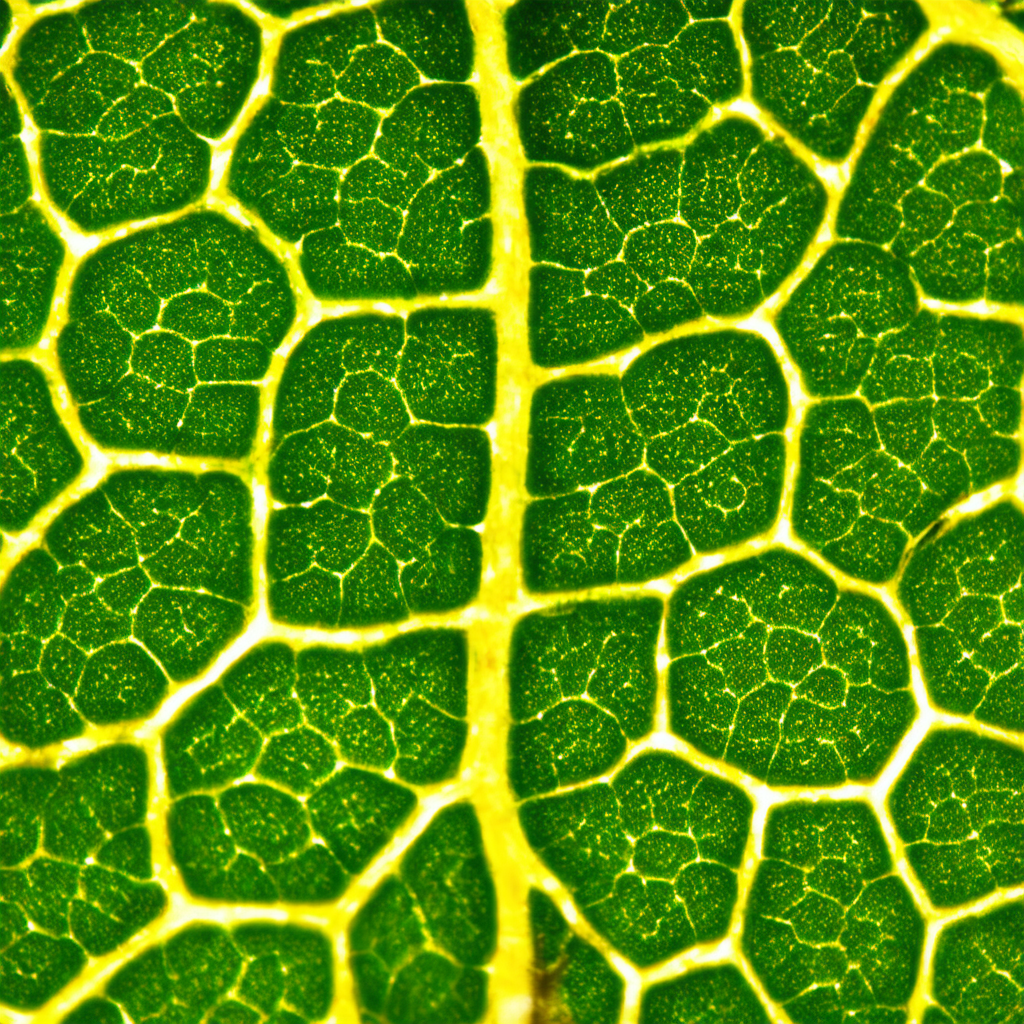
\includegraphics[width=0.19\textwidth]{../reference_images/image_grid_20240721_220650.png}\hfill
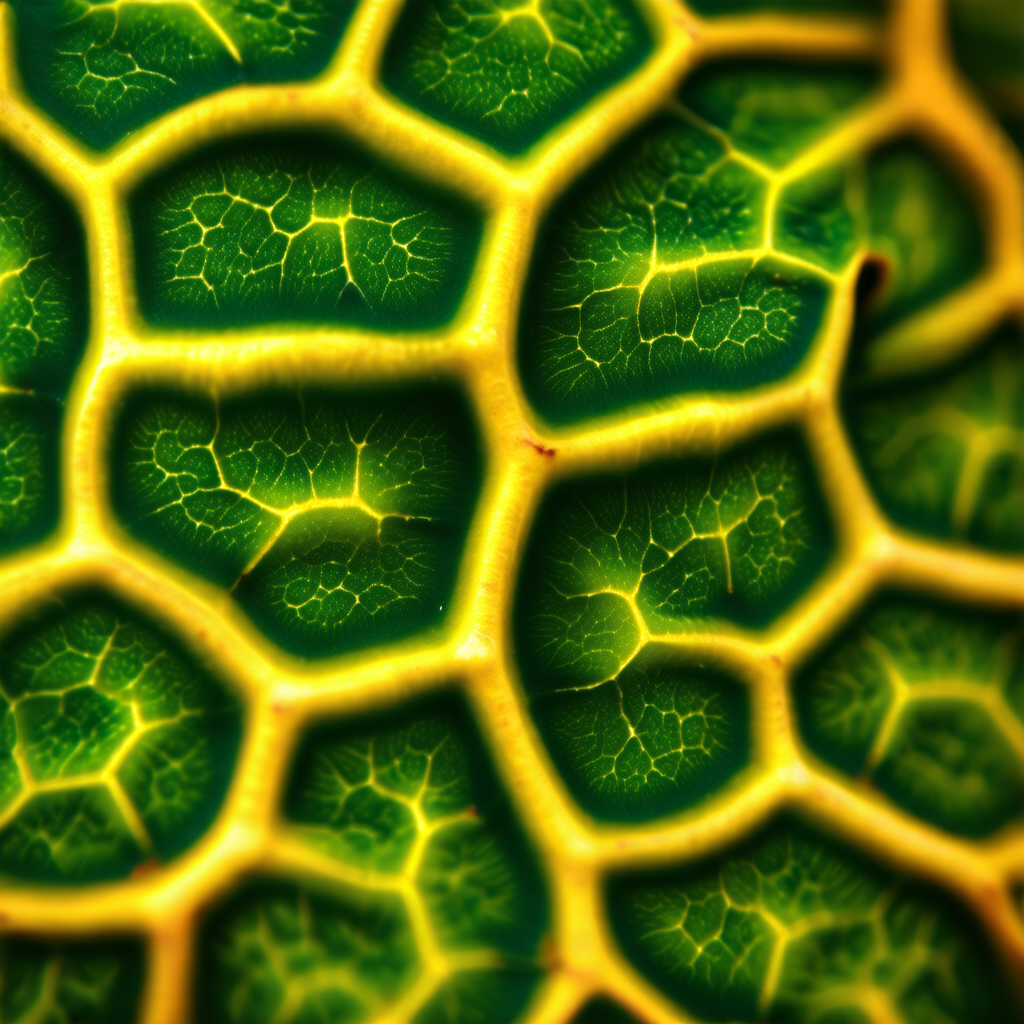
\includegraphics[width=0.19\textwidth]{../reference_images/image_grid_2-of-16__20240721_210804.png}\hfill
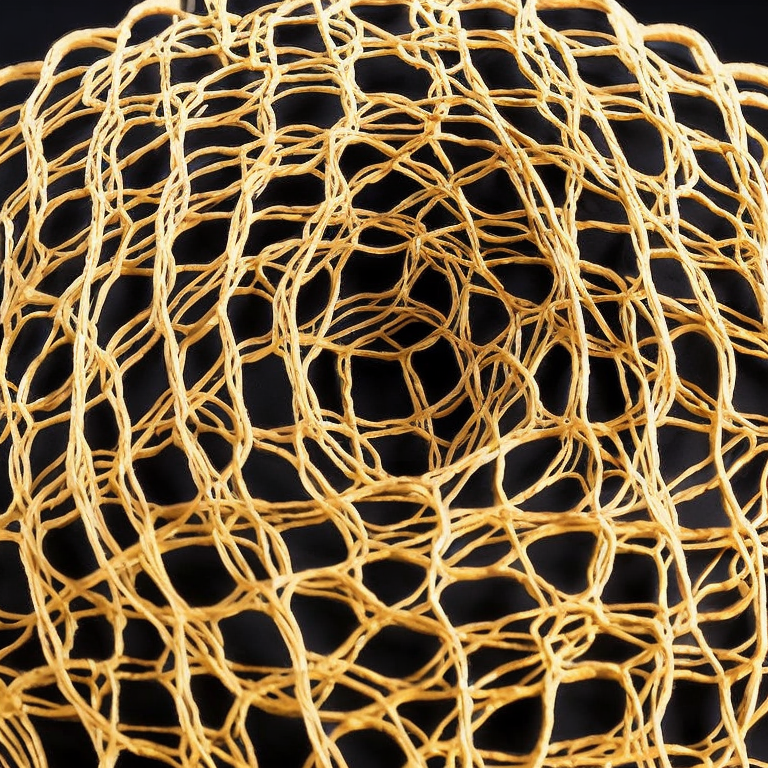
\includegraphics[width=0.19\textwidth]{../reference_images/image_grid_2-of-3__20240721_061946.png}\hfill
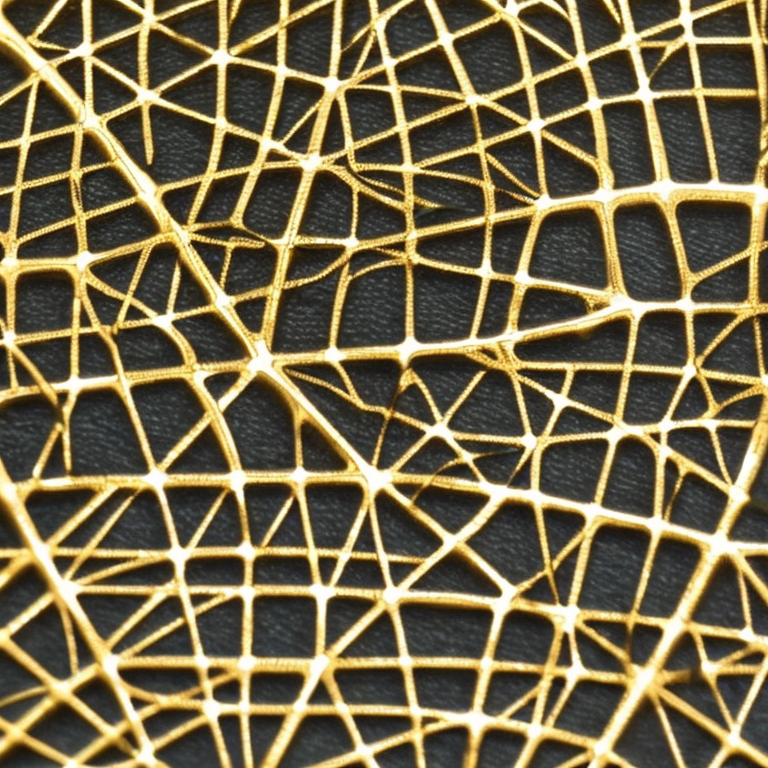
\includegraphics[width=0.19\textwidth]{../reference_images/image_grid_7-of-9__20240721_063700.png}\hfill
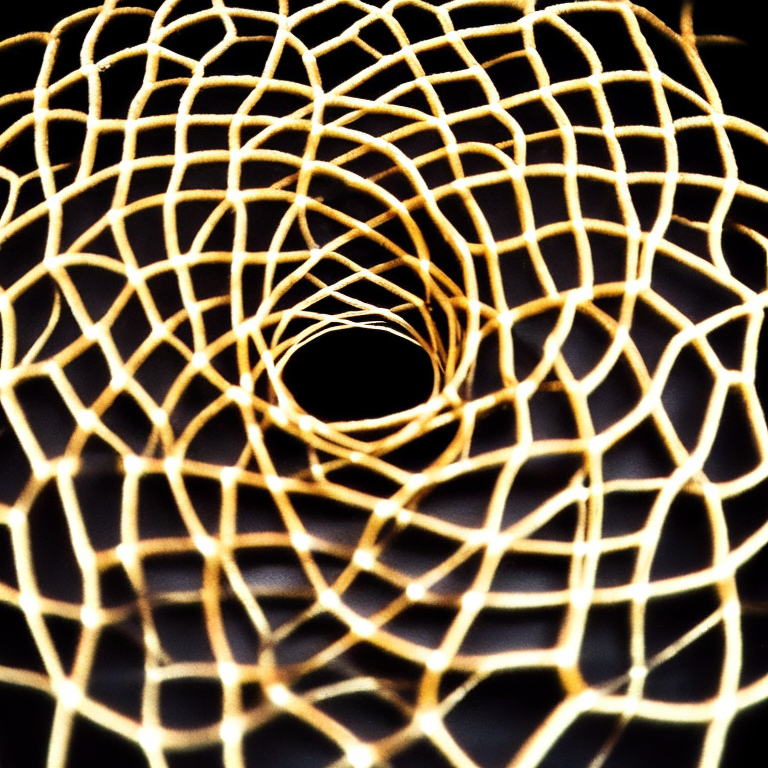
\includegraphics[width=0.19\textwidth]{../reference_images/image_grid_0-of-3__20240721_061945.png}
\caption{Reference images (left to right): hierarchical leaf venation (img1); closed-cell walls enclosing a fine open network (img2); disordered layered fibre net (img3); rectilinear crossing struts (img4); nested rings around a central void with a size gradient (img5).}
\label{fig:images}
\end{figure}

\begin{table}[H]\centering\footnotesize
\caption{Design principles extracted from the reference images, their atomistic realisation, main assumption and a plausible alternative reading.}
\label{tab:principles}
\setlength{\tabcolsep}{4pt}
\begin{tabular}{p{0.45cm}>{\raggedright\arraybackslash}p{2.1cm}>{\raggedright\arraybackslash}p{2.2cm}>{\raggedright\arraybackslash}p{4.6cm}>{\raggedright\arraybackslash}p{2.4cm}>{\raggedright\arraybackslash}p{2.4cm}}
\toprule
 & Principle & Motivating feature & Atomistic realisation & Assumption & Alternative\\
\midrule
P1 & nested hierarchy & vein widths at 3--4 scales (img1); coarse walls + fine net (img2); rings within rings (img5) & nanomesh with fine pores (period $p_1$) inside domains bounded by wider ``vein'' ligaments (width $W_2$, domain $D_2$); optional third level ($W_3$, $D_3$) & ligaments $\gtrsim 5$\,\AA{} remain stable sp$^2$ carbon; coarse scale limited by the supercell & graded ligament widths without domains; hierarchical defects\\
P2 & redundancy / loops & closed loops at every level (img1); overlaid nets (img3) & cyclomatic number of the ligament graph; closed-cell vs open patterns at equal porosity & loops counted on the relaxed bond graph & layering not accessible in one sheet\\
P3 & compart\-mentalisation & thick walls isolate cells (img2) & vein network of the two-level mesh; do cracks stop at veins? & vein width sets barrier strength & walls may act as stress concentrators\\
P4 & anisotropy & midrib direction (img1); crossing struts (img4) & slits / elliptical pores at $0/45/90^\circ$; strut families; zigzag vs armchair lattice & uniaxial loading along $x$ & lattice chirality as an atomistic anisotropy\\
P5 & scale separation & ratio $\sim$5--10 between levels (img2) & domain size $D_2$ at fixed $p_1$ (ratios 2--5) & cell must hold several domains & continuous (graded) separation\\
P6 & disorder & irregular cells (img3) & jittered / size-dispersed pore lattices; periodic Voronoi networks with tunable regularity; multiple seeds & quenched disorder & disorder of ligament width\\
P7 & tortuous paths & curved fibres (img3) & Voronoi networks, staggered lattices; descriptor tortuosity & measured on bond graph & wavy slits\\
P8 & straight through-going paths & lines spanning the field (img4) & strut lattices with/without a family along the load; slits parallel to the load & periodic continuation & staggered struts\\
P9 & node connectivity & 3--4 lines meeting at nodes (img4) & $0/60/120^\circ$ (6-connected) vs $0/90^\circ$ (4-connected) vs $30/90/150^\circ$ (no strut along load) & stretching-dominated plates & masked by node stress concentration\\
P10 & gradients & shrinking cells (img5) & pore-size gradient along $x$ or radial & gradient wavelength limited by cell & ligament-width gradient\\
P11 & nesting around a flaw & rings around a hole (img5) & hole + concentric rings of small pores vs bare hole vs hole + uniform far-field pores at matched porosity & halo changes the hole stress field & rings add crack nuclei\\
\bottomrule
\end{tabular}
\end{table}

\section{Generated carbon architecture space}
\label{sec:space}
All candidates are explicit carbon atoms in orthorhombic periodic supercells ($x$ and $y$ periodic, vacuum along $z$), represented as ASE \texttt{Atoms} objects~\cite{ase} that carry generator family, parameters and random seed in their metadata. Structures are derived from a rectangular graphene sheet at the \rebo{} equilibrium lattice constant ($a_0 = 2.4602$\,\AA) by atom removal (pores, slits, cracks, vacancies), followed by iterative pruning of atoms with fewer than two neighbours, removal of disconnected fragments, and relaxation. Ten generator families instantiate the principles of Table~\ref{tab:principles}: \texttt{pristine}, \texttt{nanomesh\_single}, \texttt{nanomesh\_hier} (two- and three-level nested meshes), \texttt{voronoi\_network}, \texttt{slit\_array}, \texttt{strut\_lattice}, \texttt{graded\_pores}, \texttt{ring\_around\_hole}, \texttt{precrack} and \texttt{vacancies}. For every controlled comparison the free size parameter of each family is adjusted by bisection so that the porosity of the generated structure matches a target ($\phi = 0.20\pm0.01$ unless stated), which fixes carbon mass and footprint across architectures. Descriptors are measured on the relaxed structures (not taken from generator parameters): porosity, areal density, coordination statistics, fraction of two-coordinated edge atoms, bond-graph cyclomatic number per atom (redundancy), load-path tortuosity (shortest periodic bond path across $x$ divided by $L_x$), pore-size and ligament-width distributions from Euclidean distance transforms of a periodic raster, the minimum load-bearing solid fraction across the loading direction (bottleneck), a structure-tensor anisotropy index, and hierarchy metrics (number of distinct pore/ligament scales, scale ratio, coarse-ligament solid fraction).

\subsection{Hierarchy as a controlled multivariable design axis}
The hierarchy ladder (Fig.~\ref{fig:space}) spans, at matched porosity and footprint (120\,\AA{} cells): single-scale meshes with fine (12\,\AA), reference (16\,\AA) and coarse (32\,\AA) periods, the coarse level alone (square pores on the 40\,\AA{} vein grid), two-level nested meshes with domain sizes 24/40/60\,\AA{} (scale ratios 2, 3.3, 5 relative to the 12\,\AA{} fine period) and vein widths 4/8/12\,\AA, and a three-level mesh (10\,\AA{} period, 30\,\AA{} domains with 5\,\AA{} veins, 120\,\AA{} domains with 12\,\AA{} veins). Hierarchy depth, scale ratio, inter-level ligament width, inter-level connectivity (fine ligaments attach to veins), and the organisation of hierarchy relative to the load are therefore separately variable.

\section{Force field}
\label{sec:ff}
The authoritative production potential is the screened second-generation REBO potential for carbon (\rebo{}, ``Rebo2Scr'')~\cite{brenner2002,pastewka2008,pastewka2013} in the parameterisation and implementation of Atomistica 1.2.7~\cite{atomistica} (default parameters: $C_\mathrm{min}=1$, $C_\mathrm{max}=2$, dihedral term off, default $P_{CC}$, $F_{CC}$ tables). The energy is
\begin{equation}
E=\sum_{i<j} f^{ar}_{ij}\left[V_R(r_{ij})+\bar b_{ij}V_A(r_{ij})\right],\qquad
\bar b_{ij}=\tfrac12\left(b_{ij}+b_{ji}+F_{CC}(N^t_i,N^t_j,N^{conj}_{ij})\right),
\end{equation}
\begin{equation}
b_{ij}=\Big(1+\sum_{k\neq i,j} f^{bo}_{ik}\,g(\cos\theta_{jik},N^t_i)+P_{CC}(N^H_i,N^C_i)\Big)^{-1/2},
\end{equation}
with the screened cut-off functions $f^{x}_{ij}=(1-f^{in}_{ij})S_{ij}f^{x}(r_{ij})+f^{in}_{ij}$ ($x\in\{ar,bo,nc\}$) and the elliptical screening function $S_{ij}=\prod_k S(C_{ijk})$, $S(C)=\exp[-((C_\mathrm{max}-C)/(C-C_\mathrm{min}))^2]$ for $C_\mathrm{min}<C<C_\mathrm{max}$ (0 below, 1 above), $C_{ijk}=[2(x_{ik}+x_{jk})-(x_{ik}-x_{jk})^2-1]/[1-(x_{ik}-x_{jk})^2]$, $x_{ik}=r_{ik}^2/r_{ij}^2$. Cut-off radii are 1.95--2.25\,\AA{} (inner), 2.179--2.820\,\AA{} (pair), 1.866--2.758\,\AA{} (bond order) and 1.217--4.000\,\AA{} (neighbour count / conjugation). No parameter, screening function or cut-off was modified. Every run record stores the potential name, implementation, version, literature references, source commit, a SHA-256 checksum of the published parameters and tables, and the units.

\section{Implementation}
\label{sec:impl}
\textbf{TorchRebo2Scr.} A GPU-native PyTorch~\cite{pytorch} implementation was written by transcribing the Atomistica kernel (\texttt{bop\_kernel\_rebo2.f90} with the \texttt{SCREENING}, \texttt{NUM\_NEIGHBORS} and trigonometric cut-off options, \texttt{rebo2\_func.f90}, \texttt{rebo2\_db.f90}, \texttt{rebo2\_default\_tables.f90}, \texttt{table2d.f90}, \texttt{table3d.f90}). The angular spline coefficients and the bicubic/tricubic table coefficients are obtained by solving the same linear systems as the Fortran code; the single-precision Fortran literals of the angular knot values are reproduced deliberately (without this detail the two implementations differ by $10^{-8}$\,eV/atom). Energies are evaluated with dense, padded neighbour tensors ($[N,M]$ pairs within 4.0\,\AA{}+skin for screening and coordination, $[N,M_b]$ pairs within 2.82\,\AA{}+skin for pair energies and bond order, $[N,M,M]$ screening triplets, $[N,M_b,M_b]$ angular triplets); forces are exact gradients by automatic differentiation, $\mathbf F=-\partial E/\partial\mathbf R$, and the virial is $\partial E/\partial\boldsymbol\varepsilon$ for an affine strain of all pair vectors. Per-atom energies (half of each pair energy) and per-atom virials (pair-vector decomposition) are available for visualisation. Value caps of the neighbour counts ($N\le4$, $N^t\le3$, $N^{conj}\le8$) are implemented with straight-through gradients so that forces coincide with Atomistica's even in over-coordinated environments. Degenerate screening geometries ($k$ projecting exactly onto $i$ or $j$, contribution exactly 1) are excluded from the product to keep the float32 backward pass free of $0/0$. The engine runs on \texttt{mps} (Apple GPU, float32), \texttt{cuda} (float32/64) and \texttt{cpu} (float32/64) with automatic backend detection; the campaign used MPS float32 (``fast discovery mode''); CPU float64 is the ``reference mode''.

\textbf{Neighbour lists.} Pair lists are built with a cell-list algorithm (ASE \texttt{primitive\_neighbor\_list}, $O(N)$), padded to dense tensors, sorted by distance so that the short list is a prefix of the long list, and equipped with reverse-pair indices for periodic images. A Verlet skin of 0.3\,\AA{} with a half-skin displacement criterion (checked every FIRE iteration relative to the affine image of the build-time positions) triggers rebuilds. The optimised list is validated against brute-force enumeration (TEST~9).

\textbf{Batching.} Several independent structures are concatenated into one ``super-system'' (per-atom structure index, per-structure cells and strain tensors); energies, forces, virials, FIRE state and convergence are handled per structure, so a whole batch is relaxed in one sequence of device kernels. Because the MPS backend is limited by per-kernel launch overhead rather than by arithmetic, several independent processes scale linearly on one GPU; the campaign was executed by a job queue with 3--5 concurrent workers.

\textbf{Minimisation and AQS.} A batched FIRE minimiser~\cite{bitzek2006} (ASE parameters: $\Delta t=0.1$, $\Delta t_\mathrm{max}=1$, $\alpha=0.1$, per-atom step limit 0.2\,\AA) relaxes all atoms to $|F|_\mathrm{max}<0.02$\,eV/\AA{} (0.005 in reference runs). The AQS protocol applies uniaxial engineering strain along $x$ in increments of 0.5\% (affine mapping of positions and cell), predicts the transverse strain from the previous Poisson slope, relaxes the atoms, then relaxes the transverse cell dimension to $\sigma_{yy}=0$ by secant iterations with a trust region of 0.5\% (uniaxial-stress state), and records the 2D stress $\sigma=(1/A)\,\partial E/\partial\boldsymbol\varepsilon$ in N/m ($1$\,eV/\AA$^2$ = 16.02\,N/m), per-atom energies and virials, the bond topology and every bond-breaking event with its location. The first bond-breaking event is bracketed by bisection of the increment down to 0.125\%. A structure stops when its bond network no longer percolates across the loading direction, when the stress falls below 10\% (5\% in Stage~1) of its peak after damage, 12\% strain beyond the peak (Stage~2 onward; 35\% total in Stage~1), or at 32\% strain. Before loading, the cell is relaxed to zero in-plane stress; all strains refer to that reference cell. Bond connectivity for analysis uses $r<2.0$\,\AA{} (documented in Sec.~\ref{sec:damage}).

\section{Validation}
\label{sec:validation}
Validation preceded the discovery study (Table~\ref{tab:validation}; Figs.~\ref{fig:agreement}--\ref{fig:refaqs}). The Torch implementation reproduces Atomistica energies, forces and stresses to double-precision round-off ($\le 10^{-13}$\,eV/atom, $\le 10^{-12}$\,eV/\AA) for pristine, displaced, strained, defected, pore-edge, crack-tip and near-/post-rupture configurations; finite-difference forces and stresses, neighbour-list, translation-, force-balance- and periodic-image invariances pass; the relaxed lattice constant (2.460177\,\AA), bond length (1.420384\,\AA), cohesive energy ($-7.395110$\,eV/atom), elastic constants ($C_{11}=289.5$, $C_{12}=113.5$, $Y_{2D}=245.1$\,N/m, $\nu=0.392$) and the homogeneous tensile responses (zigzag peak 37.7\,N/m, armchair 30.5\,N/m) coincide with Atomistica. The fast float32 MPS mode deviates from the reference by $\sim10^{-6}$\,eV/atom, $\sim10^{-4}$\,eV/\AA{} and $\sim10^{-5}$\,N/m, including at pre-damage, peak and post-peak frames, i.e. two orders of magnitude below the minimisation tolerance; repeated evaluations on MPS differ by reduction-order round-off only ($10^{-7}$ relative). The elastic constants expose the known deficiency of REBO2 (experiment: $Y_{2D}\approx340$\,N/m, $\nu\approx0.17$~\cite{lee2008}), which we report rather than correct.

\subsection{Bond-separation validation}
\label{sec:bondsep}
Fig.~\ref{fig:bondsep} shows $E(r)$ and $F(r)=-\mathrm dE/\mathrm dr$ through complete rupture for an isolated C$_2$ dimer, a bond inside a periodic graphene sheet (one atom pulled along the bond), a crack-tip atom pulled open, and the homogeneous affine stretch of zigzag and armchair sheets to 80\% strain. The Torch curves reproduce Atomistica to $10^{-11}$\,eV/\AA{} (cpu float64) and to $\sim10^{-2}$\,eV/\AA{} on forces up to $10^3$\,eV/\AA{} (float32). Three features of the published potential are documented: (i) the isolated dimer shows the familiar cut-off ``bump'' in the force tail (2.2--2.8\,\AA) because no neighbour screens the pair; (ii) when a pulled atom crosses the screening ellipse of a neighbouring pair, the screening function switches on/off over a narrow range and produces steep but continuous force features; (iii) the affinely stretched lattice re-stiffens for $\varepsilon>0.6$ (bonds beyond 2.2\,\AA), a regime never reached by relaxed AQS trajectories because the lattice loses stability near 25\% strain. No spurious discontinuities beyond those intrinsic to the published functional form were found, so the discovery campaign proceeded.

\subsection{Convergence and protocol checks}
Convergence with respect to the FIRE tolerance, the strain increment (with and without bisection refinement) and the system size (periodic repeats of a mesh pattern; a fixed crack in growing cells) is summarised in Table~\ref{tab:validation} (TESTS~13--15) and Fig.~\ref{fig:convergence}; TEST~18 compares complete stress--strain curves of the Torch-driven AQS with an AQS driven by the Atomistica backend and ASE's FIRE under the same protocol (Fig.~\ref{fig:refaqs}). A protocol finding worth recording: under zigzag tension the homogeneous \rebo{} lattice exhibits a bistable transverse response above $\approx16\%$ strain (two branches of $\sigma_{yy}(\varepsilon_y)$ at fixed $\varepsilon_x$), so transverse relaxation must follow the current branch continuously; the trust region of the secant scheme was chosen accordingly. All porous structures fail well below this strain.

\section{Numerical precision and computational performance}
\label{sec:perf}
Fig.~\ref{fig:precision} quantifies the fast-versus-reference differences per configuration; Fig.~\ref{fig:performance} reports throughput. Interpretation and numbers are given in the figure captions and in Table~\ref{tab:validation}.

The port is exact but not faster than the reference per evaluation. On the delivery machine (Apple M4 Max, no CUDA device) the GPU evaluation of energy, forces and virial (MPS, float32) costs about 9\,$\mu$s per atom for systems above 3000 atoms and is launch-bound below that size, whereas the single-threaded Fortran reference costs about 3\,$\mu$s per atom (Fig.~\ref{fig:performance}). The campaign nevertheless ran on the Torch engine because it provides what the reference does not: batched evaluation of several structures in one call, per-atom energies and virials for the damage analysis, analytic forces and stresses obtained by automatic differentiation of the same energy code, and concurrent use of the GPU by several simulation processes (1.7--2.1 times the single-process throughput with 2--4 processes, the mode used by the job queue). No result depends on the choice of engine: every quantity that can be checked against the reference was checked (TESTS~1--4, 16--19), including complete stress--strain curves through fracture (TEST~18). The CUDA code path is identical but was not benchmarked.

\section{Experimental strategy}
\label{sec:strategy}
The discovery study proceeded in stages, each recorded in the experiment database with the reason for every simulation: (1) baselines; (2) broad reconnaissance of the image-derived design variables at matched porosity; (3) formation of competing mechanistic hypotheses from the observations; (4) discriminating simulations with matched pairs and recorded predictions; (5) deep mechanism studies (scaling, thresholds, interactions); (6) random-seed replication of stochastic structures; (7) recorded predictions for unseen designs; (8) holdout evaluation. Selection of later experiments used the earlier results (hypothesis discrimination, regime boundaries, outliers, Pareto refinement); no machine-learning surrogate replaced the simulator.

\section{Force-field validation figures}
\begin{figure}[H]\centering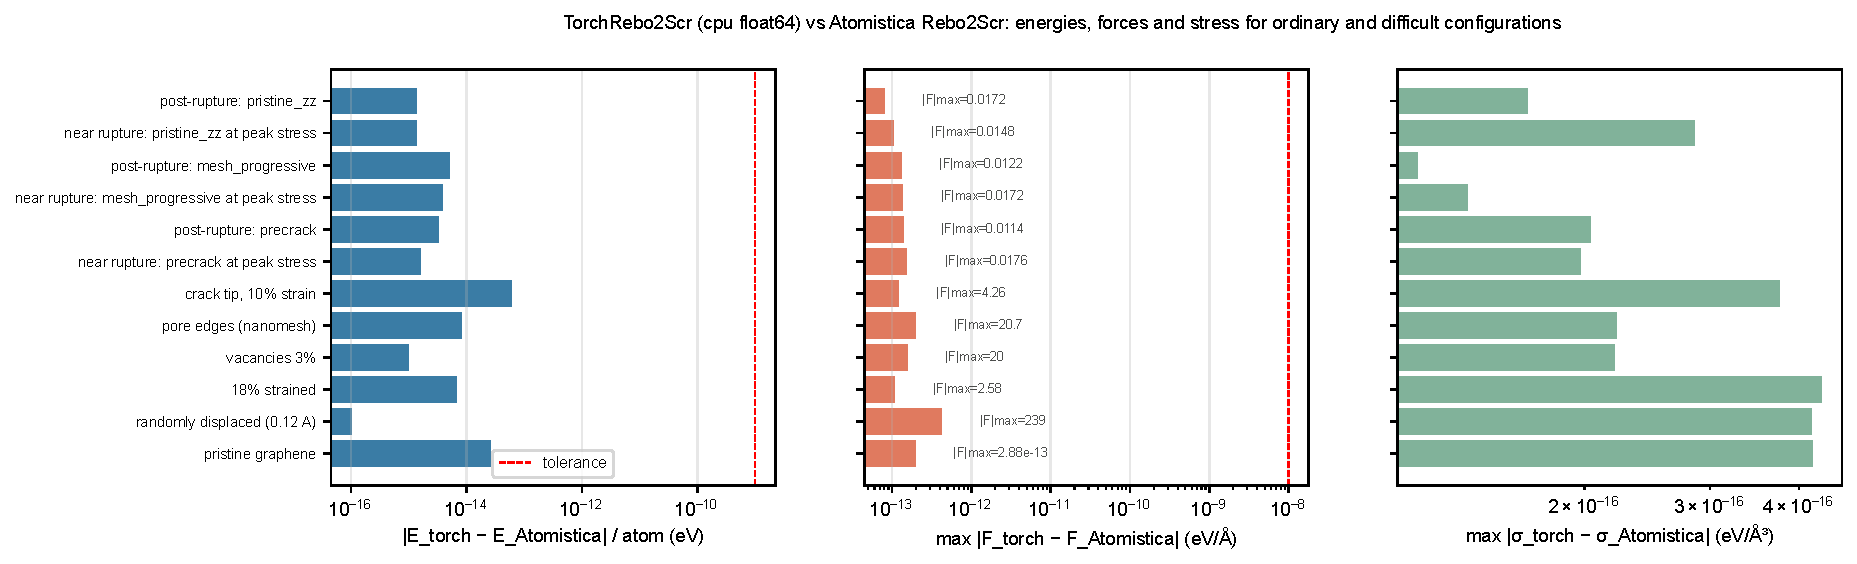
\includegraphics[width=1.0\textwidth]{validation/agreement_with_reference.pdf}\caption{Agreement between the PyTorch implementation of screened REBO2 (cpu, float64) and the authoritative Atomistica Rebo2Scr implementation for 12 configuration classes including pore edges, crack tips and near-rupture/post-rupture frames taken from AQS trajectories. Bars: per-atom energy difference, maximum force-component difference (annotated with the largest force magnitude of the configuration) and maximum stress-component difference. Dashed lines: acceptance tolerances (1e-9 eV/atom, 1e-8 eV/A). All differences are at the level of double-precision round-off.}\label{fig:agreement}\end{figure}
\begin{figure}[H]\centering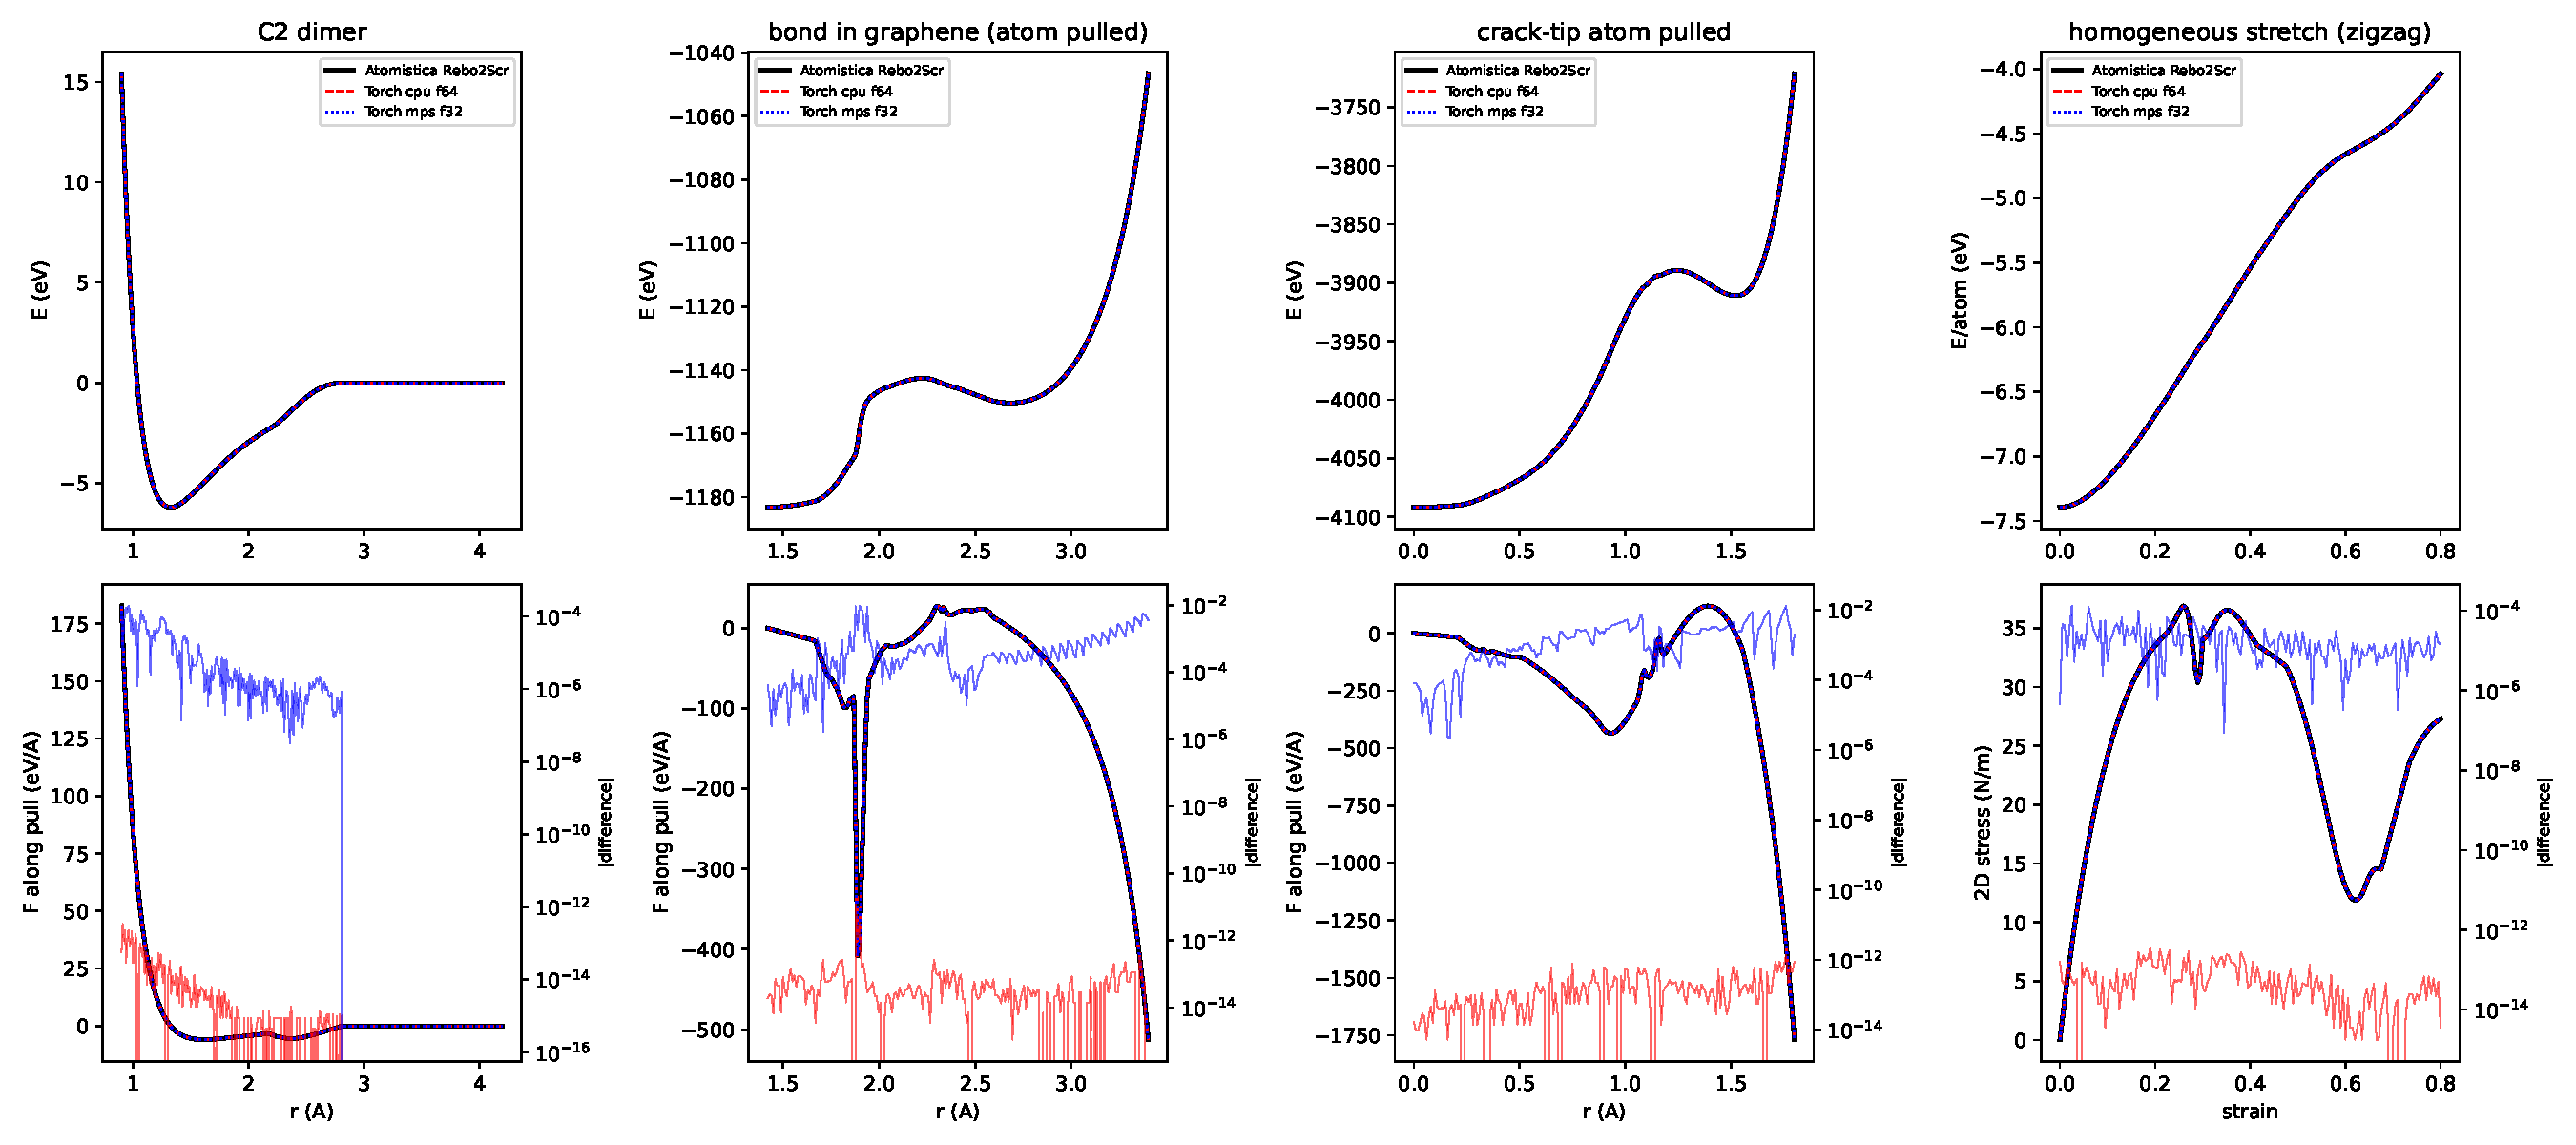
\includegraphics[width=1.0\textwidth]{validation/bond_separation.pdf}\caption{Bond-separation validation (TEST 19). Top: energy, bottom: force along the pulling direction (or 2D stress for the homogeneous stretch) for the C$\_2$ dimer, a bond in graphene (one atom pulled along the bond), a crack-tip atom pulled open, and the affine stretch of a zigzag sheet; black: Atomistica Rebo2Scr, red dashed: Torch cpu float64, blue dotted: Torch MPS float32; thin lines (right axes): absolute differences. Sharp features are intrinsic to the published screening/cut-off functions and are reproduced identically.}\label{fig:bondsep}\end{figure}
\begin{figure}[H]\centering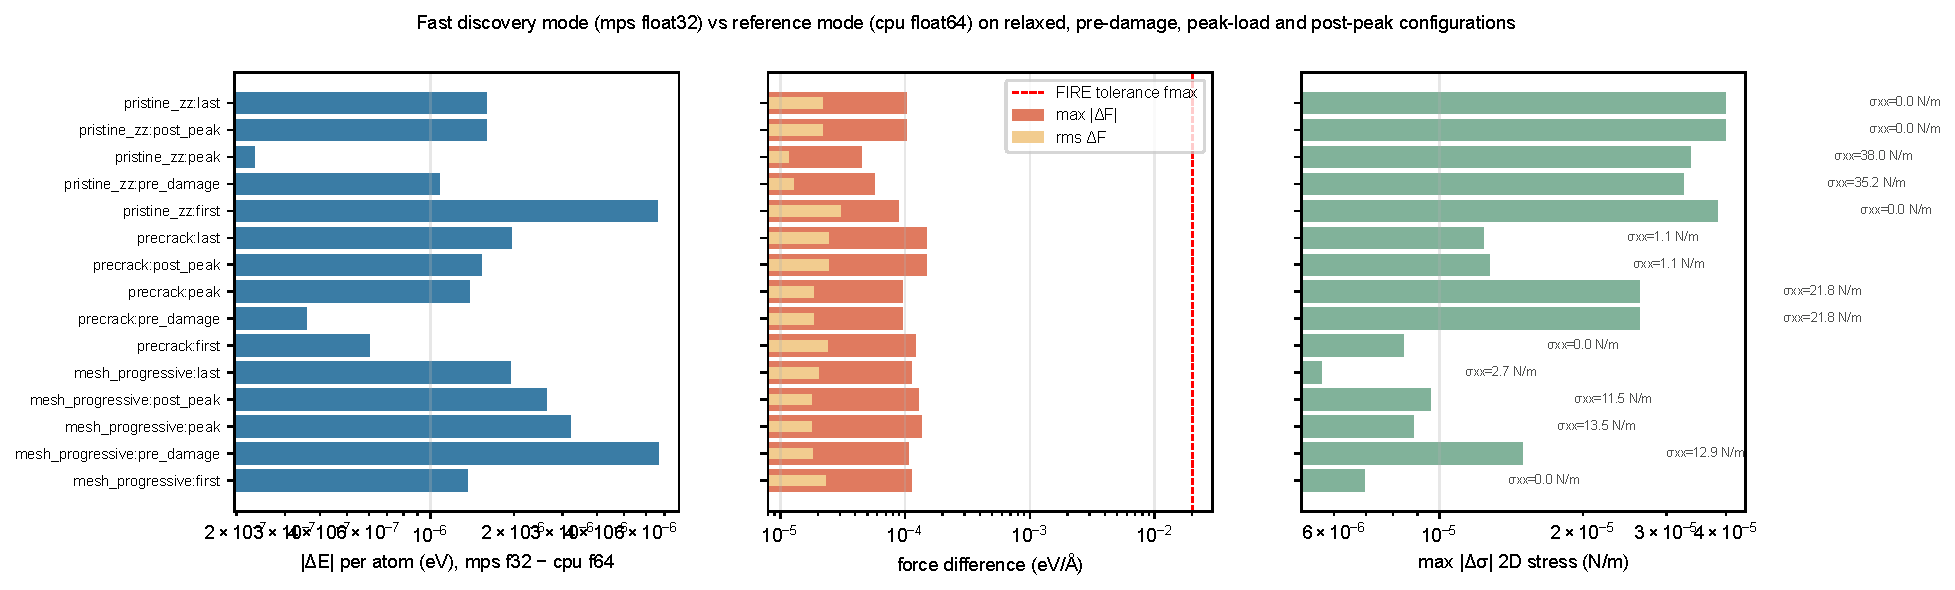
\includegraphics[width=1.0\textwidth]{validation/precision_fast_vs_reference.pdf}\caption{Numerical precision of the fast discovery mode (Apple MPS, float32) relative to the reference mode (cpu, float64, identical to Atomistica) for frames taken from three AQS trajectories (progressive nanomesh, precracked sheet, pristine zigzag graphene): relaxed, pre-damage, peak-load, post-peak and final frames. Energy differences are ~1e-6 eV/atom, force differences ~1e-4 eV/A (two orders of magnitude below the minimisation tolerance of 0.02 eV/A), 2D-stress differences ~1e-5 N/m.}\label{fig:precision}\end{figure}
\begin{figure}[H]\centering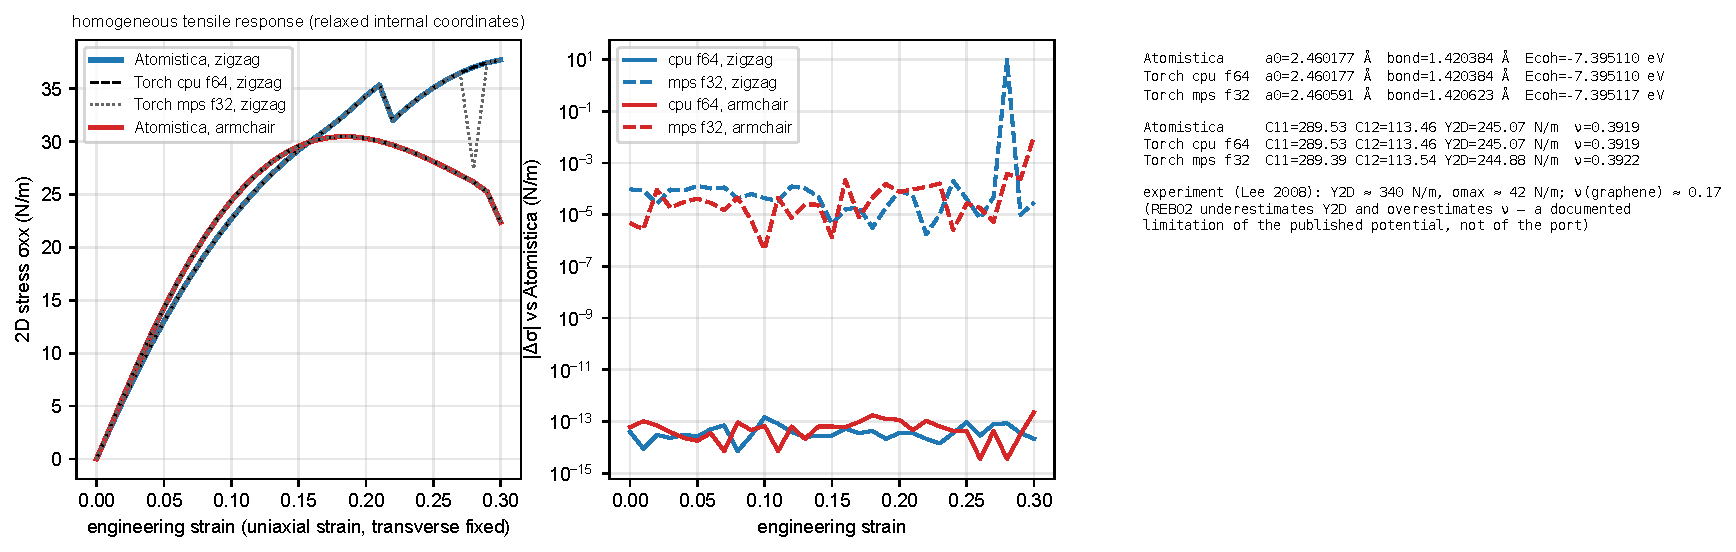
\includegraphics[width=1.0\textwidth]{validation/material_properties.pdf}\caption{Lattice constant, bond length, cohesive energy, elastic constants and homogeneous tensile response (zigzag and armchair loading, fixed transverse strain, relaxed internal coordinates) of graphene from the Torch implementation compared with Atomistica. Left: stress-strain curves; middle: absolute stress differences; right: tabulated properties with experimental reference values.}\label{fig:material}\end{figure}
\begin{figure}[H]\centering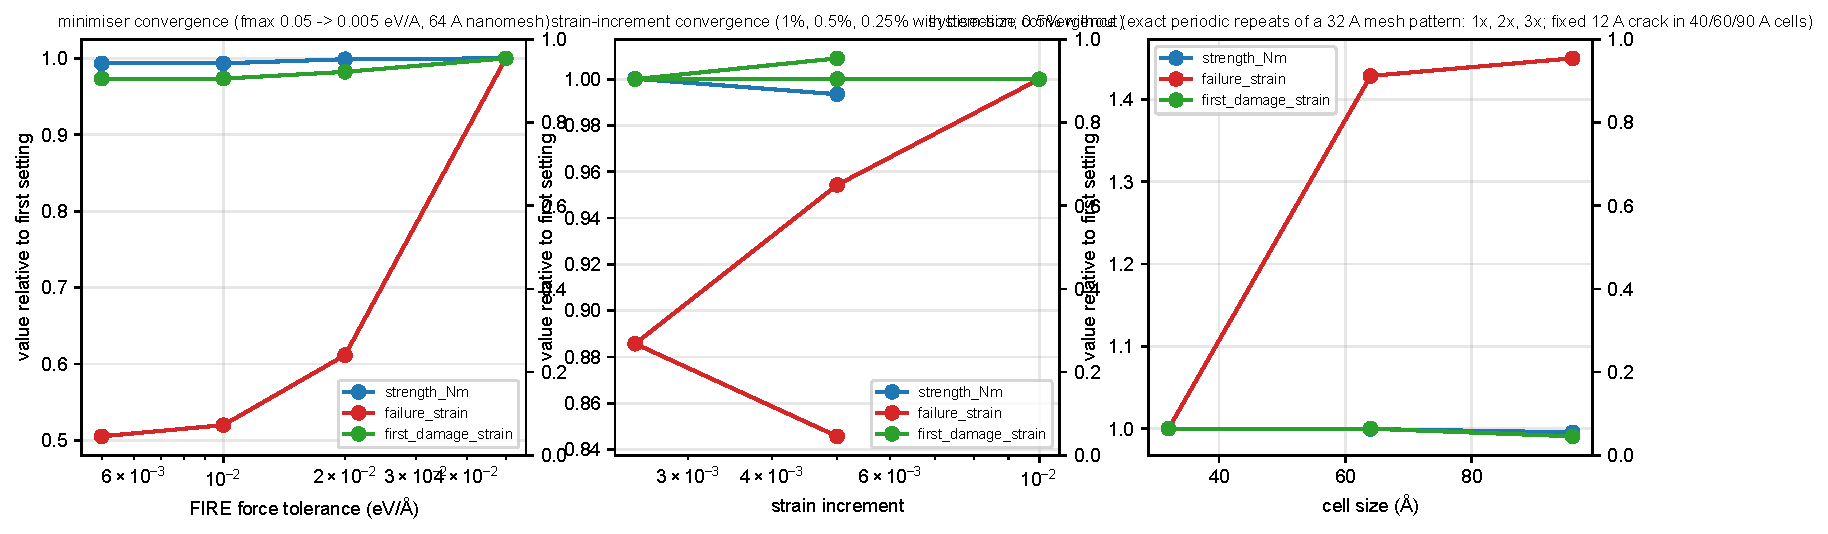
\includegraphics[width=1.0\textwidth]{validation/convergence.pdf}\caption{Convergence tests: strength, failure strain and first-damage strain of a 64 A nanomesh as a function of the FIRE force tolerance (TEST 13) and of the strain increment with/without bisection refinement (TEST 14), and size dependence for periodic repeats of the same mesh pattern and for a fixed crack in cells of increasing size (TEST 15); values normalised by the first setting.}\label{fig:convergence}\end{figure}
\begin{figure}[H]\centering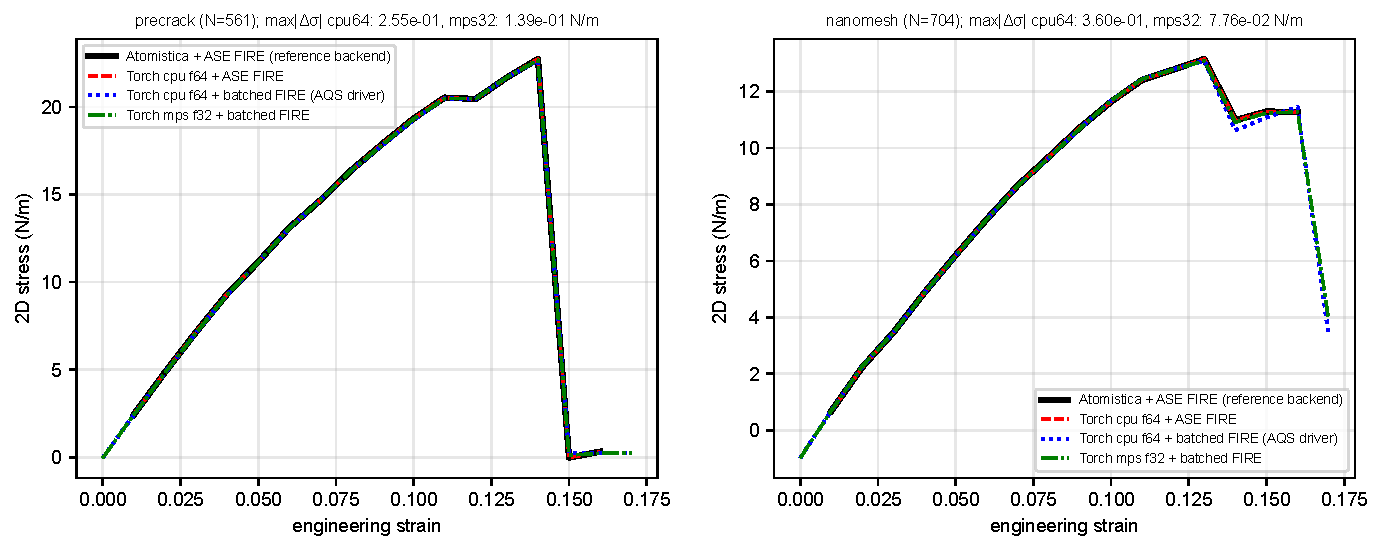
\includegraphics[width=1.0\textwidth]{validation/reference_backend_aqs.pdf}\caption{TEST 18: complete AQS stress-strain curves (uniaxial strain, fixed transverse, 1\% increments, FIRE fmax = 0.02 eV/A) for a precracked sheet and a nanomesh obtained with the authoritative backend (Atomistica + ASE FIRE) and with the Torch engine in three configurations (ASE FIRE / batched FIRE driver, cpu float64 and mps float32).}\label{fig:refaqs}\end{figure}
\begin{figure}[H]\centering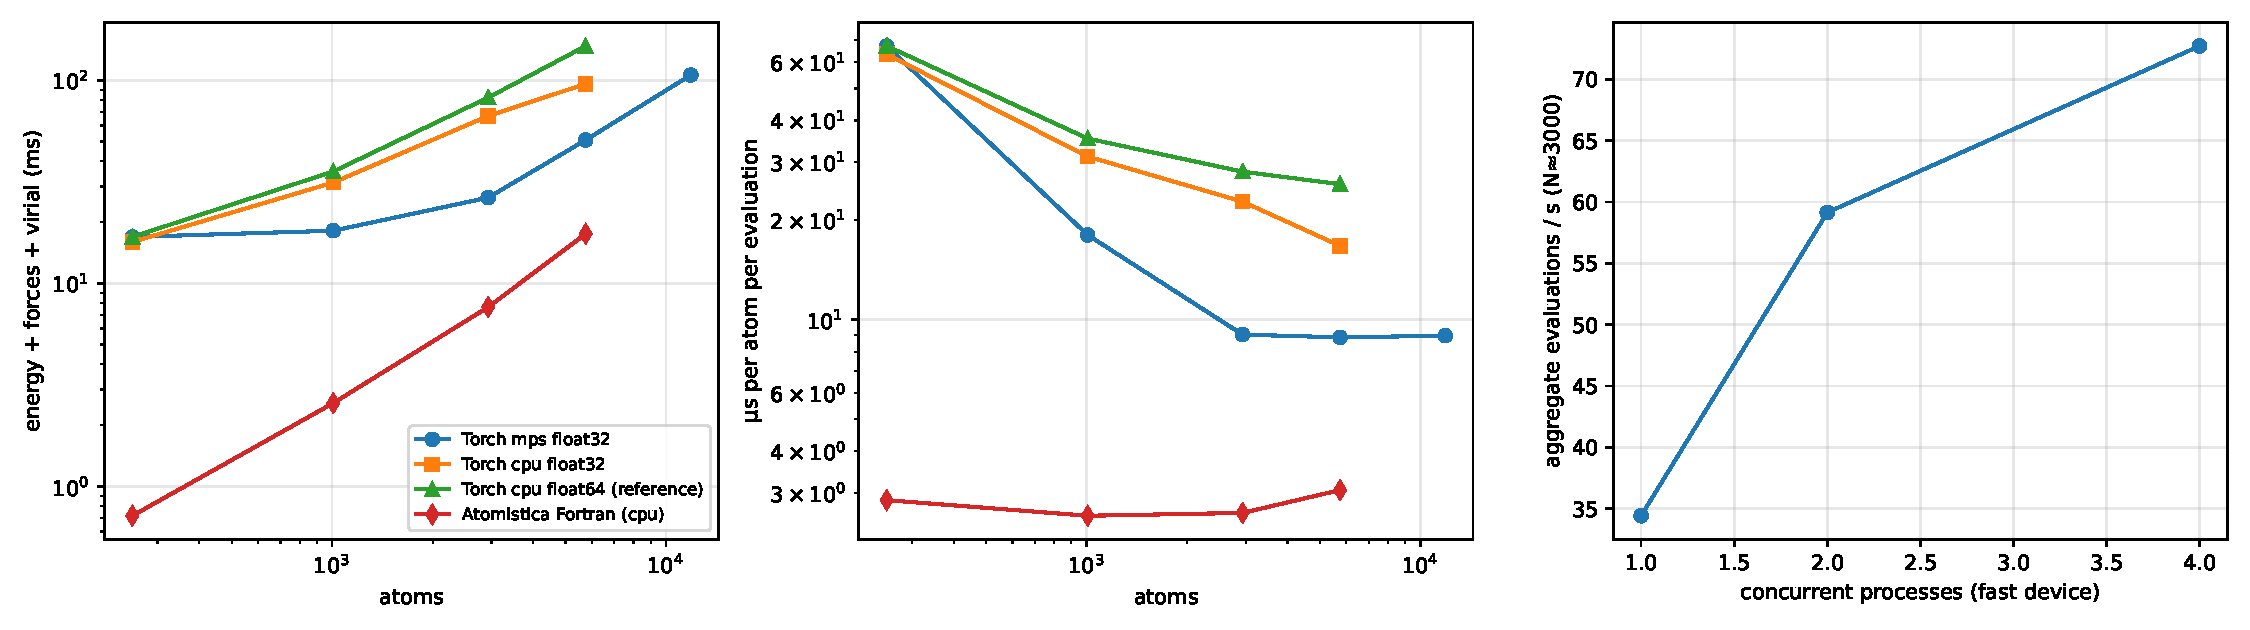
\includegraphics[width=1.0\textwidth]{validation/performance.pdf}\caption{Performance of the force engines on the delivery machine (Apple M4 Max, 16 CPU cores, 128 GB; torch 2.7.0). Left: wall time per evaluation of energy, forces and virial (mean of repeated evaluations after warm-up) for the PyTorch port on the Metal GPU (mps, float32), on the CPU (float32 and float64 reference) and for the Atomistica Fortran reference (CPU, float64, energy, forces and virial); centre: the same data per atom. The GPU port becomes launch-bound below about 3000 atoms and reaches about 9 microseconds per atom per evaluation for larger systems, which is about three times slower than the single-threaded Fortran reference per evaluation on this machine; the Fortran code does not provide per-atom virials or batched evaluation of many structures and the GPU port does not benefit from kernel fusion on MPS. Right: aggregate throughput (evaluations per second, about 3000 atoms) when several independent simulation processes share the GPU, the mode used by the campaign job queue; two to four concurrent processes give 1.7 to 2.1 times the single-process throughput. Numbers are in validation/results/performance.json.}\label{fig:performance}\end{figure}
\begin{figure}[H]\centering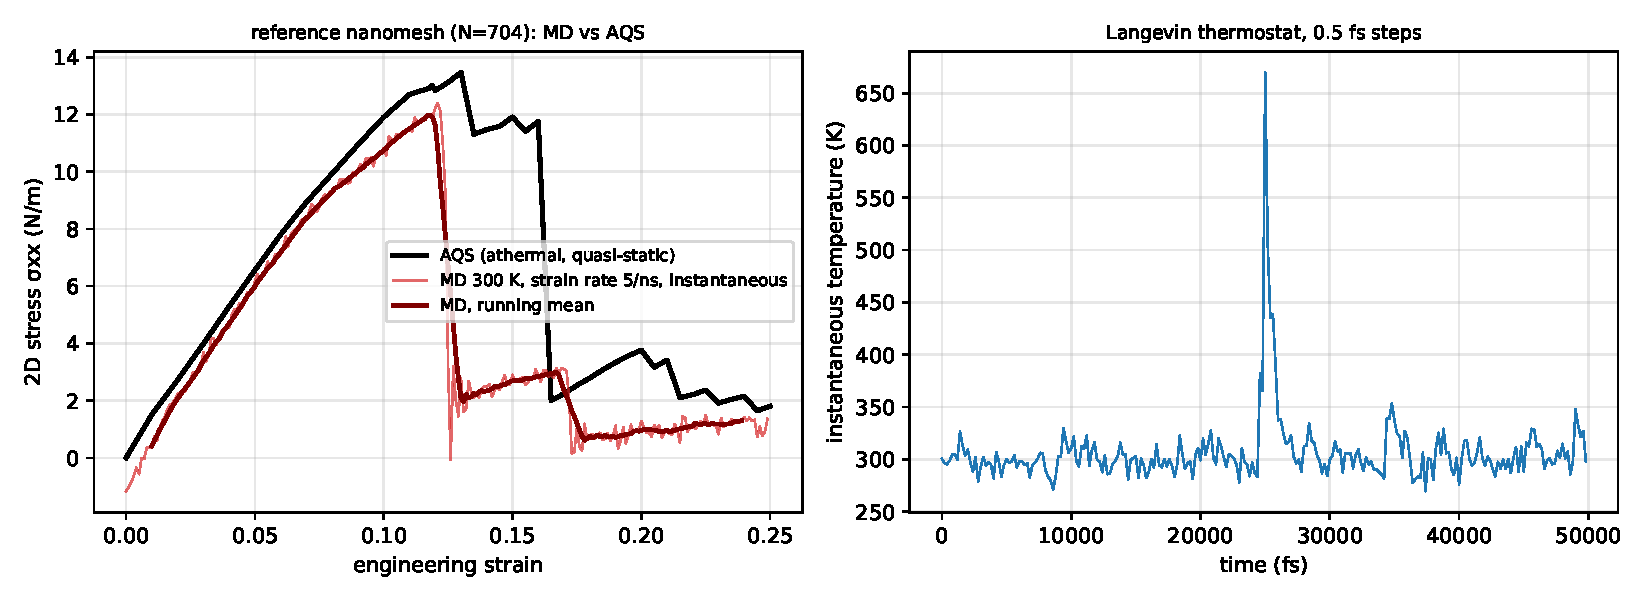
\includegraphics[width=0.9\textwidth]{validation/md_vs_aqs.pdf}\caption{Optional finite-temperature check: constant-strain-rate MD (Langevin, 300 K, 5/ns, fixed transverse strain) of the reference nanomesh compared with the AQS curve of the same structure (uniaxial stress). Peak stress MD (running mean) 12.0 N/m vs AQS 13.5 N/m; thermal activation and the biaxial stress state of the fixed-transverse MD both lower the peak.}\label{fig:md}\end{figure}
\section{Design space}
\begin{figure}[H]\centering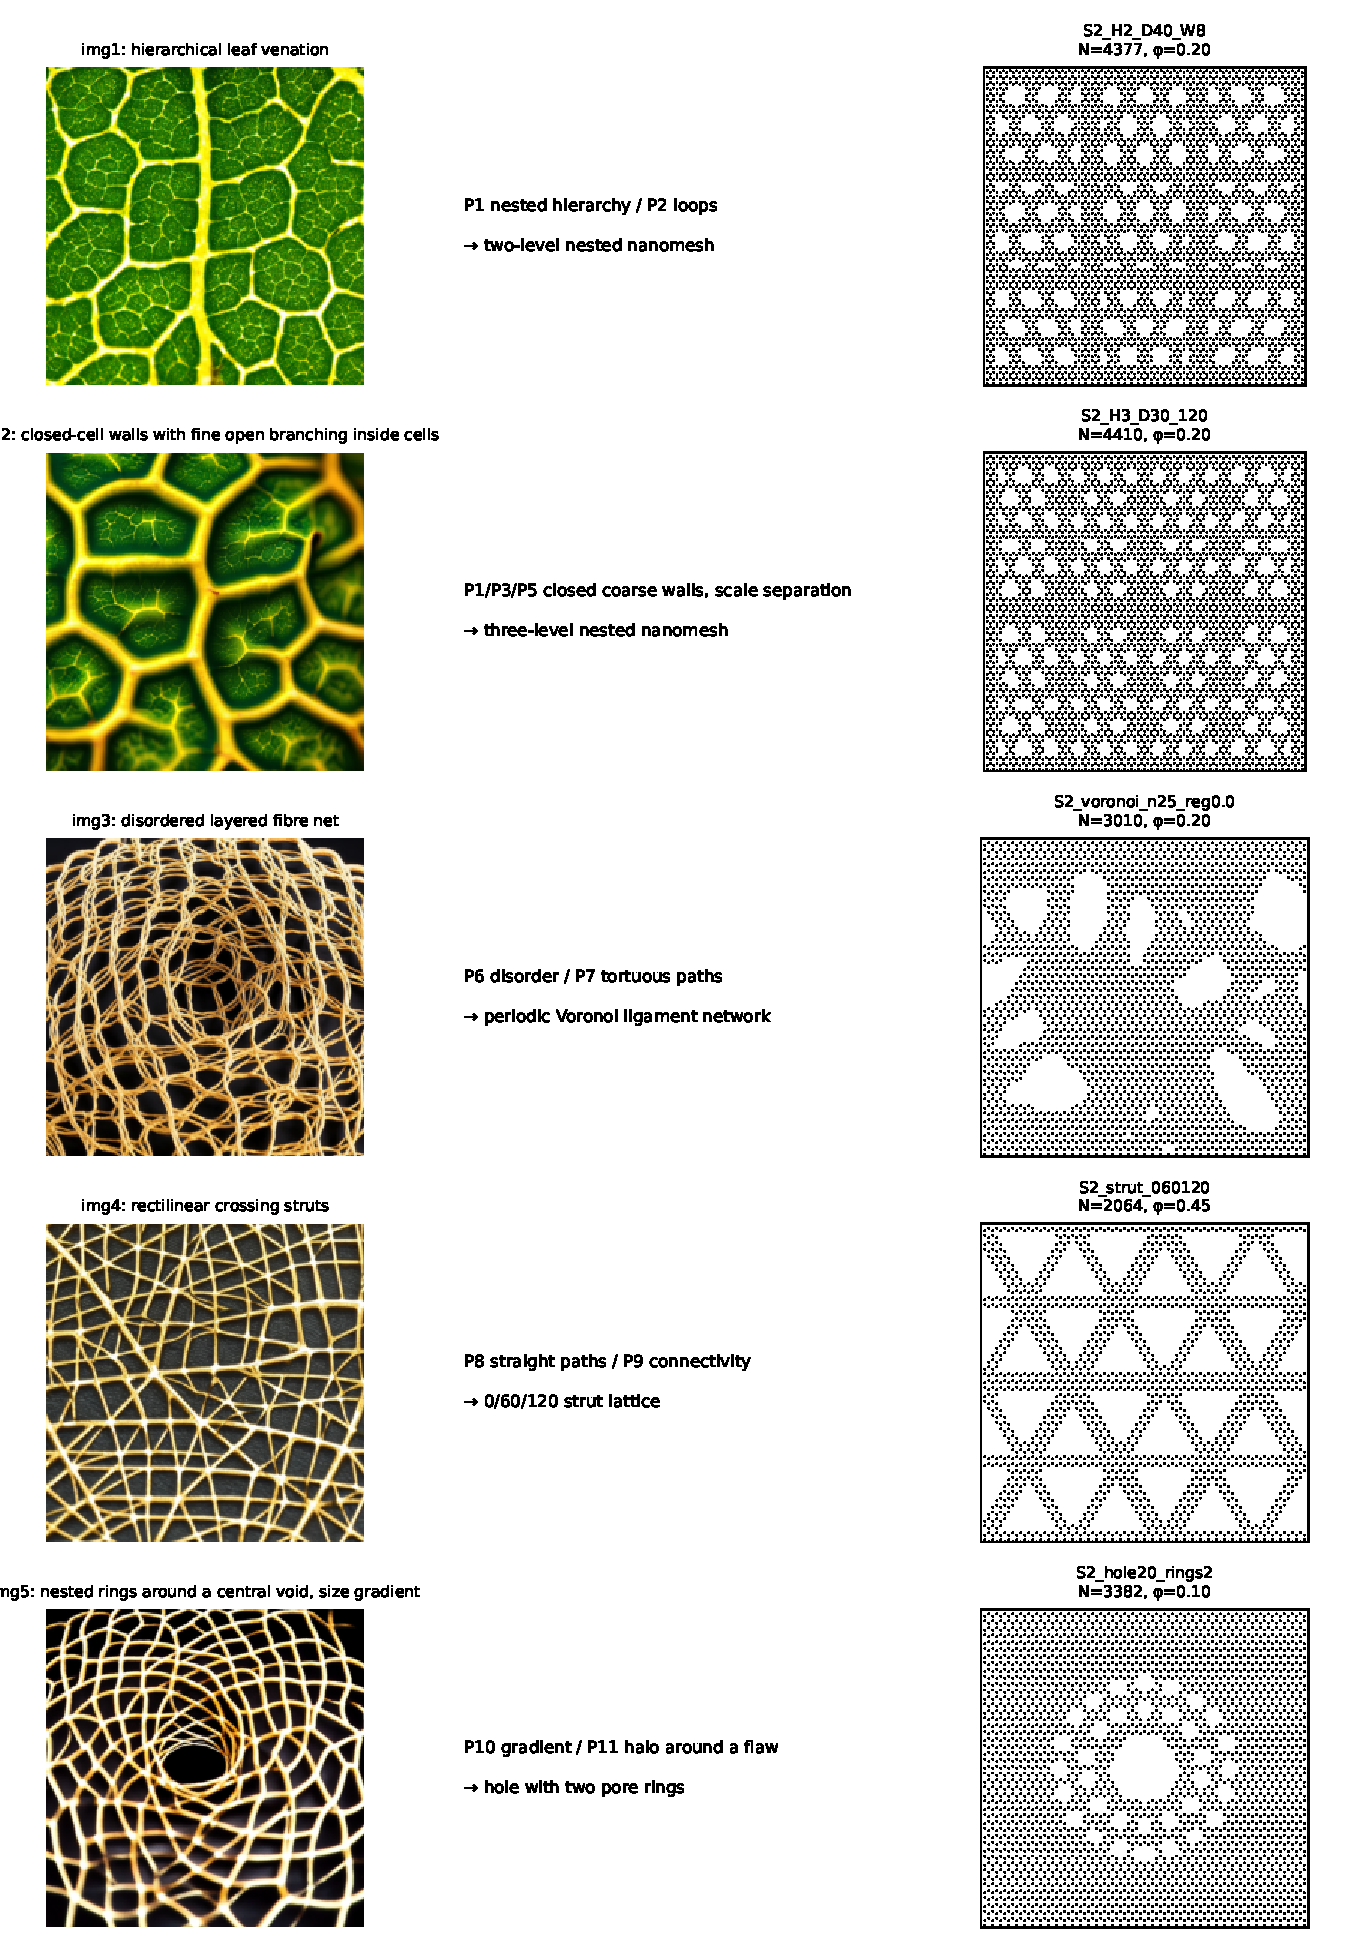
\includegraphics[width=0.9\textwidth]{design/translation.pdf}\caption{Translation from imagery to atomistic carbon architecture: each reference image (left) motivated one or more design principles (middle) that were instantiated as an explicit periodic graphene-derived structure (right; atoms shown as dots). The structures are not traced from the images; they realise the abstract principle with controlled parameters and matched porosity.}\label{fig:translation}\end{figure}
\begin{figure}[H]\centering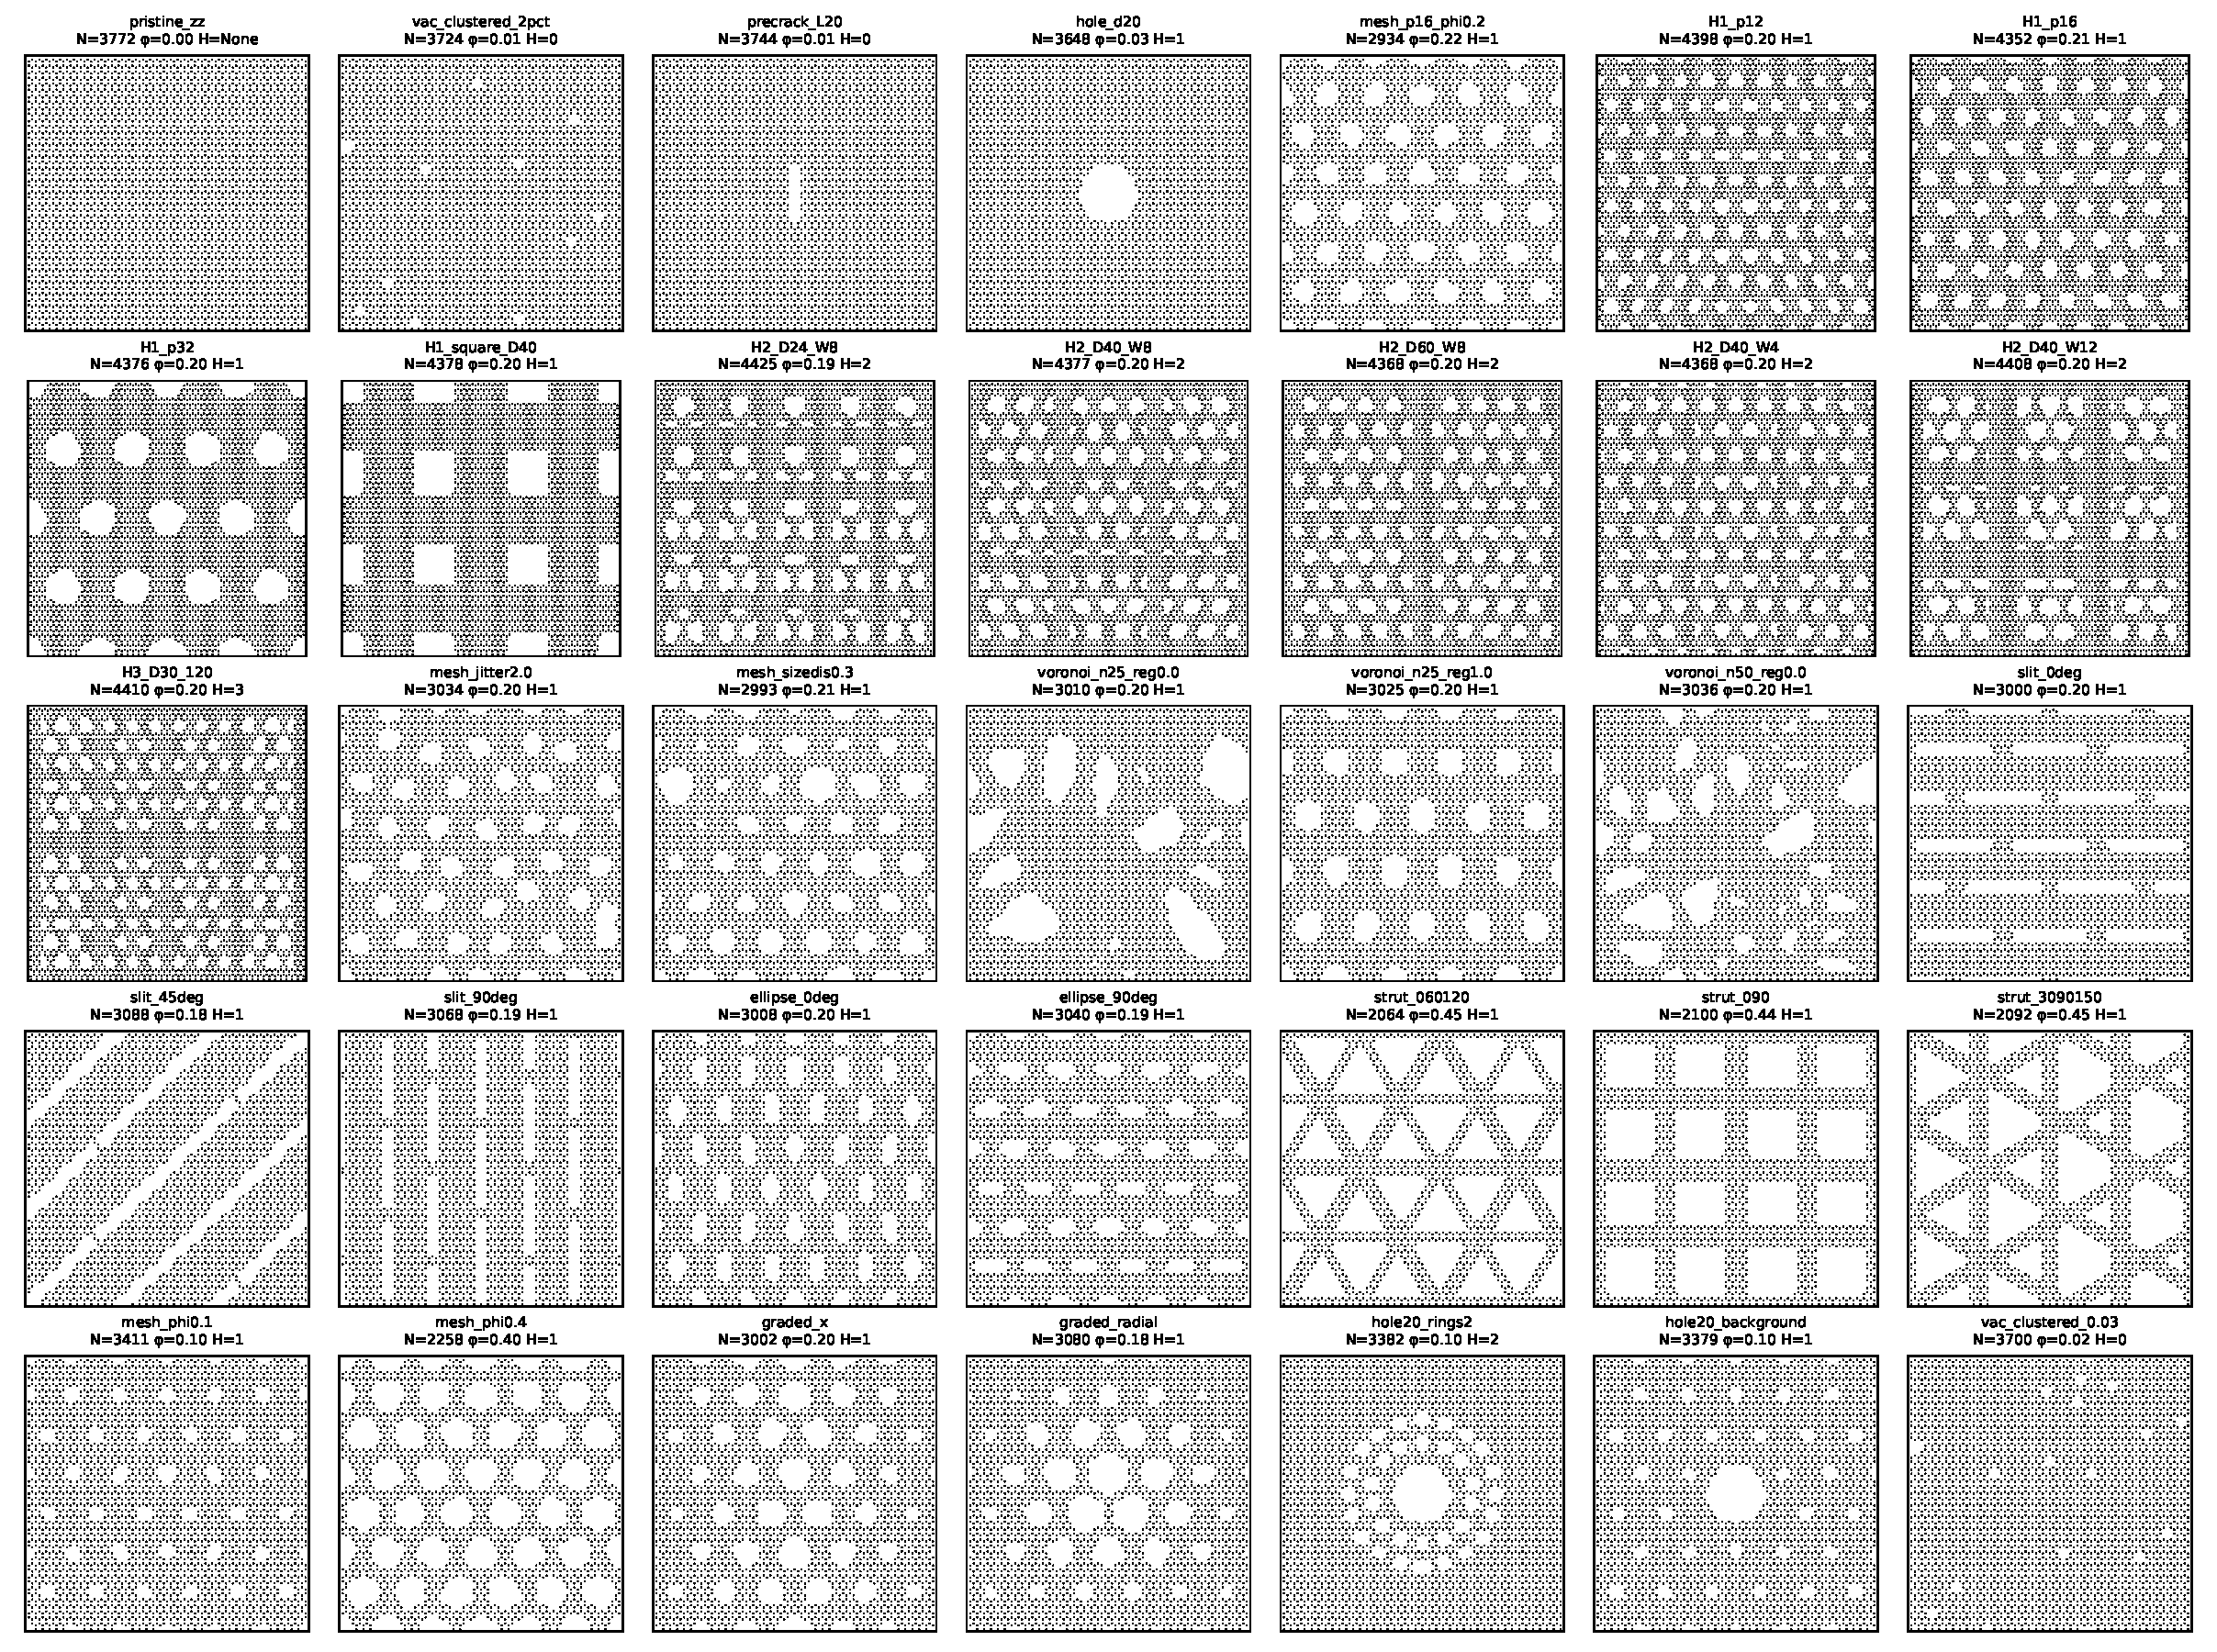
\includegraphics[width=1.0\textwidth]{design/design_space.pdf}\caption{The explored design space (Stages 1-2): baselines (pristine, vacancies, cracks, hole, reference mesh), the hierarchy ladder (single-scale meshes with three periods, coarse level alone, two-level meshes with three scale ratios and three vein widths, three-level mesh) at matched porosity 0.20, disorder (jitter, size dispersion, Voronoi networks of different regularity and cell count), anisotropy and load-path organisation (slits at 0/45/90 degrees, elliptical pores, strut lattices with and without a strut family along the load), porosity sweep, gradients, and flaw halos. N = atoms, phi = porosity, H = designed hierarchy depth. Loading is along x (horizontal).}\label{fig:space}\end{figure}
\section{Results}
\subsection{Stage 1: baselines}
Nine baselines (Fig.~\ref{fig:stage1}) anchor the design space. Pristine zigzag graphene (40\,\AA{} cell, homogeneous) reaches $\sigma_\mathrm{max}=38.8$\,N/m at 27\% strain and fails in a single avalanche; the dip in its curve near 18\% is the transverse-branch switch of the bistable homogeneous response discussed in Sec.~\ref{sec:validation}. Pristine armchair graphene peaks earlier and lower ($30.7$\,N/m at 18\%) and then softens continuously without bond loss until rupture at 30\% (the model's armchair response). The 2D modulus of all dense sheets is 224--250\,N/m ($287$\,N/m for armchair in the uniaxial-stress protocol), consistent with the elastic validation. Two per cent vacancies reduce the strength to $\approx24$\,N/m whether distributed (23.6\,N/m) or clustered (24.4\,N/m), but the fracture mode differs: distributed vacancies fail progressively (first bond loss at 9.8\%, peak at 12.8\%, failure at 14.3\%, six damage steps, load retained after the peak), while the clustered ones fail in one avalanche after a single first damage event. Central slit cracks of 10, 20 and 30\,\AA{} give 24.1, 18.5 and 18.7\,N/m; the 10$\to$20\,\AA{} step follows a Griffith-type power law (fitted exponent $-0.38$ against $-0.5$), but the 30\,\AA{} crack is \emph{not} weaker than the 20\,\AA{} crack: it starts to lose bonds at 7.9\% strain, grows stably bond by bond while the load still rises to 9.9\%, and only then runs. A circular hole of 20\,\AA{} (19.1\,N/m) is as damaging as a 20\,\AA{} crack. The reference nanomesh (period 16\,\AA, $\phi=0.22$) has $Y_{2D}=119$\,N/m, $\sigma_\mathrm{max}=12.0$\,N/m at 14\%, first damage at 10\% and fails progressively over 17\% strain with $W=1.1$\,J/m$^2$, i.e. it is 3$\times$ weaker than pristine graphene but retains load over a strain range comparable to the intact sheet's elastic range. Two features that recur later are already visible: (i) architecture changes the \emph{mode} of fracture at nearly constant strength (vacancy organisation), and (ii) sharp flaws beyond $\approx$20\,\AA{} enter a flaw-tolerant regime in this model, where stable crack growth precedes the instability.

\begin{figure}[H]\centering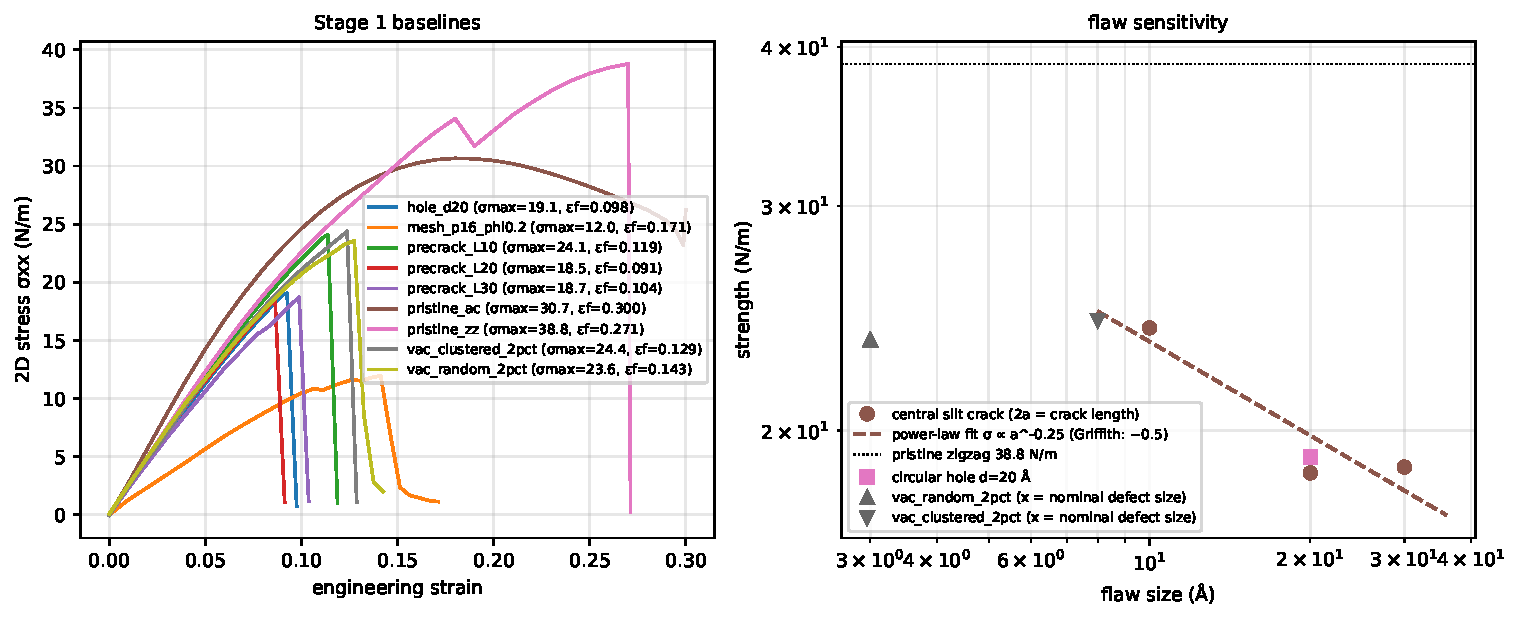
\includegraphics[width=1.0\textwidth]{campaign/stage1_baselines.pdf}\caption{Stage 1 baselines. Left: stress-strain curves of pristine zigzag/armchair graphene, distributed and clustered vacancies (2\%), central cracks of 10/20/30 A, a 20 A circular hole and the reference nanomesh. Right: strength versus flaw size for the cracks with a power-law fit (a Griffith-type scaling would give an exponent of -0.5), compared with the hole and the vacancy structures.}\label{fig:stage1}\end{figure}
\subsection{Stage 2: reconnaissance of the design variables}
Thirty-nine designs were simulated in Stage~2 (Figs.~\ref{fig:ss2}--\ref{fig:ladder}; all at matched porosity $\phi=0.20\pm0.02$ and identical footprint unless stated, uniaxial stress along $x$). The observations that drove the hypotheses of Sec.~\ref{sec:hyp} are the following.

\paragraph{Orientation and load-path organisation dominate.} Slit pores parallel to the load give $\sigma_\mathrm{max}=25.4$\,N/m and $W=3.3$\,J/m$^2$, slits at $45^\circ$ 18.5\,N/m, slits perpendicular to the load 4.0\,N/m -- a factor 6.4 at identical porosity. Elliptical pores elongated along the load reach 19.0\,N/m against 8.6\,N/m across the load. In the strut lattices ($\phi=0.45$) the $0/90^\circ$ lattice with a continuous strut family along the load (11.5\,N/m) beats the triangulated $0/60/120^\circ$ lattice (7.4\,N/m, which relaxes strongly and fails in one avalanche) and the $30/90/150^\circ$ lattice without any load-parallel strut (6.0\,N/m); node connectivity (six- vs four-connected nodes) is thus much less important than whether straight through-going ligaments exist along the load (principles P8/P9).

\paragraph{Hierarchy does not add strength.} On the hierarchy ladder the coarse single-scale meshes are strongest (square pores on the 40\,\AA{} grid 17.0\,N/m, round pores with a 32\,\AA{} period 16.4\,N/m), the fine single-scale meshes weakest (11.7--13.3\,N/m for 16 and 12\,\AA{} periods) and all nested two-level meshes lie in between (12.7--14.3\,N/m): strength grows with vein width (4/8/12\,\AA: 13.2/12.8/13.7) and decreases with domain size (24/40/60\,\AA: 14.3/12.8/12.7); the three-level mesh (13.0\,N/m) equals the fine mesh. Failure strain and work to failure of the nested meshes (0.14--0.26, 1.0--1.5\,J/m$^2$) do not exceed those of the single-scale meshes (0.13--0.26, 0.9--1.9\,J/m$^2$). What hierarchy does change is the mode: the coarse square mesh accumulates harmless corner damage from 13.5\% strain and then snaps all load-parallel ligaments together at 17\%, whereas the nested meshes lose their fine level first (first damage at 11--13\%), retain 20--60\% of the peak load on the load-parallel veins and fail through crack bands that channel along columns adjacent to the load-\emph{perpendicular} veins (Sec.~\ref{sec:top}).

\paragraph{Disorder is a two-channel variable.} Pore-position jitter of 1/2/3\,\AA{} changes strength only mildly (12.7/11.8/11.1 versus 11.7\,N/m ordered) while lengthening the failure strain from 0.13 to 0.21--0.24 and multiplying the number of discrete damage events (6 $\to$ 17--22); pore-size dispersion of 15/30\% gives 12.0/11.3\,N/m with the same tail elongation. In the polygonal Voronoi networks the dependence is non-monotonic: random seeds 8.2--9.7\,N/m, 60\% regularised 14.4\,N/m (the best network, $W=1.6$\,J/m$^2$), fully regular 13.3\,N/m -- the random networks contain a few thin, misoriented ligaments that act as weak links and localise the damage ($L=0.40$--$0.42$).

\paragraph{Porosity and lattice orientation.} For the reference mesh the strength falls as 19.6/11.7/9.4/7.3\,N/m for $\phi=0.1/0.2/0.3/0.4$; the net-section strength $\sigma_\mathrm{max}/(1-\phi)$ itself decreases (21.7 $\to$ 12.2\,N/m), so thinner ligaments are intrinsically weaker in this model. Rotating the graphene lattice so that the armchair direction carries the load changes the mesh strength by only 3\% (11.3 vs 11.7\,N/m), whereas it changes the pristine sheet by 21\%: the architecture, not the lattice chirality, controls the porous sheets.

\paragraph{Gradients and flaw halos.} A pore-size gradient along or radial to the load (10.1 and 10.0\,N/m) is worse than the uniform mesh at equal porosity because the largest pores form the weakest section. Around a 20\,\AA{} hole, two rings of 5\,\AA{} pores (16.2\,N/m) cost less strength than the same porosity spread uniformly in the far field (13.2\,N/m), but both are below the bare hole (19.1\,N/m): the halo does not shield the flaw, it only localises the penalty of the added porosity.

\paragraph{Defect organisation changes the mode, not the strength.} Random and clustered vacancies give 27.5/27.2\,N/m at 1\%, 23.6/24.4 at 2\% and 22.4/23.4 at 3\%; in every pair the distributed defects fail progressively (6--9 damage steps, load retained) and the clustered ones in a single avalanche.

\paragraph{A single descriptor explains most of the strength variation.} Across all 39 designs the strength is best organised by the minimum load-bearing solid fraction across the loading direction (Fig.~\ref{fig:maps}); the ratio $\sigma_\mathrm{max}/\mathrm{minSF}$ (a net-section strength) is 29--32\,N/m for straight, load-parallel ligaments (slits, square and round coarse pores, load-elongated ellipses), 17--19\,N/m for fine round-pore meshes with ligaments of 10--13\,\AA{}, 22\,N/m for the 32\,\AA{} round-pore mesh, and 12--15\,N/m for random networks. Neither porosity, ligament width, edge-atom fraction, anisotropy index nor tortuosity alone orders the data as well.

\begin{figure}[H]\centering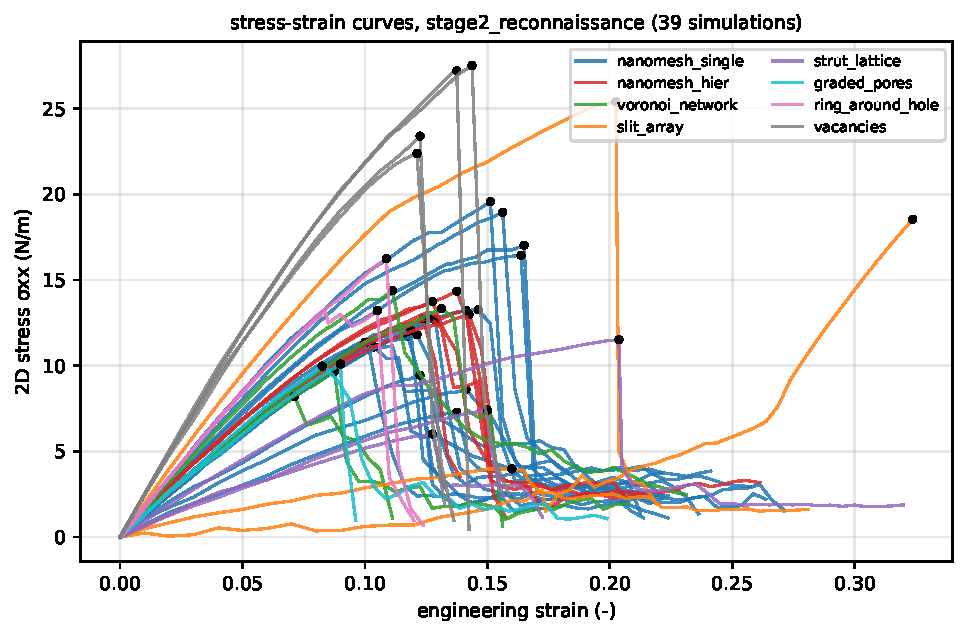
\includegraphics[width=0.85\textwidth]{campaign/stress_strain_stage2_reconnaissance.pdf}\caption{stress-strain curves, stage2\_reconnaissance (39 simulations). Every curve is an individual AQS simulation (uniaxial stress, REBO2+S); dots mark the peak stress.}\label{fig:ss2}\end{figure}
\begin{figure}[H]\centering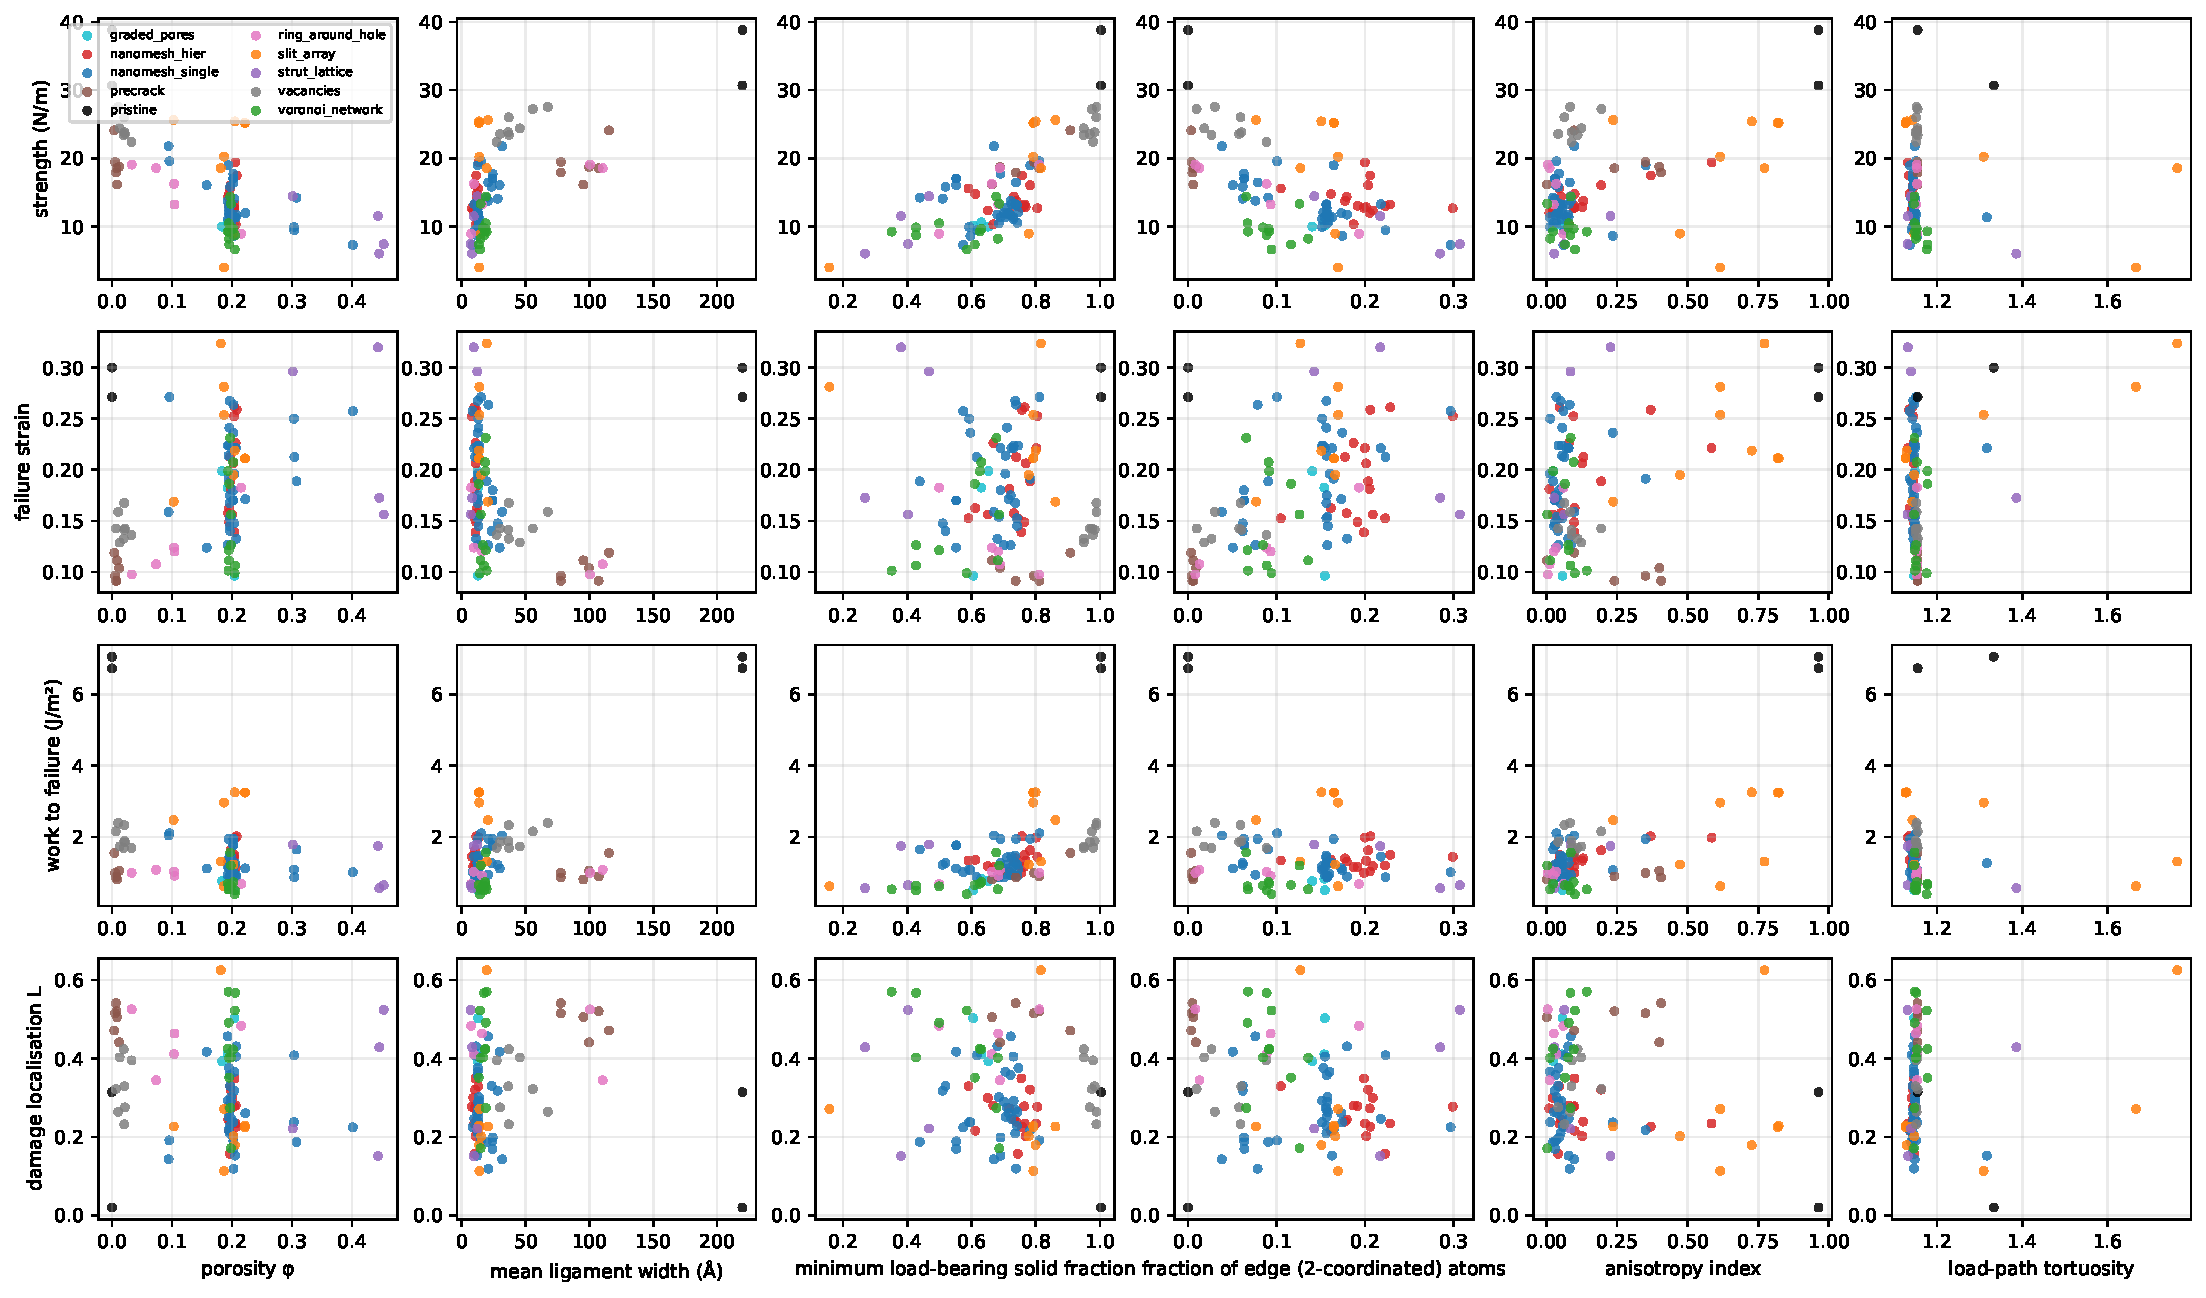
\includegraphics[width=1.0\textwidth]{campaign/property_maps.pdf}\caption{Structure-property maps of all completed simulations: strength, failure strain, work to failure and damage localisation as functions of measured structural descriptors (porosity, mean ligament width, minimum load-bearing solid fraction across the loading direction, fraction of two-coordinated edge atoms, anisotropy index and load-path tortuosity). Each point is one simulation; colours denote architecture families.}\label{fig:maps}\end{figure}
\begin{figure}[H]\centering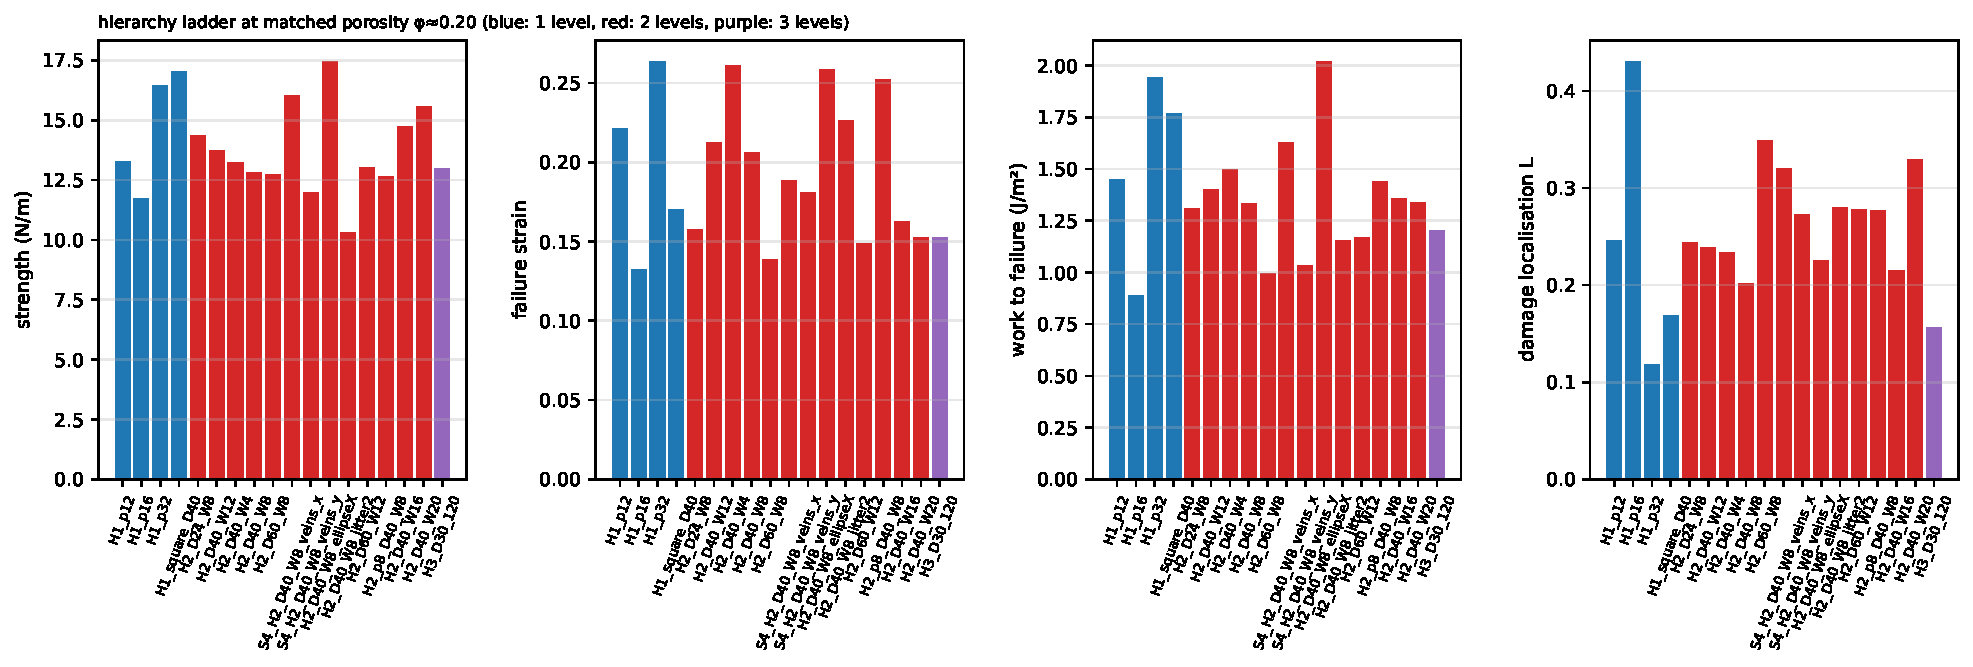
\includegraphics[width=1.0\textwidth]{campaign/hierarchy_ladder.pdf}\caption{Hierarchy ladder: mechanical metrics of single-scale nanomeshes (1 level: fine, reference and coarse periods; square coarse pores), two-level nested meshes with different domain sizes (scale ratios 2, 3.3, 5) and vein widths (4, 8, 12 A), and a three-level mesh, all at matched porosity (0.20 +- 0.01) and identical footprint.}\label{fig:ladder}\end{figure}
\subsection{Stage 3: competing hypotheses}
\label{sec:hyp}
\paragraph{H-A: Net section x load-path straightness controls strength} \textbf{Observation}: At matched porosity 0.20 the strength varies 6x (slit\_90 4.0, ellipse\_0 8.6, random Voronoi 8.2-9.7, fine meshes 11.7-13.3, coarse meshes 16.4-17.0, ellipse\_90 19.0, slit\_0 25.4 N/m). Dividing by the minimum load-bearing solid fraction across the loading direction (minSF) collapses the range to a 'net-section strength' of 12-32 N/m that is highest for straight, uniform-width ligaments parallel to the load (slit\_0 31.8, square mesh 31, p32 22) and lowest for necked/curved paths (round-pore meshes 17-19, random Voronoi 12). \textbf{Proposed mechanism}: sigma\_max = minSF x sigma\_0 / K, where sigma\_0 ~ 39 N/m is the intrinsic strength and K is a geometric knockdown set by the curvature/necking of the load-bearing ligaments (K ~ 1.2 straight strips, ~2 necked round-pore ligaments, ~3 random networks); hierarchy and porosity act only through minSF and K. \textbf{Competing explanation}: H-B: strength is controlled by the fraction of under-coordinated edge atoms (atomic-scale edge weakness), not by continuum stress concentration; at fixed minSF, strength decreases with edge-atom fraction and is insensitive to ligament shape. \textbf{Predicted if mechanism holds}: A coarse square-pore mesh and a coarse round-pore mesh with the same minSF (pore width = square side) have square $>$= round (straight strips beat necked paths) despite more edge atoms in the square; strength of any new design is predicted within ~20\% by minSF x 31/K. \textbf{Predicted if competing explanation holds}: Round $>$= square at equal minSF (fewer edge atoms), and designs with equal edge-atom fraction but different ligament straightness (slit\_0 vs jittered mesh, both fUC ~0.15) would have similar strength -- they differ 2x, so H-B is already disfavoured. \textbf{Discriminating experiments}: S4 pair 1: square vs circle coarse mesh at equal minSF and equal period; S4 pair 2: same at equal porosity; S5: vein-width sweep of nested meshes (rule of mixtures of straight veins and necked fine ligaments). \textbf{Outcome}: PARTLY REFUTED (Stage 4 pairs 1-2): at equal net section, circular coarse pores are as strong as square ones (16.1 vs 17.0 N/m; predicted 11.3), and at equal porosity 14.1 (predicted 9.8): the pore shape does not matter at the coarse scale, so the 'necking knockdown' of H-A is wrong. The net-section factor itself is confirmed (slit\_0 at porosity 0.1 and 0.2: 25.6 vs 25.4 N/m; vein-width series). REVISED (H-A'): sigma = minSF x sigma\_net, where sigma\_net depends on the absolute ligament width (edge/discreteness effect, ~17 N/m for 10-13 A ligaments, 22-31 N/m for $>$= 18 A) and on load-path alignment (random networks 12-15 N/m), not on pore shape. Edge-atom fraction (H-B) explains the size dependence but not the orientation effects.

\paragraph{H-C: Fracture mode is set by the equivalence of parallel load paths} \textbf{Observation}: Perfectly periodic straight-ligament structures fail in one avalanche (square mesh: 6 harmless corner events then all rows snap at 17.0 N/m; slit\_0: stepwise with 3 events; clustered vacancies), whereas structures whose load-bearing paths are non-equivalent (fine round-pore meshes 15-22 events, jittered meshes 17-22, nested meshes 15-16, distributed vacancies 9) fail progressively with post-peak load retention. \textbf{Proposed mechanism}: When all load-bearing ligaments are crystallographically equivalent they reach the instability at the same strain and snap together (no load transfer possible); necking, disorder or hierarchy make ligaments non-equivalent so they fail sequentially and the surviving ones carry the transferred load. \textbf{Competing explanation}: H-C': the mode is set by the ligament shape alone (straight = abrupt, necked = progressive) irrespective of equivalence. \textbf{Predicted if mechanism holds}: Introducing +-15\% dispersion of the ligament widths into the square coarse mesh (same porosity) converts the single avalanche into a multi-step failure at nearly the same peak stress; a perfectly uniform fine mesh remains progressive only because of necking. \textbf{Predicted if competing explanation holds}: The dispersed square mesh still fails in one avalanche. \textbf{Discriminating experiments}: S4 pair 3: square mesh with size dispersion 0.15 vs ordered; S4 pair 4: p32 round mesh with and without dispersion. \textbf{Outcome}: REFUTED (Stage 4 pairs 3-4): +-15\% ligament dispersion lowered the strength of both coarse meshes (17.0 -$>$ 15.8; 16.4 -$>$ 13.8) and did not make failure progressive (square: still a single avalanche; p32: shorter, more localised failure, L 0.12 -$>$ 0.46). Load-path non-equivalence is not sufficient; a fibre-bundle-type criterion applies: sequential failure requires enough parallel paths that the load transferred by one failing path stays below the strength margin of the others. Fine meshes (8-10 rows) and jittered meshes satisfy it, three wide strips do not.

\paragraph{H-D: Disorder trades strength for progressivity with an optimum for energy absorption} \textbf{Observation}: Pore-position jitter 0/1/2/3 A gives 11.7/12.7/11.8/11.1 N/m but failure strains 0.13/0.21/0.24/0.22 and 6/17/22/21 damage steps; Voronoi regularity 0/0.6/1 gives 9.7/14.4/13.3 N/m and W 0.74/1.56/1.20 J/m2 (n25); random n50 8.2 N/m. \textbf{Proposed mechanism}: Disorder acts through two opposing channels: it creates weak links (thin or misoriented ligaments) that lower the peak (extreme-value control), and it breaks the equivalence of load paths so that failure becomes sequential (longer tail, more work). The net effect on work to failure is positive at moderate disorder and negative when weak links dominate. \textbf{Competing explanation}: H-D': disorder always lowers both strength and work (pure weak-link picture); or disorder always raises work (pure crack-path-disruption picture). \textbf{Predicted if mechanism holds}: W(disorder) is non-monotonic with a maximum at intermediate disorder for both jittered meshes and Voronoi networks; seed-to-seed scatter of strength grows with disorder. \textbf{Predicted if competing explanation holds}: W monotonically decreasing (weak link) or increasing (disruption). \textbf{Discriminating experiments}: S5: Voronoi regularity sweep 0/0.3/0.6/0.8/1.0; S6: 3 seeds each for jitter 2 A, size dispersion 0.15, Voronoi reg 0.0 and 0.6; lattice-registry replicates of the ordered mesh. \textbf{Outcome}: PARTLY SUPPORTED, seed statistics decisive (Stages 5-6): jitter trades a mild strength loss (12.7 -$>$ 11.1 N/m) for longer tails, but seed replicates show large scatter of the post-peak tail (jitter 2 A: failure strain 0.24 vs 0.15 between seeds). In Voronoi networks the apparent optimum at regularity 0.6 (14.4 N/m) was a single-seed effect (seed 2: 9.2 N/m); regularity 0.3/0.8 give 10.5/6.6 N/m and random seeds 8.7-9.7 N/m: strength of random networks is controlled by the weakest ligament (extreme-value statistics), not by regularity, and work does not show a robust optimum. Lattice-registry replicates of the ordered mesh (11.7/12.0/13.1/13.1/13.3 N/m) show that the atomic placement of pore edges alone moves strength by ~12\% and can switch the mode (abrupt vs progressive), setting the resolution of all fine-mesh comparisons.

\paragraph{H-E: Flaw tolerance beyond ~20 A: crack-tip lattice trapping caps the size effect} \textbf{Observation}: Cracks of 10/20/30 A give 24.1/18.5/18.7 N/m (Griffith scaling would give 24.1/17.0/13.9); the 30 A crack starts breaking bonds at 7.9\% strain and grows stably to 9.9\% before running; a 20 A hole (19.1) equals a 20 A crack. \textbf{Proposed mechanism}: In this discrete lattice the crack advances by discrete bond-breaking events with an energy barrier (lattice trapping); once the flaw exceeds a few nanometres the peak stress is set by the trapping strength of the tip bond configuration rather than by the flaw length. \textbf{Competing explanation}: H-E': the plateau is a periodic-image artefact (30 A crack in a 100 A cell interacts with its images) and strength keeps decreasing with crack length in larger cells. \textbf{Predicted if mechanism holds}: A 40 A crack in a 150 A cell and a 30 A crack in a 150 A cell both give 17-19 N/m; a 30 A hole gives ~18 N/m. \textbf{Predicted if competing explanation holds}: Strength continues to fall (40 A: ~13 N/m in the large cell). \textbf{Discriminating experiments}: S4: precrack 30/40 A in 150 A cells; hole 30 A. \textbf{Outcome}: SUPPORTED (Stage 4): 30 A and 40 A cracks in 150 A cells give 19.5 and 17.9 N/m (predicted 17-19; Griffith scaling 13.9 and 12.0), a 30 A hole 18.6 N/m (20 A hole 19.1). Beyond ~20 A the strength of a flawed sheet is set by the trapping strength of the tip bond configuration (stable bond-by-bond growth precedes the instability), not by the flaw length; the plateau is not a periodic-image artefact.

\paragraph{H-F: Nested hierarchy does not add strength; the finest load-bearing level and the load-parallel veins control it} \textbf{Observation}: Two-level meshes (12.7-14.3) lie between the fine (11.7-13.3) and coarse (16.4-17.0) single-scale limits at matched porosity; strength rises with vein width (W4/8/12: 13.2/12.8/13.7) and falls with domain size (D24/40/60: 14.3/12.8/12.7); the three-level mesh (13.0) equals the fine mesh. Fracture panels show the fine level failing first at pore edges, load-parallel veins carrying the residual load, and cracks channelling along columns next to load-perpendicular veins. \textbf{Proposed mechanism}: The nested structure is a parallel arrangement of straight veins (strong, straight strips) and a necked fine mesh (weak); the fine level reaches its instability first, the veins then carry a fraction W/D of the net section; perpendicular veins act as compliant crack channels rather than crack arrestors. \textbf{Competing explanation}: H-F': veins arrest cracks (compartmentalisation) so that nested meshes gain failure strain and work relative to single-scale meshes of equal strength. \textbf{Predicted if mechanism holds}: Veins along the load only (vein\_dirs='x') give higher strength than veins in both directions at equal porosity, and veins perpendicular only ('y') give no more than the fine mesh; the work to failure of nested meshes does not exceed that of the fine mesh with the same porosity. \textbf{Predicted if competing explanation holds}: xy veins beat x-only veins (compartments) and nested meshes have larger work than single-scale meshes. \textbf{Discriminating experiments}: S5: vein direction x / y / xy at matched porosity; vein width sweep to W = 20 A; hierarchy x disorder and hierarchy x anisotropy interactions. \textbf{Outcome}: SUPPORTED and sharpened (Stage 4-5): veins only along the load give 16.1 N/m and the largest work of the nested family (1.6 J/m2), veins in both directions 12.8, veins only perpendicular 12.0 = fine mesh; the vein-width series 4/8/12/16/20 A (13.2/12.8/13.7/14.8/15.6 N/m) approaches the coarse-only limit (17.0) monotonically and the mode turns abrupt at 20 A. Hierarchy adds strength only through load-parallel coarse ligaments; perpendicular veins are dead weight and act as crack channels rather than crack arrestors (H-F' rejected). Stage 5 additions: scale ratio at fixed vein geometry does not matter (period-8 fine level 12.7 vs period-12 12.8 N/m); D60/W12 13.0; jittering the fine level costs 2.5 N/m (12.8 -$>$ 10.3); elongating the fine pores along the load inside the nested mesh gives 17.5 N/m with W = 2.0 J/m2 and progressive failure -- the only interaction that beats the coarse-only limit (17.0, abrupt), because it combines straight fine ligaments (high net-section strength) with many parallel paths (fibre-bundle progressivity).
Five competing hypotheses were formulated from the Stage~1--2 observations before any further simulation (file \texttt{experiments/predictions/hypotheses.json}, with the observation, mechanism, competing explanation, and the observables predicted under each). They are listed below together with their outcome after Stages~4--6; the discriminating experiments themselves are described in the next subsection.

\subsection{Stage 4: discriminating experiments}
Ten matched-pair simulations were designed to separate the hypotheses; their quantitative predictions (strength and fracture-mode class) were written to a hashed file before launch (\texttt{experiments/\allowbreak predictions/\allowbreak stage4\_\allowbreak predictions.json}) and are compared with the outcomes in Fig.~\ref{fig:discriminating_experiments}. Median absolute error of the strength predictions: 6.5\% (mean 10\%, maximum 30\%); fracture-mode class correct in 8 of 10 cases.

\paragraph{Pore shape at equal net section (H-A vs H-B).} Circular coarse pores whose diameter equals the side of the square pores (same minimum solid fraction 0.51, lower porosity) reach 16.1\,N/m, statistically indistinguishable from the square mesh (17.0 in Stage~2, 17.0 in the re-run of the same design), while H-A's necking knockdown had predicted 11.3\,N/m; at equal porosity the round pores give 14.1\,N/m (predicted 9.8) because the net section falls to 0.50. The shape of coarse pores therefore does not matter; the knockdown observed for fine meshes is an absolute ligament-size effect (ligaments of 10--13\,\AA{} carry a net-section stress of 17--19\,N/m, ligaments of 18--24\,\AA{} 22--31\,N/m). H-A is revised accordingly (H-A$'$: net section times a size- and alignment-dependent net-section strength); H-B explains the size dependence but not the orientation effects.

\paragraph{Ligament dispersion (H-C).} Dispersing the pore sizes by $\pm15\%$ lowered the strength of the square coarse mesh from 17.0 to 15.8\,N/m without changing its single-avalanche mode, and lowered the 32\,\AA{} round-pore mesh from 16.4 to 13.8\,N/m while \emph{shortening} its post-peak tail (failure strain 0.26 $\to$ 0.13, localisation 0.12 $\to$ 0.46). H-C is refuted: making parallel load paths non-equivalent is not sufficient for progressive failure. The pattern is that of an equal-load-sharing fibre bundle: when a strip fails, its load is transferred to the remaining ones, and with only three wide strips (or with a weakest link that is much weaker than the rest) the transfer exceeds their margin and the failure cascades; fine meshes with 8--10 rows of small ligaments, and jittered meshes, stay below that threshold and fail sequentially.

\paragraph{Flaw-size plateau (H-E).} A 30\,\AA{} and a 40\,\AA{} crack in 150\,\AA{} cells give 19.5 and 17.9\,N/m (predicted 17--19; Griffith scaling from the 10 and 20\,\AA{} cracks would give 13.9 and 12.0), and a 30\,\AA{} hole gives 18.6\,N/m (20\,\AA{} hole: 19.1). The plateau is real and not a periodic-image artefact: in this discrete lattice the tip bond configuration and its trapping strength, not the flaw length, set the instability once the flaw exceeds a few nanometres.

\paragraph{Vein direction (H-F).} With the same porosity and fine level, veins only along the load give 16.1\,N/m and $W=1.6$\,J/m$^2$, veins in both directions 12.8\,N/m, and veins only across the load 12.0\,N/m -- the value of the fine mesh alone. Load-perpendicular veins are dead weight (they are not crack arrestors, H-F$'$ rejected), and the strength of a nested mesh is that of its finest level plus the contribution of the load-parallel coarse ligaments, as H-F predicted (14.5 and 11.5). The load-parallel-only design is also the only nested mesh that combines a strength close to the coarse-only limit with progressive failure.

\begin{figure}[H]\centering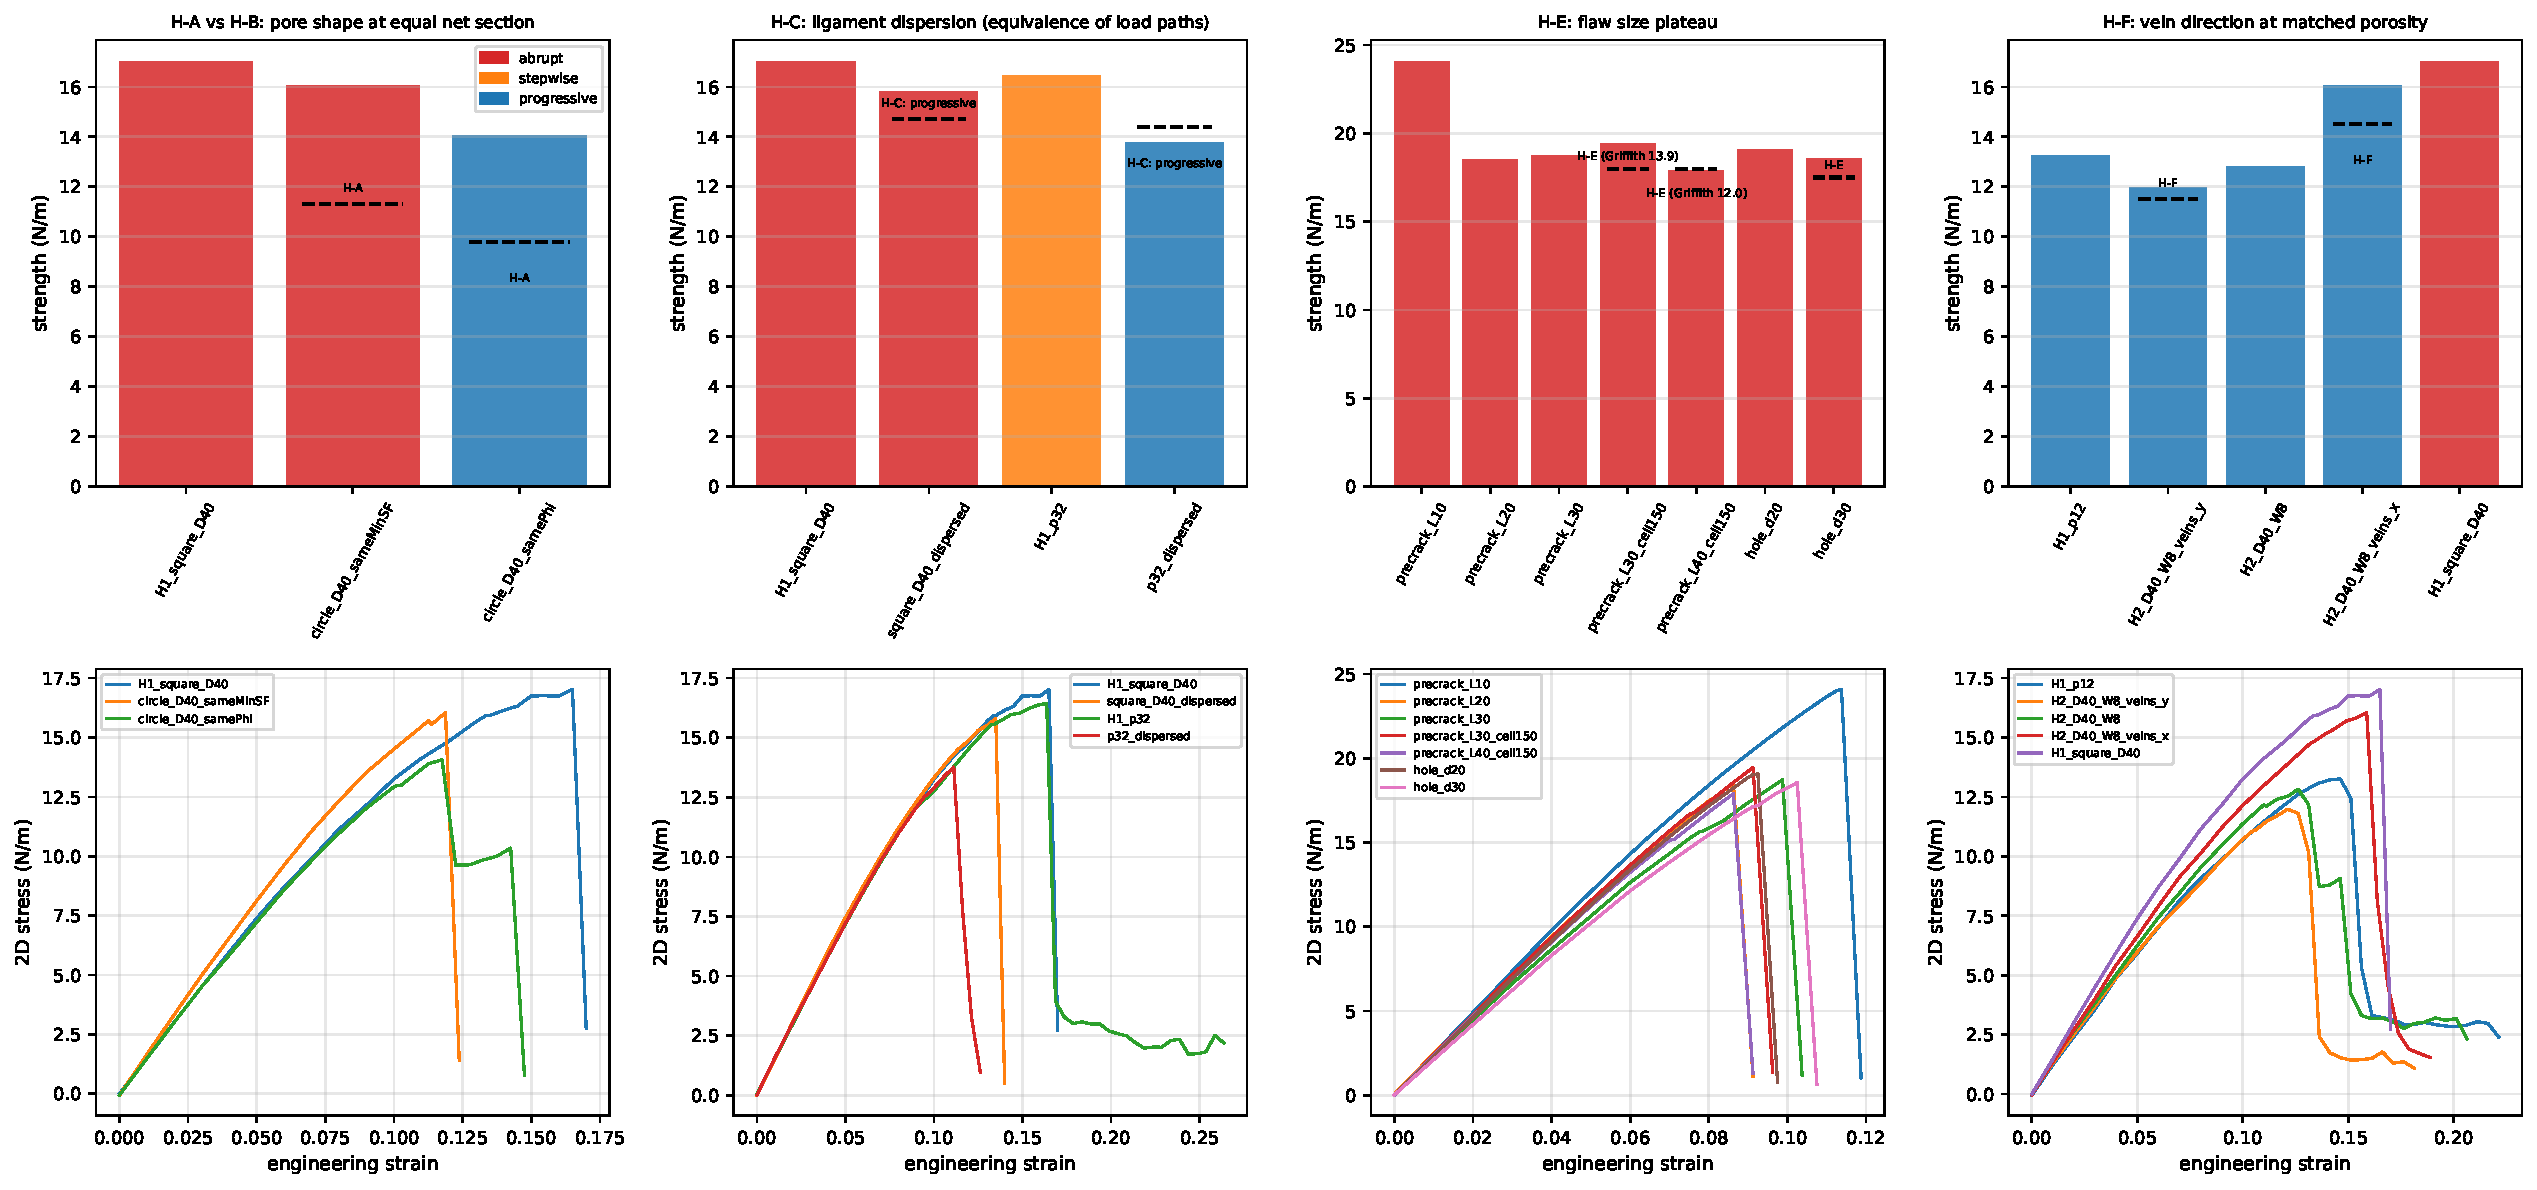
\includegraphics[width=1.0\textwidth]{campaign/discriminating_experiments.pdf}\caption{Stage 4 discriminating experiments. Top: observed strengths (bar colour = fracture mode) with the predictions recorded before the runs (dashed lines, labelled by the hypothesis that generated them); bottom: the corresponding stress-strain curves. Left to right: pore shape at equal net section (H-A vs H-B), ligament-width dispersion (H-C), flaw-size plateau in 100 and 150 A cells (H-E), vein direction in the nested mesh (H-F).}\label{fig:discriminating_experiments}\end{figure}
\subsection{Stage 5: deep mechanism studies (hierarchy, scaling, interactions)}
Thirteen further simulations mapped the variables that Stages~2 and 4 had identified as controlling (Figs.~\ref{fig:deep_hierarchy}--\ref{fig:deep_scaling}).

\paragraph{Vein width, scale ratio and inter-level interactions.} At matched porosity the strength of the two-level mesh rises monotonically with the width of its veins, 13.2/12.8/13.7/14.8/15.6\,N/m for $W=4/8/12/16/20$\,\AA, toward the coarse-only limit (17.0\,N/m), and the mode turns from progressive to abrupt at $W=20$\,\AA{} when the fine pores have shrunk to a few atoms; work to failure stays at 1.3--1.5\,J/m$^2$ throughout. The scale ratio at fixed vein geometry has no effect (fine period 8 vs 12\,\AA: 12.7 vs 12.8\,N/m), and a larger domain with wider veins (60/12\,\AA) gives 13.0\,N/m. Disordering the fine level costs the nested mesh the same 2--3\,N/m it costs a single-scale mesh (12.8 $\to$ 10.3). The single favourable interaction is hierarchy $\times$ anisotropy: elongating the fine pores along the load inside the nested mesh gives 17.5\,N/m, $W=2.0$\,J/m$^2$ and progressive failure with 0.26 failure strain -- the only nested design that exceeds the coarse-only mesh, because it combines straight fine ligaments (net-section strength close to the intrinsic value) with many parallel load paths (sequential failure).

\paragraph{Disorder.} The Voronoi regularity sweep (0/0.3/0.6/0.8/1.0: 9.2$\pm$0.5, 10.5, 11.2$\pm$2.8, 6.6, 13.3\,N/m) has no monotonic trend once the seed scatter is taken into account; only the fully regular (hexagonal-seed) network is reproducibly strong. The random networks fail from their thinnest ligament (localisation $L\approx0.4$--0.6), which is why their net-section strength (12--20\,N/m) lies below that of ordered meshes of the same ligament width (Fig.~\ref{fig:deep_scaling}, right).

\paragraph{Porosity scaling and the net-section rule.} For load-parallel slits the strength is independent of porosity (25.6/25.4/25.2\,N/m for $\phi=0.10/0.20/0.22$; the slit family cannot exceed $\phi\approx0.22$ at 4\,\AA{} slit width, so the two nominal 0.3/0.4 members are replicates of the 0.22 design and reproduced it exactly), because lengthening the slits does not change the net section perpendicular to the load. The square coarse mesh follows $\sigma\approx31\times\mathrm{minSF}$ (21.8/17.0/14.2\,N/m at $\phi=0.1/0.2/0.3$), whereas the fine round-pore mesh follows the lower line $\sigma\approx17\times\mathrm{minSF}$ (19.6/11.7/9.4/7.3\,N/m at 0.1--0.4) with its net-section strength itself decreasing as the ligaments thin. Across all porous designs the net-section strength is 45--55\% of the intrinsic strength for ligaments of 10--13\,\AA, 70--85\% for 25--30\,\AA, with load-parallel slits at the top and random networks scattered below (master plot).

\begin{figure}[H]\centering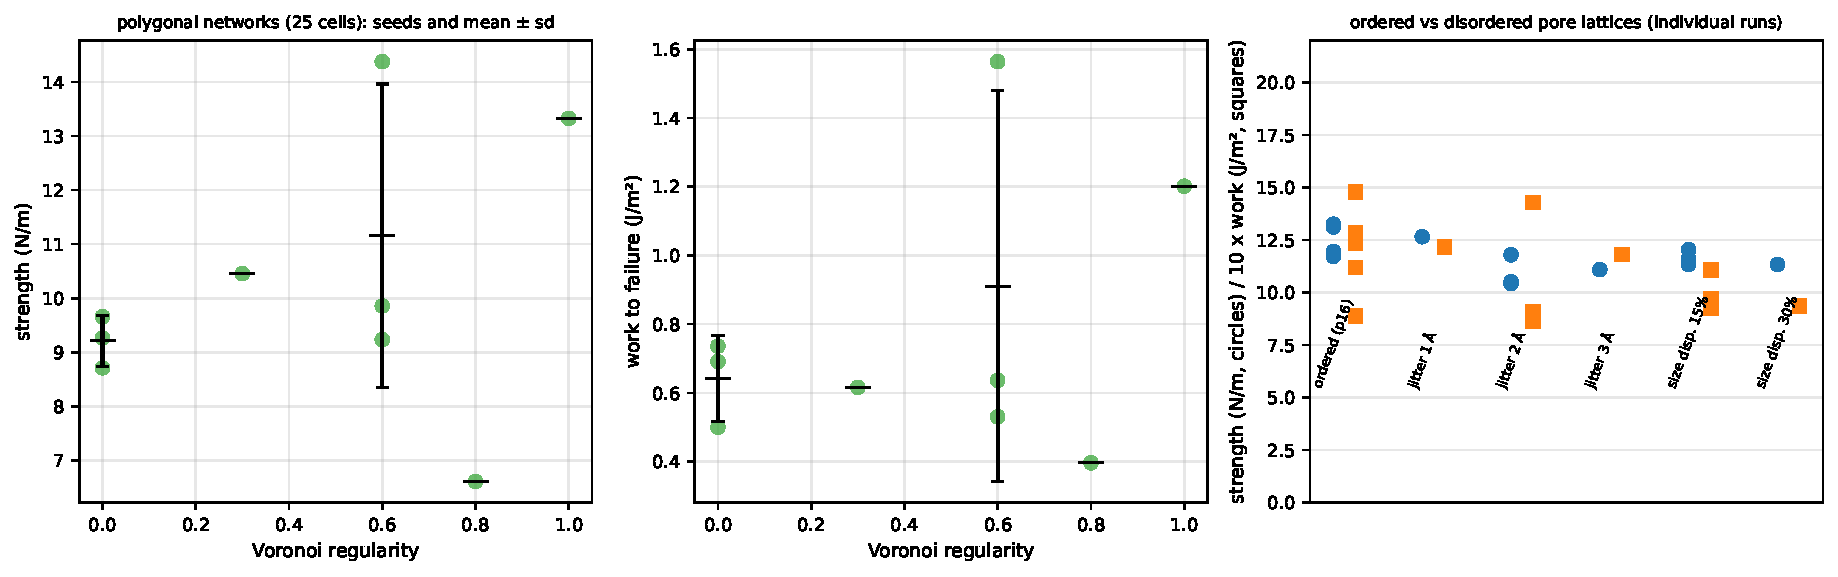
\includegraphics[width=1.0\textwidth]{campaign/deep_disorder.pdf}\caption{Deep study of disorder. Left/middle: strength and work to failure of periodic Voronoi networks versus seed regularity (dots: individual seeds; black: mean ± standard deviation). Right: individual runs of the ordered reference mesh (including lattice-registry replicates) and of jittered / size-dispersed meshes.}\label{fig:deep_disorder}\end{figure}
\begin{figure}[H]\centering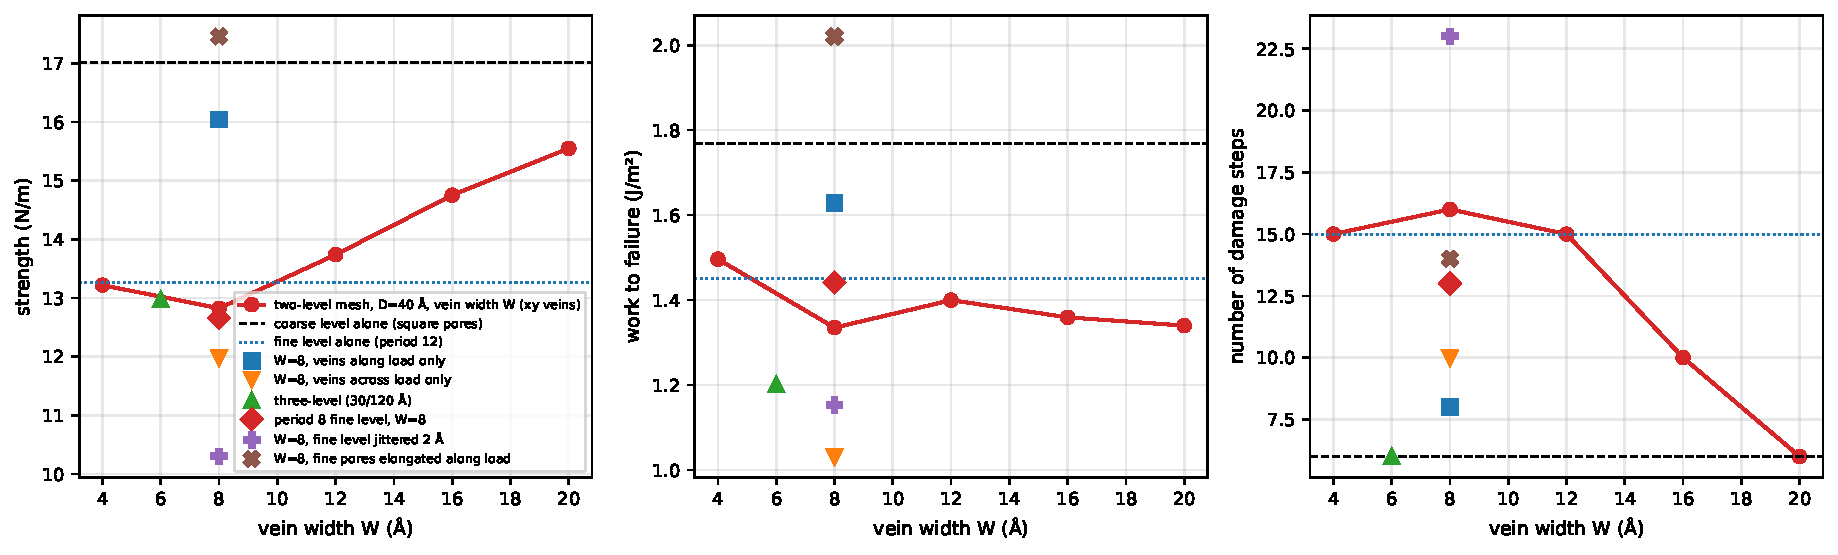
\includegraphics[width=1.0\textwidth]{campaign/deep_hierarchy.pdf}\caption{Deep study of hierarchy at matched porosity 0.20: strength, work to failure and number of discrete damage events versus vein width of the two-level mesh (red), compared with the coarse level alone (dashed), the fine level alone (dotted), the vein-direction variants (veins only along / only across the load), the three-level mesh, a finer fine level (period 8), and the hierarchy x disorder and hierarchy x anisotropy interactions.}\label{fig:deep_hierarchy}\end{figure}
\begin{figure}[H]\centering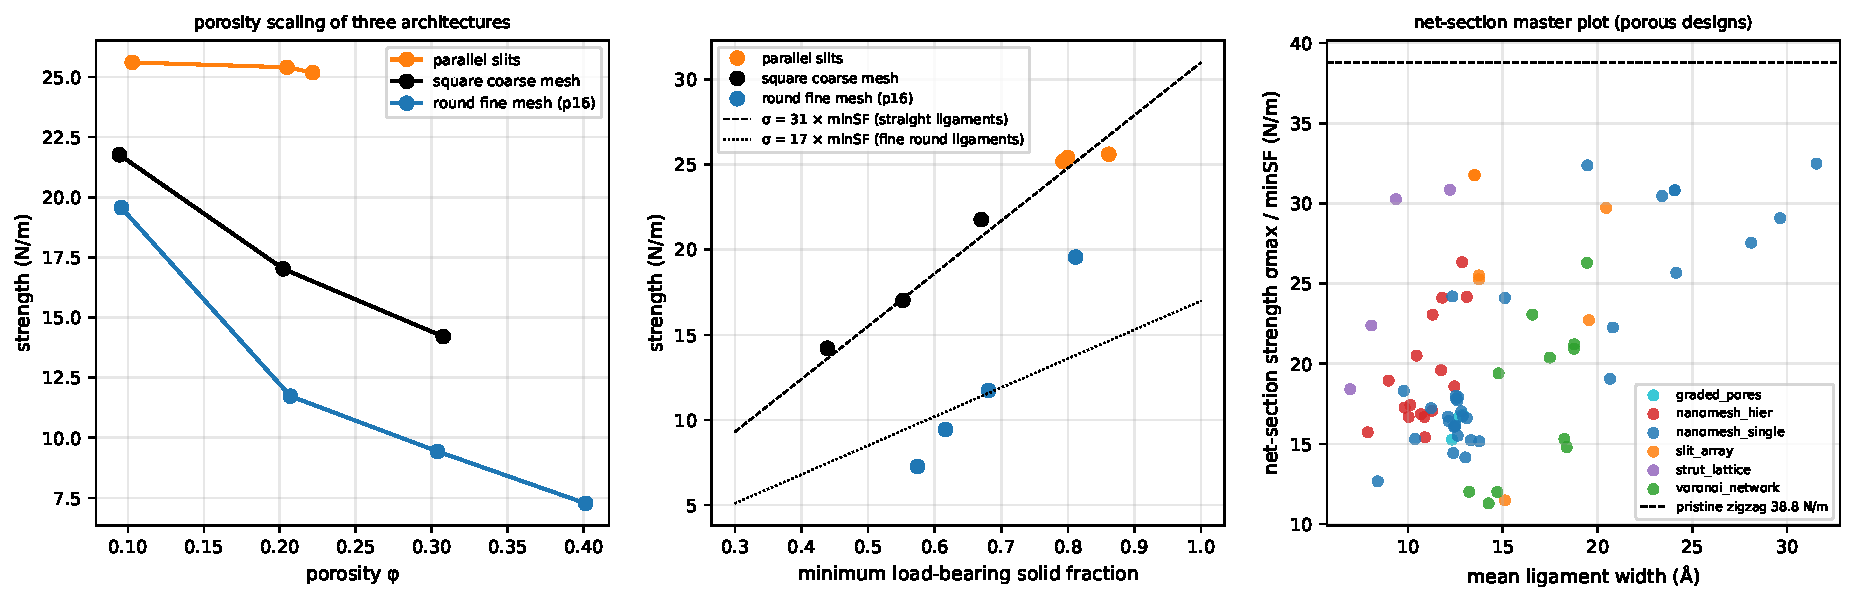
\includegraphics[width=1.0\textwidth]{campaign/deep_scaling.pdf}\caption{Scaling and the net-section rule. Left: strength versus porosity for parallel slits (whose net section is set by the slit width, not the slit length), the square coarse mesh and the round fine mesh. Middle: the same data versus the measured minimum load-bearing solid fraction with the two net-section lines. Right: net-section strength (strength divided by minimum solid fraction) versus mean ligament width for all porous designs; straight load-parallel ligaments approach the pristine strength, fine round-pore and random networks fall well below it.}\label{fig:deep_scaling}\end{figure}
\subsection{Stage 6: seed statistics}
Every stochastic architecture that entered a conclusion was replicated with three independent seeds (Fig.~\ref{fig:seeds}; individual values in the database). The distributed 2\% vacancies give $24.5\pm1.3$\,N/m and $W=2.0\pm0.3$\,J/m$^2$; the size-dispersed mesh $11.7\pm0.4$\,N/m; the jittered mesh $10.9\pm0.8$\,N/m with failure strains of 0.15/0.15/0.24, i.e. the long post-peak tail of the first seed was not typical; the random Voronoi networks $9.2\pm0.5$\,N/m; and the 60\%-regularised Voronoi networks $11.2\pm2.8$\,N/m (9.2/9.9/14.4) -- the best network of Stage~2 was a single-seed outlier, and the apparent optimum at intermediate regularity does not survive replication (regularity 0.3/0.8 give 10.5/6.6\,N/m). The random networks are thus consistently the weakest matched-porosity architectures and their strength is governed by the weakest ligament. Finally, three placements of the \emph{same} ordered pore lattice relative to the graphene lattice give 11.7/12.0/13.1\,N/m: the atomic registry of the pore edges alone shifts the strength by $\approx$12\%, which sets the resolution below which differences between fine meshes (e.g. period 12 vs 16) should not be interpreted.

\begin{figure}[H]\centering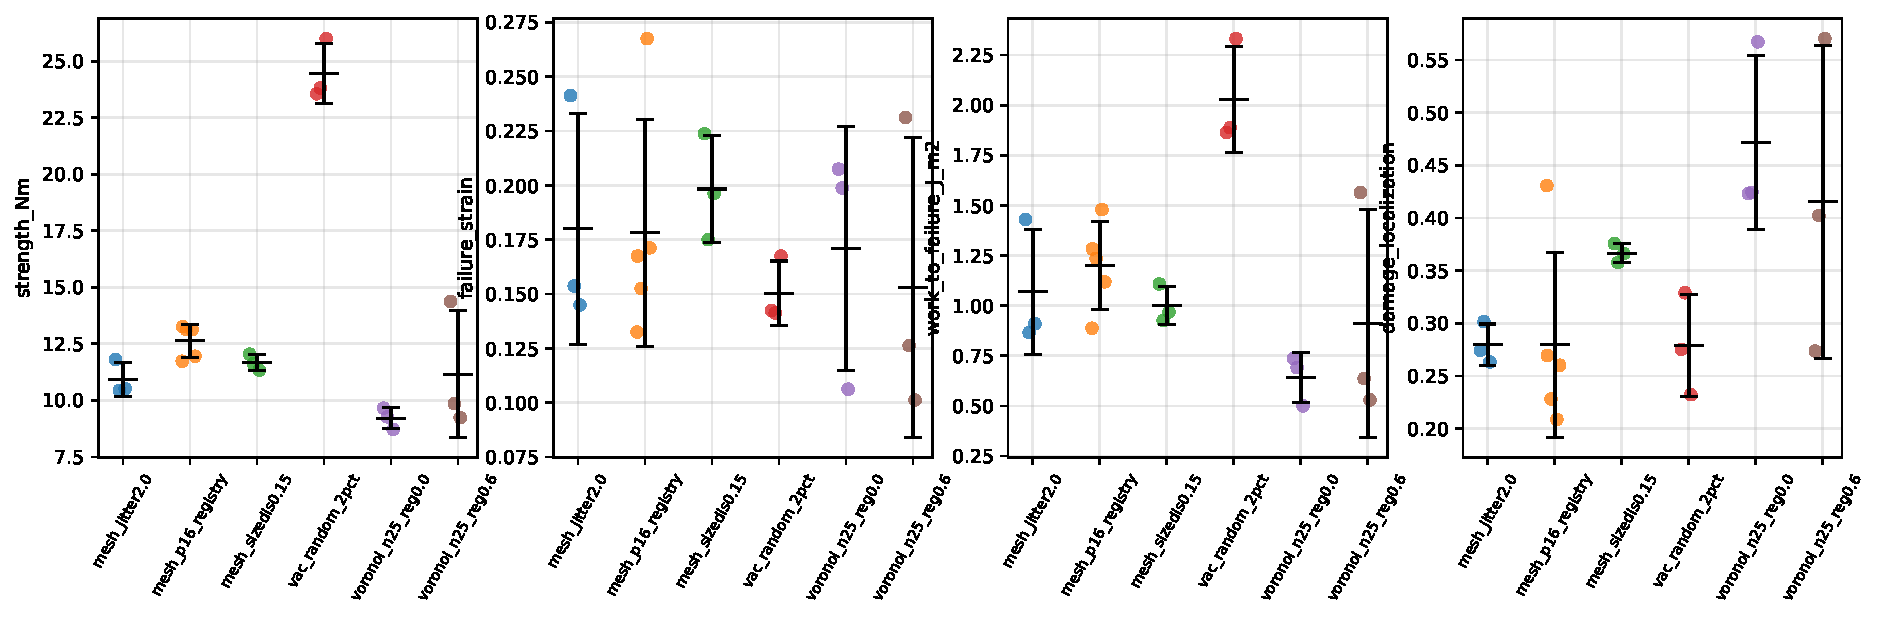
\includegraphics[width=1.0\textwidth]{campaign/seed_statistics.pdf}\caption{Random-seed statistics (Stage 6): individual simulations (dots) and mean +- standard deviation (black) of strength, failure strain, work to failure and damage localisation for stochastic architectures replicated with independent seeds.}\label{fig:seeds}\end{figure}
\subsection{Localised versus progressive fracture}
Three fracture modes were assigned automatically (Sec.~\ref{sec:damage}): single-avalanche brittle failure (26 of 85 Stage~1--6 designs), stepwise failure with a few discrete events (15) and progressive failure with many events and load retention (43). The entropy-based localisation $L$ separates \emph{crack-like} from \emph{distributed} damage but not abrupt from progressive: precracked and holed sheets have $L=0.44$--0.54 (the crack path occupies a few grid cells), whereas periodic meshes that fail in one avalanche spread that avalanche over all equivalent ligaments ($L\approx0.2$--0.35), so their damage is delocalised in space but not in strain (Fig.~\ref{fig:loc}). The temporal signature -- number of discrete damage steps and post-peak strain range -- is therefore the operative distinction: abrupt designs have $3.5$ damage steps on average and a post-peak strain range below one increment, progressive designs $11$ steps and 5--15\% of additional strain. Across the design space the mode is set by the load-transfer capacity after the first local failure (Stage~4): many parallel ligaments of moderate strength dispersion (fine meshes, jittered meshes, load-parallel-vein meshes, distributed vacancies) fail sequentially; few wide strips, clustered defects and single flaws fail in one event. Random networks combine a localised crack path with several steps (they fail thinnest-ligament first, then re-localise).

\begin{figure}[H]\centering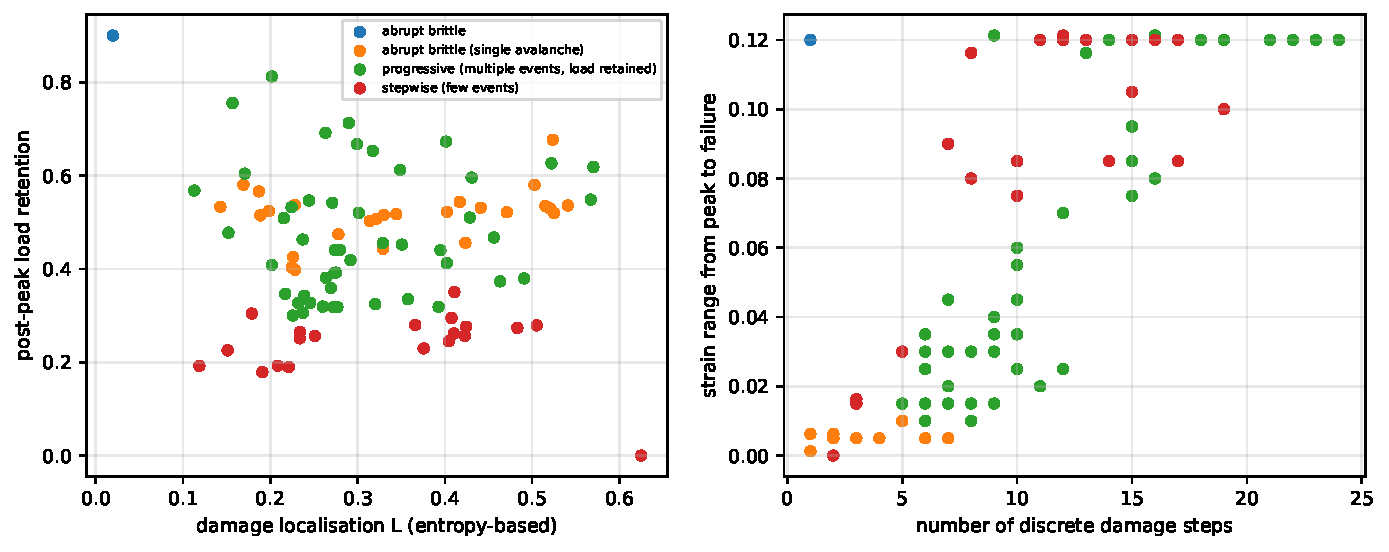
\includegraphics[width=1.0\textwidth]{campaign/localisation_modes.pdf}\caption{Localised versus progressive fracture: damage localisation, post-peak load retention, number of discrete damage events and post-peak strain range, coloured by the automatically assigned fracture-mode class.}\label{fig:loc}\end{figure}
\subsection{Pareto analysis}
No scalar objective was optimised; instead the non-dominated sets of six objective pairs were extracted from the full database (Fig.~\ref{fig:pareto}, all structures; the porous-only fronts are in \texttt{figures/\allowbreak campaign/\allowbreak pareto\_fronts\_porous.pdf}). The pristine sheets dominate every front that does not reward porosity, so the informative fronts are those restricted to porous designs. On the strength--failure-strain front the load-parallel slit designs (25.4--25.6\,N/m) occupy the strong end, the 45$^\circ$ slit lattice the ductile end (0.32 failure strain through geometric re-stiffening), and the low-porosity mesh in between; on strength--work only the two parallel-slit designs are non-dominated; on stiffness--failure strain the front adds the $0/90^\circ$ strut lattice and the hierarchy $\times$ anisotropy mesh (17.5\,N/m, 0.26 failure strain); on work--load retention the coarse meshes, the three-level mesh and the slits share the front; on specific work per atom versus porosity the sparse strut lattices ($\phi=0.45$) are non-dominated despite low strength. The fronts are structurally diverse (slits, coarse meshes, nested anisotropic meshes, strut lattices, a shear-like slit lattice) and no family dominates more than two objective pairs; the trade-off most relevant to design is strength versus progressivity: the strongest porous designs (straight equivalent strips) fail in one avalanche, and the only designs that combine a strength above 16\,N/m with progressive failure are those with many straight, load-parallel ligaments of moderate dispersion (load-parallel-vein mesh, hierarchy $\times$ anisotropy mesh, 32\,\AA{} round-pore mesh).

\begin{figure}[H]\centering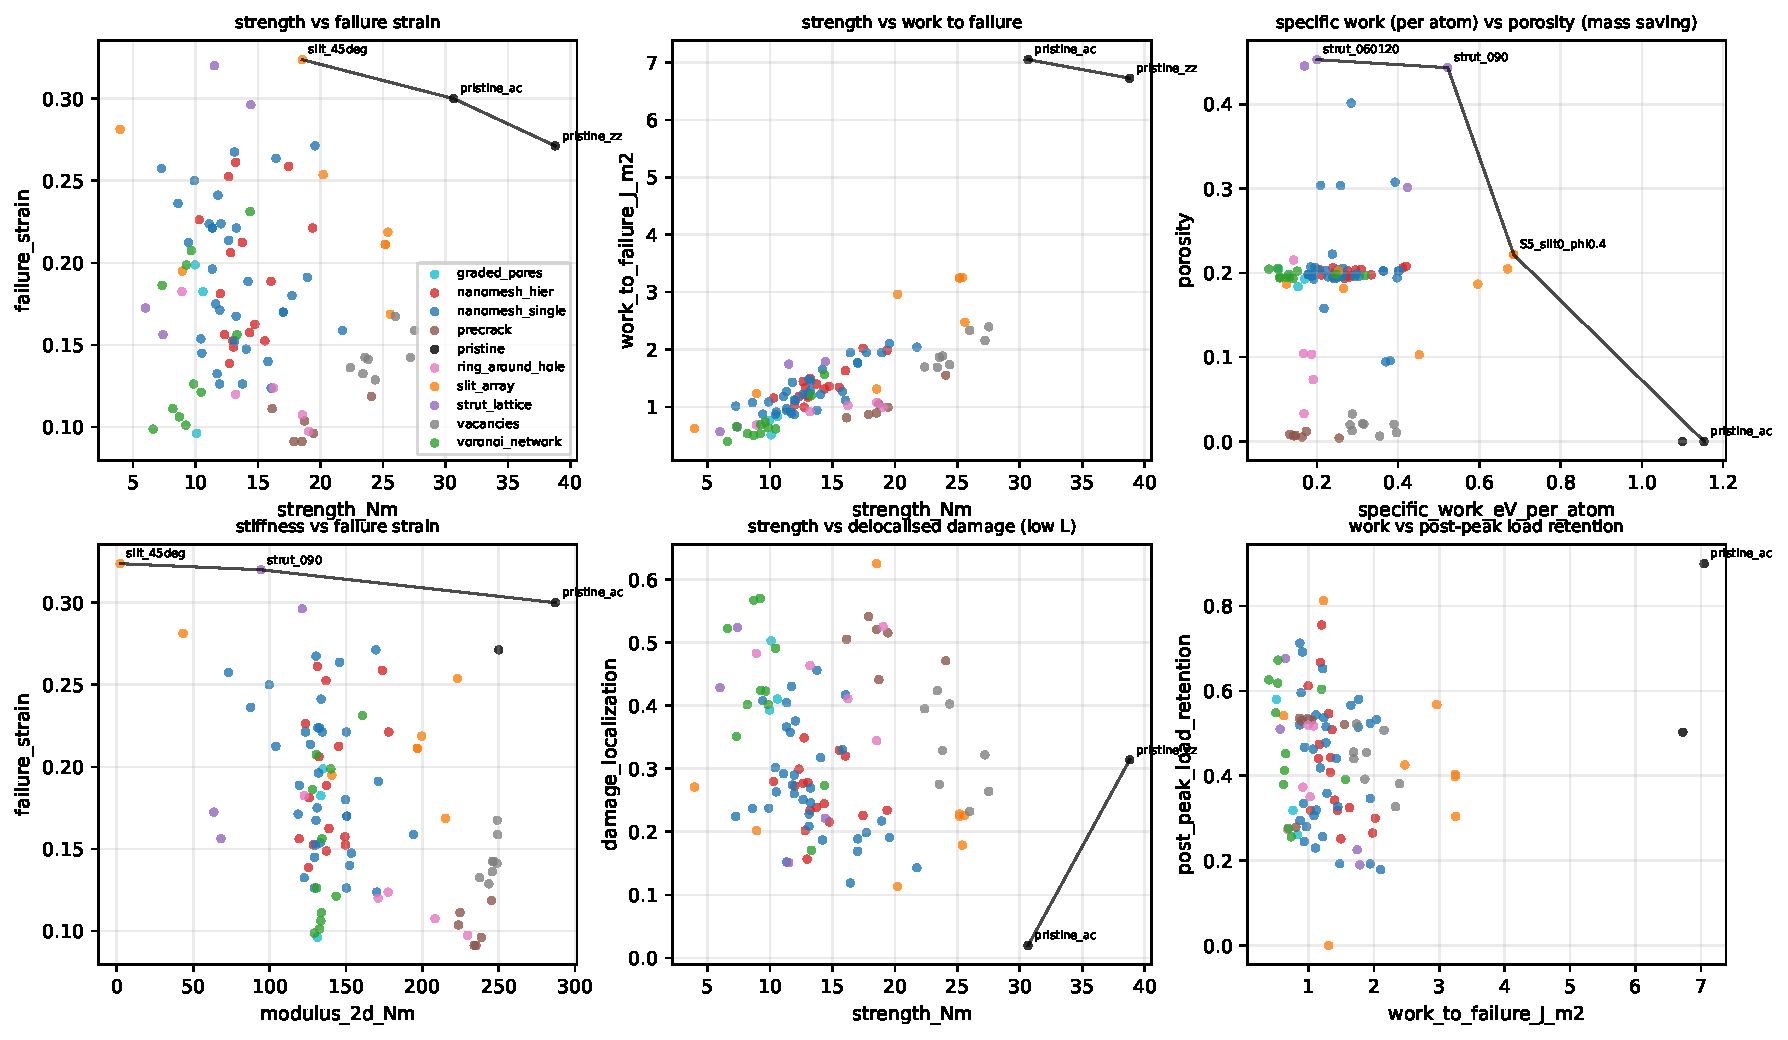
\includegraphics[width=1.0\textwidth]{campaign/pareto_fronts.pdf}\caption{Pareto analysis of all simulated structures: non-dominated sets (black lines, labelled) for six objective pairs; each point is one simulated architecture. The fronts are structurally diverse by construction of the design space (no optimiser was used to collapse onto one family).}\label{fig:pareto}\end{figure}
\subsection{Property charts and architecture atlas}
\label{sec:ashby}
Fig.~\ref{fig:ashby} condenses the campaign into Ashby-style property charts (log--log axes, one convex envelope per generator family, guidelines of constant specific property) and Fig.~\ref{fig:atlas} shows the relaxed structure of every simulated architecture next to its properties. Four readings follow directly from the charts.
\begin{itemize}
\item \textbf{Strength is not a rule of mixtures.} At a relative areal density of $\bar\rho = 0.8$ (63 structures within 0.77--0.83) the specific strength $\sigma/\bar\rho$ spans a factor of six, from 4.9\,N/m (slits perpendicular to the load) to 32.5\,N/m (slits parallel to the load), against 38.8\,N/m for the pristine zigzag sheet. Only the load-parallel slit arrays keep more than 80\% of the pristine specific strength; nanomeshes, hierarchical meshes and Voronoi networks at the same mass have medians of 16, 17 and 12\,N/m. The vertical spread at fixed density is the content of the campaign: net section, ligament width, alignment and lattice orientation, not mass, separate the families.
\item \textbf{Modulus is (almost) a rule of mixtures.} The specific modulus $Y/\bar\rho$ of every family with load-carrying ligaments lies between 110 and 275\,N/m (medians 150--250\,N/m against 245\,N/m for graphene), the strut lattices being lowest because their inclined ligaments bend. The single exception is the slit array at 45 degrees to the load, whose modulus collapses to 2.2\,N/m at the same density because its inclined ligaments rotate like a scissor before they stretch (Poisson ratio 0.96); the perpendicular array keeps 43\,N/m. The envelope of the slit family therefore spans two decades in modulus at one density.
\item \textbf{Work to failure grows with strength.} Across the porous structures $\log W$ scales with $\log\sigma_\mathrm{max}$ with a slope of 1.13 (correlation 0.84): the campaign found no architecture that buys energy absorption with strength. The upper right of the strength--work chart is occupied by the load-parallel slit arrays and the aligned hierarchical meshes, the lower left by Voronoi networks, graded meshes and flaw halos.
\item \textbf{Failure strain is not a family property.} Every major family spans failure strains from about 0.1 to 0.25--0.32, and the failure strain is uncorrelated with the strength (correlation of the logarithms 0.11 across the porous structures); it is set by the post-peak behaviour (load retention, ligament rotation) rather than by the peak.
\end{itemize}
All quantities are model results for the \rebo{} sheet under athermal quasi-static tension; the work to failure is the area under the stress--strain curve to loss of load-bearing capacity and is a proxy, not a fracture toughness.

\begin{figure}[H]\centering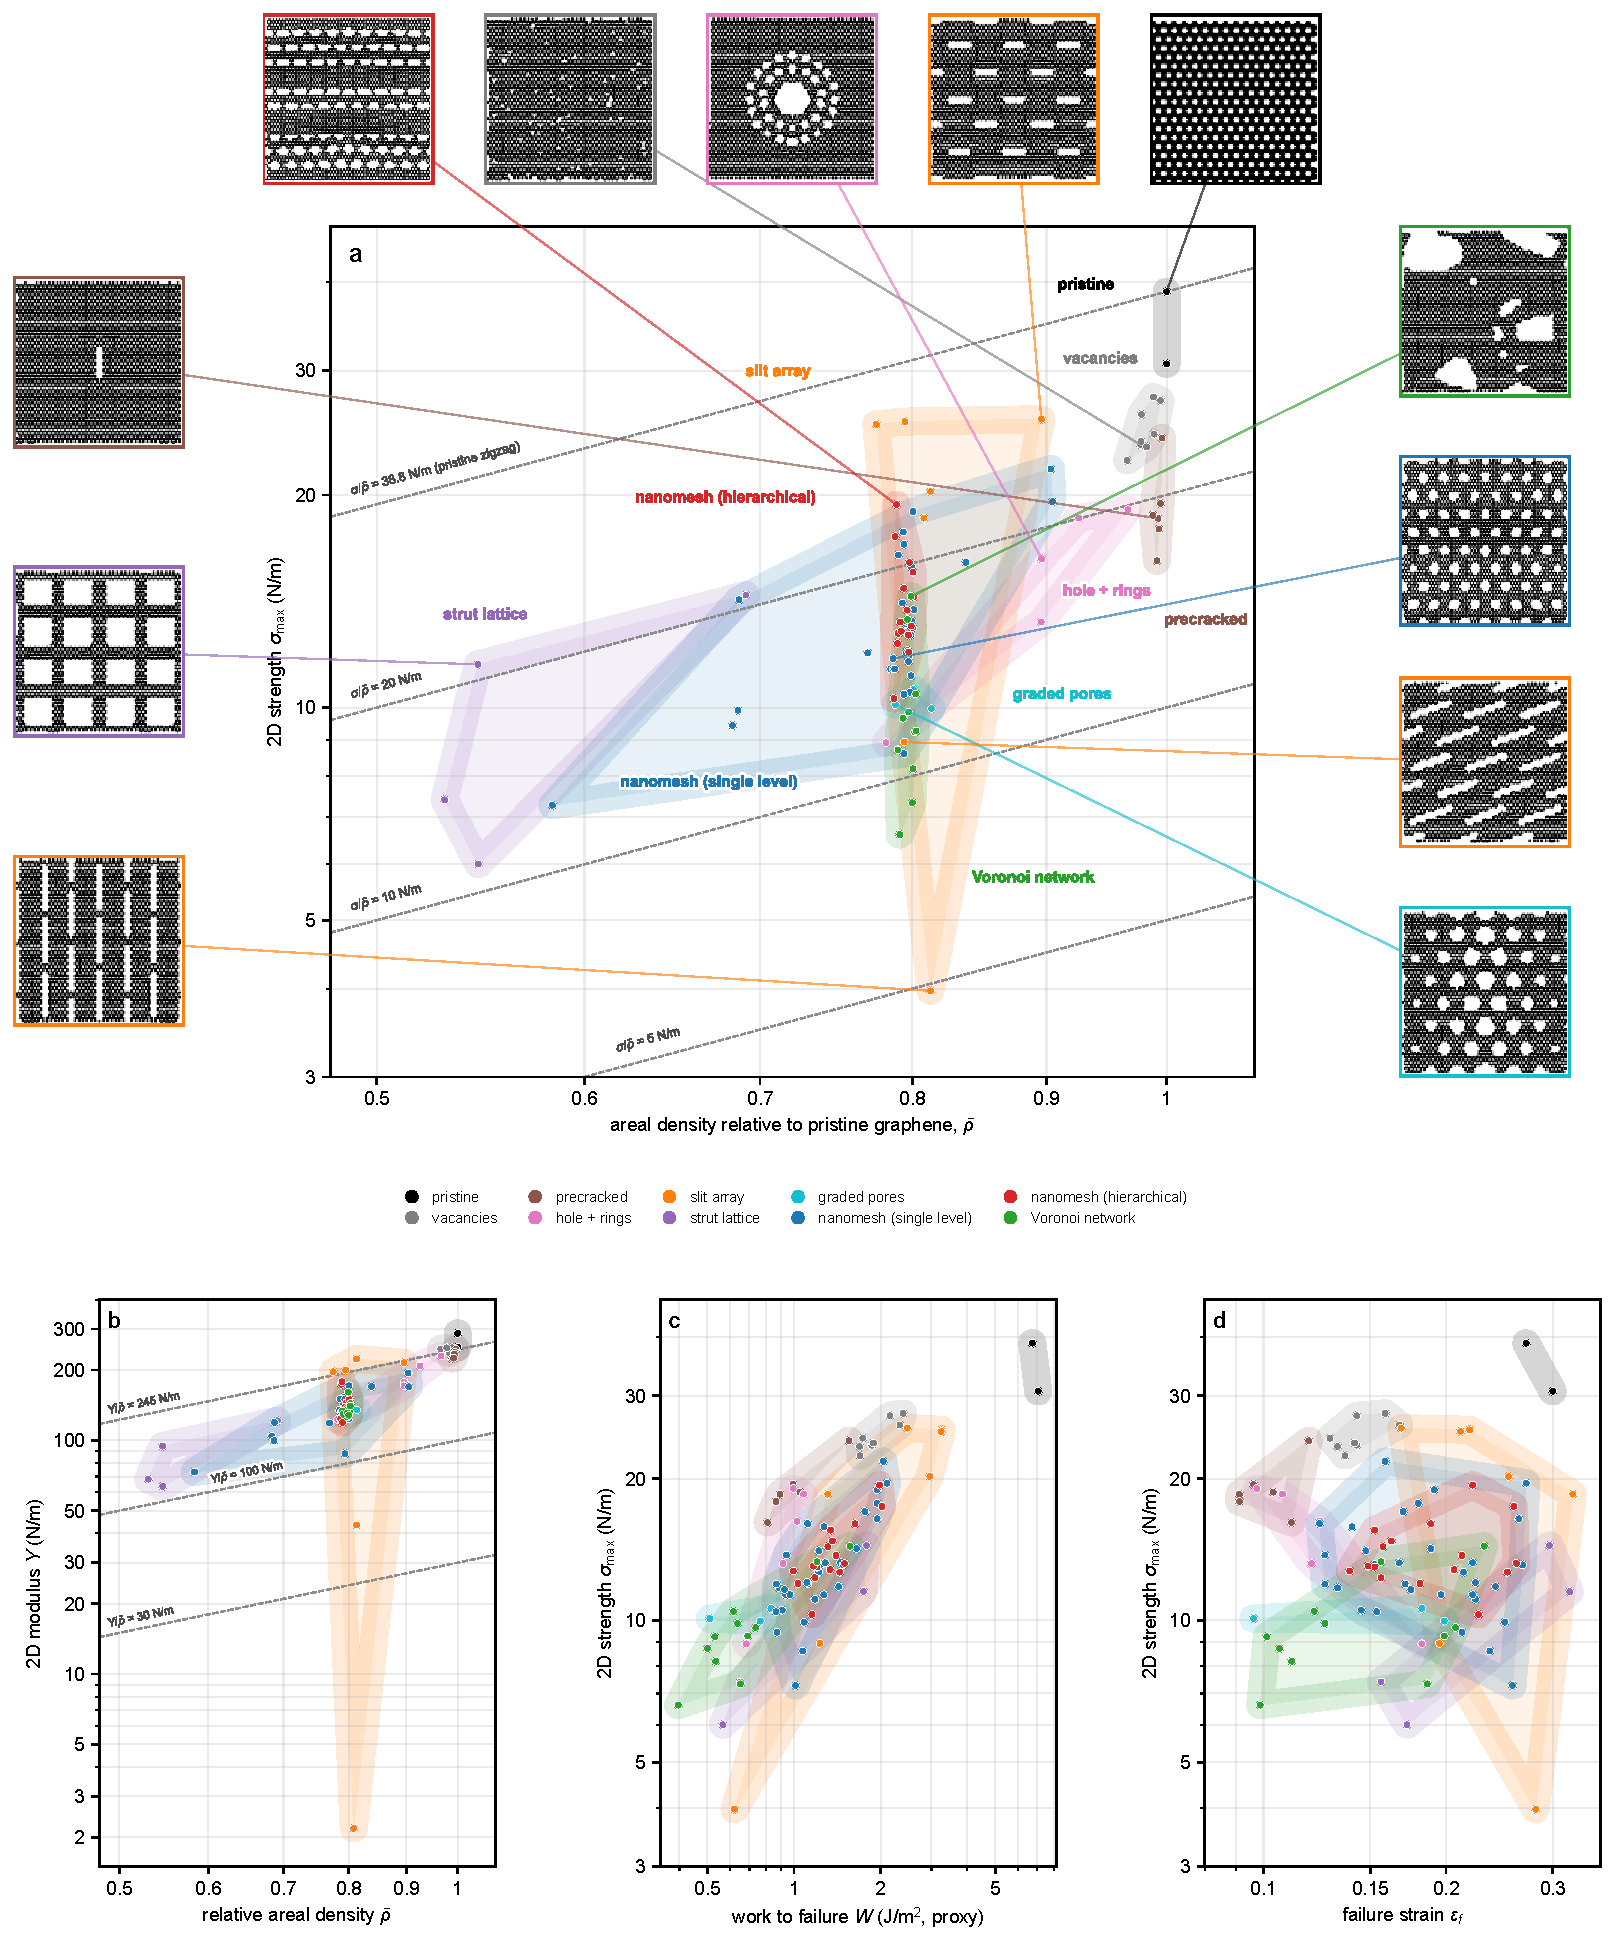
\includegraphics[width=0.98\textwidth]{campaign/ashby_overview.pdf}\caption{Ashby-style property charts of all 96 simulated architectures of the discovery campaign (model results: screened REBO2, athermal quasi-static uniaxial tension; 2D quantities). (a) 2D strength versus areal density relative to pristine graphene (log-log). Shaded envelopes are the convex hulls of each generator family, dashed guidelines are lines of constant specific strength sigma/rho (the top line is the pristine zigzag sheet), and the thumbnails show the relaxed structures of twelve representative designs (frame colour = family; leader lines point to their data points). (b) 2D modulus versus relative areal density with guidelines of constant specific modulus. (c) 2D strength versus work to failure (area under the stress-strain curve to loss of load-bearing capacity; a proxy, not a fracture toughness). (d) 2D strength versus failure strain. Every point is one simulation; Stage 6 seed replicates are included.}\label{fig:ashby}\end{figure}
\begin{figure}[H]\centering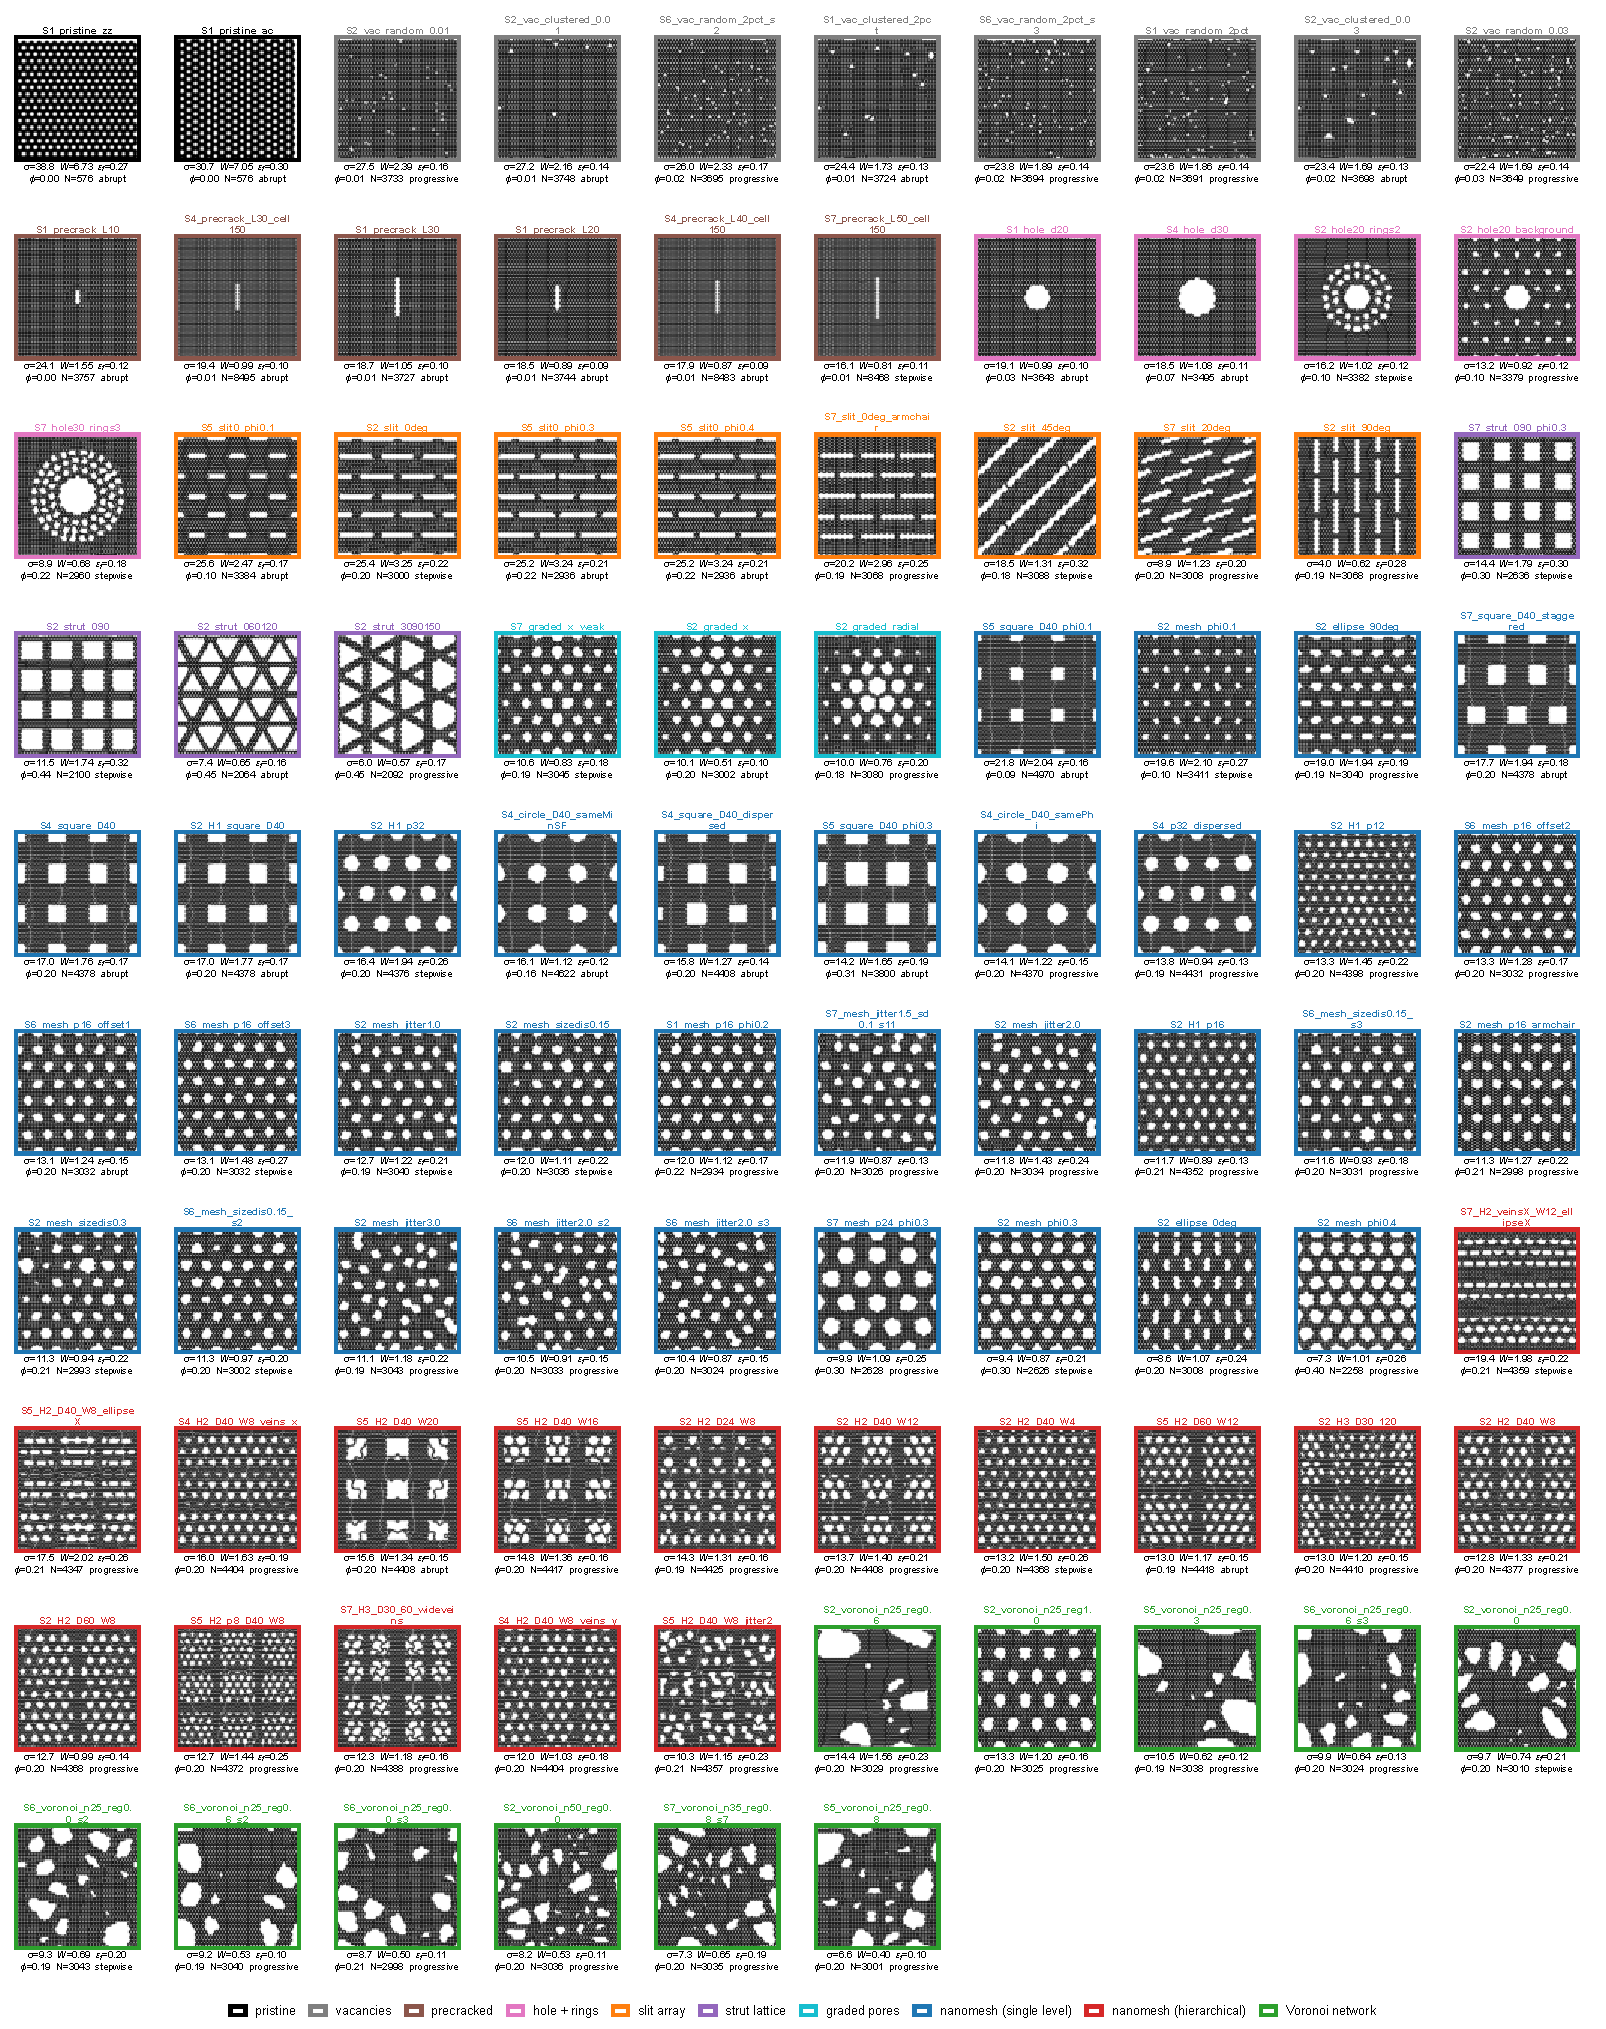
\includegraphics[width=0.98\textwidth]{campaign/architecture_atlas.pdf}\caption{Atlas of all 96 simulated architectures of the discovery campaign: relaxed structure of one periodic cell (atoms as black dots), grouped by generator family (frame colour, legend at the bottom) and ordered by decreasing 2D strength within each family. Below each structure: 2D strength sigma (N/m), work to failure W (J/m$^2$, proxy), failure strain, porosity phi, number of atoms N and fracture-mode class (abrupt = single avalanche, stepwise = few events, progressive = multiple events with load retained). Model results (screened REBO2, athermal quasi-static tension).}\label{fig:atlas}\end{figure}
\subsection{Stages 7--8: holdout predictions and evaluation}
\label{sec:holdout}
Twelve designs outside the training set were specified at the end of Stage 6. Their strength, modulus, failure strain, work to failure, damage localisation and fracture-mode class were predicted and written to a timestamped, hashed file before any of them was simulated (file written 2026-09-05 21:20:34, SHA-256 in Table~\ref{tab:holdout}; earliest holdout record 2026-09-05 21:52:25). The predictor is a documented, deliberately simple data-driven rule: a nearest-neighbour regression in descriptor space (porosity, minimum load-bearing solid fraction, ligament width, anisotropy, hierarchy level, disorder) over the Stage 1--6 records, with the net-section strength assigned by ligament class (Sec.~\ref{sec:mech}). Its failures therefore point at missing physics rather than at fitting noise. Table~\ref{tab:holdout} and Fig.~\ref{fig:holdout} compare predictions with observations.

Where the net-section rule applies unchanged, the predictions are accurate: the 90-degree strut lattice at 30\% porosity (14.4 predicted, 14.4 observed), the 50\,\AA{} crack in a 150\,\AA{} cell (16.3 vs 16.1\,N/m, confirming the lattice-trapping plateau at a crack length and cell size not used before), the three-level mesh with wide veins (11.7 vs 12.3), the jittered mesh with strength dispersion (12.3 vs 11.9), the 24\,\AA{} mesh at 30\% porosity (10.4 vs 9.9) and the staggered square mesh (19.3 vs 17.7\,N/m) all fall within 10\%. Over the twelve designs the median absolute error of the strength prediction is 14\% (Stage 4 discriminating experiments: 6.5\%), of the failure strain 17\%, of the work to failure 20\%, of the damage localisation 10\% and of the 2D modulus 11\%.

The five larger misses are the scientifically informative part of the test:
\begin{itemize}
\item \emph{Slit array rotated by 20 degrees} (predicted 23.9, observed 8.9\,N/m). The predictor treated a nearly load-parallel slit array like a parallel one. In the simulation the slit tips of neighbouring rows overlap along the load direction, and the ligaments between them fail by en-echelon crack coalescence (Fig.~\ref{fig:comparison_slit_orientation_echelon}), a mechanism that did not occur anywhere in the training set. The strength lies far below both the parallel (25.4\,N/m) and the 45-degree (18.5\,N/m) arrays of Stage 2 and closer to the perpendicular array (4.0\,N/m), although the sheet then fails progressively along the echelon paths and retains about 8\,N/m to 19\% strain. Load-path alignment is therefore not a monotonic function of angle; it is lost as soon as the tips of adjacent slit rows overlap along the load.
\item \emph{Load-parallel veins combined with load-elongated fine pores} (predicted 13.3, observed 19.4\,N/m; Fig.~\ref{fig:comparison_aligned_hierarchy_synergy}). This is the strongest nested design of the campaign; it failed in a few steps (19.4 to 11.8\,N/m at the first event) and its work to failure (2.0\,J/m$^2$) equals that of the best Stage 5 nested design, which had square veins. The two orientation effects act on different length scales and their benefits add; the nearest-neighbour predictor averaged over nested designs with and without alignment and could not represent the combination.
\item \emph{Parallel slits in armchair-oriented graphene} (predicted 24.0, observed 20.2\,N/m). The predictor had no lattice-orientation input. The net-section rule with the armchair intrinsic strength of Stage 1 (30.7 instead of 38.8\,N/m) predicts $25.4 \times 30.7/38.8 = 20.1$\,N/m, within 1\% of the observation: the ligament strength inherits the chirality dependence of the pristine sheet.
\item \emph{Flaw halo of three rings around a 30\,\AA{} hole} (predicted 13.1, observed 8.9\,N/m) and \emph{graded mesh with a weak band} (15.4 vs 10.6\,N/m). Both were predicted from cell-averaged descriptors; both are controlled by their weakest cross-section. The rings turn the hole into a wider effective flaw bounded by thin, curved ligaments, and the graded sheet fails in its most porous band. Strength is a minimum, not an average, over cross-sections, as the Stage 5 gradient series had already indicated.
\item \emph{Voronoi network with 35 cells and regularity 0.8} (predicted 12.1, observed 7.3\,N/m). A new seed at a cell count outside the training range produced the weakest holdout. The miss is consistent with the seed-to-seed scatter of random networks measured in Stage 6 (9.2 to 14.4\,N/m for three seeds of the 25-cell network at regularity 0.6, Fig.~\ref{fig:seeds}) and with the disorder penalty of hypothesis H-D, not with a new mechanism.
\end{itemize}

The fracture-mode class was predicted correctly in 5 of 12 cases in the strict three-class sense (single avalanche; stepwise with few events; progressive with load retention) and in 10 of 12 cases in the binary sense (single avalanche versus multi-event). All five strict misses are confusions between the two multi-event classes. The two binary misses are the 50\,\AA{} crack, which advanced bond by bond before the instability so that lattice trapping made it stepwise rather than abrupt, and the armchair slit array, whose wide ligaments failed one after another (progressive rather than abrupt). Compared with Stage 4 (median strength error 6.5\%, mode accuracy 80\%) the holdouts were harder by design: they combined variables, extended ranges, and included one geometry, the rotated slit array, chosen to probe the limit of the alignment rule.

The holdout test changes the conclusions in four ways: (i) the net-section rule holds as a minimum over cross-sections with a chirality-dependent ligament strength; (ii) alignment benefits at different scales add, which makes the aligned two-level mesh the best nested architecture found; (iii) the alignment rule has a sharp angular limit set by tip overlap (en-echelon coalescence); (iv) data-driven interpolation over descriptors, even with the campaign's mechanistic classes built in, fails exactly where a mechanism changes, which is the argument for keeping the validated simulation in the loop rather than replacing it by a surrogate.

\begingroup\footnotesize\setlength{\tabcolsep}{4pt}
\begin{longtable}{>{\raggedright\arraybackslash}p{3.6cm}rrrrrrp{3.2cm}}
\caption{Holdout designs: predictions recorded before simulation (file hash in text) versus observations. Strength in N/m, work in J/m$^2$; ``mode'' = predicted/observed fracture-mode class (abrupt = single avalanche; stepwise = few events; progressive = multiple events with load retained).}\label{tab:holdout}\\
\toprule design & $\sigma_\mathrm{pred}$ & $\sigma_\mathrm{obs}$ & $\varepsilon^f_\mathrm{pred}$ & $\varepsilon^f_\mathrm{obs}$ & $W_\mathrm{pred}$ & $W_\mathrm{obs}$ & mode pred/obs\\ \midrule\endfirsthead
\toprule design & $\sigma_\mathrm{pred}$ & $\sigma_\mathrm{obs}$ & $\varepsilon^f_\mathrm{pred}$ & $\varepsilon^f_\mathrm{obs}$ & $W_\mathrm{pred}$ & $W_\mathrm{obs}$ & mode pred/obs\\ \midrule\endhead
S7\_\allowbreak{}H2\_\allowbreak{}veinsX\_\allowbreak{}W12\_\allowbreak{}ellipseX & 13.30 & 19.38 & 0.234 & 0.221 & 1.50 & 1.98 & progressive/stepwise\\
S7\_\allowbreak{}slit\_\allowbreak{}20deg & 23.90 & 8.94 & 0.194 & 0.195 & 2.64 & 1.23 & stepwise/progressive\\
S7\_\allowbreak{}square\_\allowbreak{}D40\_\allowbreak{}staggered & 19.30 & 17.73 & 0.161 & 0.180 & 1.87 & 1.94 & abrupt/abrupt\\
S7\_\allowbreak{}voronoi\_\allowbreak{}n35\_\allowbreak{}reg0.8\_\allowbreak{}s7 & 12.10 & 7.33 & 0.174 & 0.186 & 0.87 & 0.65 & stepwise/progressive\\
S7\_\allowbreak{}H3\_\allowbreak{}D30\_\allowbreak{}60\_\allowbreak{}wideveins & 11.70 & 12.33 & 0.185 & 0.156 & 1.12 & 1.18 & progressive/progressive\\
S7\_\allowbreak{}hole30\_\allowbreak{}rings3 & 13.10 & 8.92 & 0.139 & 0.183 & 0.83 & 0.68 & stepwise/stepwise\\
S7\_\allowbreak{}mesh\_\allowbreak{}p24\_\allowbreak{}phi0.3 & 10.40 & 9.91 & 0.172 & 0.250 & 0.90 & 1.09 & stepwise/progressive\\
S7\_\allowbreak{}precrack\_\allowbreak{}L50\_\allowbreak{}cell150 & 16.30 & 16.14 & 0.105 & 0.111 & 0.96 & 0.81 & abrupt/stepwise\\
S7\_\allowbreak{}graded\_\allowbreak{}x\_\allowbreak{}weak & 15.40 & 10.61 & 0.145 & 0.183 & 1.00 & 0.83 & progressive/stepwise\\
S7\_\allowbreak{}slit\_\allowbreak{}0deg\_\allowbreak{}armchair & 24.00 & 20.22 & 0.215 & 0.254 & 3.08 & 2.96 & abrupt/progressive\\
S7\_\allowbreak{}strut\_\allowbreak{}090\_\allowbreak{}phi0.3 & 14.40 & 14.43 & 0.229 & 0.296 & 1.69 & 1.79 & stepwise/stepwise\\
S7\_\allowbreak{}mesh\_\allowbreak{}jitter1.5\_\allowbreak{}sd0.1\_\allowbreak{}s11 & 12.30 & 11.95 & 0.193 & 0.126 & 1.14 & 0.87 & progressive/progressive\\
\bottomrule\end{longtable}\endgroup
Prediction errors (median absolute relative error): 2D modulus: 11\% (n=12), strength: 14\% (n=12), failure strain: 17\% (n=12), work to failure: 20\% (n=12), damage localisation: 10\% (n=12); fracture-mode class accuracy 42\%.
 Prediction file \path{experiments/predictions/holdout_predictions.json} written 2026-09-05 21:20:34 (SHA-256 2eb2d80ae41ff32b\ldots), evaluated 2026-09-06 01:52:23.
\begin{figure}[H]\centering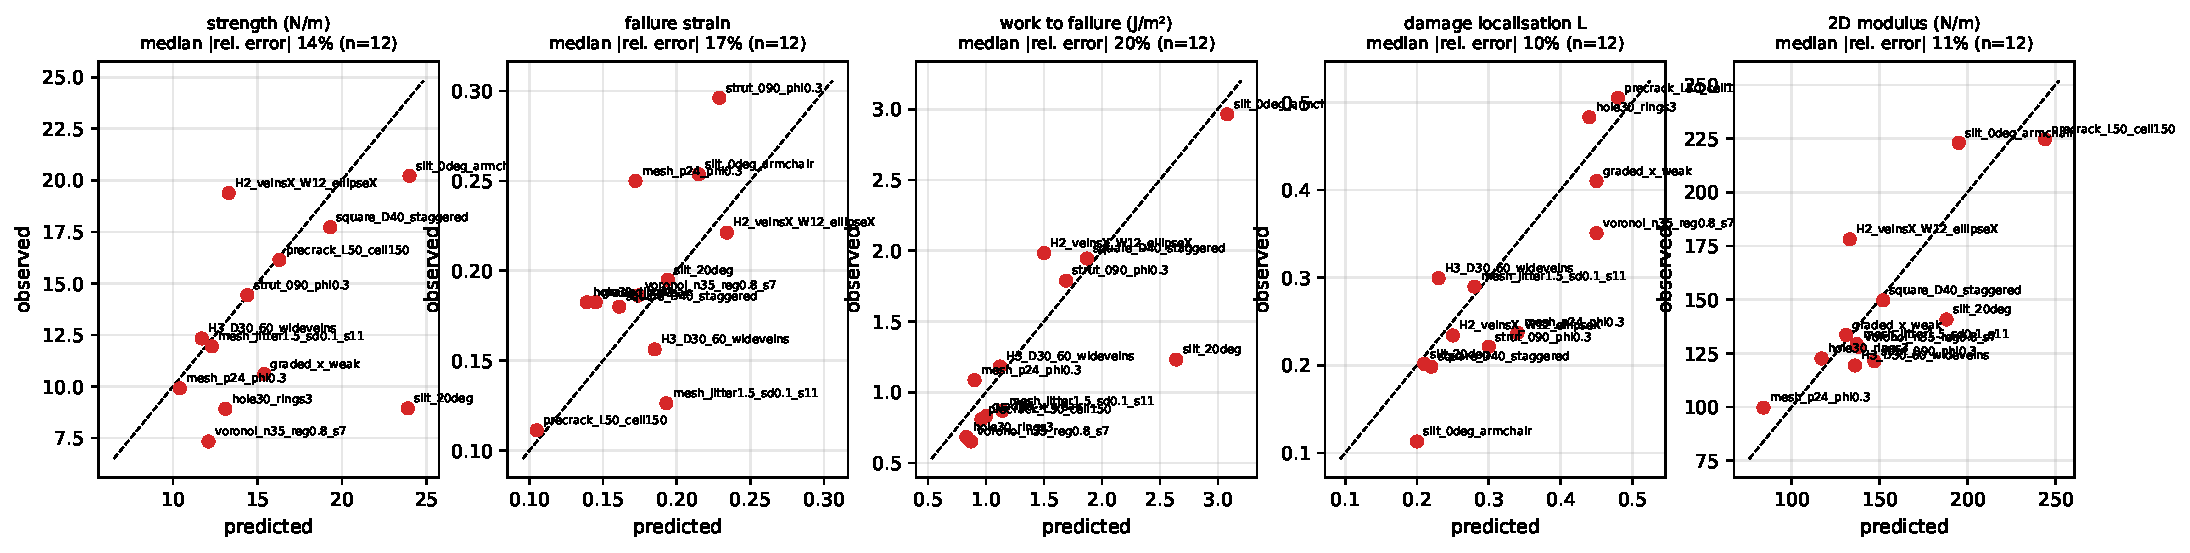
\includegraphics[width=0.9\textwidth]{campaign/holdout_prediction_vs_observation.pdf}\caption{Holdout evaluation (Stage 8): quantitative predictions recorded before the simulations (x) versus simulated values (y) for the unseen designs; dashed line = perfect prediction. Titles give the median absolute relative error.}\label{fig:holdout}\end{figure}
\subsection{Top-structure fracture progression}
\label{sec:top}
Ten structures were selected from the database for detailed fracture analysis, chosen for what they teach rather than for their strength alone: the two reference states (pristine zigzag graphene and the 20\,\AA{} precracked sheet), the strongest porous architecture, the most delocalised and the most localised failures, the key hierarchical design, the flaw-halo design, the weakest member of the matched-porosity hierarchy ladder, and the two holdout designs that changed the conclusions (the aligned two-level mesh and the 20-degree slit array). Two further categories, the largest work to failure (the 0.20-porosity parallel slit array, 3.25\,J/m$^2$, whose mechanism is that of the strongest design and which appears in Fig.~\ref{fig:comparison_slit_orientation_echelon}) and the load-parallel-vein mesh of Stage 4 (Fig.~\ref{fig:discriminating_experiments}), were analysed in the same way; their panels and movies are included in the archive but omitted here for length.

For each structure the progression panel shows event-selected frames rather than equally spaced ones: the relaxed state, the last frame before damage, the first bond loss, the peak load, the largest single propagation event, the first post-peak state and the final frame, each labelled with strain, 2D stress and the cumulative number of broken bonds. Atoms are coloured by their energy change relative to the relaxed state (the per-atom energies of the potential), and atoms that have lost a bond are circled. The before/after panels show the relaxed, peak-load and final configurations side by side. Movies of the same runs, with a synchronised stress--strain inset, are in \texttt{movies/} and in the ``Fracture progression'' panel of the app. The interpretation below each panel is a statement about the model; the ``interpretation'' of a structure as a mechanism was written after inspecting the frames and cross-checked against the matched comparisons of Stages 4 and 5.

\subsection{Reference: pristine zigzag graphene}
\begin{figure}[H]\centering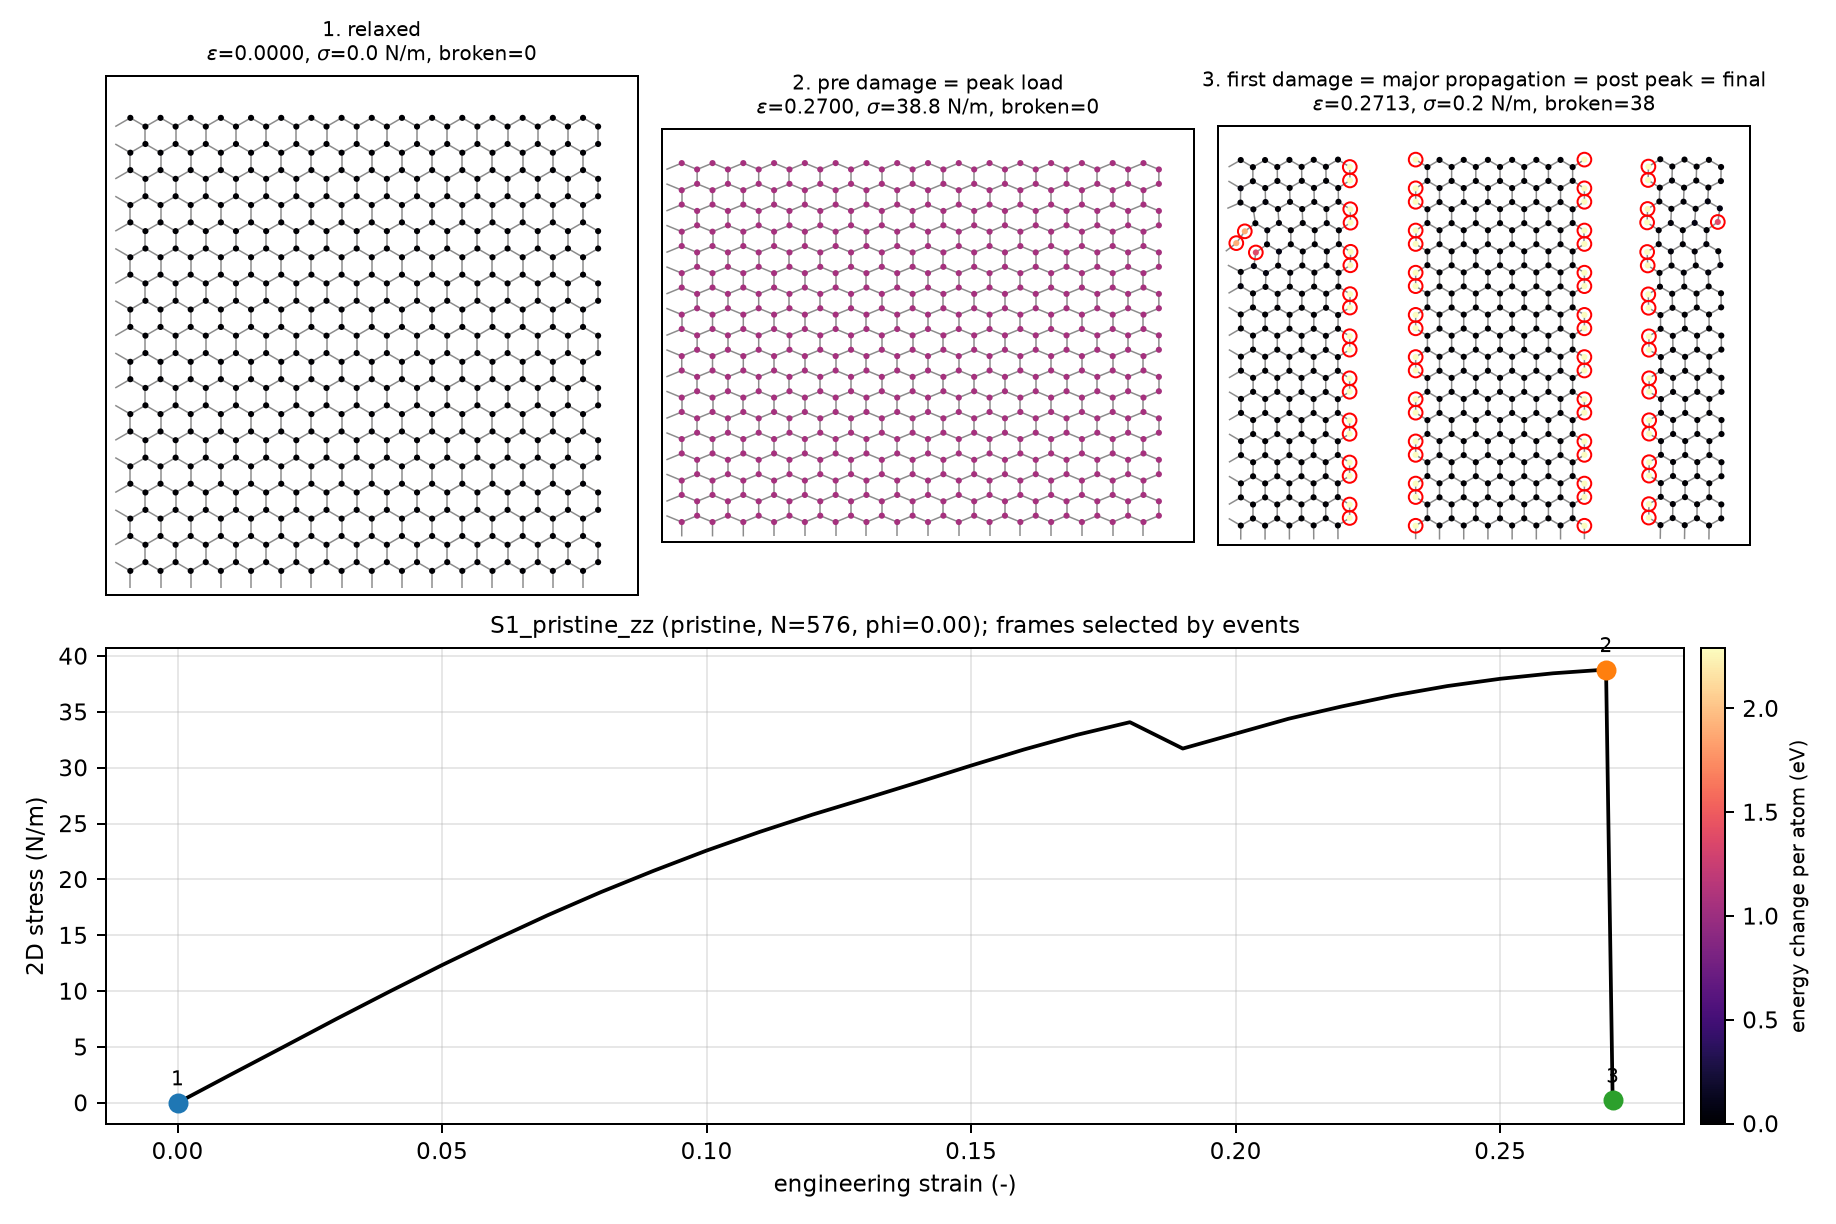
\includegraphics[width=\textwidth]{progression/progression_S1_pristine_zz_energy_rel.png}\caption{Fracture progression of S1\_pristine\_zz (pristine, N=576, porosity 0.00): event-selected frames (relaxed, pre-damage, first bond loss, peak load, major propagation, post-peak, final; colour = energy change per atom relative to the relaxed state, red circles = atoms that lost a bond) and the stress-strain curve with the displayed frames marked.}\label{fig:top0}\end{figure}
Reference state. The homogeneous zigzag sheet stores 6.7 J/m2 before a single instability at 27\% strain breaks every load-bearing bond row at once (36 bonds in one increment); the dip at 18\% is the transverse-branch switch of the model. Failure initiates nowhere in particular: all bonds along the load are equivalent, so there is no load path to redistribute to, and the fracture is maximally abrupt. Every porous design is weaker than this state, but many retain load after their peak, which the pristine sheet cannot.

\begin{figure}[H]\centering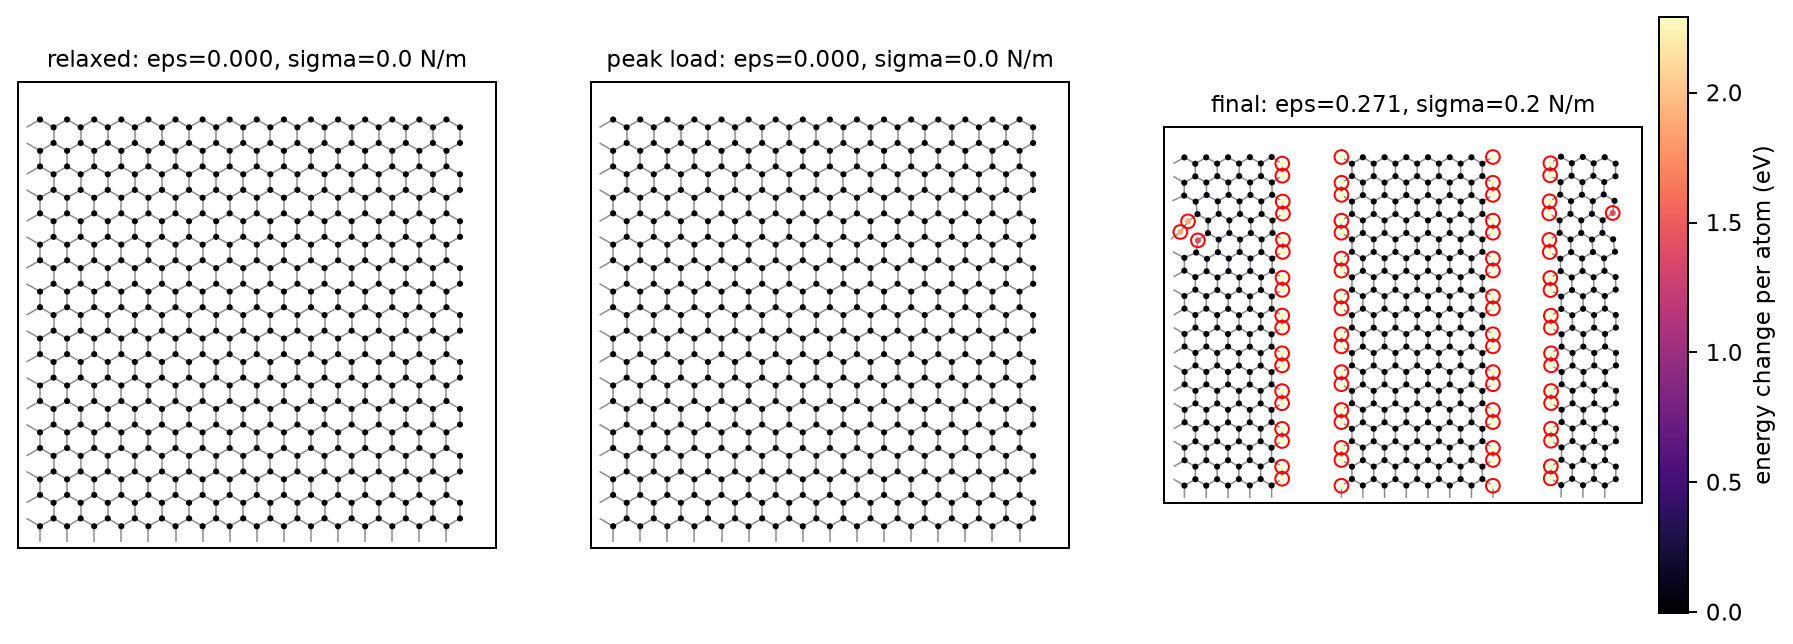
\includegraphics[width=0.95\textwidth]{progression/before_after_S1_pristine_zz.png}\caption{Before/after comparison for Reference: pristine zigzag graphene: relaxed, peak load and final configuration (colour: energy change per atom; red circles: atoms that lost a bond).}\end{figure}

\subsection{Reference: precracked graphene (20 A slit)}
\begin{figure}[H]\centering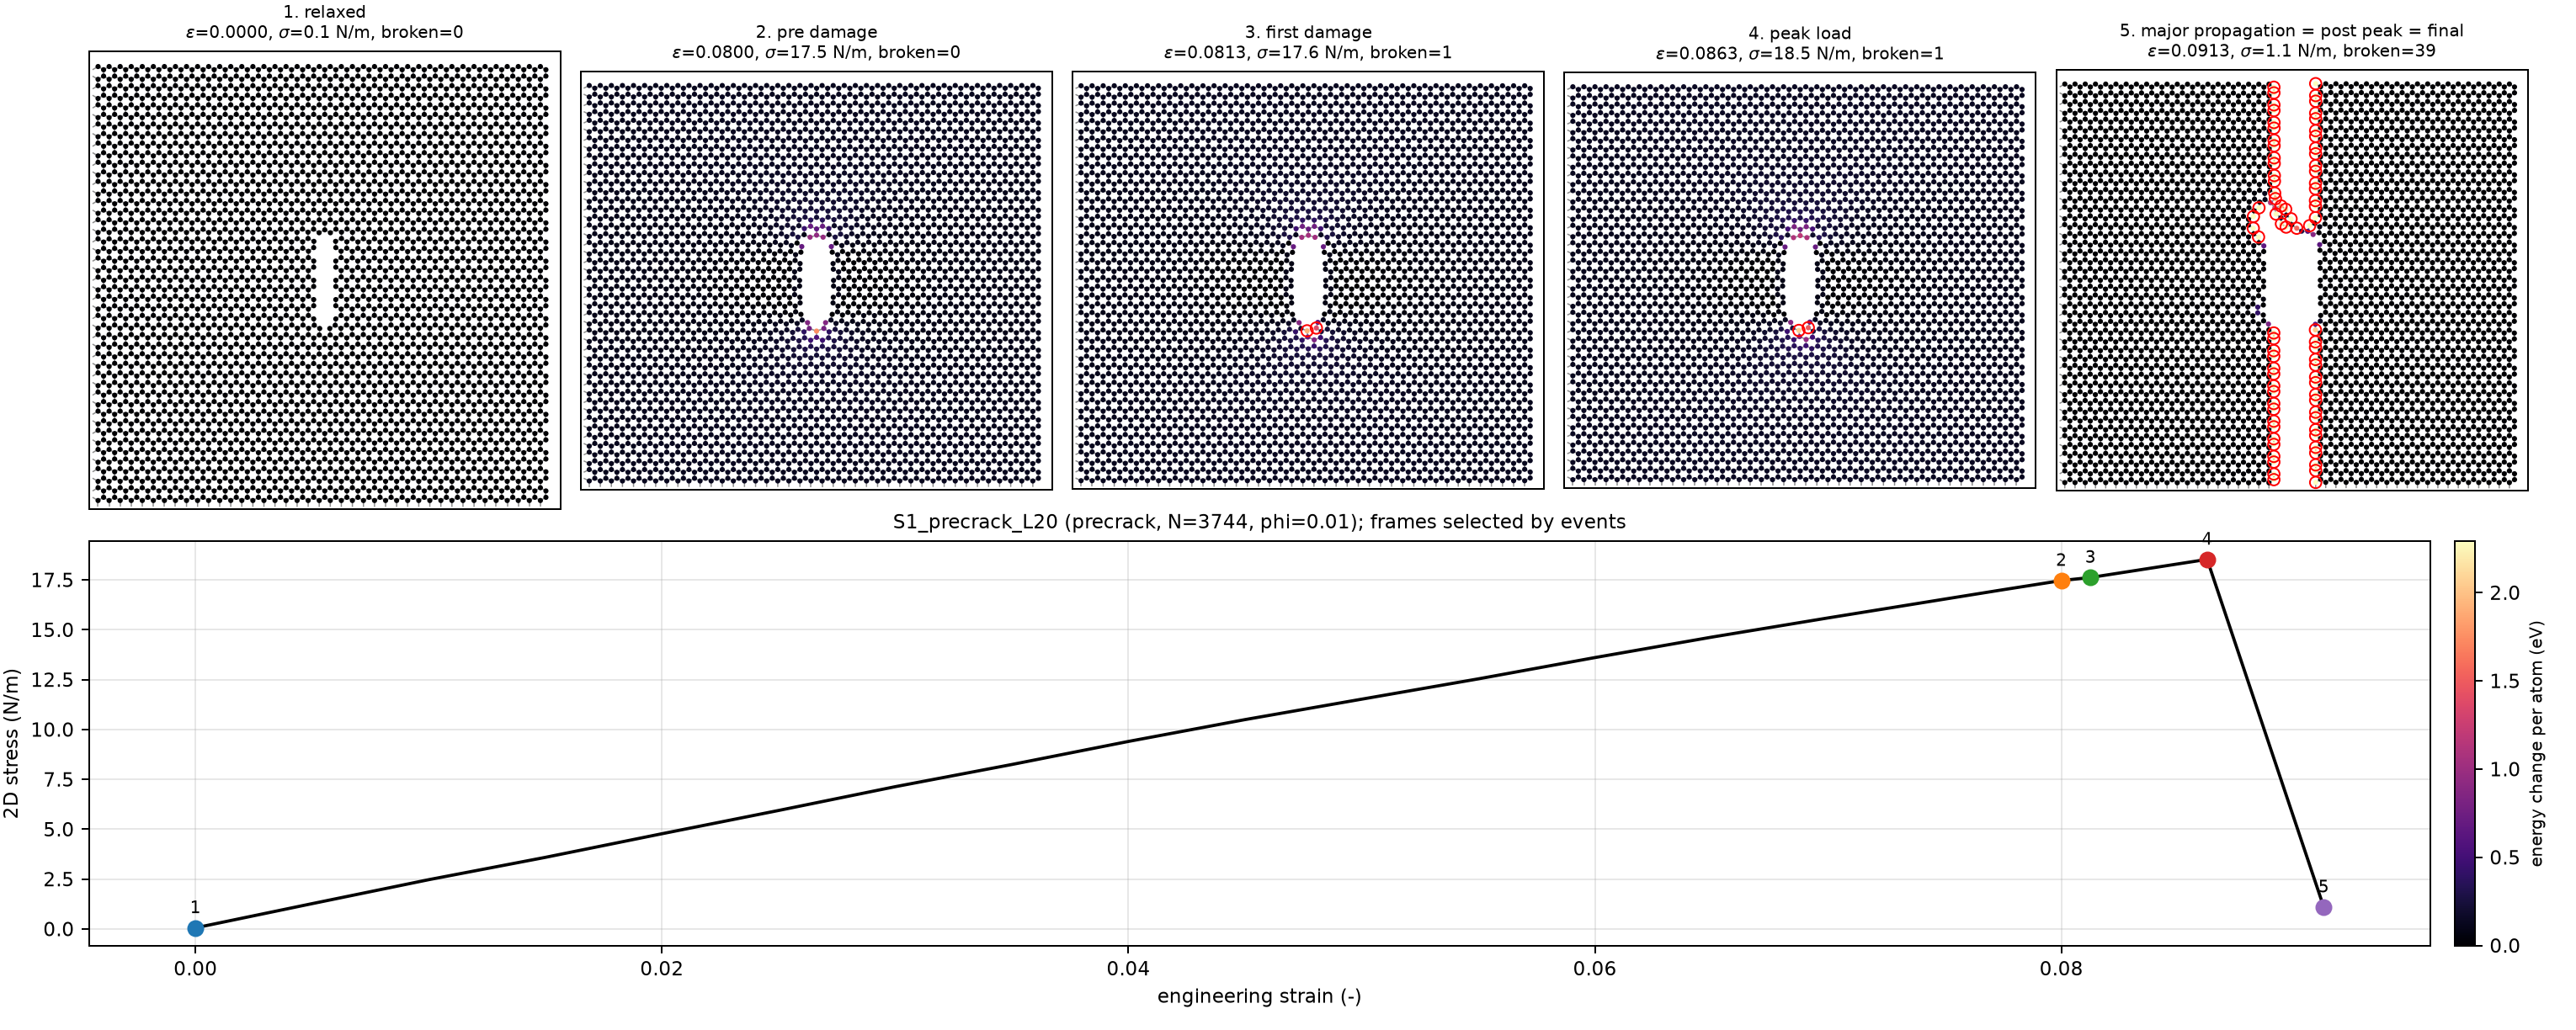
\includegraphics[width=\textwidth]{progression/progression_S1_precrack_L20_energy_rel.png}\caption{Fracture progression of S1\_precrack\_L20 (precrack, N=3744, porosity 0.01): event-selected frames (relaxed, pre-damage, first bond loss, peak load, major propagation, post-peak, final; colour = energy change per atom relative to the relaxed state, red circles = atoms that lost a bond) and the stress-strain curve with the displayed frames marked.}\label{fig:top1}\end{figure}
Flaw-sensitivity reference. Bonds first break at the two crack tips at 8.1\% strain, the crack then runs straight across the sheet perpendicular to the load in one avalanche at 8.6\% (18.5 N/m). Damage is confined to the crack plane (L = 0.52). Compared with the 10 A crack (24.1 N/m) the strength loss follows a Griffith-like trend, but the 30-50 A cracks do not weaken further: in this lattice the tip-bond configuration, not the crack length, sets the instability once the flaw exceeds ~20 A.

\begin{figure}[H]\centering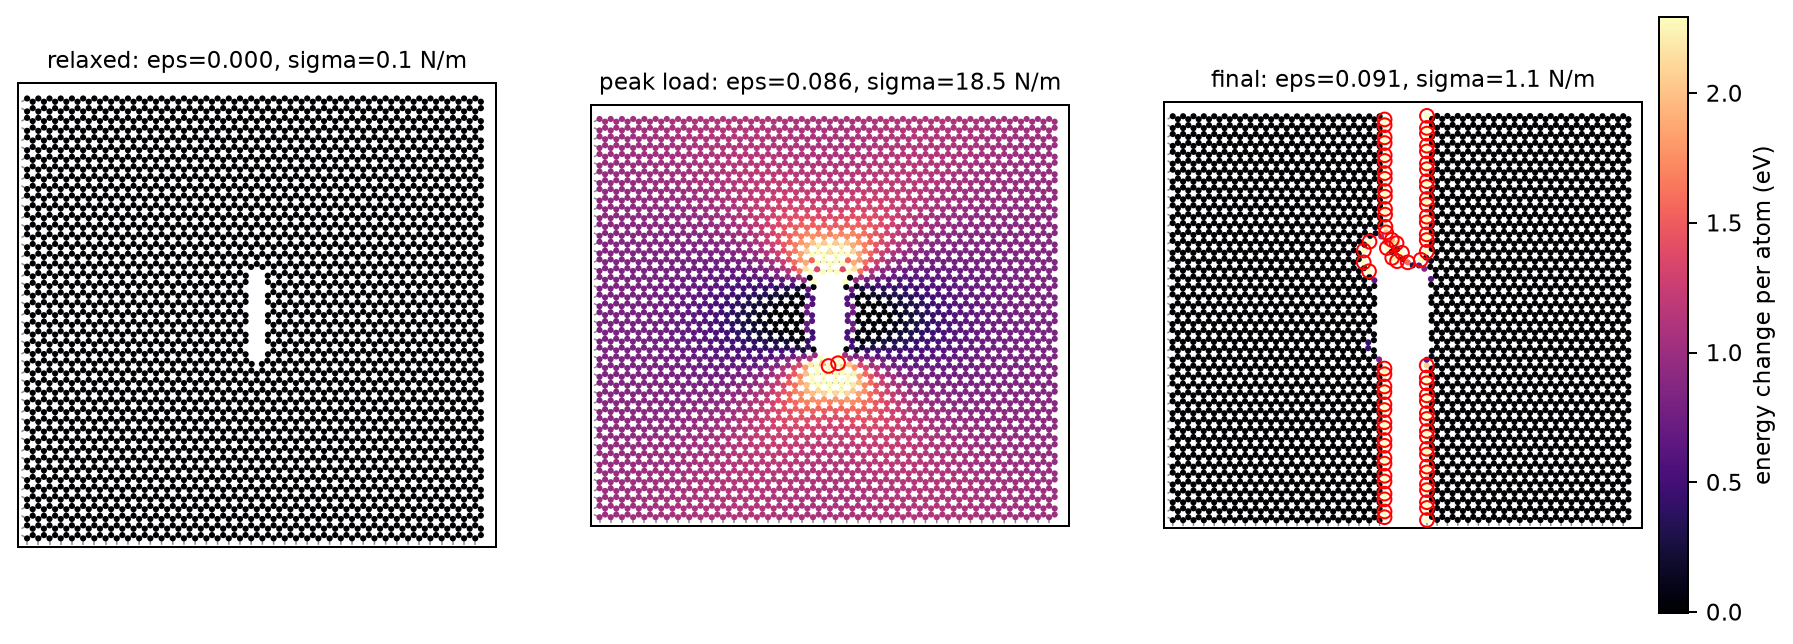
\includegraphics[width=0.95\textwidth]{progression/before_after_S1_precrack_L20.png}\caption{Before/after comparison for Reference: precracked graphene (20 A slit): relaxed, peak load and final configuration (colour: energy change per atom; red circles: atoms that lost a bond).}\end{figure}

\subsection{Strongest porous architecture}
\begin{figure}[H]\centering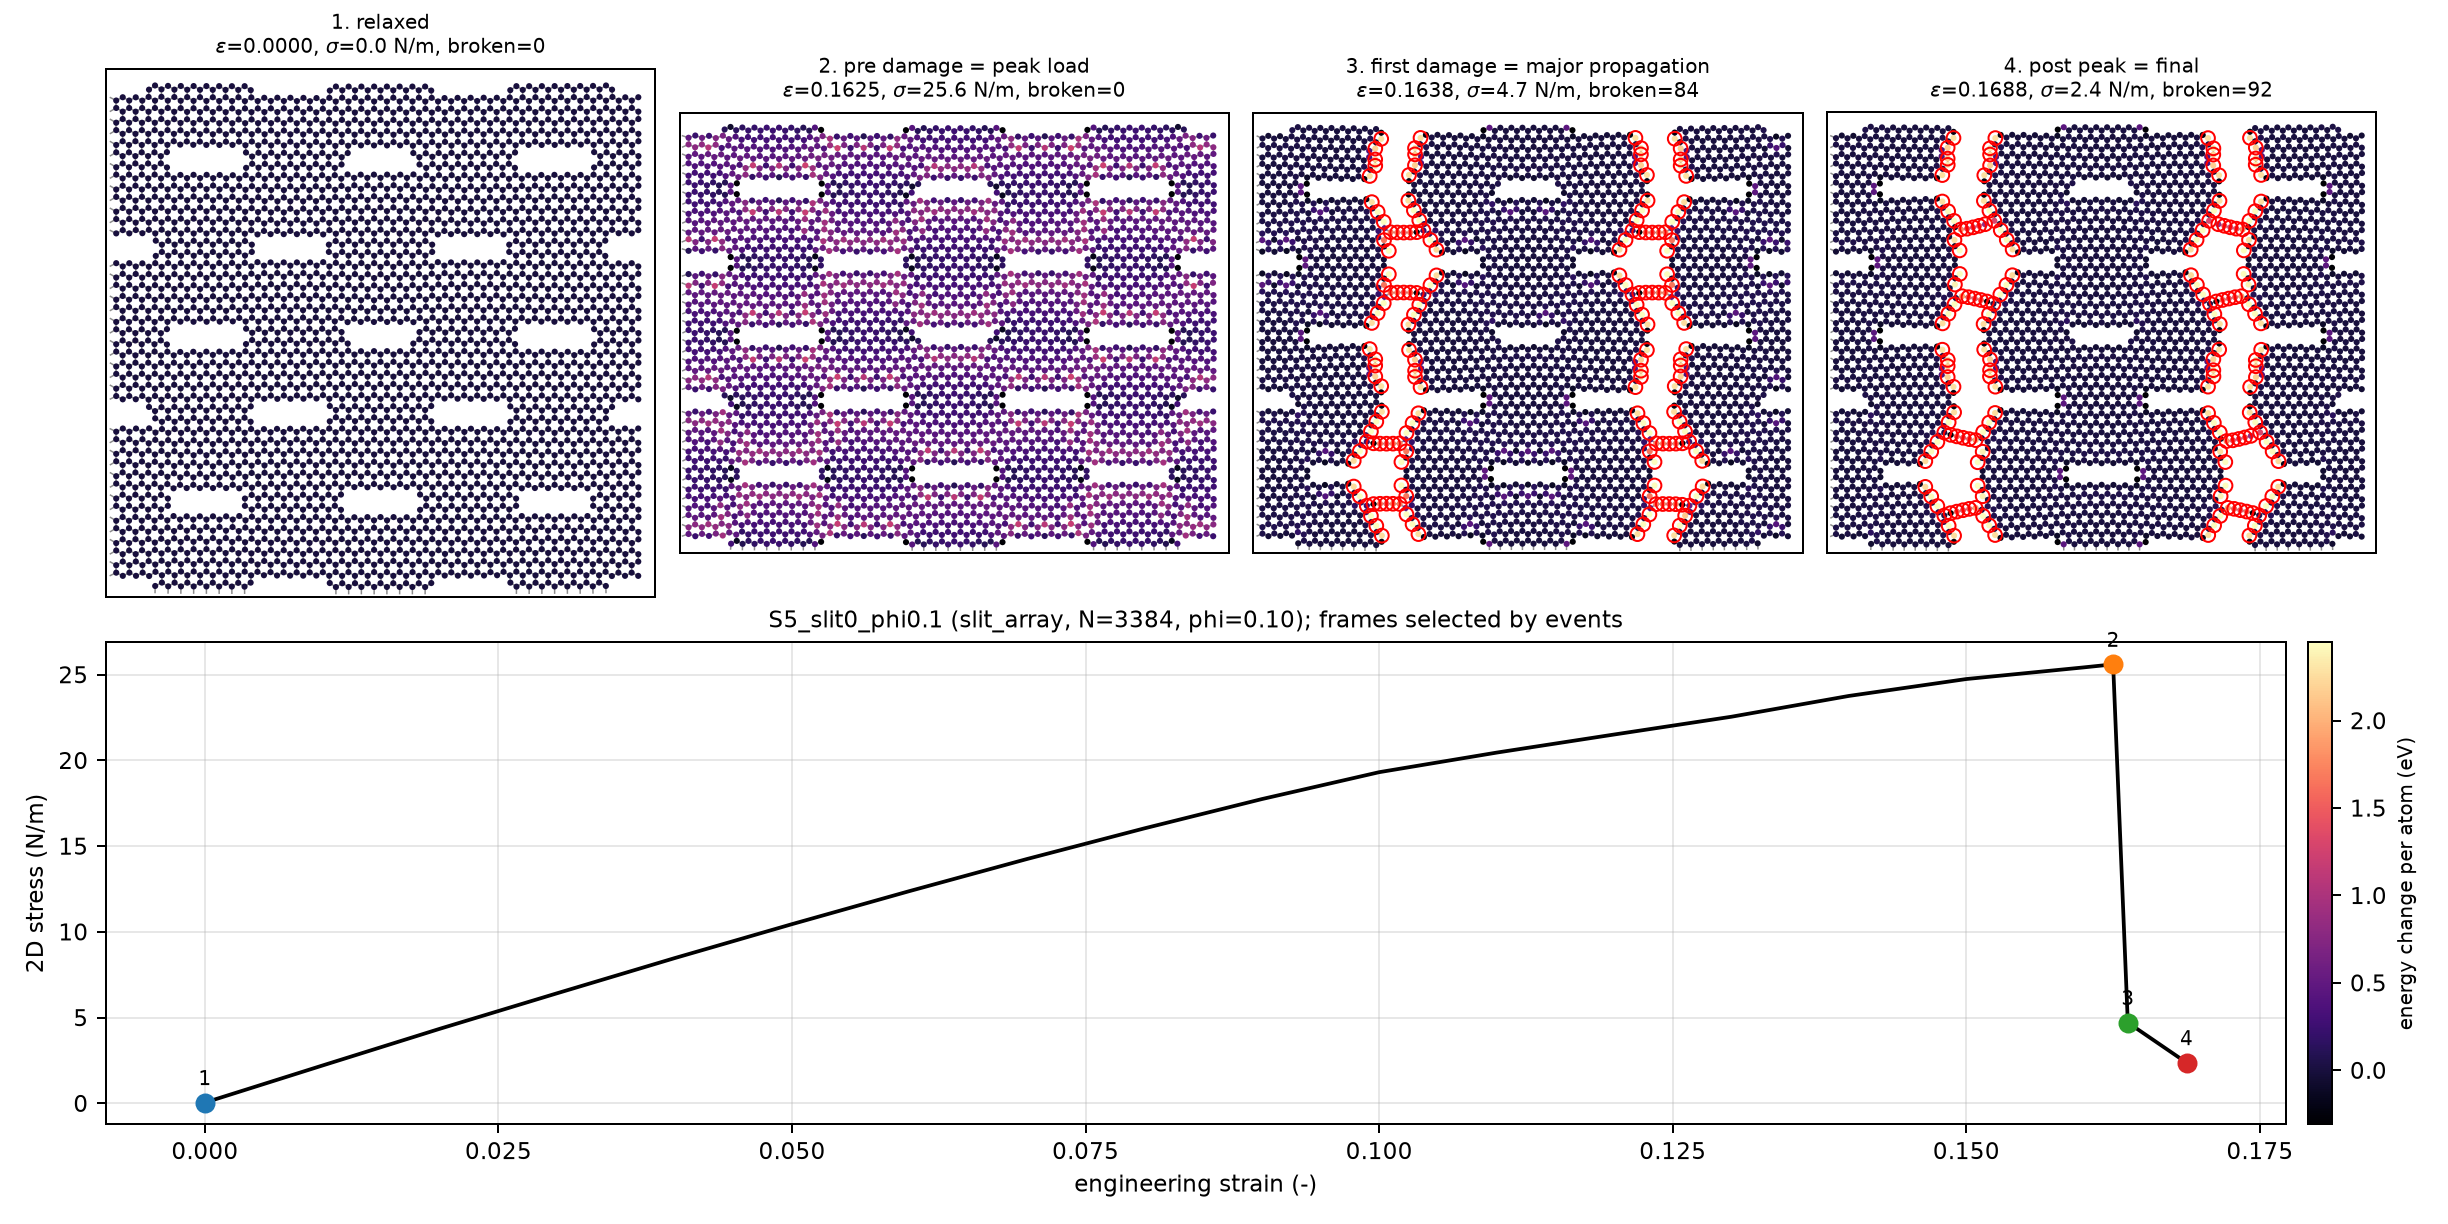
\includegraphics[width=\textwidth]{progression/progression_S5_slit0_phi0.1_energy_rel.png}\caption{Fracture progression of S5\_slit0\_phi0.1 (slit\_array, N=3384, porosity 0.10): event-selected frames (relaxed, pre-damage, first bond loss, peak load, major propagation, post-peak, final; colour = energy change per atom relative to the relaxed state, red circles = atoms that lost a bond) and the stress-strain curve with the displayed frames marked.}\label{fig:top2}\end{figure}
Strongest porous architecture (25.6 N/m at porosity 0.10) and identical in strength to its 0.20-porosity sibling: with slits parallel to the load the net section is set by the slit width only. The strips carry an almost uniform stress up to 20\% strain; failure starts at the bridges that connect neighbouring strips (the only places where the stress deviates from uniaxial) and all strips snap in the same increment. It is strong because its ligaments are straight and wide, and brittle for the same reason: all load paths are equivalent.

\begin{figure}[H]\centering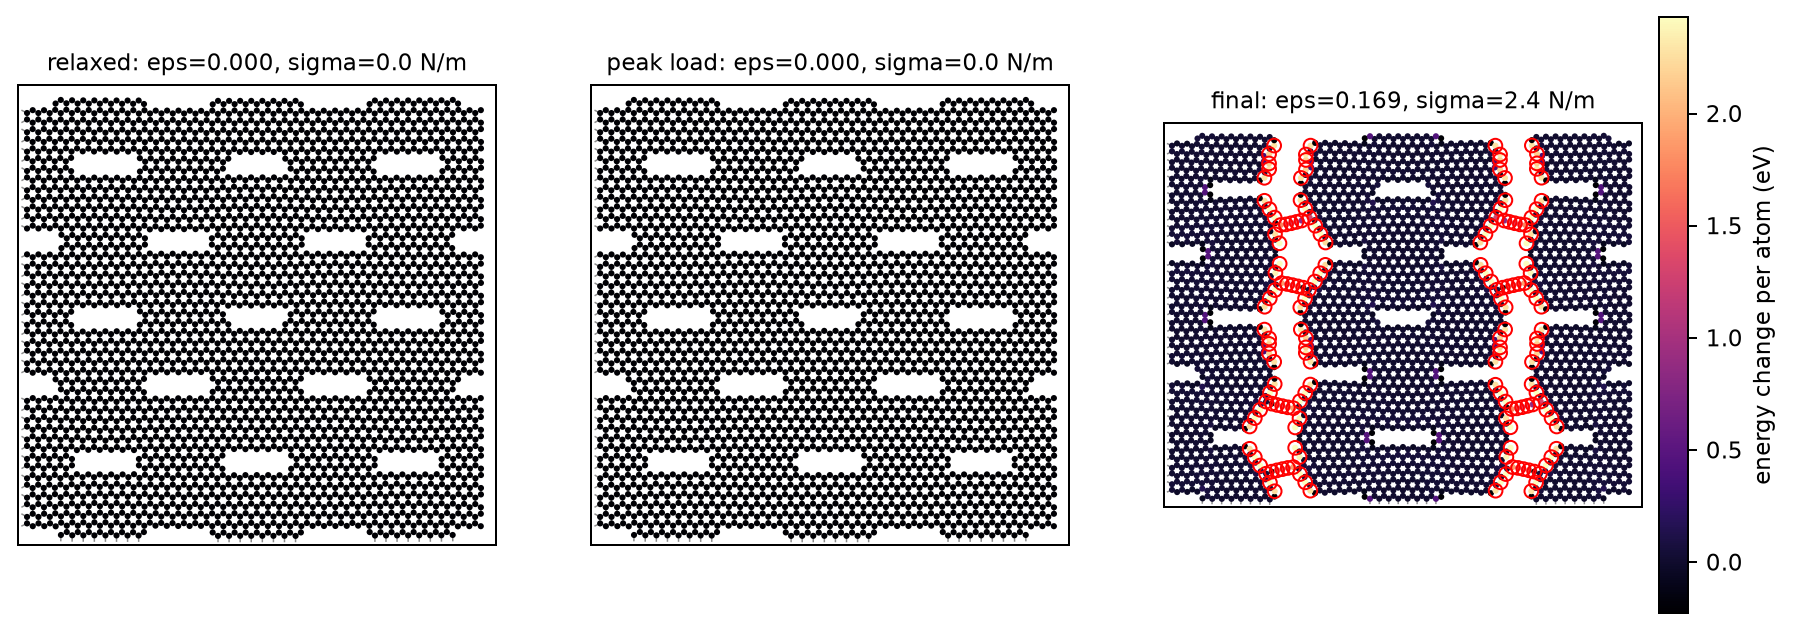
\includegraphics[width=0.95\textwidth]{progression/before_after_S5_slit0_phi0.1.png}\caption{Before/after comparison for Strongest porous architecture: relaxed, peak load and final configuration (colour: energy change per atom; red circles: atoms that lost a bond).}\end{figure}

\subsection{Most delocalised / progressive fracture}
\begin{figure}[H]\centering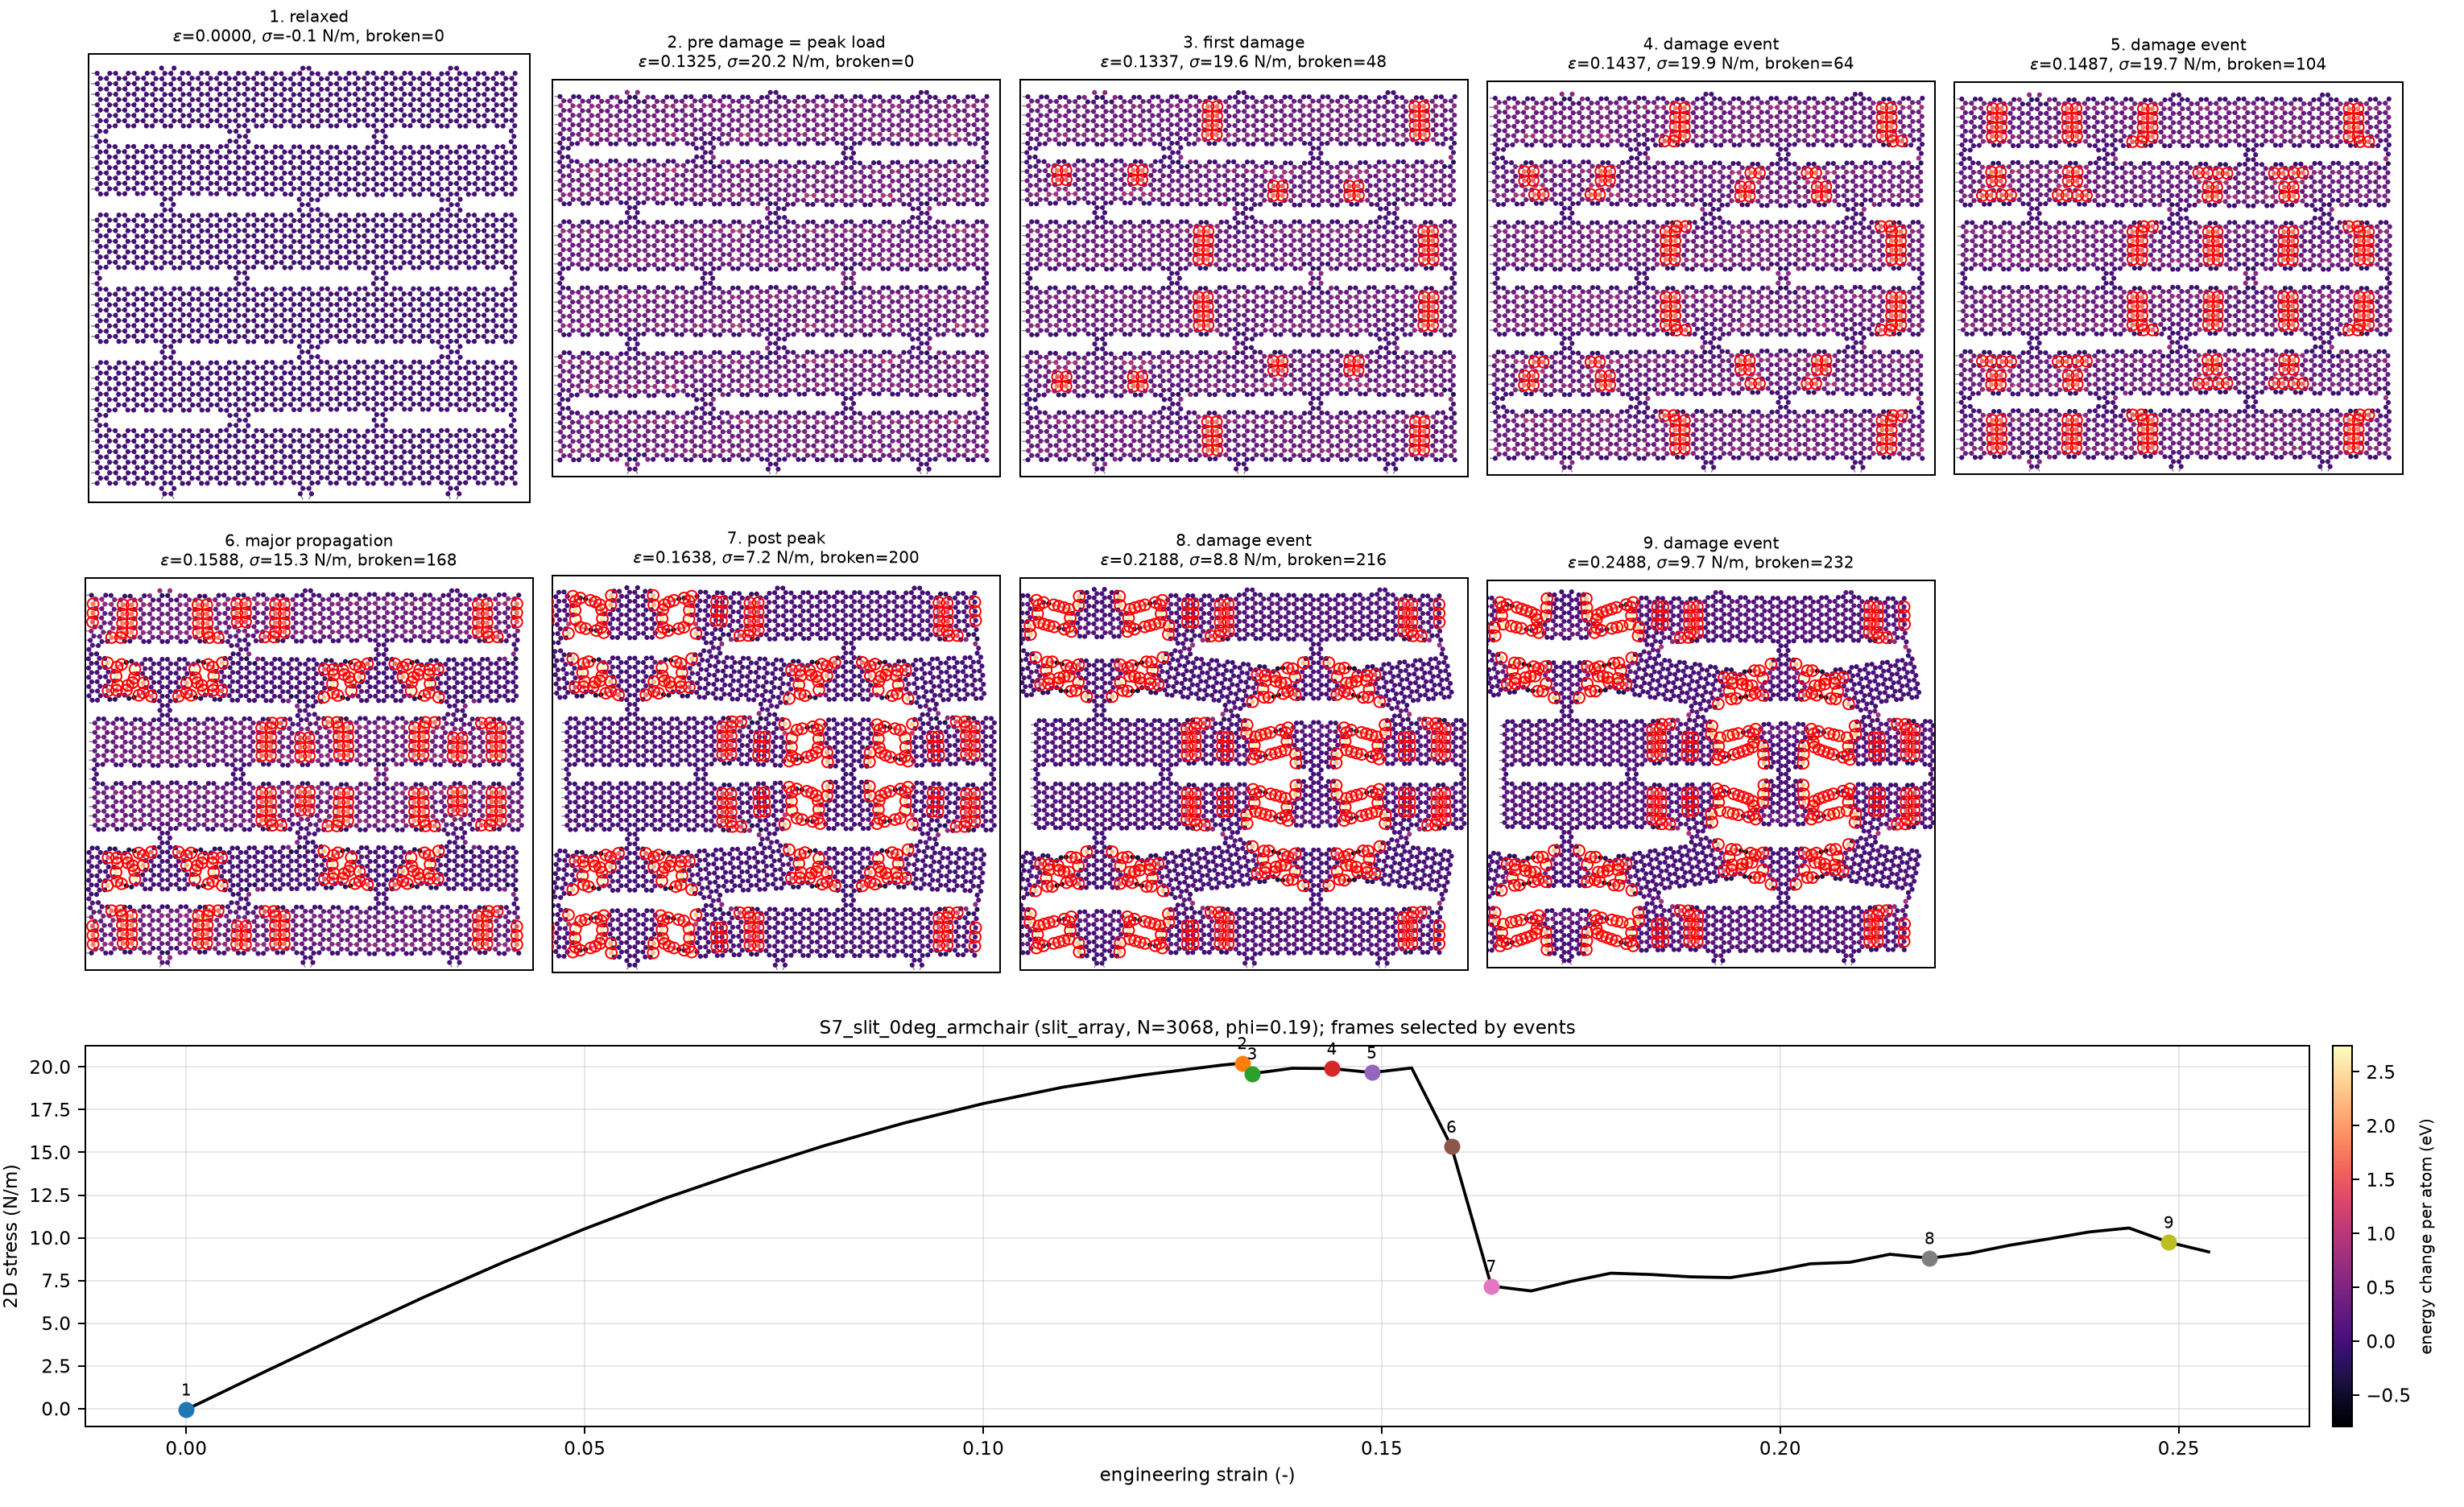
\includegraphics[width=\textwidth]{progression/progression_S7_slit_0deg_armchair_energy_rel.png}\caption{Fracture progression of S7\_slit\_0deg\_armchair (slit\_array, N=3068, porosity 0.19): event-selected frames (relaxed, pre-damage, first bond loss, peak load, major propagation, post-peak, final; colour = energy change per atom relative to the relaxed state, red circles = atoms that lost a bond) and the stress-strain curve with the displayed frames marked.}\label{fig:top3}\end{figure}
Holdout. The parallel slit array of Stage 2 cut from armchair-oriented graphene, so that the load-bearing strips are loaded along their armchair direction. Strength 20.2 N/m, 20\% below the zigzag array (25.4 N/m), in the ratio of the intrinsic armchair and zigzag strengths (30.7/38.8): the ligament strength inherits the chirality of the sheet, which the data-driven predictor (24.0 N/m) did not know. The failure is the most delocalised of the study (L = 0.11): small clusters of broken bonds nucleate inside every strip at the same strain (13.4\%, frames 3-5) without separating the strips, the strips then fail one after another instead of in one avalanche (frame 6, 15.3 N/m with 168 broken bonds), and the sheet retains 8-10 N/m to 25\% strain. Its work to failure (3.0 J/m2) is close to that of the zigzag array despite the lower strength.

\begin{figure}[H]\centering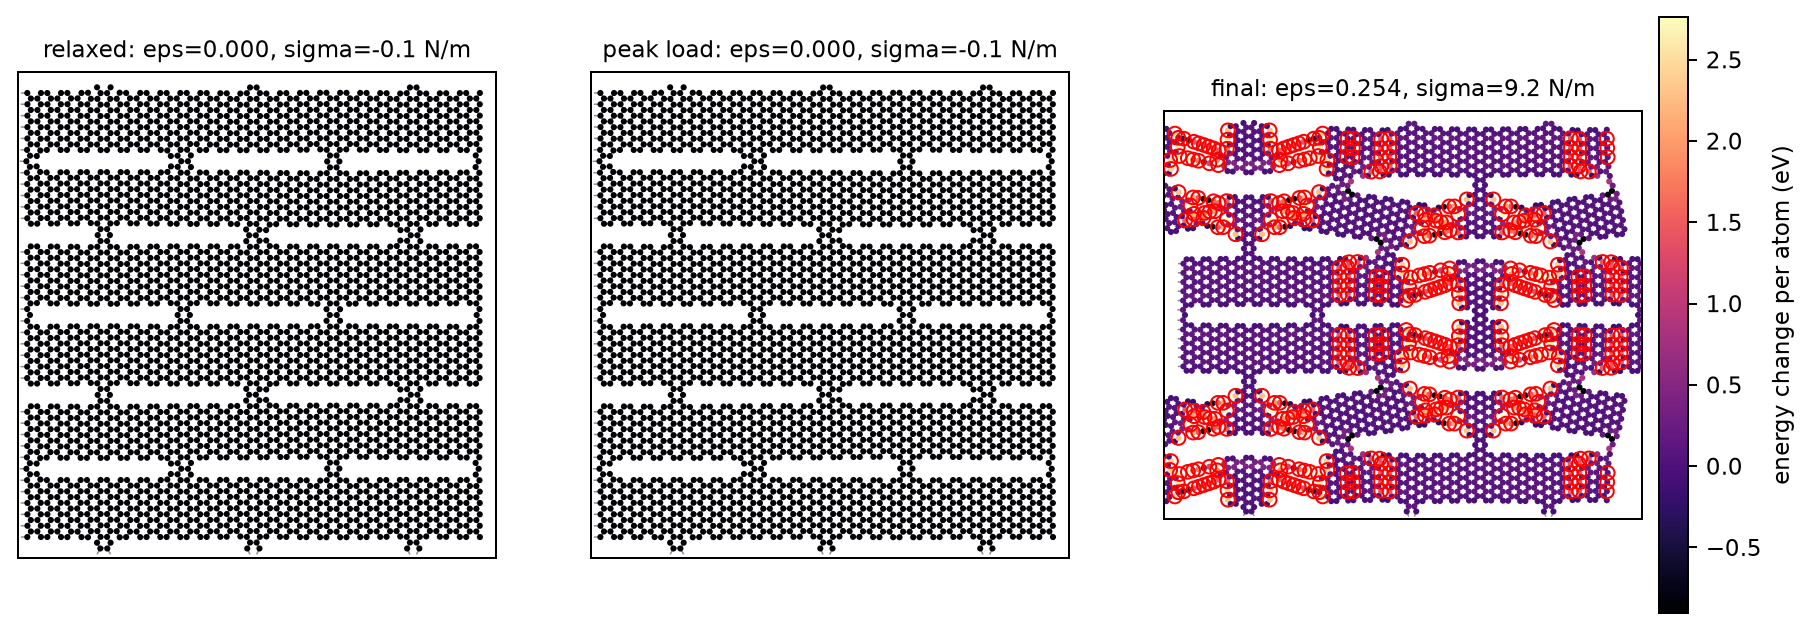
\includegraphics[width=0.95\textwidth]{progression/before_after_S7_slit_0deg_armchair.png}\caption{Before/after comparison for Most delocalised / progressive fracture: relaxed, peak load and final configuration (colour: energy change per atom; red circles: atoms that lost a bond).}\end{figure}

\subsection{Most localised fracture}
\begin{figure}[H]\centering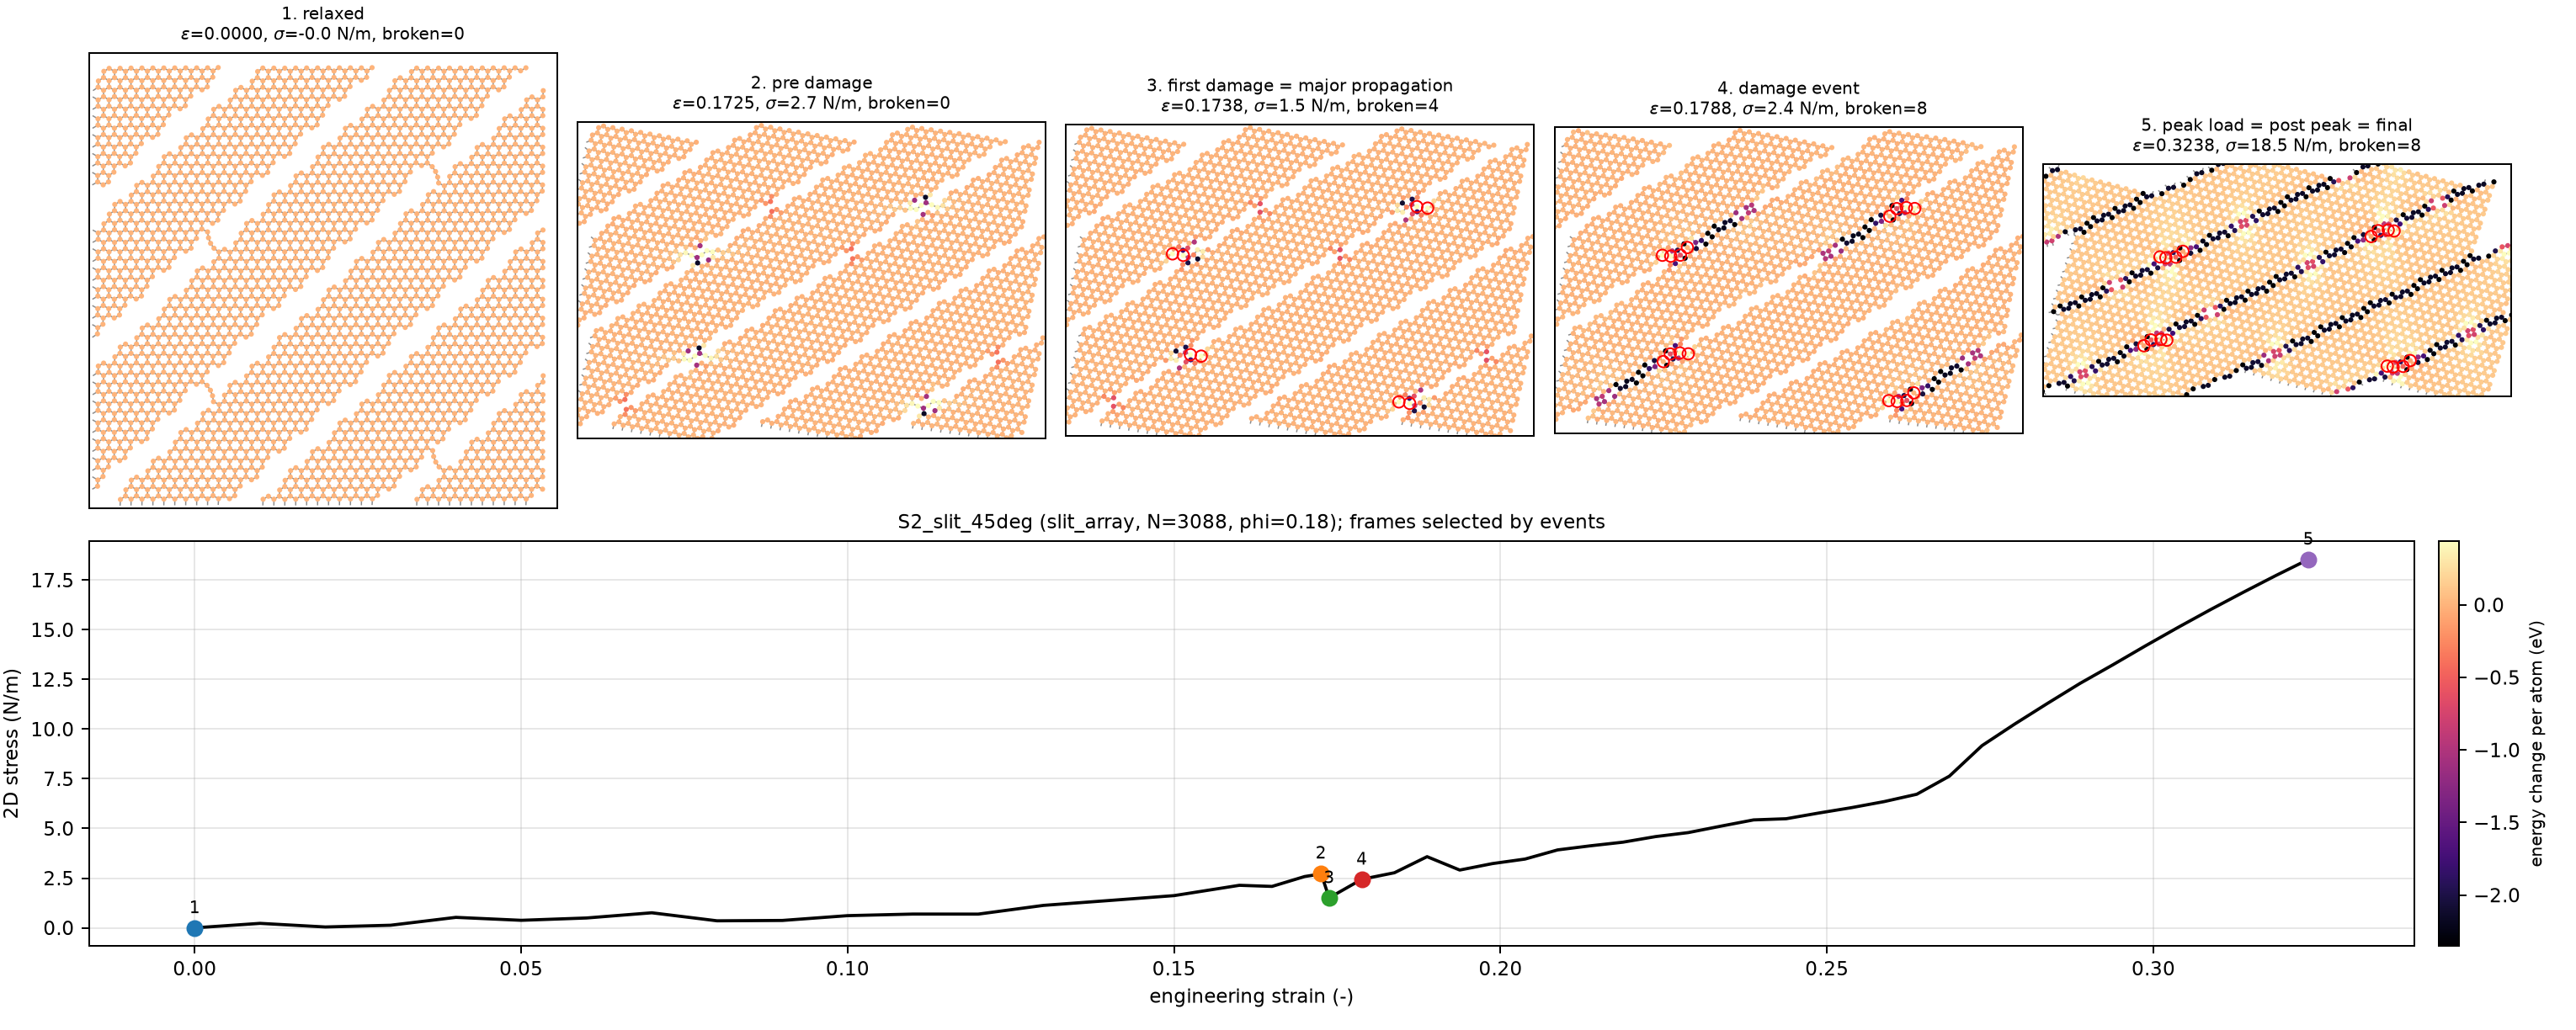
\includegraphics[width=\textwidth]{progression/progression_S2_slit_45deg_energy_rel.png}\caption{Fracture progression of S2\_slit\_45deg (slit\_array, N=3088, porosity 0.18): event-selected frames (relaxed, pre-damage, first bond loss, peak load, major propagation, post-peak, final; colour = energy change per atom relative to the relaxed state, red circles = atoms that lost a bond) and the stress-strain curve with the displayed frames marked.}\label{fig:top4}\end{figure}
Unexpected mechanism. Slits at 45 degrees to the load produce a shear-like ligament network that is extremely compliant at first (the ligaments rotate toward the load), sheds load at 17\% strain in a localised event (L = 0.62) and then re-stiffens as the rotated ligaments align, carrying more than 15 N/m again at 30\% strain without breaking further. It reaches the 32\% strain limit intact: geometric compliance converts an early localised failure into the largest failure strain of the study.

\begin{figure}[H]\centering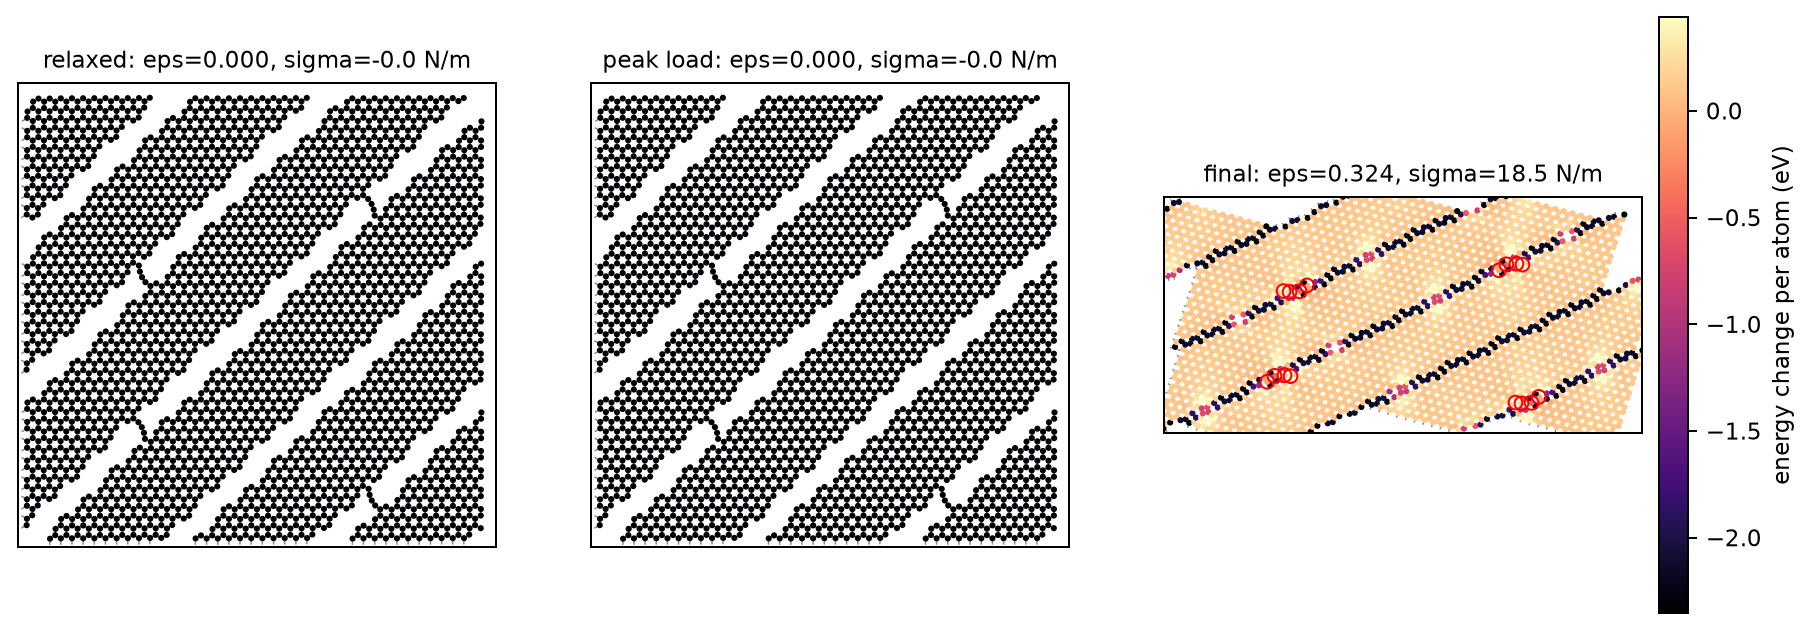
\includegraphics[width=0.95\textwidth]{progression/before_after_S2_slit_45deg.png}\caption{Before/after comparison for Most localised fracture: relaxed, peak load and final configuration (colour: energy change per atom; red circles: atoms that lost a bond).}\end{figure}

\subsection{Key hierarchical design}
\begin{figure}[H]\centering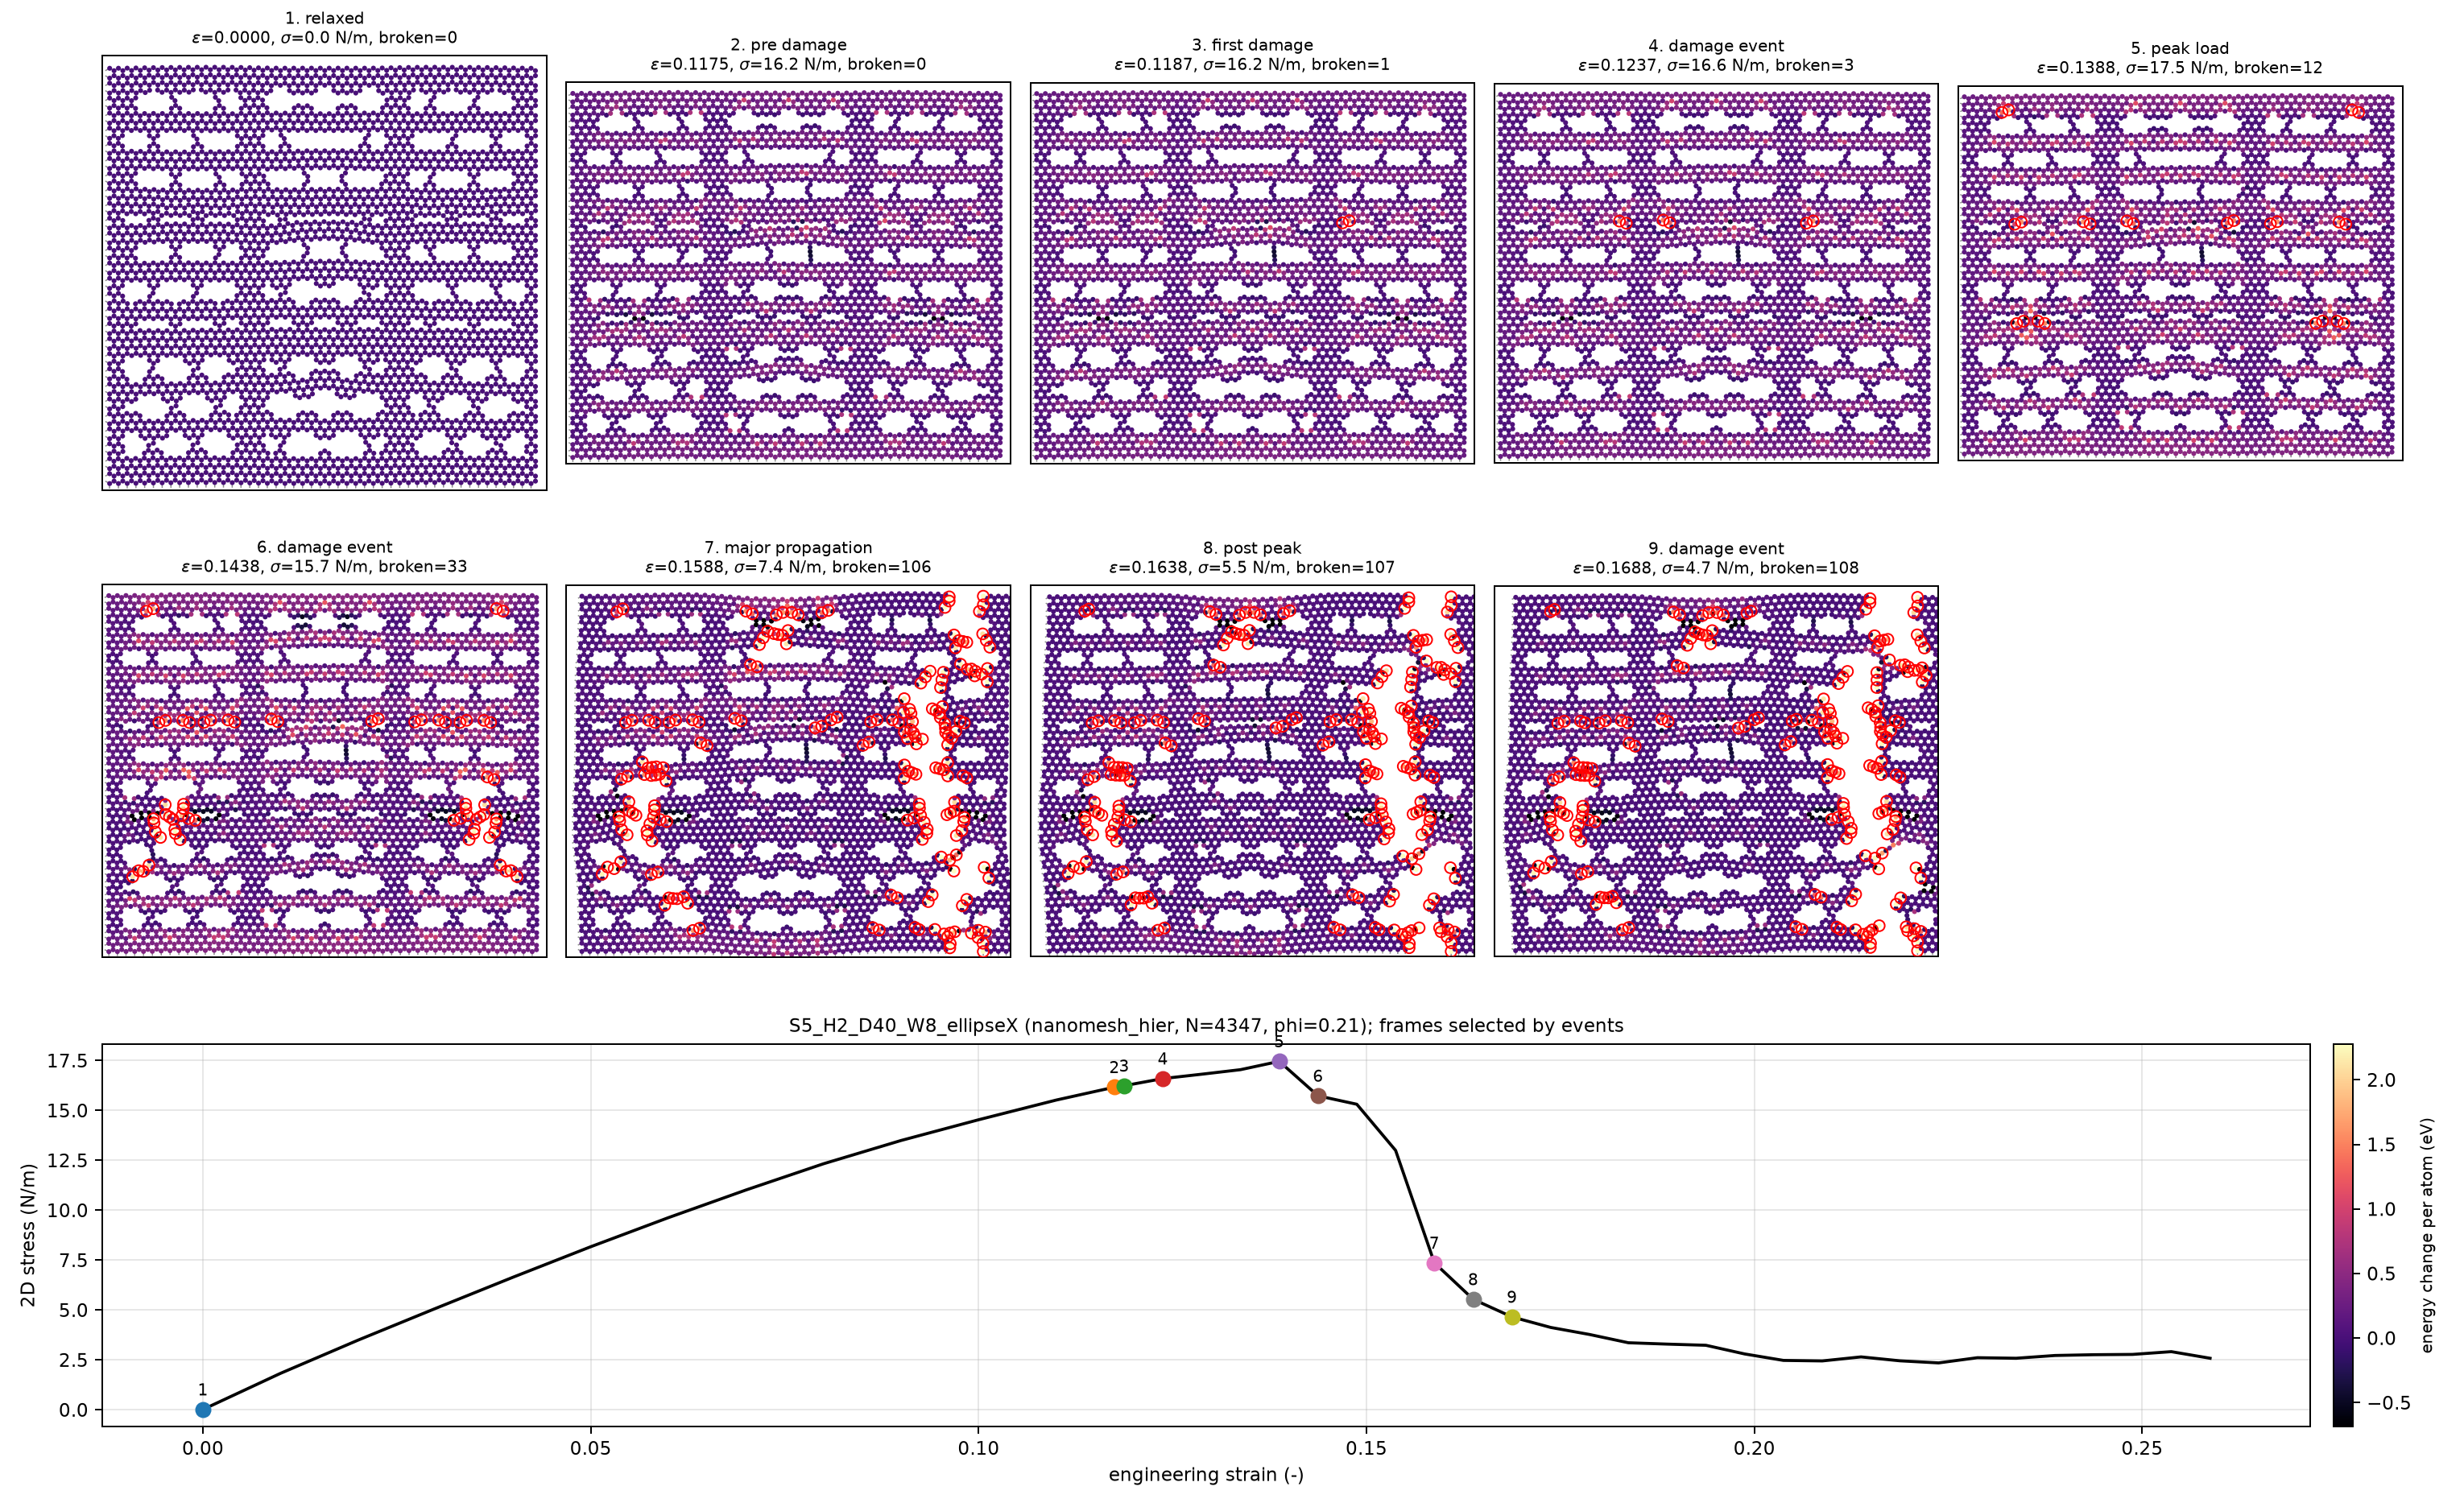
\includegraphics[width=\textwidth]{progression/progression_S5_H2_D40_W8_ellipseX_energy_rel.png}\caption{Fracture progression of S5\_H2\_D40\_W8\_ellipseX (nanomesh\_hier, N=4347, porosity 0.21): event-selected frames (relaxed, pre-damage, first bond loss, peak load, major propagation, post-peak, final; colour = energy change per atom relative to the relaxed state, red circles = atoms that lost a bond) and the stress-strain curve with the displayed frames marked.}\label{fig:top5}\end{figure}
Key hierarchical design and the only nested mesh that beats the coarse-only limit: fine pores elongated along the load inside a vein network give 17.5 N/m, W = 2.0 J/m2 and progressive failure over 13\% of post-peak strain. The fine level fails first at the pore ends, but because the fine ligaments are straight (high net-section strength) and numerous (fibre-bundle load sharing), the load transfers to neighbouring rows and the load-parallel veins instead of cascading. Hierarchy is beneficial here only because both levels are aligned with the load.

\begin{figure}[H]\centering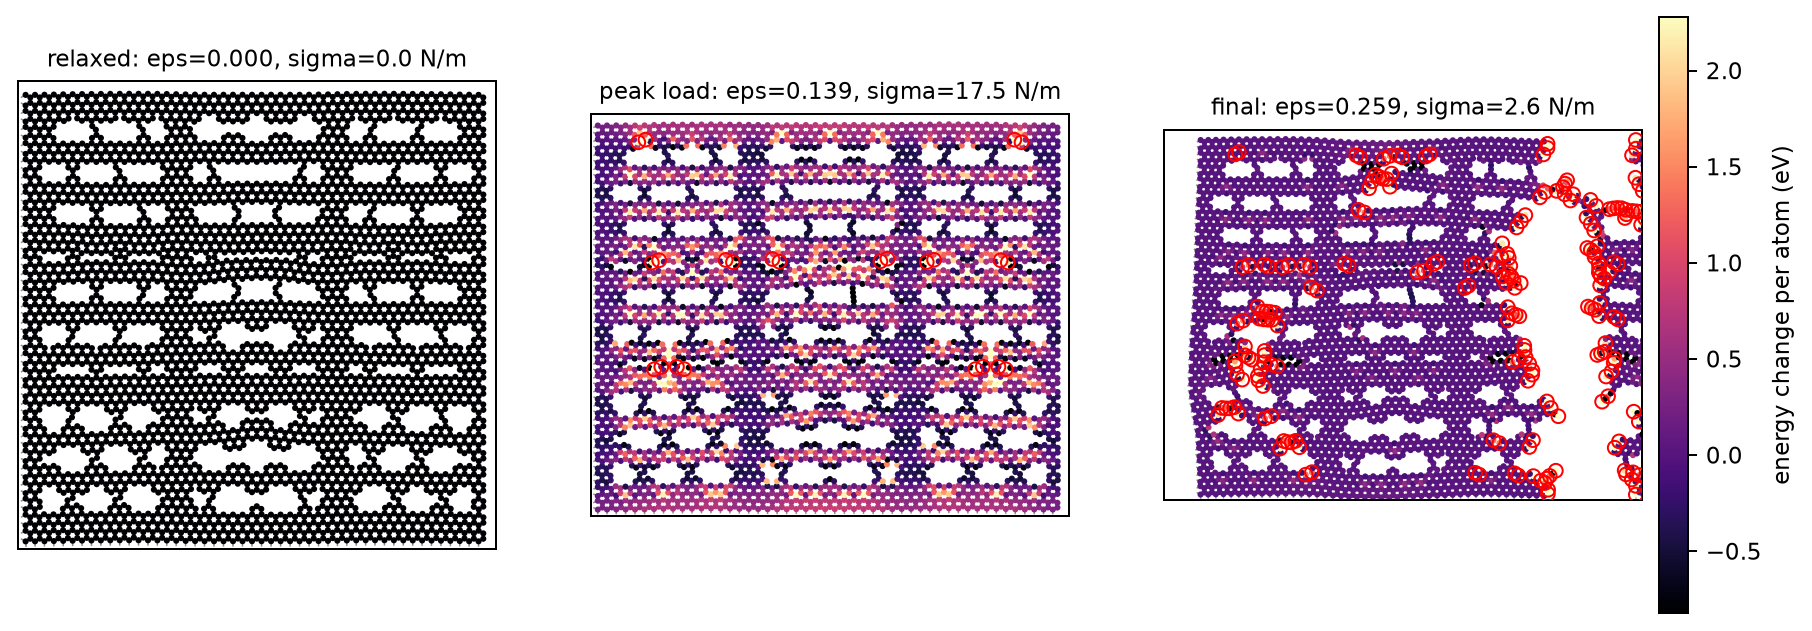
\includegraphics[width=0.95\textwidth]{progression/before_after_S5_H2_D40_W8_ellipseX.png}\caption{Before/after comparison for Key hierarchical design: relaxed, peak load and final configuration (colour: energy change per atom; red circles: atoms that lost a bond).}\end{figure}

\subsection{Flaw-halo design (hole + pore rings)}
\begin{figure}[H]\centering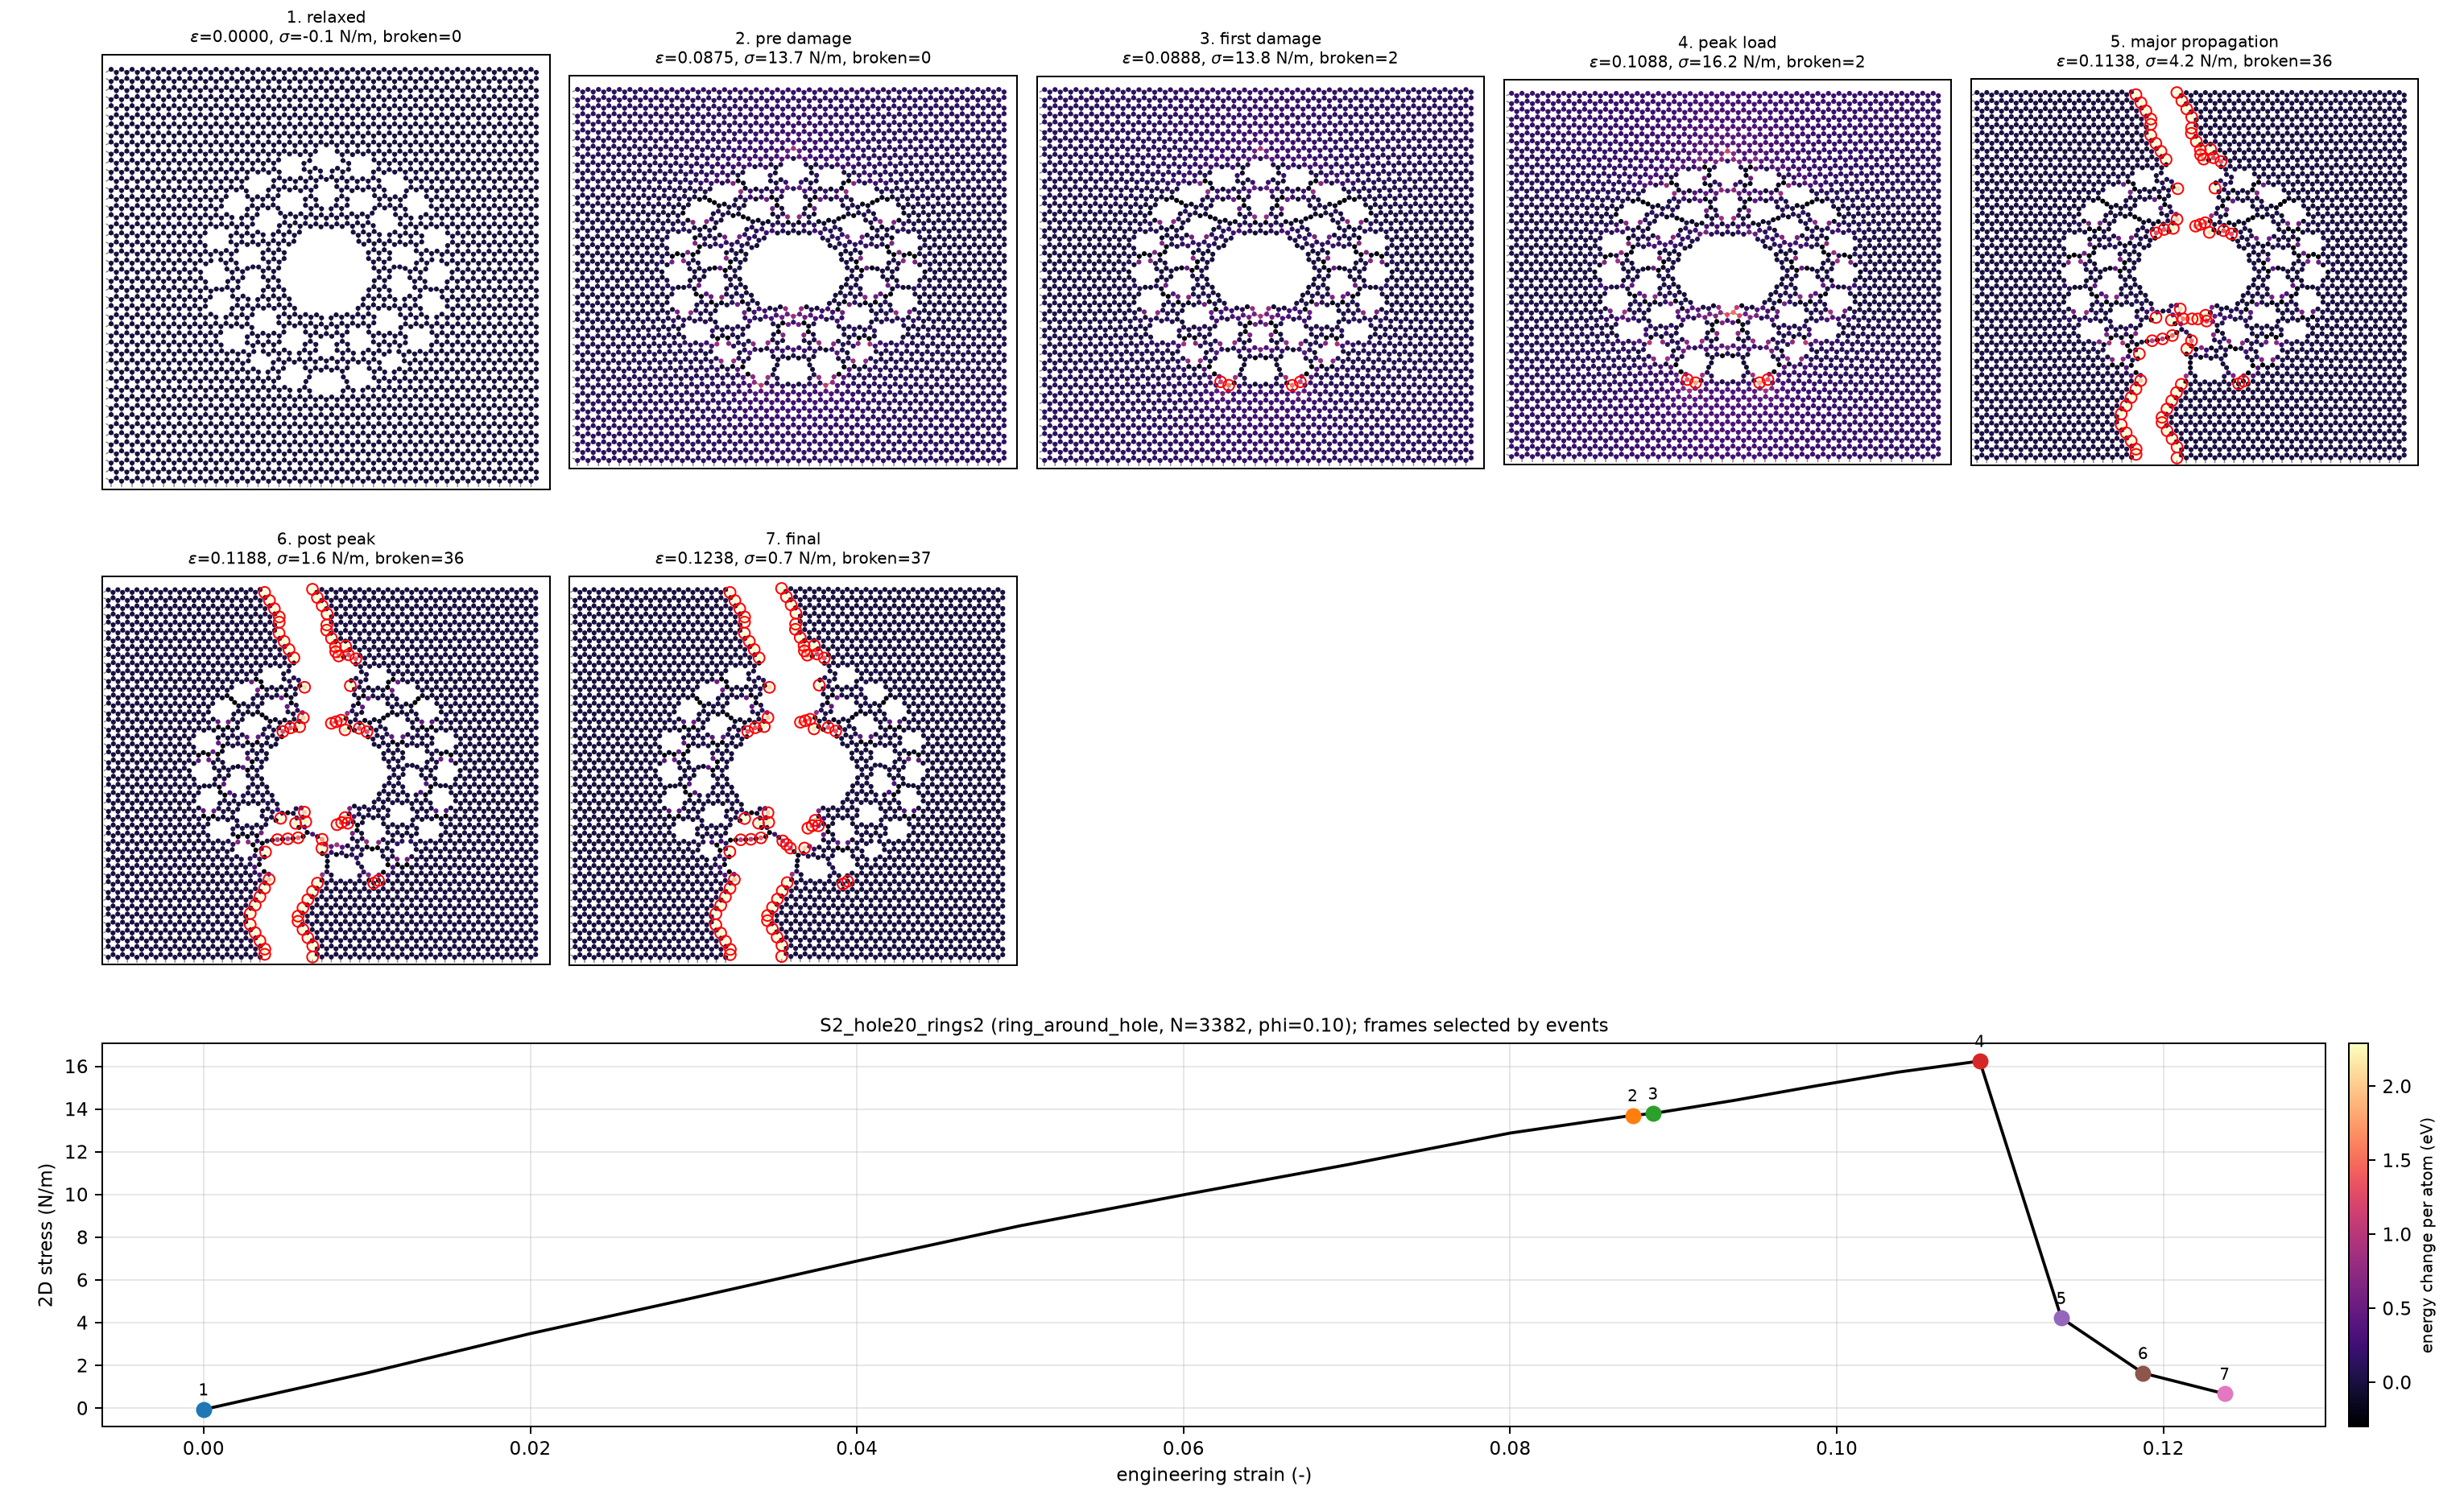
\includegraphics[width=\textwidth]{progression/progression_S2_hole20_rings2_energy_rel.png}\caption{Fracture progression of S2\_hole20\_rings2 (ring\_around\_hole, N=3382, porosity 0.10): event-selected frames (relaxed, pre-damage, first bond loss, peak load, major propagation, post-peak, final; colour = energy change per atom relative to the relaxed state, red circles = atoms that lost a bond) and the stress-strain curve with the displayed frames marked.}\label{fig:top6}\end{figure}
Flaw halo. Two rings of 5 A pores around a 20 A hole: the sheet reaches 16.2 N/m, below the bare hole (19.1) but above the same porosity spread uniformly in the far field (13.2). Damage starts at the hole edge, not in the halo, and the halo pores merely provide a compliant path for the crack. The halo does not shield the flaw; it only localises the penalty of the added porosity, so the 'nested rings around a void' motif of the reference images is a cost, not a toughening mechanism, in this model.

\begin{figure}[H]\centering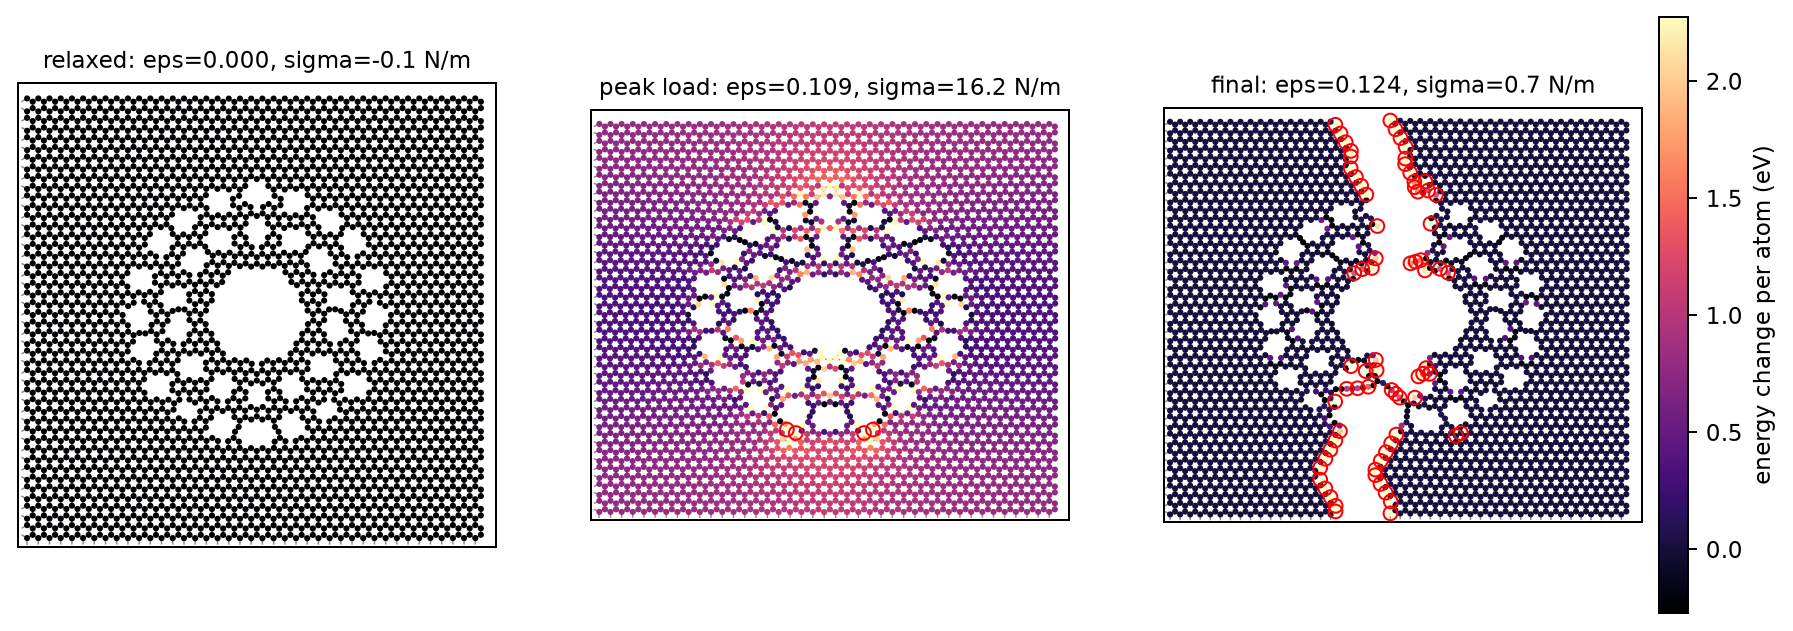
\includegraphics[width=0.95\textwidth]{progression/before_after_S2_hole20_rings2.png}\caption{Before/after comparison for Flaw-halo design (hole + pore rings): relaxed, peak load and final configuration (colour: energy change per atom; red circles: atoms that lost a bond).}\end{figure}

\subsection{Counter-example within the hierarchy ladder}
\begin{figure}[H]\centering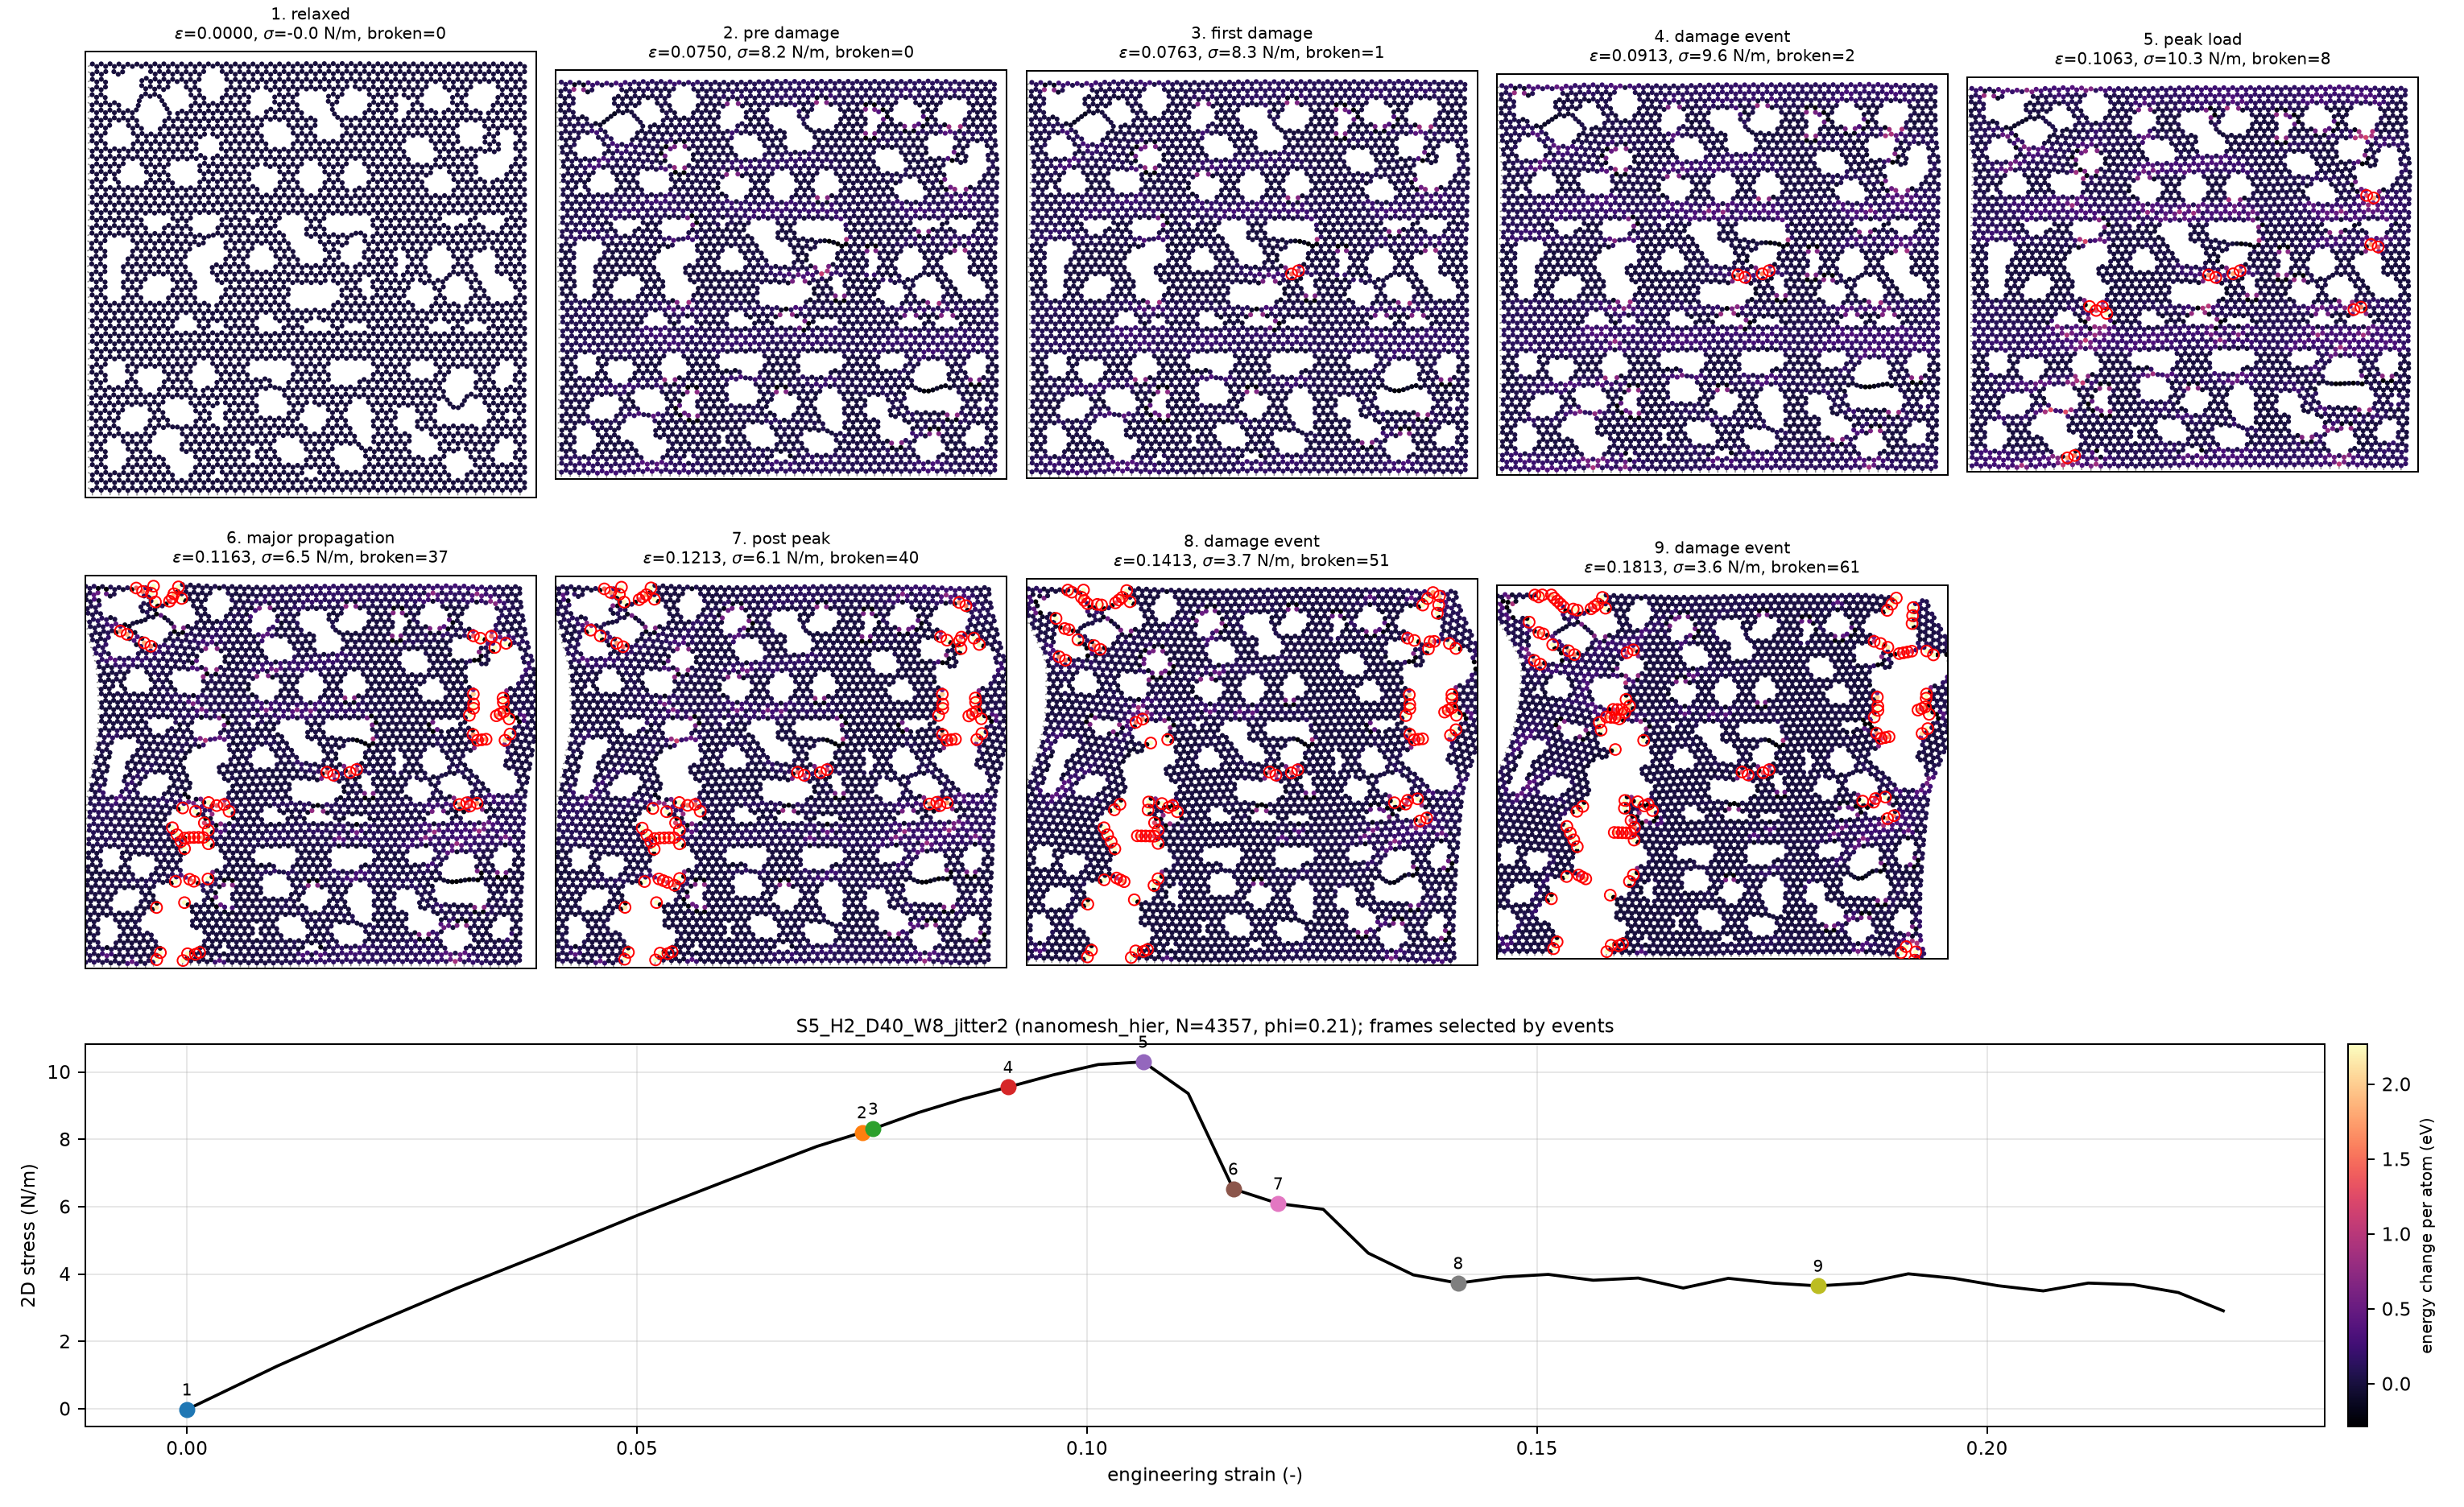
\includegraphics[width=\textwidth]{progression/progression_S5_H2_D40_W8_jitter2_energy_rel.png}\caption{Fracture progression of S5\_H2\_D40\_W8\_jitter2 (nanomesh\_hier, N=4357, porosity 0.21): event-selected frames (relaxed, pre-damage, first bond loss, peak load, major propagation, post-peak, final; colour = energy change per atom relative to the relaxed state, red circles = atoms that lost a bond) and the stress-strain curve with the displayed frames marked.}\label{fig:top7}\end{figure}
Counter-example. Disordering the fine level of the two-level mesh (2 A jitter) lowers its strength from 12.8 to 10.3 N/m, the same penalty disorder inflicts on a single-scale mesh, and the veins do not compensate: the first bonds break at the most misaligned fine ligament and the damage spreads through the domain before the veins carry the load. Hierarchy and disorder do not interact favourably.

\begin{figure}[H]\centering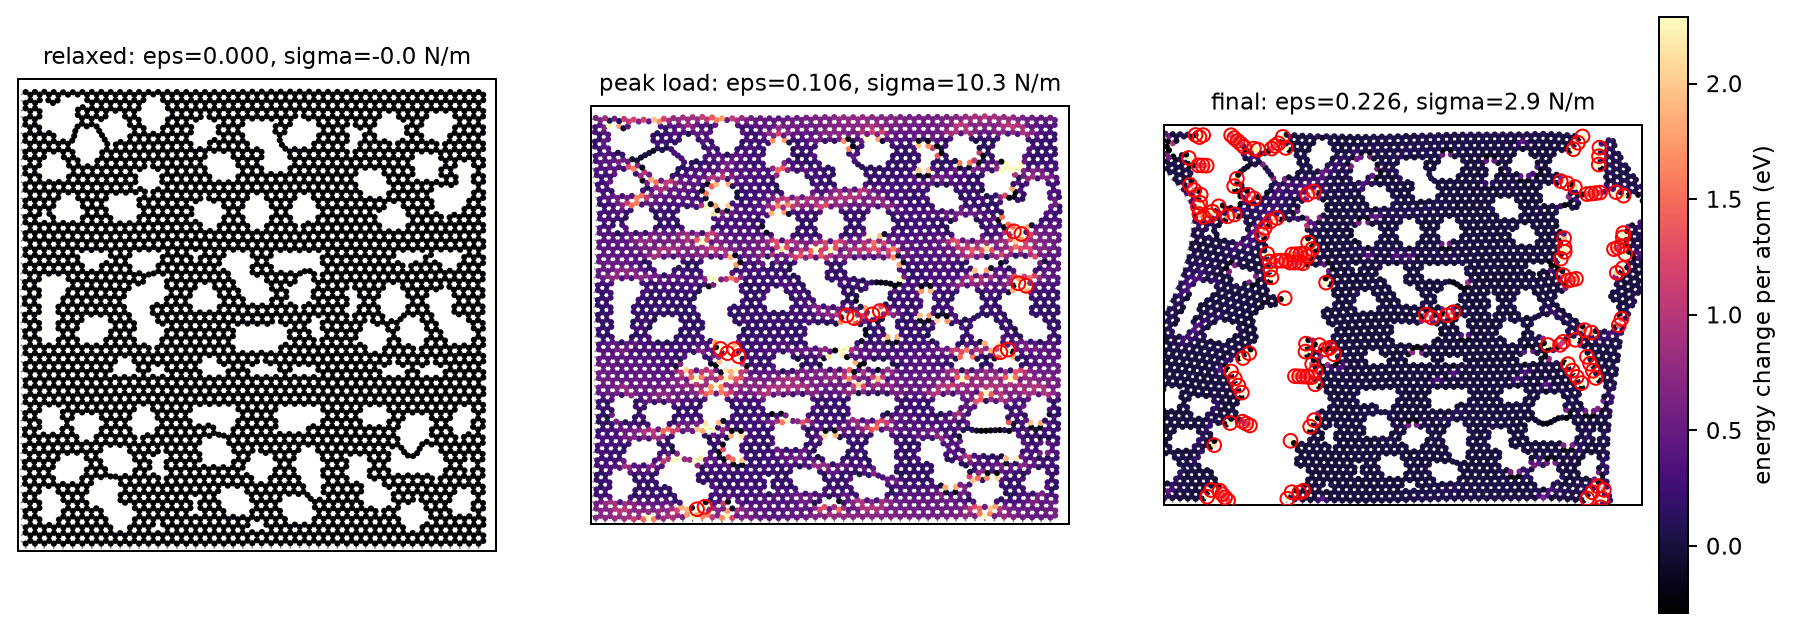
\includegraphics[width=0.95\textwidth]{progression/before_after_S5_H2_D40_W8_jitter2.png}\caption{Before/after comparison for Counter-example within the hierarchy ladder: relaxed, peak load and final configuration (colour: energy change per atom; red circles: atoms that lost a bond).}\end{figure}

\subsection{Holdout: load-aligned veins + load-aligned ellipses}
\begin{figure}[H]\centering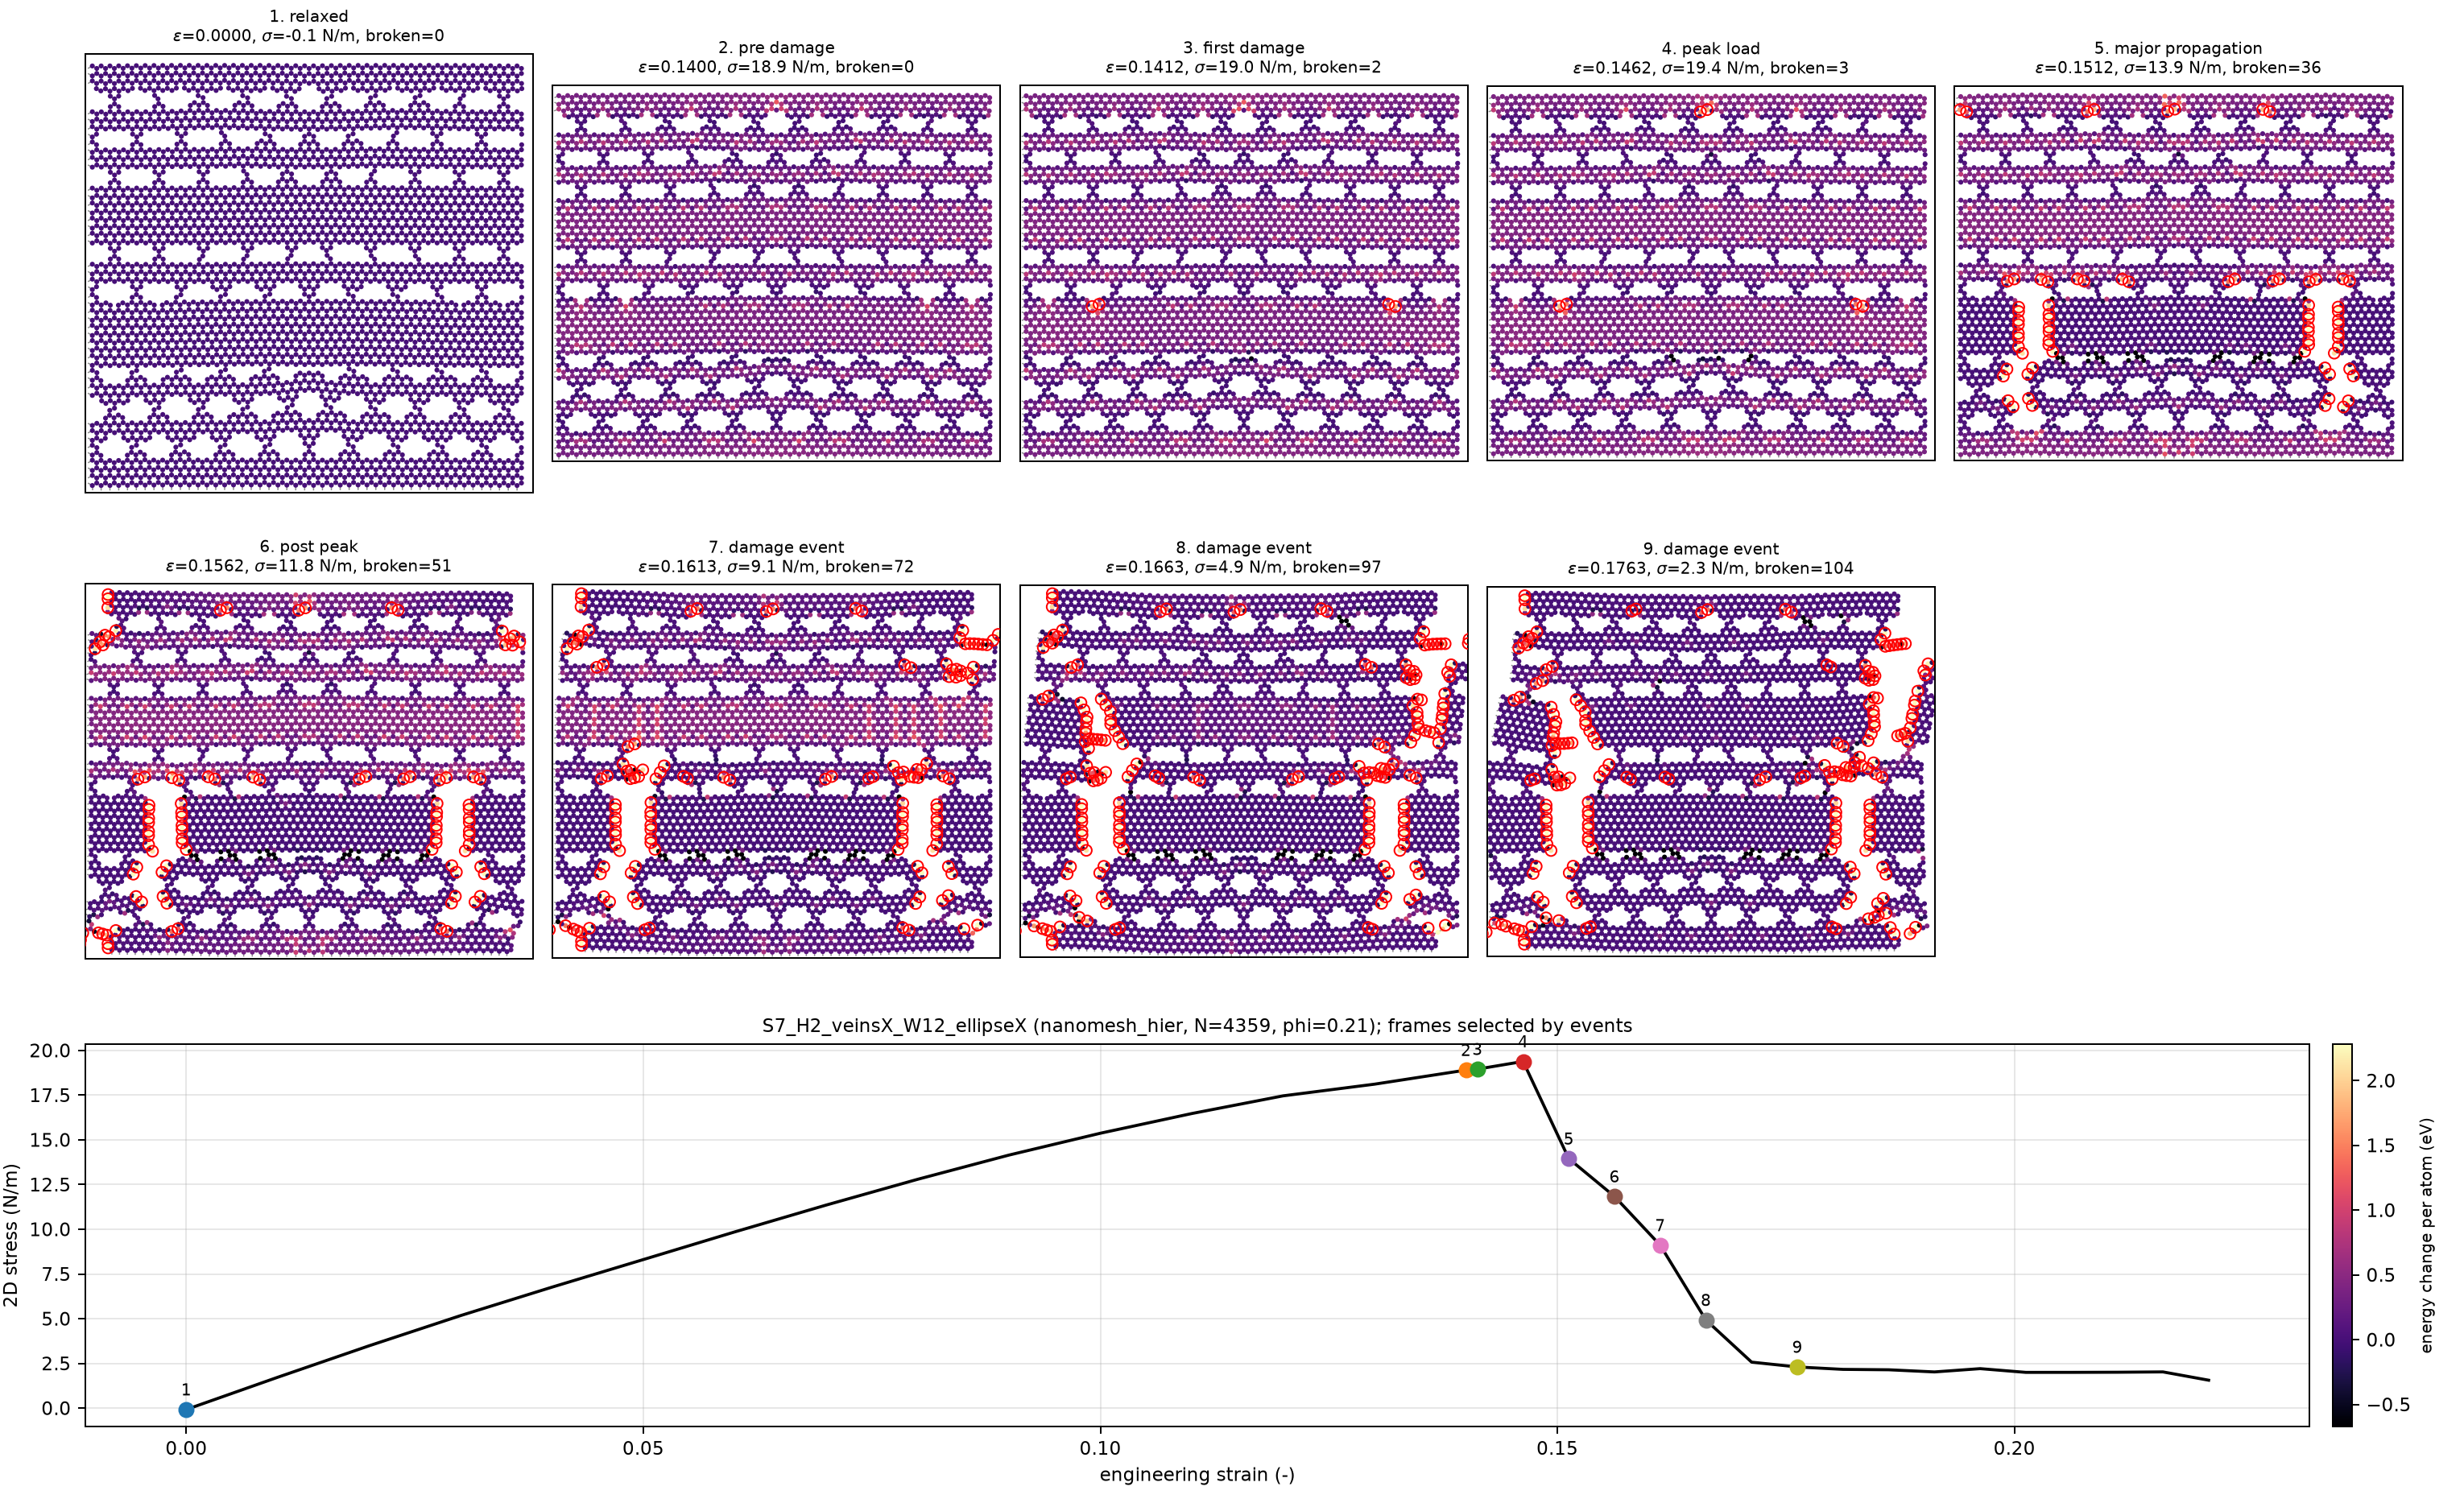
\includegraphics[width=\textwidth]{progression/progression_S7_H2_veinsX_W12_ellipseX_energy_rel.png}\caption{Fracture progression of S7\_H2\_veinsX\_W12\_ellipseX (nanomesh\_hier, N=4359, porosity 0.21): event-selected frames (relaxed, pre-damage, first bond loss, peak load, major propagation, post-peak, final; colour = energy change per atom relative to the relaxed state, red circles = atoms that lost a bond) and the stress-strain curve with the displayed frames marked.}\label{fig:top8}\end{figure}
Holdout that combines the two alignment effects found separately in Stage 4 (veins only along the load, 16.1 N/m) and Stage 5 (load-elongated fine pores with square veins, 17.5 N/m). With 12 A veins along the load and elliptical fine pores elongated along the load, it is the strongest nested design of the campaign: 19.4 N/m at 20.6\% porosity, above the coarse-only mesh at the same porosity; the data-driven predictor gave 13.3 N/m because it averaged over nested designs with and without alignment. First damage appears at the bridges between the fine pores at 14.1\% strain, the peak follows at 14.6\%, and failure proceeds in a few steps (19.4 to 11.8 N/m at the first event) as the fine-pore rows fail while the veins carry the remaining load; the work to failure (2.0 J/m2) equals that of the Stage 5 aligned mesh. The two alignments act on different length scales and their benefits add.

\begin{figure}[H]\centering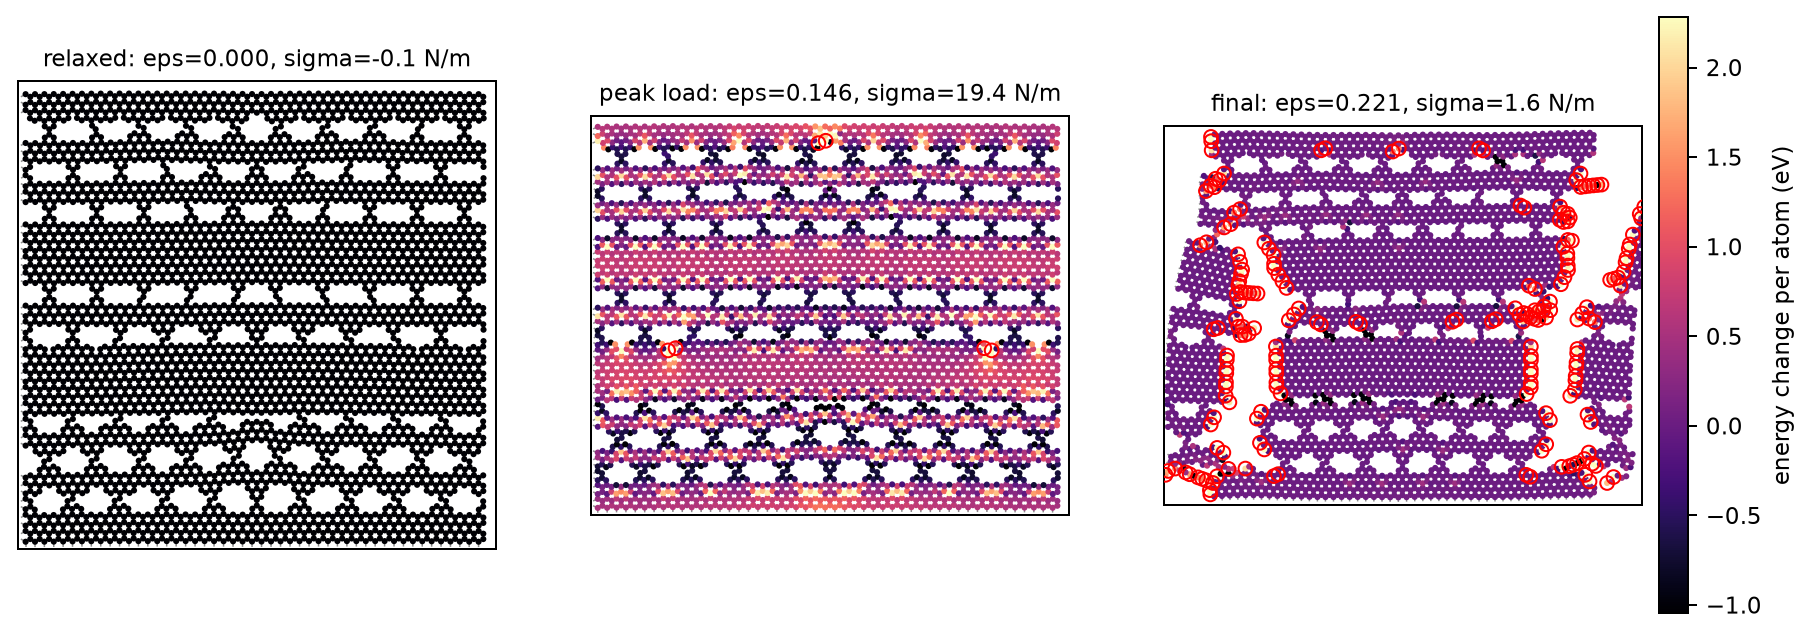
\includegraphics[width=0.95\textwidth]{progression/before_after_S7_H2_veinsX_W12_ellipseX.png}\caption{Before/after comparison for Holdout: load-aligned veins + load-aligned ellipses: relaxed, peak load and final configuration (colour: energy change per atom; red circles: atoms that lost a bond).}\end{figure}

\subsection{Holdout: slit array at 20 degrees (echelon coalescence)}
\begin{figure}[H]\centering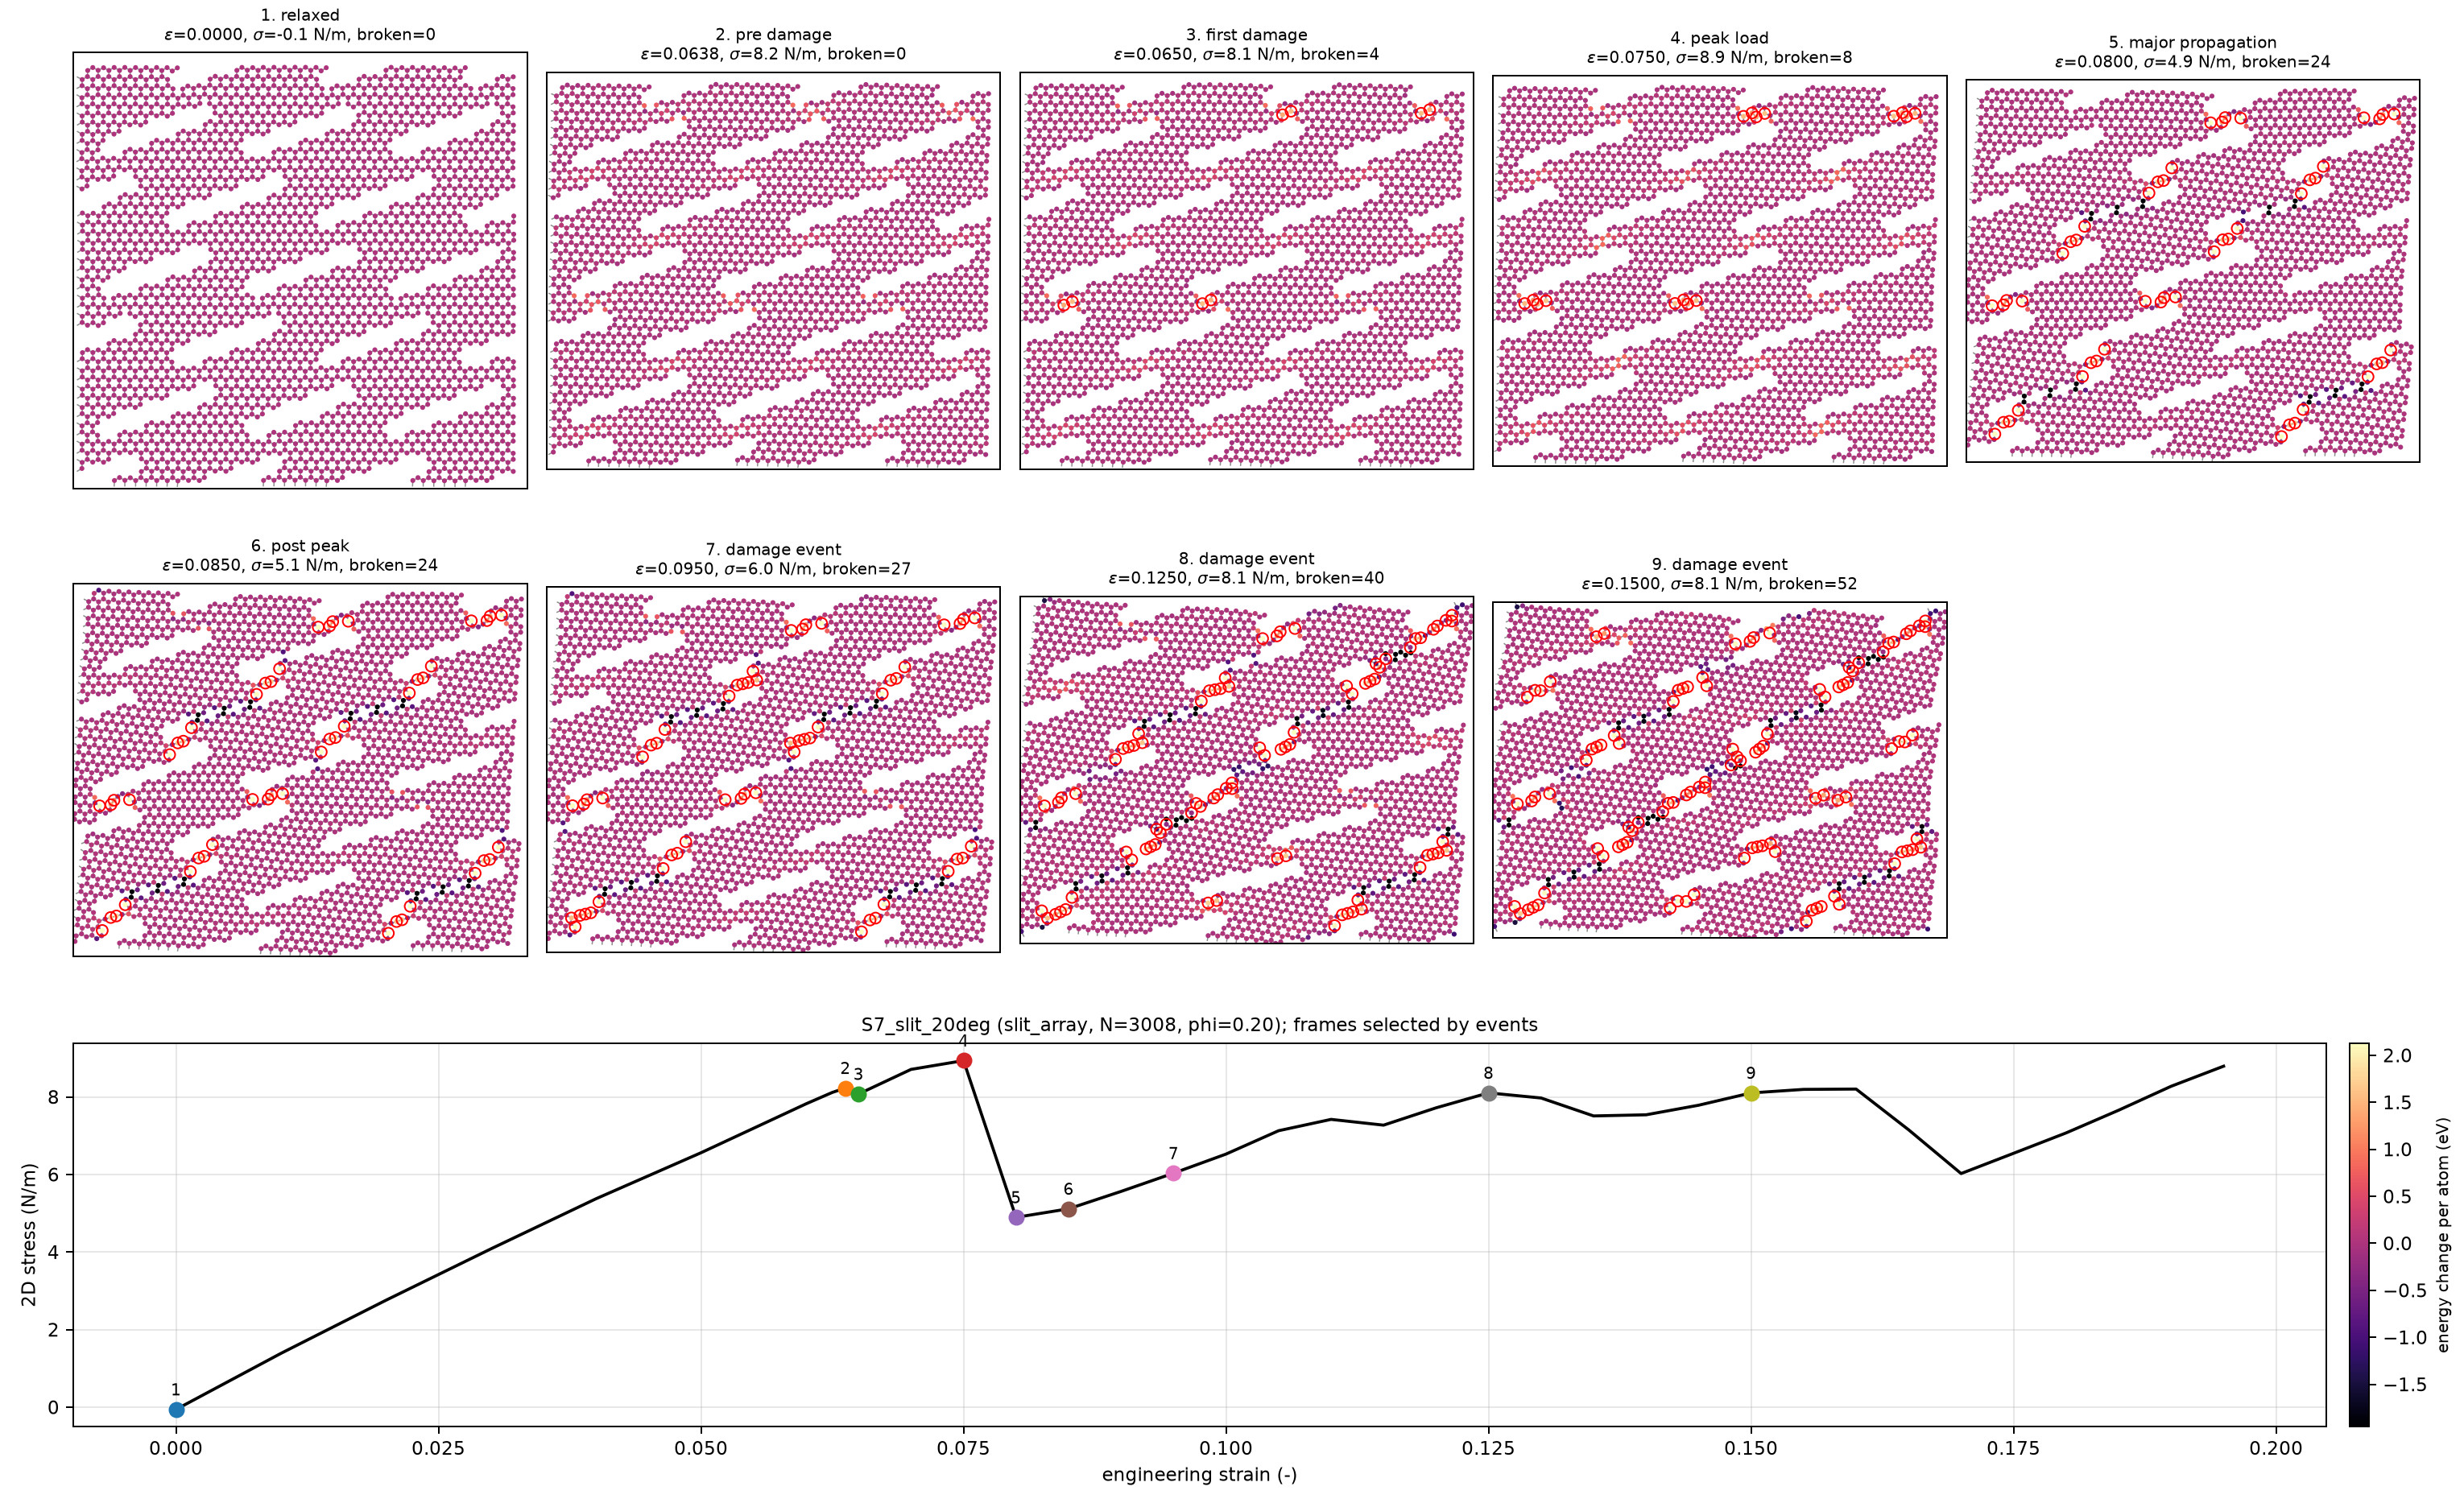
\includegraphics[width=\textwidth]{progression/progression_S7_slit_20deg_energy_rel.png}\caption{Fracture progression of S7\_slit\_20deg (slit\_array, N=3008, porosity 0.20): event-selected frames (relaxed, pre-damage, first bond loss, peak load, major propagation, post-peak, final; colour = energy change per atom relative to the relaxed state, red circles = atoms that lost a bond) and the stress-strain curve with the displayed frames marked.}\label{fig:top9}\end{figure}
Holdout with the largest prediction miss (predicted 23.9 N/m, observed 8.9 N/m). Rotating the parallel slit array by 20 degrees makes the tips of the slits in neighbouring rows overlap along the load; the short inclined ligaments between overlapping tips carry the load in combined shear and tension and fail first (first damage at 6.5\% strain, peak at 7.5\%). Each failed ligament hands its load to the next one along the same inclined path, so the cracks coalesce en echelon across the sheet (post-peak and final frames), while the remaining strips keep carrying about 8 N/m up to 19.5\% strain (progressive mode, L = 0.20). Load-path alignment is therefore not a monotonic function of angle: it is lost as soon as adjacent slit tips overlap, at a strength below even the 45-degree array (18.5 N/m) and closer to the perpendicular array (4.0 N/m).

\begin{figure}[H]\centering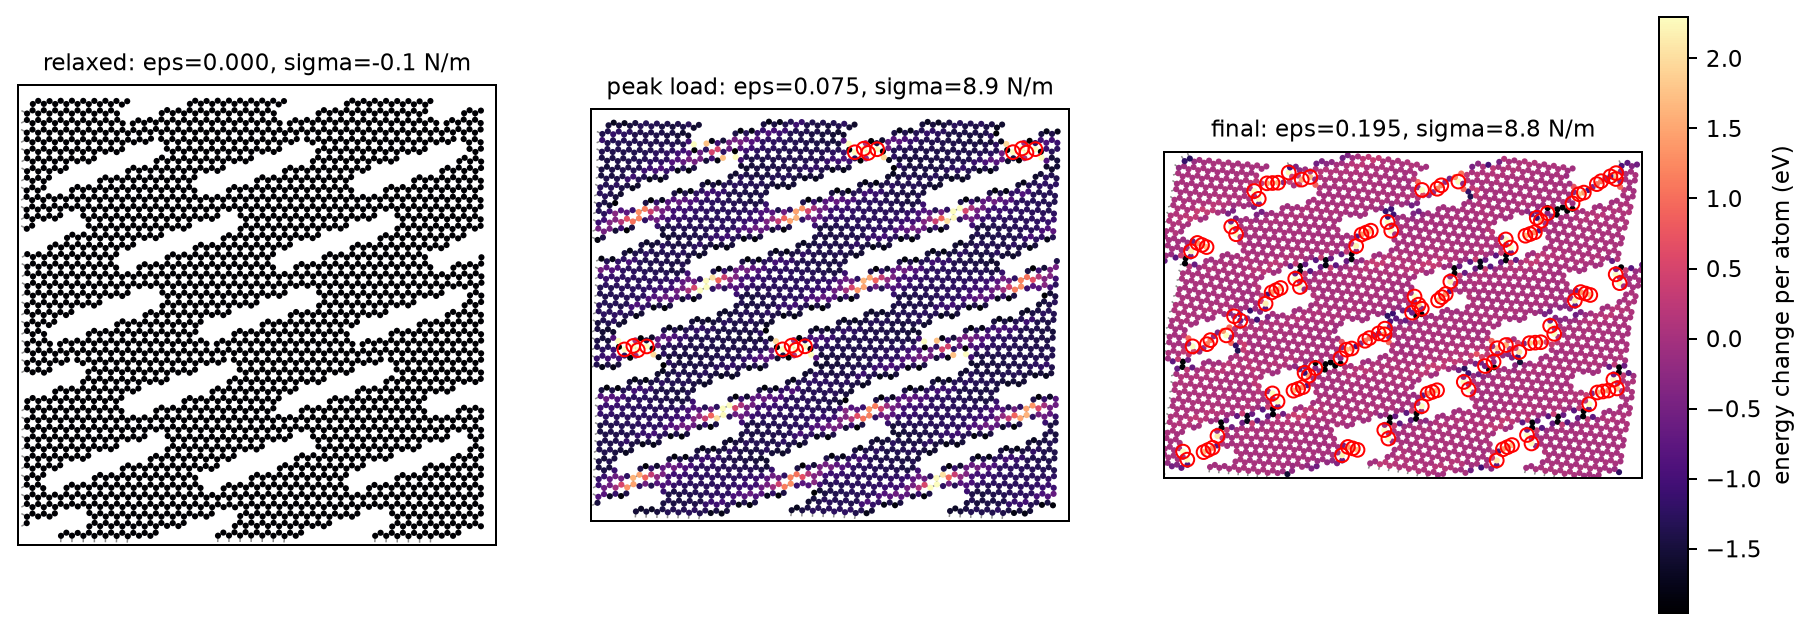
\includegraphics[width=0.95\textwidth]{progression/before_after_S7_slit_20deg.png}\caption{Before/after comparison for Holdout: slit array at 20 degrees (echelon coalescence): relaxed, peak load and final configuration (colour: energy change per atom; red circles: atoms that lost a bond).}\end{figure}

\begin{figure}[H]\centering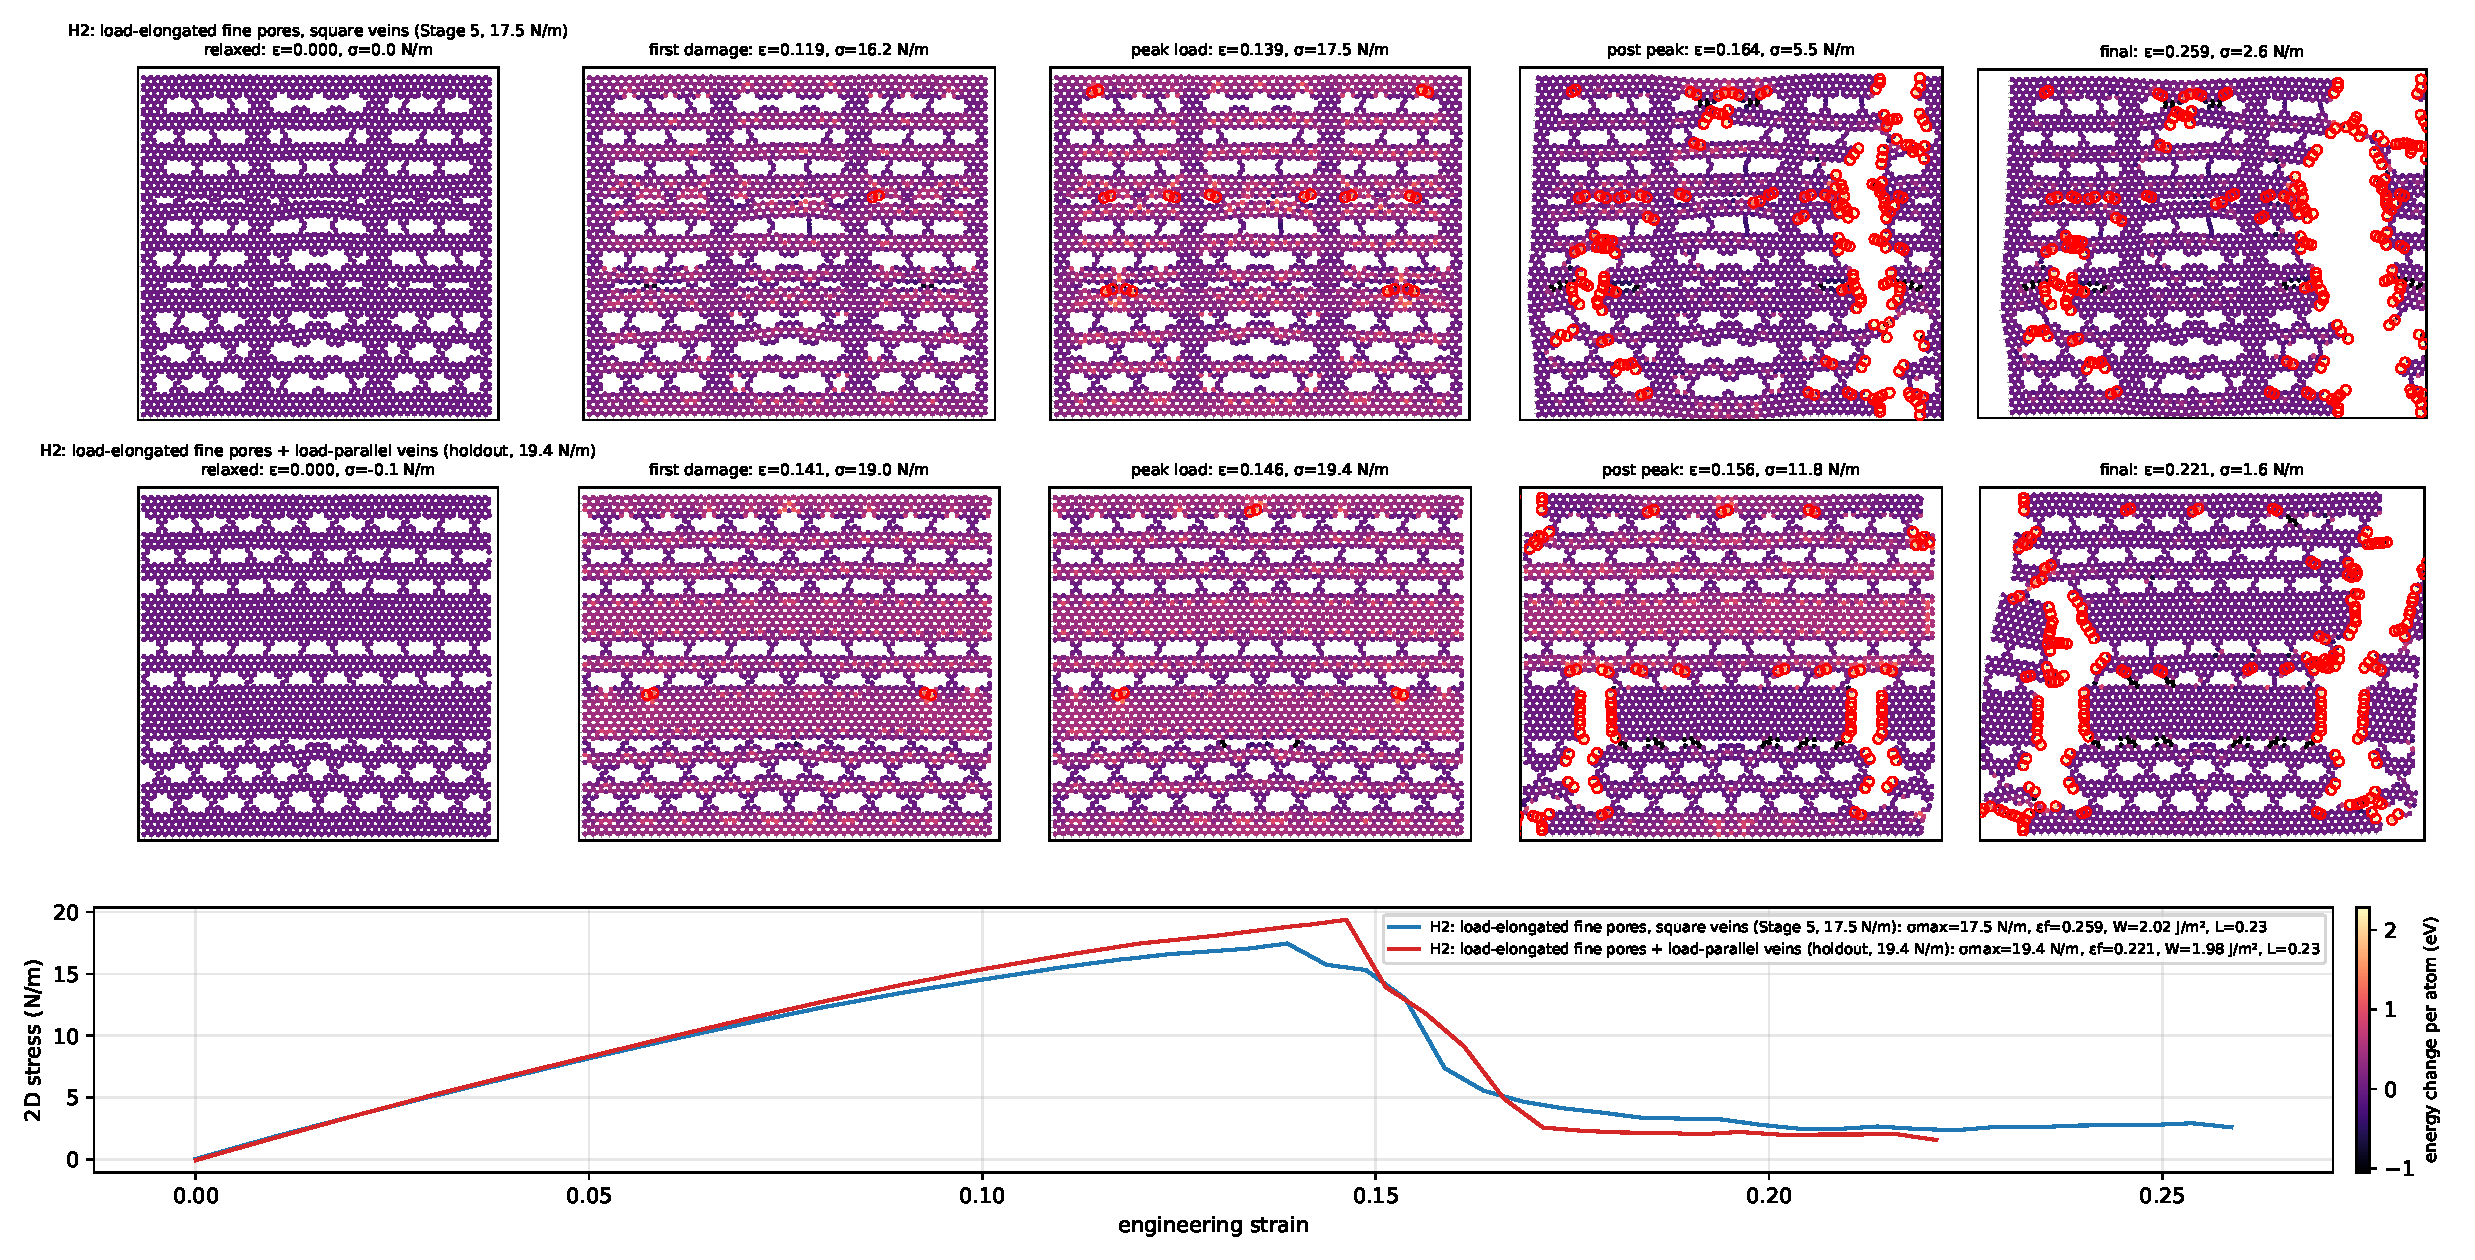
\includegraphics[width=1.0\textwidth]{progression/comparison_aligned_hierarchy_synergy.pdf}\caption{Holdout: combining the two orientation effects (load-elongated fine pores and veins along the load only) gives the strongest nested design of the campaign (19.4 N/m, predicted 13.3 N/m by the data-driven predictor): the two alignments act on different length scales and their benefits add. Rows: relaxed, first damage, peak load, post-peak, final; colour: energy change per atom; bottom: stress-strain curves with the selected events marked.}\label{fig:comparison_aligned_hierarchy_synergy}\end{figure}
\begin{figure}[H]\centering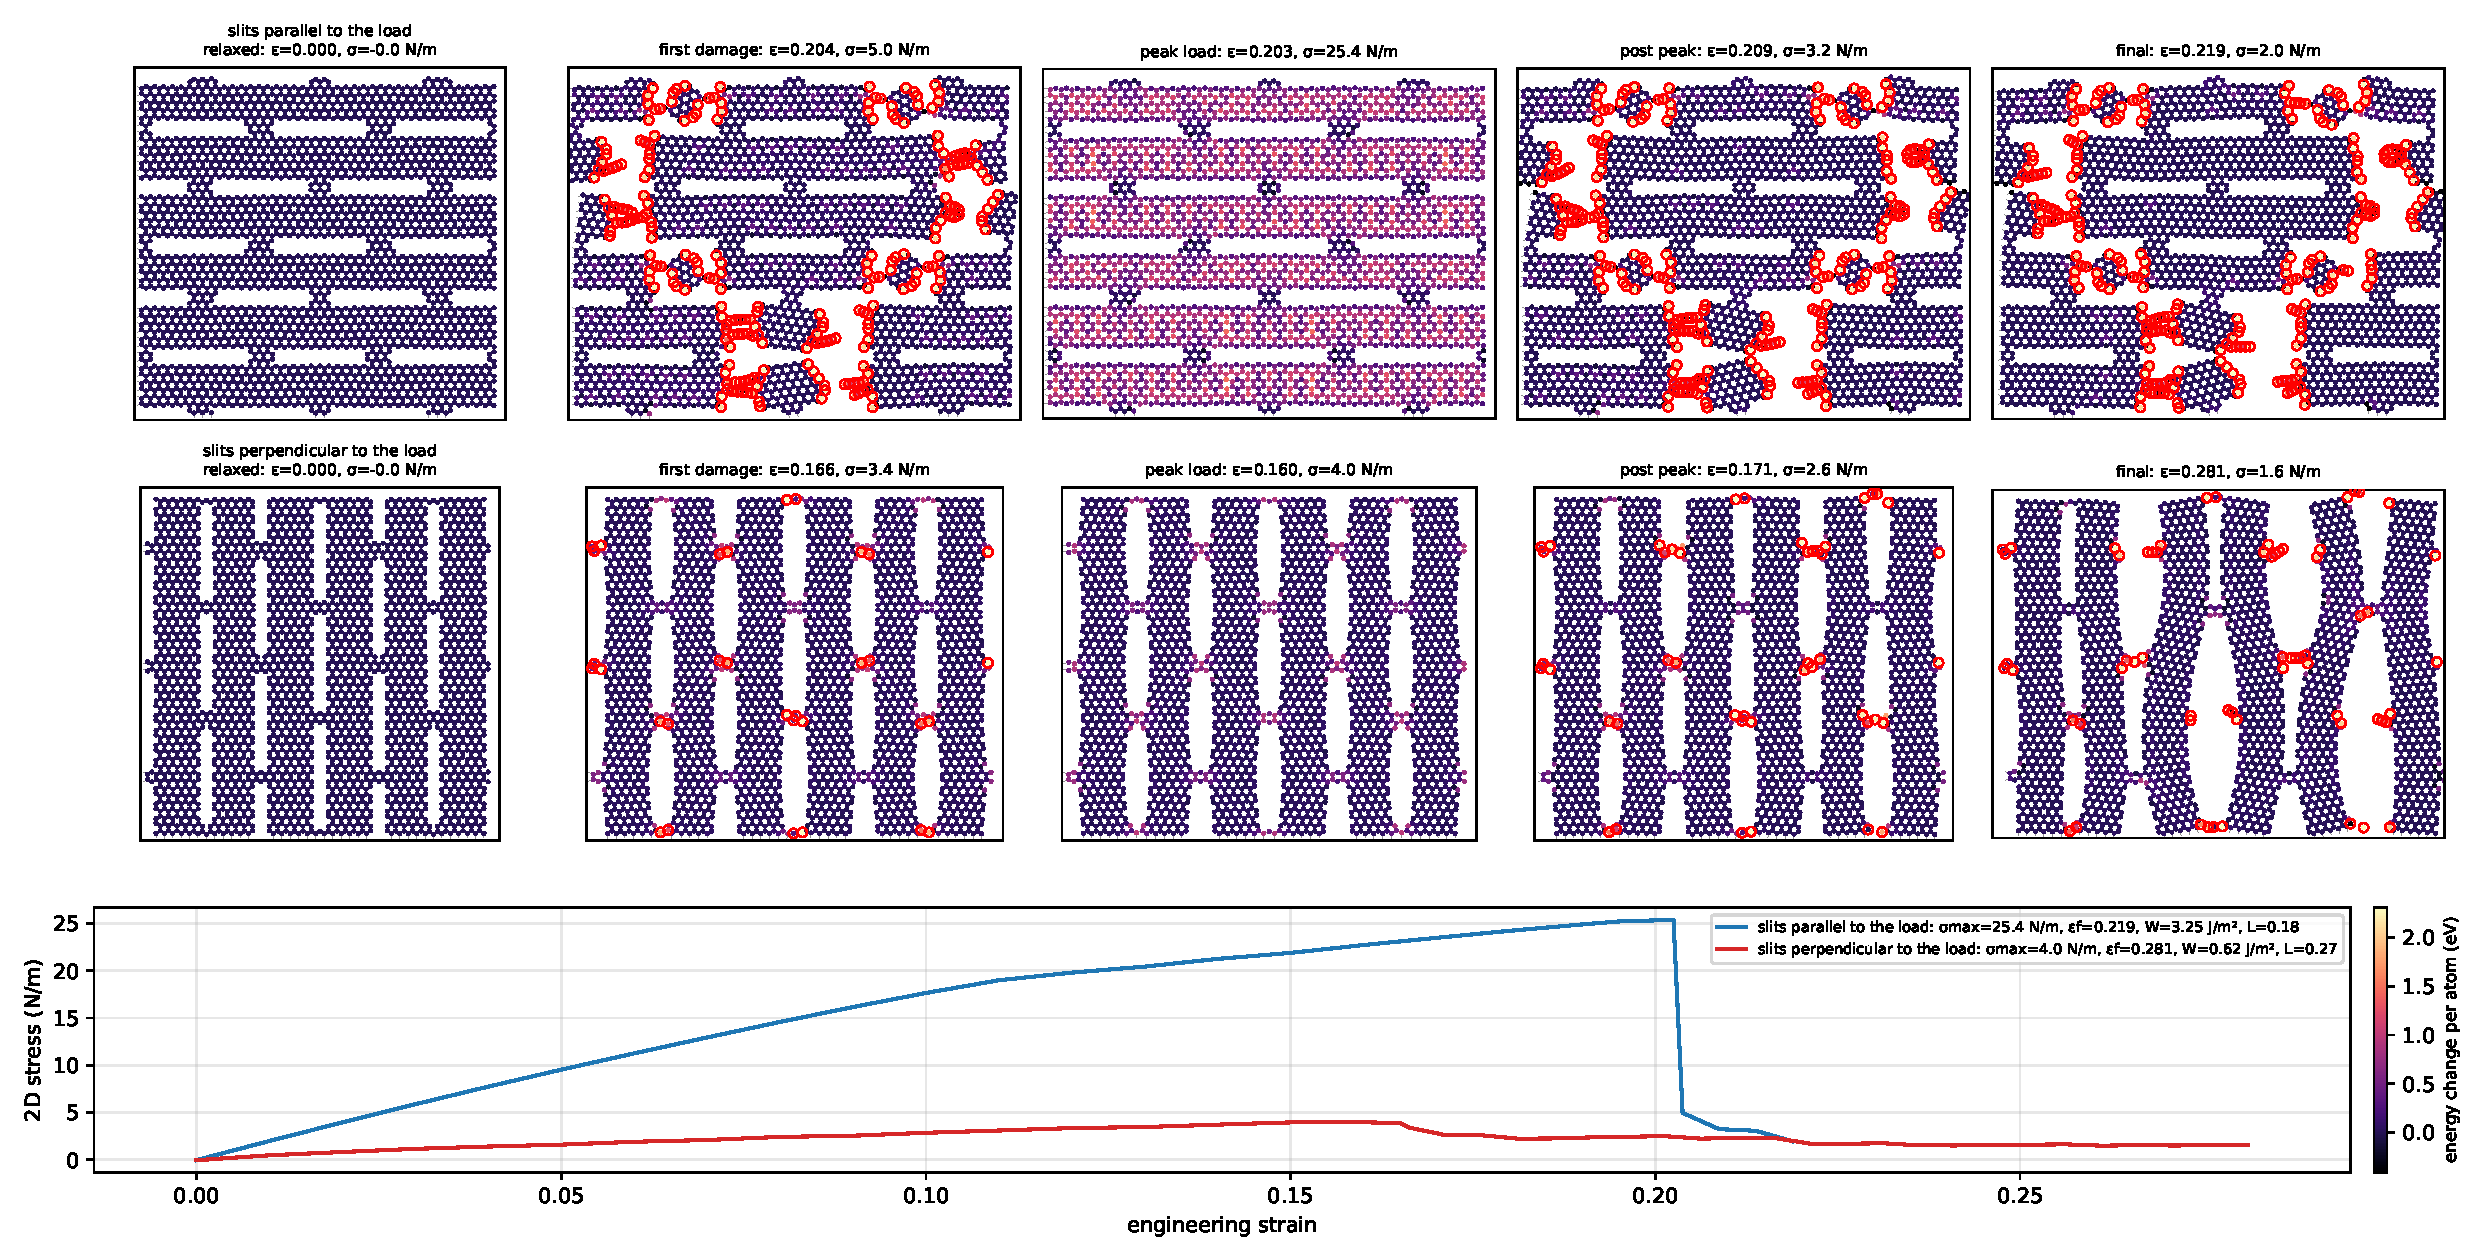
\includegraphics[width=1.0\textwidth]{progression/comparison_loadpath_orientation.pdf}\caption{Load-path organisation at identical porosity: slits parallel to the load (top, 25.4 N/m) leave straight continuous ligaments and fail at 22\% strain; slits perpendicular to the load (bottom, 4.0 N/m) leave only short bridges between slit tips and fail progressively from 17\% strain.}\label{fig:comparison_loadpath_orientation}\end{figure}
\begin{figure}[H]\centering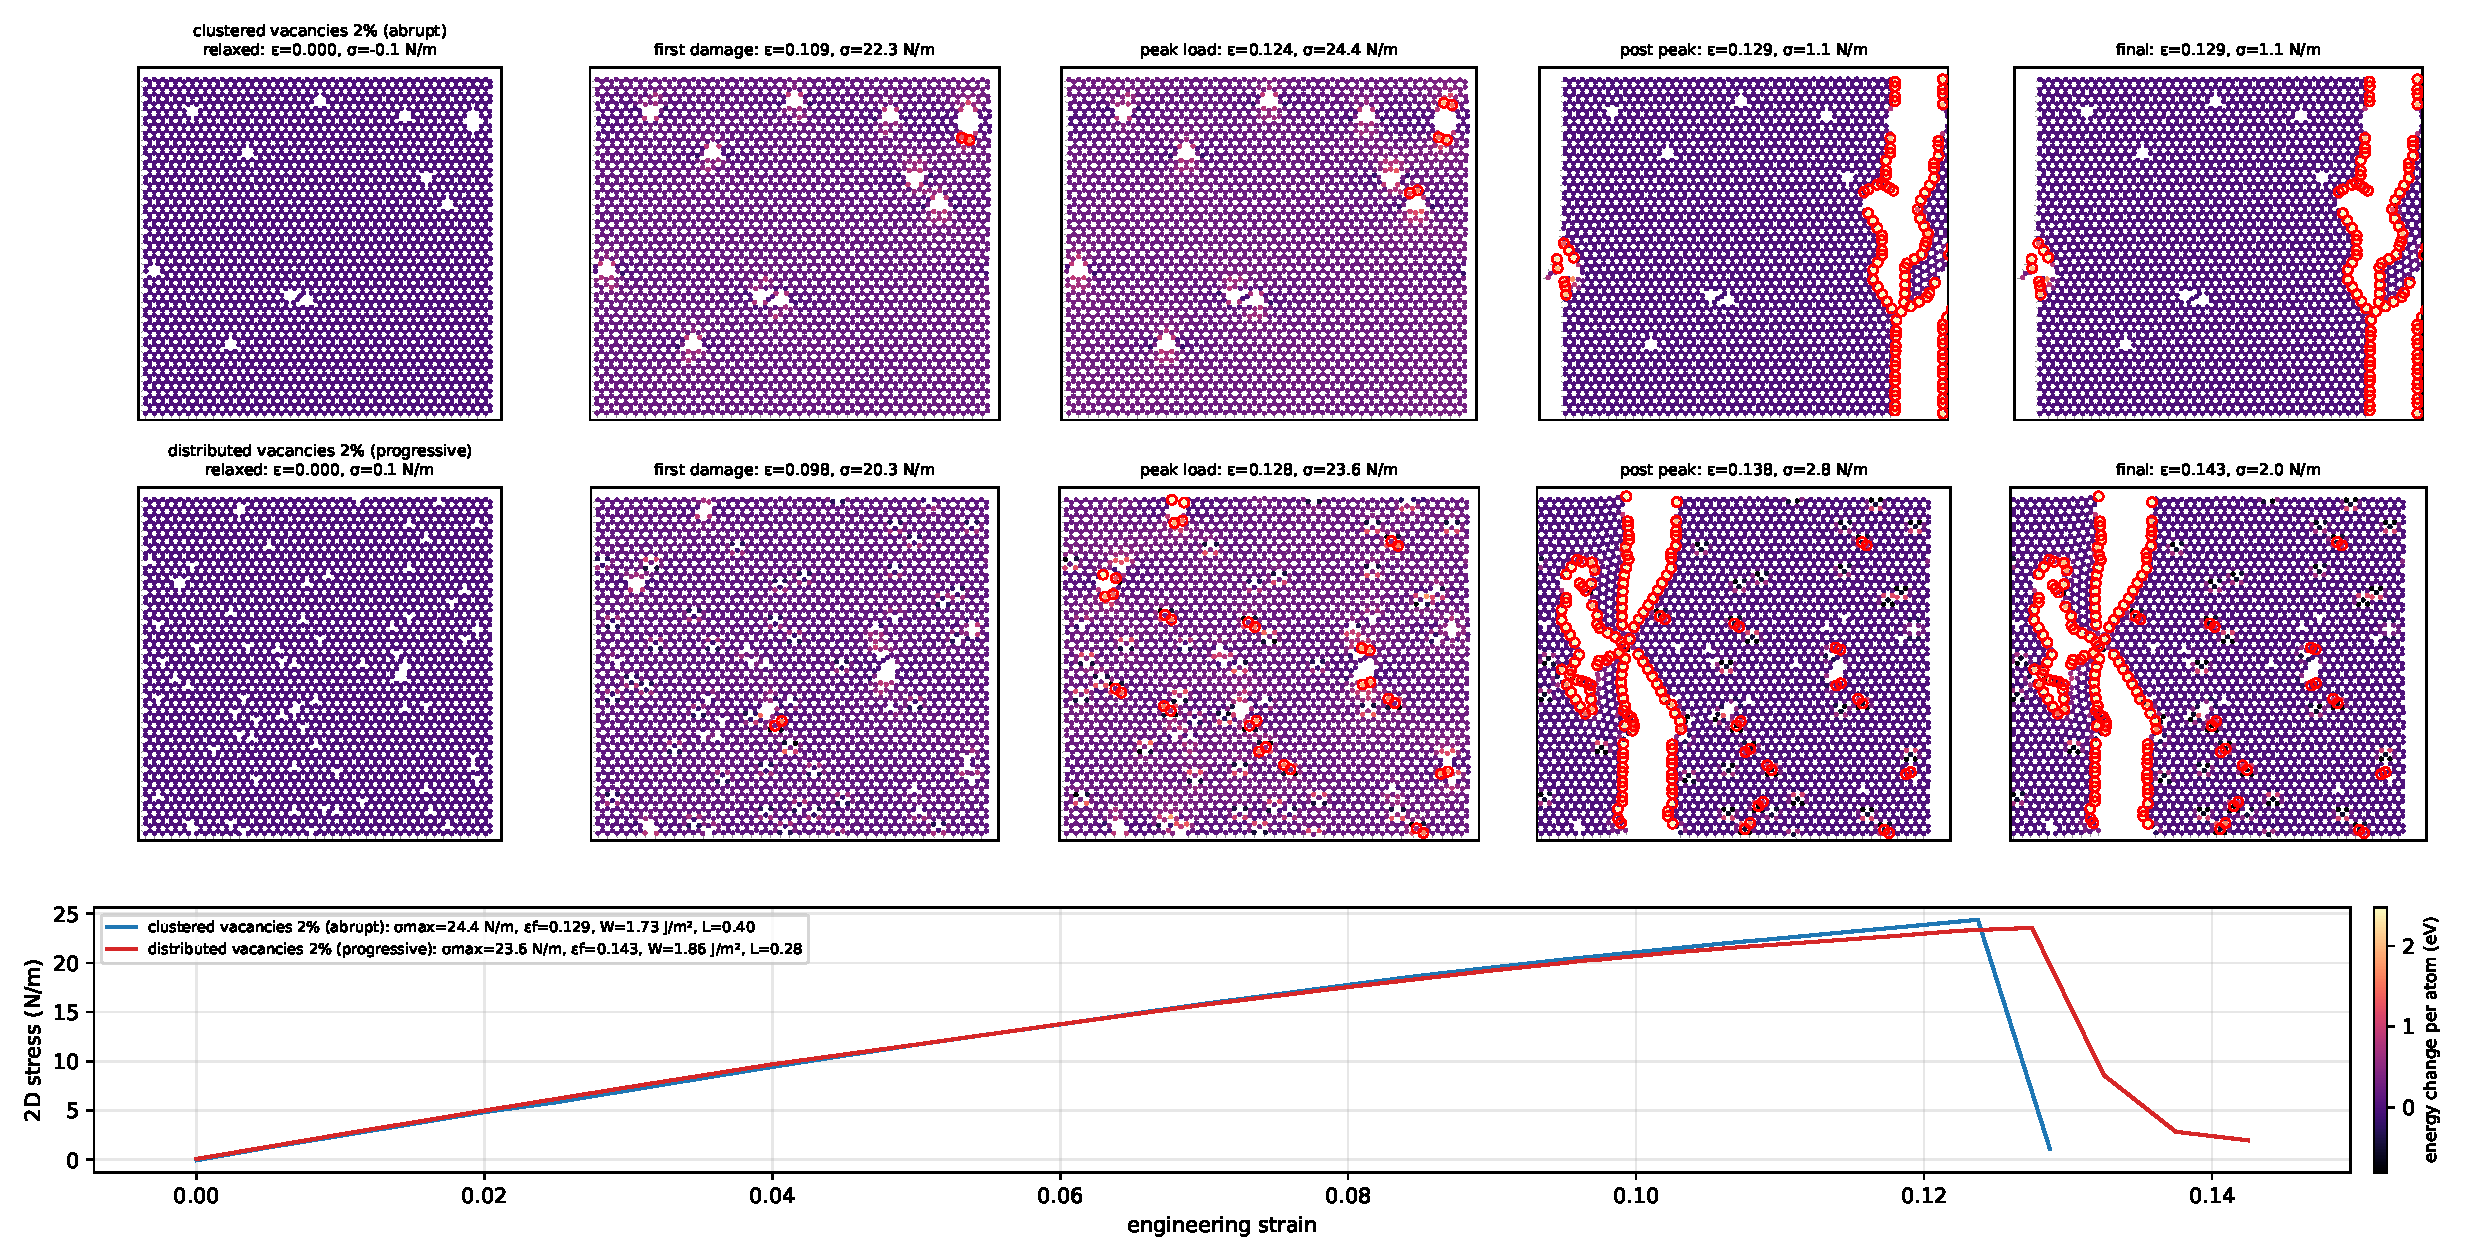
\includegraphics[width=1.0\textwidth]{progression/comparison_localised_vs_progressive.pdf}\caption{Localised versus progressive fracture at equal defect density and nearly equal strength: clustered vacancies (top, 24.4 N/m) fail in a single avalanche from one cluster, distributed vacancies (bottom, 23.6 N/m) lose bonds at several vacancies before the peak and retain load after it. Frames: relaxed, first bond loss, peak load, post-peak, final; colour = energy change per atom; red circles = atoms that lost a bond.}\label{fig:comparison_localised_vs_progressive}\end{figure}
\begin{figure}[H]\centering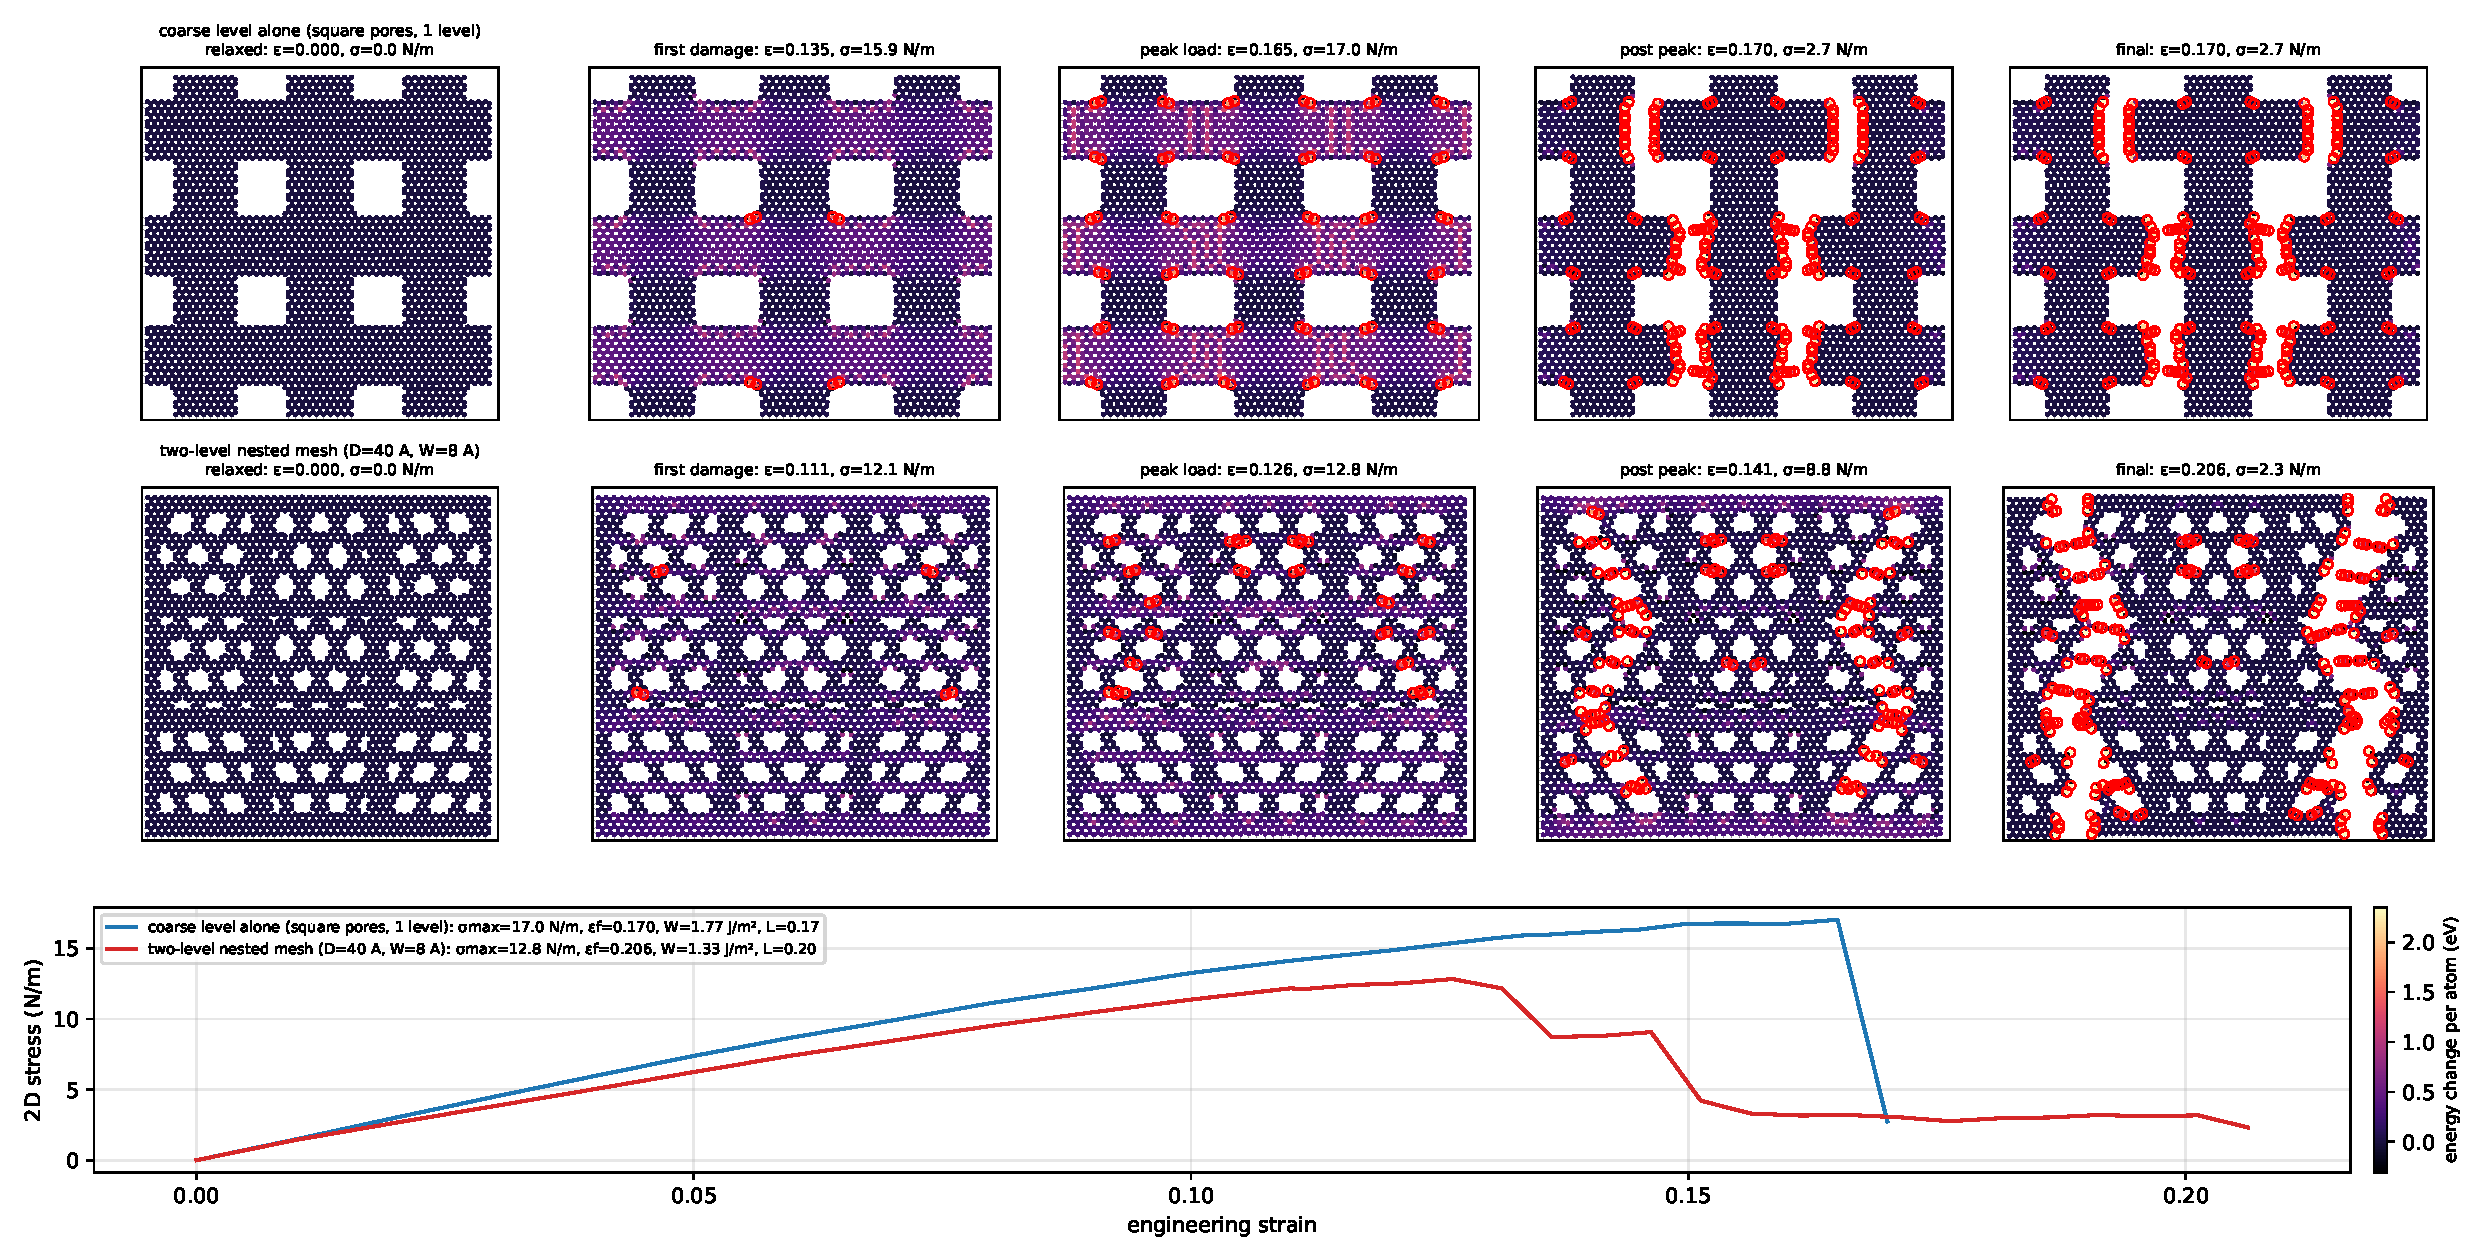
\includegraphics[width=1.0\textwidth]{progression/comparison_nonhierarchical_vs_hierarchical.pdf}\caption{Non-hierarchical versus hierarchical architecture at matched porosity 0.20 and footprint: the coarse square mesh (top, 17.0 N/m) accumulates harmless corner damage and then snaps all load-parallel ligaments together; the two-level nested mesh (bottom, 12.8 N/m) loses its fine level first, retains load on the load-parallel veins and fails through crack bands channelling along columns next to the load-perpendicular veins.}\label{fig:comparison_nonhierarchical_vs_hierarchical}\end{figure}
\begin{figure}[H]\centering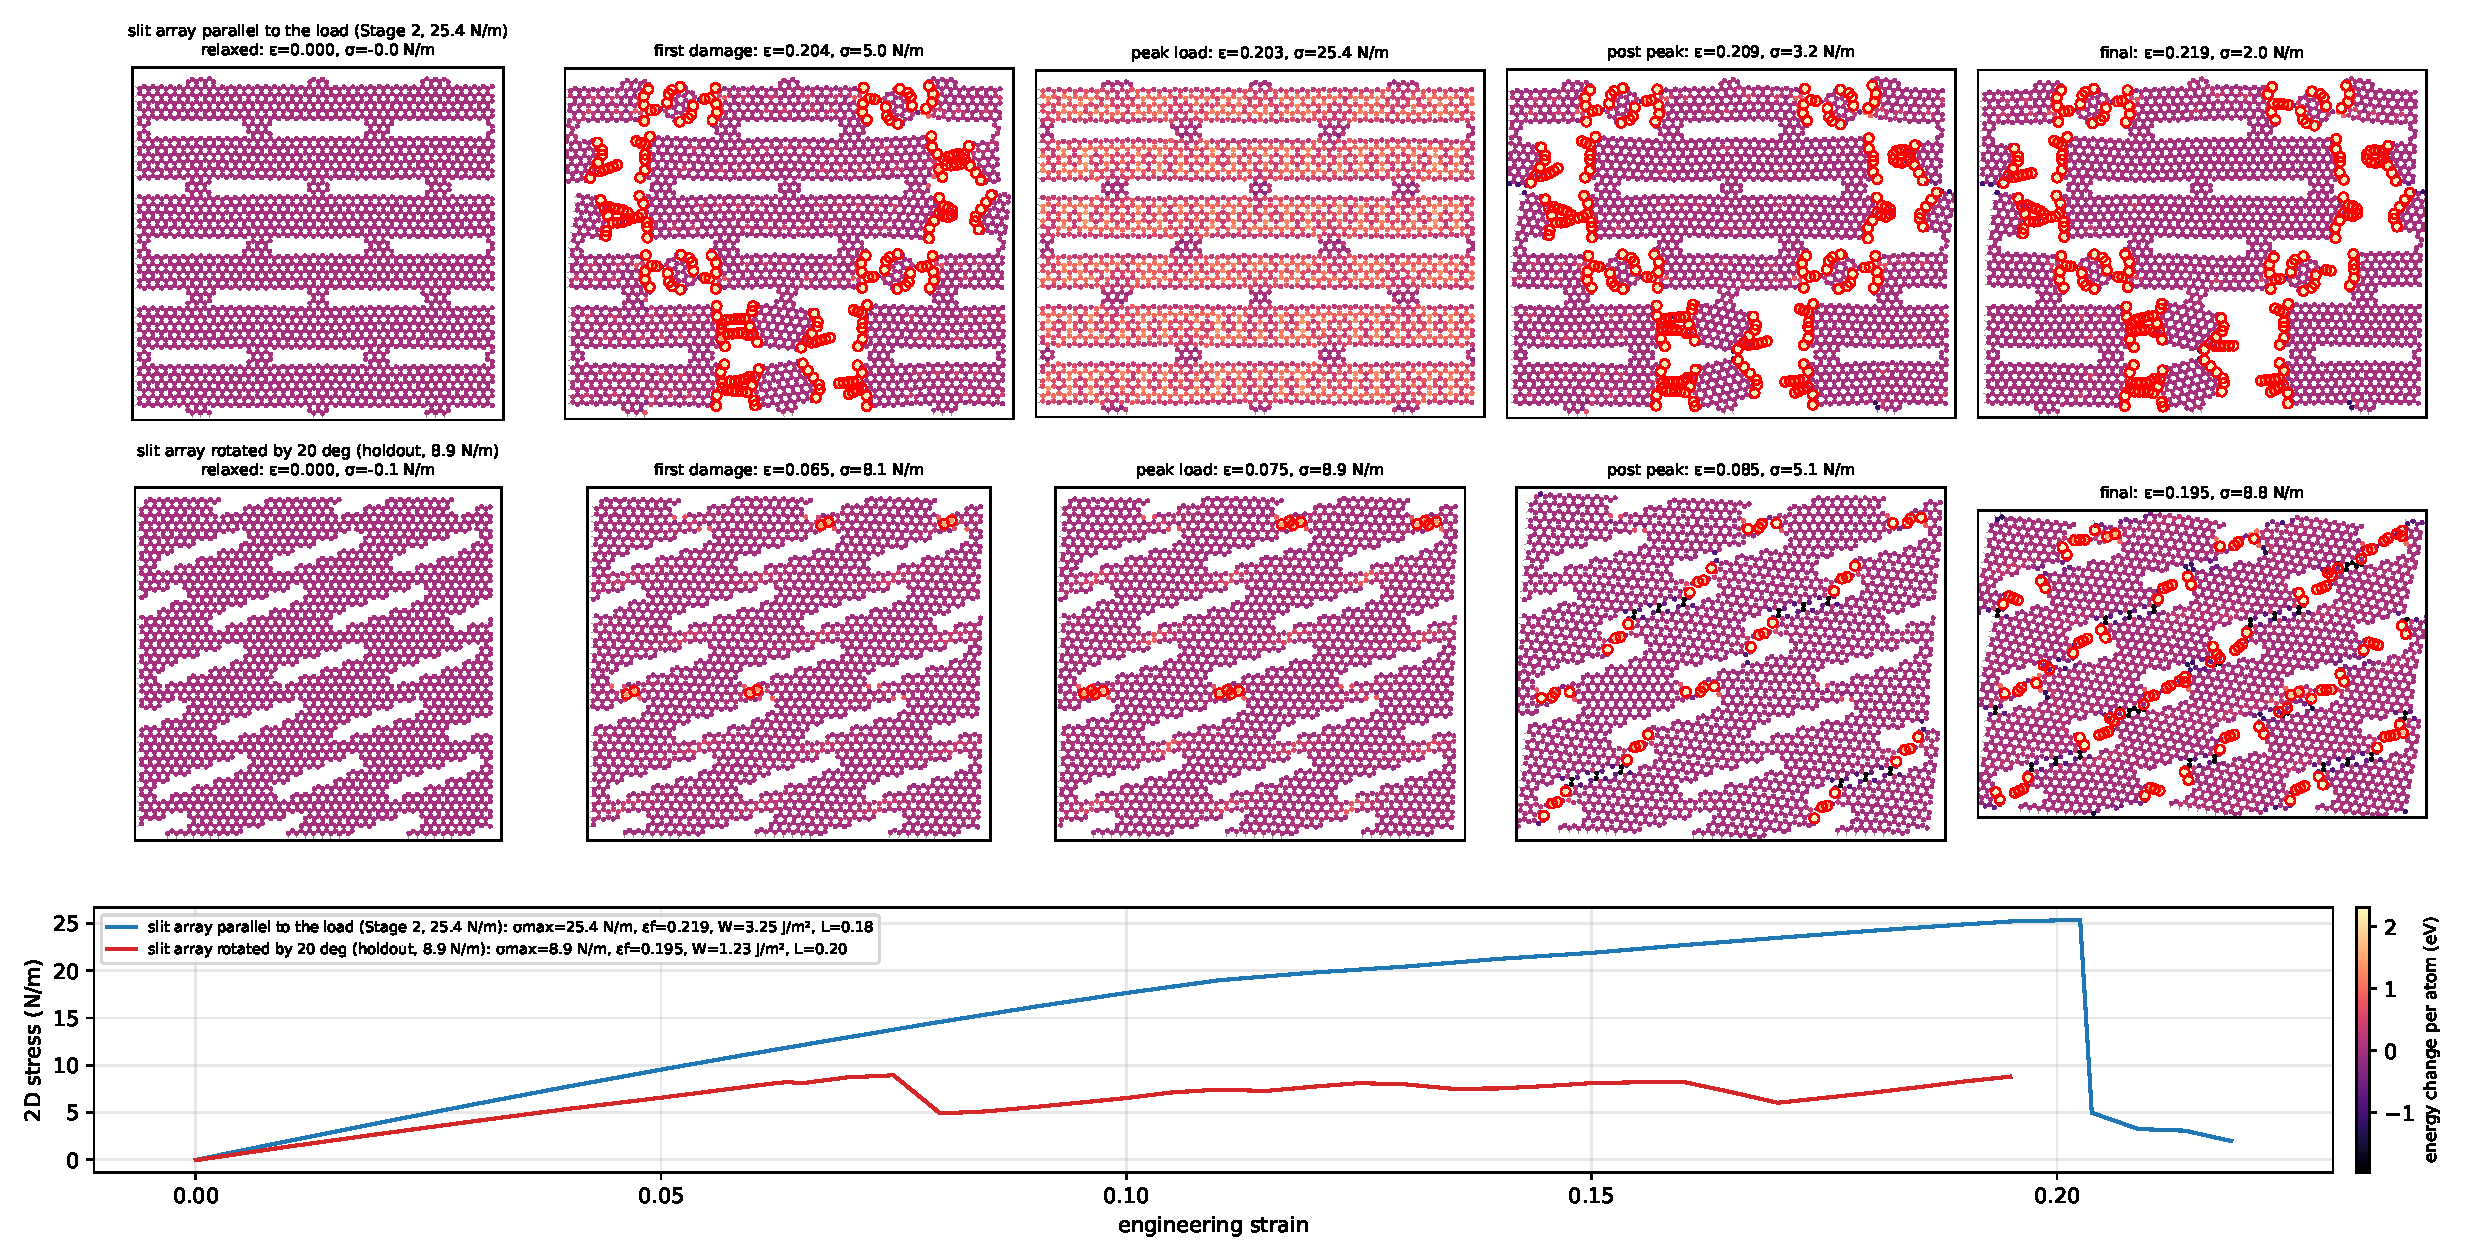
\includegraphics[width=1.0\textwidth]{progression/comparison_slit_orientation_echelon.pdf}\caption{Holdout: rotating a parallel slit array by 20 degrees reduces the strength from 25.4 to 8.9 N/m (predicted 23.9 N/m): the slit tips of neighbouring rows now overlap along the load and the ligaments between them fail by en-echelon crack coalescence, a mechanism absent from the training set. Rows: relaxed, first damage, peak load, post-peak, final; colour: energy change per atom; bottom: stress-strain curves with the selected events marked.}\label{fig:comparison_slit_orientation_echelon}\end{figure}


\section{Major mechanisms}
\label{sec:mech}
The campaign supports four mechanisms, each backed by matched comparisons and, where stochastic, by seed replicates.

\paragraph{1. Net section times ligament-size-dependent net-section strength.} The strength of a porous sheet is the minimum load-bearing solid fraction across the loading direction multiplied by a net-section strength that depends on the width and alignment of the load-bearing ligaments but not on pore shape: $\approx$30--32\,N/m (80\% of the intrinsic strength) for straight, load-parallel ligaments wider than $\sim$20\,\AA, 17--19\,N/m for round-pore ligaments of 10--13\,\AA, and 12--20\,N/m for random networks. Evidence: porosity independence of the parallel-slit strength, the linear net-section scaling of the square coarse mesh, the equality of square and round coarse pores at equal net section, the master plot of net-section strength versus ligament width, and the holdout predictions (Sec.~\ref{sec:holdout}). Mechanistically, the fine ligaments are weaker because a larger fraction of their bonds is perturbed by the two-coordinated pore edges (edge reconstruction and bond-order changes), an atomic-scale effect that has no continuum analogue at fixed geometry ratio.

\paragraph{2. Load-path orientation.} Ligaments or pores aligned with the load carry the stress without concentration; features across the load reduce the net section and concentrate stress at their ends. The same porosity yields 25.4 vs 4.0\,N/m for slits parallel vs perpendicular to the load, 19.0 vs 8.6\,N/m for ellipses, and 16.1 vs 12.0\,N/m for veins along vs across the load in nested meshes. This is the largest single lever in the design space and acts identically in single-scale and hierarchical structures.

\paragraph{3. Fibre-bundle load transfer sets the fracture mode.} After the first local failure, the released load is shared by the remaining parallel ligaments; failure is progressive only when the share transferred to each survivor stays below its strength margin, i.e. when there are many parallel paths of moderate strength dispersion. Few wide strips (three per cell) cascade even with 15\% dispersion (Stage~4), single flaws and clustered defects run in one event, whereas 8--10 rows of fine ligaments, jittered lattices, distributed vacancies and load-parallel-vein meshes fail row by row and retain 20--60\% of the peak load. Spatial localisation of the damage is a separate property: periodic single-avalanche failures are spatially delocalised, crack-like failures localised.

\paragraph{4. Lattice trapping of cracks.} Beyond $\approx$20\,\AA{} the strength of a cracked or holed sheet becomes independent of flaw size (18--19.5\,N/m for 20--50\,\AA{} flaws in 100--150\,\AA{} cells), because crack advance in the discrete lattice proceeds by trapped bond-breaking events with a barrier; stable bond-by-bond growth precedes the instability. Griffith scaling from the 10 and 20\,\AA{} cracks would have predicted 12--14\,N/m for the 40 and 50\,\AA{} cracks.

\paragraph{What hierarchy does.} A nested mesh behaves as the parallel combination of its finest level (which fails first) and its load-parallel coarse ligaments; at matched porosity it is never stronger than the coarse level alone, and never tougher than the fine level alone, unless the fine level is itself aligned with the load. Scale ratio, hierarchy depth and perpendicular veins are irrelevant or detrimental. Hierarchy is therefore not a mechanism in this model; alignment and ligament width are.

\section{Rejected hypotheses and counter-examples}
\begin{itemize}
\item \textbf{H-A (pore-shape knockdown) -- rejected in its original form.} Circular and square coarse pores at equal net section are equally strong (16.1 vs 17.0\,N/m; predicted 11.3). The net-section factor survived, the shape factor did not.
\item \textbf{H-C (load-path equivalence controls the mode) -- rejected.} Dispersing ligament widths by 15\% lowered strength in both coarse meshes and left the single-avalanche mode unchanged (square) or shortened the tail (round). Replaced by the fibre-bundle load-transfer criterion.
\item \textbf{H-D (disorder optimum for energy absorption) -- not supported after replication.} The Voronoi ``optimum'' at 60\% regularity was a single-seed outlier (14.4 vs 9.2/9.9\,N/m); jittered meshes lose strength without a reproducible gain in work ($1.07\pm0.31$ vs $1.16\pm0.30$\,J/m$^2$ for the ordered lattice across registries).
\item \textbf{H-F$'$ (veins as crack arrestors) -- rejected.} Load-perpendicular veins neither arrest cracks nor add strength (12.0\,N/m, equal to the fine mesh); cracks channel along the columns next to them.
\item \textbf{Flaw halo (P11) -- no shielding.} Pore rings around a hole cost strength relative to the bare hole (16.2 vs 19.1\,N/m); they only reduce the penalty relative to uniformly distributed porosity.
\item \textbf{Gradients (P10) -- detrimental.} Pore-size gradients along or radial to the load are weaker than the uniform mesh (10.1/10.0 vs 11.7\,N/m) because the largest pores define the weakest section.
\item \textbf{Node connectivity (P9) -- minor.} Six-connected triangulated struts are not stronger than four-connected ones; a continuous strut family along the load is what matters (11.5 vs 7.4 vs 6.0\,N/m).
\item \textbf{Unstable and strongly reconstructed candidates.} Every generated geometry relaxed to a mechanically continuous structure, but 6\,\AA{} struts, 20\,\AA{}-vein meshes with residual 2-atom pores, and the 0.40-porosity mesh reconstructed by more than 1\,\AA{} (flagged ``strongly reconstructed''); their results are reported with that flag. No structure fragmented, and none is claimed to be synthesizable.
\item \textbf{Counter-examples worth keeping.} The 45$^\circ$ slit lattice sheds load at 17\% strain and then re-stiffens to $>15$\,N/m at 30\% by ligament rotation (geometric compliance); the 30\,\AA{} crack is not weaker than the 20\,\AA{} crack; the fine period-12 mesh is stronger than the period-16 mesh at equal porosity, but the difference (13.3 vs 11.7\,N/m) is within the $\approx$12\% registry effect measured in Stage~6.
\end{itemize}

\section{Limitations}
\begin{itemize}
\item \textbf{Model, not experiment.} Every number in this report is a property of the screened second-generation REBO potential under athermal quasi-static loading. \rebo{} underestimates the in-plane stiffness of graphene by $\sim$30\% and overestimates its Poisson ratio; intrinsic strengths and the qualitative bond-breaking chemistry are reasonable, but absolute strengths and failure strains should be read as model quantities. No structure is claimed to be synthesizable; generated structures are not new allotropes.
\item \textbf{Athermal, quasi-static, 2D-planar.} Thermal activation, rate effects and out-of-plane deformation (buckling, wrinkling of ligaments) are absent by construction; the sheets are kept planar. The optional MD module allows finite-temperature checks but was not used for the main campaign.
\item \textbf{Periodic supercells.} Loading is applied to periodic cells of 100--120\,\AA; pores and cracks interact with their periodic images, and the coarsest hierarchical level is limited by the cell. Size effects were checked (TEST~15) but not eliminated.
\item \textbf{Uniaxial-stress protocol.} The transverse cell is relaxed to $\sigma_{yy}=0$ by a secant scheme with a trust region; for strongly non-monotonic transverse responses (pristine zigzag graphene above 16\% strain) the followed branch depends on history.
\item \textbf{Bond definition.} Damage is inferred from a geometric criterion ($r<2.0$\,\AA) applied to converged states; events shorter than one strain increment are invisible, and the bisection resolves only the first event to 0.125\%.
\item \textbf{Float32 fast mode.} The campaign used float32 on the Apple GPU; differences to the float64 reference are $10^{-4}$\,eV/\AA{} in forces and $10^{-5}$\,N/m in stress, but MPS reductions are order-non-deterministic at the $10^{-7}$ level, so post-instability branches of a given run are reproducible only statistically (Stage~6 seeds address the structural, not the numerical, variability).
\item \textbf{Descriptors.} Structural descriptors are raster/graph based and coarse (0.5\,\AA{} raster, 8$\times$8 localisation grid); the automatic fracture-mode classification uses fixed thresholds.
\item \textbf{Sampling.} About one hundred simulations cannot cover a twelve-dimensional design space densely; the study identifies mechanisms and regimes, not optima.
\end{itemize}

\section{Threats to validity}
\begin{itemize}
\item \textbf{Circularity.} Hypotheses were formed from Stage~1--2 data and tested on new structures in Stage~4 and on holdouts in Stage~7--8; the prediction files are timestamped and hashed before the corresponding simulations were launched. Retrospective modification of predictions was not performed.
\item \textbf{Confounding.} Comparisons across architectures are controlled for porosity (mass per footprint) and cell size, but not simultaneously for every descriptor (edge-atom fraction, ligament width and net section co-vary with the architecture); the property maps and matched pairs in Stage~4 separate these where possible.
\item \textbf{Numerical artefacts.} Non-converged minimisations are flagged in every record; the effect of tolerance, strain increment and cell size was quantified (TESTS~13--15). Screening switch-on features and the affine cut-off re-stiffening are documented and do not affect relaxed trajectories.
\item \textbf{Selection of top structures.} The showcase set was chosen by predefined categories (reference, strongest, most work, Pareto member, hierarchical, most localised, most progressive, flaw halo, counter-example), not by visual appeal.
\item \textbf{Stochastic variability.} Disordered structures were replicated with $\ge3$ seeds in Stage~6; conclusions about disorder rely on those distributions, individual seeds are reported.
\end{itemize}

\section{Conclusions}
A validated, GPU-resident implementation of screened REBO2 was used to run an autonomous, hypothesis-driven study of how atomic-scale architecture controls the fracture of graphene-derived sheets, with the reference images serving as a source of design principles rather than templates. The findings, all statements about the \rebo{} model under athermal quasi-static uniaxial tension, are:
\begin{enumerate}
\item Strength is governed by the minimum load-bearing solid fraction across the load multiplied by a net-section strength that depends on ligament width and alignment (30--32\,N/m for straight, load-parallel ligaments wider than $\sim$20\,\AA; 17--19\,N/m for 10--13\,\AA{} round-pore ligaments; 12--20\,N/m for random networks), not on pore shape, porosity per se, hierarchy depth or scale ratio.
\item Load-path orientation is the largest lever: identical porosity yields 25 vs 4\,N/m for slits parallel vs perpendicular to the load, and 16 vs 12\,N/m for coarse veins along vs across the load.
\item Hierarchy adds no strength or toughness at matched mass unless its levels are aligned with the load; the only nested designs that beat the coarse-only limit combine load-elongated fine pores with veins (17.5\,N/m with square veins, progressive; 19.4\,N/m with load-parallel veins, stepwise; both 2.0\,J/m$^2$).
\item The fracture mode is a load-transfer (fibre-bundle) property: many parallel ligaments of moderate dispersion fail progressively and retain load, few equivalent wide strips, clustered defects and single flaws fail in one avalanche; strength dispersion alone does not create progressivity.
\item Cracks and holes larger than $\approx$20\,\AA{} sit on a lattice-trapping plateau (18--19.5\,N/m for 20--50\,\AA{} flaws), far above Griffith scaling.
\item Disorder, gradients and flaw halos are costs, not toughening mechanisms, in this model; apparent optima disappeared under seed replication, and the atomic registry of pore edges alone shifts fine-mesh strength by $\approx$12\%.
\item Twelve holdout designs predicted before simulation gave a median strength error of 14\% and the correct single-avalanche/multi-event classification in 10 of 12 cases; the misses identified a chirality-dependent ligament strength, the additivity of alignment effects across scales (best nested design 19.4\,N/m), the weakest-section rule for halos and gradients, and a new mechanism, en-echelon slit coalescence, at which load-path alignment is lost (8.9 instead of the predicted 23.9\,N/m).
\end{enumerate}
The platform, database (\nRuns{} records), structures, trajectories, figures, movies and this report are delivered as one reproducible archive; every simulation can be regenerated from its record.

\section{Damage and connectivity analysis}
\label{sec:damage}
Two carbon atoms are counted as bonded when their distance is below 2.0\,\AA{} (between the equilibrium bond length of 1.42\,\AA{} and the inner cut-off region 1.95--2.25\,\AA{} of \rebo{}; bonds at the tensile instability are 1.7--1.8\,\AA{} long and ruptured pairs relax to more than 2.5\,\AA{} within one increment). Bond sets are compared between consecutive converged states; every lost bond is recorded with the strain, the two atoms and the midpoint of the bond. Persistence is enforced in post-processing (a bond that reappears is not counted as damage). The damage-localisation measure is $L=1-H/H_\mathrm{max}$, where $H=-\sum_i p_i\ln p_i$ is the Shannon entropy of the distribution $p_i$ of damage-event midpoints over an $8\times8$ grid of the periodic cell and $H_\mathrm{max}=\ln 64$; $L=0$ for uniformly distributed damage and $L=1$ if all events fall in one cell. Load-bearing connectivity is tested by percolation of the bond graph across the periodic $x$ boundary (a doubled-cell union-find). Fracture modes are classified automatically from the number of discrete damage steps, the fraction of bonds lost in the largest single step, the post-peak strain range and the post-peak load retention (\texttt{analysis/metrics.py}).



\appendix
\section{Validation table}
\begingroup\footnotesize\setlength{\tabcolsep}{4pt}
\begin{longtable}{>{\raggedright\arraybackslash}p{1.1cm}>{\raggedright\arraybackslash}p{4.4cm}>{\raggedright\arraybackslash}p{2.7cm}>{\raggedright\arraybackslash}p{4.1cm}>{\raggedright\arraybackslash}p{1.2cm}p{0.9cm}}
\caption{Validation suite: expected result, observed result, numerical error, tolerance and status (PASS/FAIL). Details in \texttt{validation/results/}.}\label{tab:validation}\\
\toprule test & name & expected & observed & error & status\\ \midrule\endfirsthead
\toprule test & name & expected & observed & error & status\\ \midrule\endhead
TEST 1 & energy vs Atomistica Rebo2Scr (cpu f64), 12 configurations incl. pore edges, crack tips, near rupture & identical & max $|$dE$|$/atom = 6.11e-14 eV & 6.1e-14 (tol 1e-09) & \textbf{PASS}\\
TEST 2 & forces vs Atomistica (every component), same configurations & identical & max $|$dF$|$ = 4.26e-13 eV/A & 4.3e-13 (tol 1e-08) & \textbf{PASS}\\
TEST 3 & finite-difference forces (central, h=1e-4 A) and stress (h=1e-5) & F = -dE/dR & max $|$F - F\_fd$|$ = 4.8e-06 eV/A ($|$F$|$ up to 31) & 4.8e-06 (tol 1e-04) & \textbf{PASS}\\
TEST 9 & cell-list neighbour list vs brute-force enumeration (pair sets) & identical pair sets & identical & 0.0e+00 (tol 0e+00) & \textbf{PASS}\\
TEST 10 & translation invariance (rigid shift 7.3,-11.1 A) & dE = 0 & dE = 0.0e+00 eV, max dF = 4.9e-13 & 4.9e-13 (tol 1e-09) & \textbf{PASS}\\
TEST 11 & total force balance sum\_i F\_i & 0 & 1.1e-14 eV/A & 1.1e-14 (tol 1e-10) & \textbf{PASS}\\
TEST 12 & periodic-image invariance (wrapping, 2x supercell) & invariant & max deviation 1.1e-12 & 1.1e-12 (tol 1e-09) & \textbf{PASS}\\
TEST 4 & fast mode (mps float32) vs reference (cpu float64): energies/forces/stress on relaxed structures & agreement within float32 round-off & $|$dE$|$/atom $<$= 6.7e-06 eV, $|$dF$|$ $<$= 1.5e-04 eV/A, $|$dsigma$|$ $<$= 4.0e-05 N/m & 1.5e-04 (tol 5e-03) & \textbf{PASS}\\
TEST 16 & precision near fracture (pre-damage, peak, post-peak frames), mps f32 vs cpu f64 & within float32 round-off & $|$dF$|$ $<$= 1.5e-04 eV/A, $|$dsigma$|$ $<$= 4.0e-05 N/m & 1.5e-04 (tol 5e-03) & \textbf{PASS}\\
TEST 17 & reproducibility of repeated evaluations (fast device) & identical up to reduction-order round-off & dE = 4.9e-04 eV total, max dF = 1.2e-07 eV/A & 1.2e-07 (tol 1e-05) & \textbf{PASS}\\
TEST 5 & relaxed lattice constant / bond length (cpu f64 vs Atomistica; fast mode) & a0 = 2.460177 A (bond 1.420384) & a0 = 2.460177 A (f64), 2.460591 A (f32) & 6.1e-09 (tol 1e-06) & \textbf{PASS}\\
TEST 6 & graphene cohesive energy & -7.395110 eV/atom & -7.395110 eV/atom & 5.3e-15 (tol 1e-08) & \textbf{PASS}\\
TEST 7 & small-strain elastic response (C11, C12, Y2D, nu) relaxed & Y2D = 245.07 N/m, nu = 0.3919 (Atomistica) & Y2D = 245.07 N/m, nu = 0.3919 & 2.3e-10 (tol 1e-03) & \textbf{PASS}\\
TEST 8 & armchair vs zigzag tensile response (homogeneous, relaxed, to 30\% strain) & zz peak 37.73 N/m, ac peak 30.48 N/m & zz 37.73, ac 30.48 N/m; max $|$dsigma$|$ = 2.3e-13 & 2.3e-13 (tol 1e-03) & \textbf{PASS}\\
TEST 13 & minimiser convergence (fmax 0.05 -$>$ 0.005 eV/A, 64 A nanomesh) & metrics converge; production fmax=0.02 within 3\% of fmax=0.005 & fmax=0.05: sigma=11.43 N/m, eps\_fd=0.1413, eps\_f=0.3413, FIRE its=-1; fmax=0.02: sigma=11.41 N/m, eps\_fd=0.1388, eps\_f=0.2088, FIRE its=-1; fmax=0.01: sigma=11.35 N/m, eps\_fd=0.1375, eps\_f=0.1775, FIRE its=-1; fmax=0.005: sigma=11.35 N/m, eps\_fd=0.1375, eps\_f=0.1725, FIRE its=123710 & 9.1e-03 (tol 3e-02) & \textbf{PASS}\\
TEST 14 & strain-increment convergence (1\%, 0.5\%, 0.25\% with bisection; 0.5\% without) & production increment 0.5\% (+bisection) within 3\% of 0.25\% for strength and first-damage strain & d\_eps=0.01: sigma=11.41 N/m, eps\_fd=0.1387, eps\_f=0.2188, W=1.30; d\_eps=0.005: sigma=11.41 N/m, eps\_fd=0.1388, eps\_f=0.2088, W=1.18; d\_eps=0.0025: sigma=11.41 N/m, eps\_fd=0.1388, eps\_f=0.1938, W=1.24; d\_eps=0.005 no refinement: sigma=11.33 N/m, eps\_fd=0.1400, eps\_f=0.1850, W=1.14 & 9.1e-05 (tol 3e-02) & \textbf{PASS}\\
TEST 15 & system-size convergence (exact periodic repeats of a 32 A mesh pattern: 1x, 2x, 3x; fixed 12 A crack in 40/60/90 A cells) & strength of periodic repeats size-independent within 5\%; crack strength converges with cell size (image interaction) & mesh repeats: L=32: sigma=16.08, eps\_fd=0.1350, eps\_f=0.1750; L=64: sigma=16.07, eps\_fd=0.1350, eps\_f=0.2500; L=96: sigma=16.01, eps\_fd=0.1338, eps\_f=0.2538 $|$ crack 12 A: cell 40: sigma=22.02, eps\_fd=0.1163; cell 60: sigma=21.21, eps\_fd=0.1000; cell 90: sigma=21.86, eps\_fd=0.0963 & 4.5e-03 (tol 5e-02) & \textbf{PASS}\\
TEST 18 & complete stress-strain curve: Torch engine vs Atomistica backend in an AQS (same protocol: 1\% steps, fixed transverse, FIRE fmax 0.02), precrack + nanomesh & identical curves with the same minimiser; batched driver within the fmax-induced stress uncertainty (~0.2 N/m) & Torch+ASE FIRE vs Atomistica+ASE FIRE: max $|$dsigma$|$ = 2.0e-10 N/m (identical incl. fracture); batched FIRE driver: 0.09 N/m (cpu f64), 0.07 N/m (mps f32) up to the peak & 9.1e-02 (tol 2e-01) & \textbf{PASS}\\
TEST 19 & bond separation E(r), F(r) through rupture (dimer, in-lattice bond, crack tip, homogeneous stretch) vs Atomistica & identical & max $|$dF$|$ = 1.2e-11 eV/A (cpu f64); fast f32 within 1.3e-02 & 1.2e-11 (tol 1e-08) & \textbf{PASS}\\
TEST 20 & export/data consistency (extxyz, xyz, traj, LAMMPS data, CIF, POSCAR round trip) & positions/cell preserved & extxyz: ok; xyz: ok; traj: ok; lammps-data: ok; cif: ok; vasp: ok & 4.3e-09 (tol 1e-03) & \textbf{PASS}\\
\bottomrule\end{longtable}\endgroup
\section{Experiment database}
\label{app:database}
The complete machine-readable database (one JSON record per run, stress--strain CSV files, structures and trajectories) is part of the deliverable (\texttt{experiments/database/}, \texttt{trajectories/}). Table~\ref{tab:database} lists every completed discovery simulation.
\begin{landscape}\footnotesize\setlength{\tabcolsep}{4pt}
\begin{longtable}{llllllllllllll}
\caption{Complete experiment database (discovery campaign): one row per simulation. $Y$ = 2D modulus (N/m), $\sigma$ = strength (N/m), $\varepsilon_p$ strain at peak, $\varepsilon_{fd}$ first-damage strain, $\varepsilon_f$ failure strain, $W$ work to failure (J/m$^2$), $L$ damage localisation.}\label{tab:database}\\
\toprule name & stage & N & phi & H & viability & Y & sigma & eps\_p & eps\_fd & eps\_f & W & L & mode\\ \midrule\endfirsthead
\toprule name & stage & N & phi & H & viability & Y & sigma & eps\_p & eps\_fd & eps\_f & W & L & mode\\ \midrule\endhead
S1\_hole\_d20 & S1 & 3648 & 0.033 & 1 & stable & 229.7 & 19.06 & 0.092 & 0.092 & 0.098 & 0.99 & 0.53 & abrupt\\
S1\_mesh\_p16\_phi0.2 & S1 & 2934 & 0.222 & 1 & reconstr. & 118.7 & 11.95 & 0.141 & 0.101 & 0.171 & 1.12 & 0.26 & progressive\\
S1\_precrack\_L10 & S1 & 3757 & 0.004 & 0 & stable & 245.3 & 24.08 & 0.114 & 0.114 & 0.119 & 1.55 & 0.47 & abrupt\\
S1\_precrack\_L20 & S1 & 3744 & 0.007 & 0 & stable & 235.1 & 18.53 & 0.086 & 0.081 & 0.091 & 0.89 & 0.52 & abrupt\\
S1\_precrack\_L30 & S1 & 3727 & 0.012 & 0 & stable & 223.7 & 18.72 & 0.099 & 0.079 & 0.104 & 1.05 & 0.44 & abrupt\\
S1\_pristine\_ac & S1 & 576 & 0.000 & -- & stable & 287.0 & 30.66 & 0.180 & 0.300 & 0.300 & 7.05 & 0.02 & abrupt\\
S1\_pristine\_zz & S1 & 576 & 0.000 & -- & stable & 250.1 & 38.79 & 0.270 & 0.271 & 0.271 & 6.73 & 0.31 & abrupt\\
S1\_vac\_clustered\_2pct & S1 & 3724 & 0.013 & 0 & reconstr. & 243.5 & 24.39 & 0.124 & 0.109 & 0.129 & 1.73 & 0.40 & abrupt\\
S1\_vac\_random\_2pct & S1 & 3691 & 0.021 & 0 & stable & 245.9 & 23.56 & 0.128 & 0.098 & 0.143 & 1.86 & 0.28 & progressive\\
S2\_H1\_p12 & S2 & 4398 & 0.199 & 1 & reconstr. & 123.5 & 13.26 & 0.146 & 0.121 & 0.221 & 1.45 & 0.25 & progressive\\
S2\_H1\_p16 & S2 & 4352 & 0.207 & 1 & reconstr. & 122.7 & 11.73 & 0.118 & 0.107 & 0.133 & 0.89 & 0.43 & progressive\\
S2\_H1\_p32 & S2 & 4376 & 0.203 & 1 & reconstr. & 145.8 & 16.44 & 0.164 & 0.134 & 0.264 & 1.94 & 0.12 & stepwise\\
S2\_H1\_square\_D40 & S2 & 4378 & 0.202 & 1 & stable & 150.5 & 17.02 & 0.165 & 0.135 & 0.170 & 1.77 & 0.17 & abrupt\\
S2\_H2\_D24\_W8 & S2 & 4425 & 0.194 & 2 & reconstr. & 149.3 & 14.34 & 0.137 & 0.122 & 0.158 & 1.31 & 0.24 & progressive\\
S2\_H2\_D40\_W12 & S2 & 4408 & 0.197 & 2 & reconstr. & 145.3 & 13.74 & 0.128 & 0.107 & 0.213 & 1.40 & 0.24 & progressive\\
S2\_H2\_D40\_W4 & S2 & 4368 & 0.204 & 2 & reconstr. & 131.3 & 13.22 & 0.141 & 0.126 & 0.261 & 1.50 & 0.23 & stepwise\\
S2\_H2\_D40\_W8 & S2 & 4377 & 0.202 & 2 & reconstr. & 132.3 & 12.83 & 0.126 & 0.111 & 0.206 & 1.33 & 0.20 & progressive\\
S2\_H2\_D60\_W8 & S2 & 4368 & 0.204 & 2 & reconstr. & 125.6 & 12.74 & 0.124 & 0.114 & 0.139 & 0.99 & 0.35 & progressive\\
S2\_H3\_D30\_120 & S2 & 4410 & 0.196 & 3 & reconstr. & 128.7 & 12.98 & 0.143 & 0.117 & 0.153 & 1.20 & 0.16 & progressive\\
S2\_ellipse\_0deg & S2 & 3008 & 0.203 & 1 & reconstr. & 87.7 & 8.61 & 0.141 & 0.136 & 0.236 & 1.07 & 0.24 & progressive\\
S2\_ellipse\_90deg & S2 & 3040 & 0.194 & 1 & reconstr. & 171.2 & 18.95 & 0.156 & 0.131 & 0.191 & 1.94 & 0.22 & progressive\\
S2\_graded\_radial & S2 & 3080 & 0.183 & 1 & reconstr. & 134.9 & 9.97 & 0.083 & 0.084 & 0.199 & 0.76 & 0.39 & progressive\\
S2\_graded\_x & S2 & 3002 & 0.204 & 1 & reconstr. & 131.3 & 10.09 & 0.090 & 0.091 & 0.096 & 0.51 & 0.50 & abrupt\\
S2\_hole20\_background & S2 & 3379 & 0.104 & 1 & reconstr. & 171.1 & 13.21 & 0.105 & 0.085 & 0.120 & 0.92 & 0.46 & progressive\\
S2\_hole20\_rings2 & S2 & 3382 & 0.103 & 2 & strongly rec. & 177.6 & 16.24 & 0.109 & 0.089 & 0.124 & 1.02 & 0.41 & stepwise\\
S2\_mesh\_jitter1.0 & S2 & 3040 & 0.194 & 1 & reconstr. & 126.7 & 12.66 & 0.129 & 0.099 & 0.214 & 1.22 & 0.25 & stepwise\\
S2\_mesh\_jitter2.0 & S2 & 3034 & 0.196 & 1 & reconstr. & 133.7 & 11.80 & 0.121 & 0.111 & 0.241 & 1.43 & 0.27 & progressive\\
S2\_mesh\_jitter3.0 & S2 & 3043 & 0.193 & 1 & reconstr. & 132.7 & 11.09 & 0.104 & 0.094 & 0.224 & 1.18 & 0.29 & progressive\\
S2\_mesh\_p16\_armchair & S2 & 2998 & 0.205 & 1 & reconstr. & 150.3 & 11.34 & 0.100 & 0.101 & 0.221 & 1.27 & 0.15 & progressive\\
S2\_mesh\_phi0.1 & S2 & 3411 & 0.096 & 1 & stable & 169.6 & 19.57 & 0.151 & 0.121 & 0.271 & 2.10 & 0.19 & stepwise\\
S2\_mesh\_phi0.3 & S2 & 2626 & 0.304 & 1 & reconstr. & 104.1 & 9.44 & 0.122 & 0.117 & 0.213 & 0.87 & 0.41 & stepwise\\
S2\_mesh\_phi0.4 & S2 & 2258 & 0.401 & 1 & strongly rec. & 73.2 & 7.27 & 0.138 & 0.117 & 0.258 & 1.01 & 0.22 & progressive\\
S2\_mesh\_sizedis0.15 & S2 & 3036 & 0.195 & 1 & reconstr. & 131.7 & 12.04 & 0.119 & 0.094 & 0.224 & 1.11 & 0.38 & stepwise\\
S2\_mesh\_sizedis0.3 & S2 & 2993 & 0.207 & 1 & reconstr. & 134.5 & 11.34 & 0.101 & 0.096 & 0.221 & 0.94 & 0.40 & stepwise\\
S2\_slit\_0deg & S2 & 3000 & 0.205 & 1 & reconstr. & 199.6 & 25.40 & 0.203 & 0.204 & 0.219 & 3.25 & 0.18 & stepwise\\
S2\_slit\_45deg & S2 & 3088 & 0.181 & 1 & reconstr. & 2.2 & 18.54 & 0.324 & 0.174 & 0.324 & 1.31 & 0.62 & stepwise\\
S2\_slit\_90deg & S2 & 3068 & 0.187 & 1 & reconstr. & 43.4 & 3.97 & 0.160 & 0.166 & 0.281 & 0.62 & 0.27 & progressive\\
S2\_strut\_060120 & S2 & 2064 & 0.453 & 1 & strongly rec. & 68.2 & 7.40 & 0.150 & 0.151 & 0.156 & 0.65 & 0.52 & abrupt\\
S2\_strut\_090 & S2 & 2100 & 0.443 & 1 & reconstr. & 94.4 & 11.51 & 0.204 & 0.205 & 0.320 & 1.74 & 0.15 & stepwise\\
S2\_strut\_3090150 & S2 & 2092 & 0.445 & 1 & reconstr. & 63.5 & 6.01 & 0.127 & 0.122 & 0.173 & 0.57 & 0.43 & progressive\\
S2\_vac\_clustered\_0.01 & S2 & 3748 & 0.006 & 0 & stable & 246.8 & 27.21 & 0.137 & 0.137 & 0.142 & 2.16 & 0.32 & abrupt\\
S2\_vac\_clustered\_0.03 & S2 & 3698 & 0.020 & 0 & stable & 237.5 & 23.40 & 0.123 & 0.107 & 0.133 & 1.69 & 0.42 & abrupt\\
S2\_vac\_random\_0.01 & S2 & 3733 & 0.010 & 0 & stable & 249.3 & 27.52 & 0.144 & 0.114 & 0.159 & 2.39 & 0.26 & progressive\\
S2\_vac\_random\_0.03 & S2 & 3649 & 0.033 & 0 & stable & 245.8 & 22.39 & 0.121 & 0.106 & 0.136 & 1.69 & 0.39 & progressive\\
S2\_voronoi\_n25\_reg0.0 & S2 & 3010 & 0.202 & 1 & reconstr. & 130.5 & 9.66 & 0.088 & 0.078 & 0.208 & 0.74 & 0.42 & stepwise\\
S2\_voronoi\_n25\_reg0.6 & S2 & 3029 & 0.197 & 1 & reconstr. & 160.9 & 14.37 & 0.111 & 0.086 & 0.231 & 1.56 & 0.27 & progressive\\
S2\_voronoi\_n25\_reg1.0 & S2 & 3025 & 0.198 & 1 & reconstr. & 134.3 & 13.32 & 0.131 & 0.116 & 0.156 & 1.20 & 0.17 & progressive\\
S2\_voronoi\_n50\_reg0.0 & S2 & 3036 & 0.195 & 1 & reconstr. & 133.9 & 8.19 & 0.071 & 0.066 & 0.111 & 0.53 & 0.40 & progressive\\
S4\_H2\_D40\_W8\_veins\_x & S4 & 4404 & 0.198 & 2 & reconstr. & 137.3 & 16.05 & 0.159 & 0.134 & 0.189 & 1.63 & 0.32 & progressive\\
S4\_H2\_D40\_W8\_veins\_y & S4 & 4404 & 0.198 & 2 & reconstr. & 125.9 & 11.98 & 0.121 & 0.106 & 0.181 & 1.03 & 0.27 & progressive\\
S4\_circle\_D40\_sameMinSF & S4 & 4622 & 0.158 & 1 & stable & 170.2 & 16.05 & 0.119 & 0.114 & 0.124 & 1.12 & 0.42 & abrupt\\
S4\_circle\_D40\_samePhi & S4 & 4370 & 0.204 & 1 & reconstr. & 153.6 & 14.06 & 0.118 & 0.102 & 0.148 & 1.22 & 0.32 & progressive\\
S4\_hole\_d30 & S4 & 3495 & 0.073 & 1 & stable & 208.3 & 18.55 & 0.103 & 0.092 & 0.108 & 1.08 & 0.34 & abrupt\\
S4\_p32\_dispersed & S4 & 4431 & 0.193 & 1 & reconstr. & 150.3 & 13.76 & 0.111 & 0.096 & 0.126 & 0.94 & 0.46 & progressive\\
S4\_precrack\_L30\_cell150 & S4 & 8495 & 0.005 & 0 & stable & 238.6 & 19.45 & 0.091 & 0.076 & 0.096 & 0.99 & 0.52 & abrupt\\
S4\_precrack\_L40\_cell150 & S4 & 8483 & 0.007 & 0 & stable & 233.9 & 17.89 & 0.086 & 0.071 & 0.091 & 0.87 & 0.54 & abrupt\\
S4\_square\_D40 & S4 & 4378 & 0.202 & 1 & stable & 150.5 & 17.03 & 0.165 & 0.135 & 0.170 & 1.76 & 0.19 & abrupt\\
S4\_square\_D40\_dispersed & S4 & 4408 & 0.197 & 1 & stable & 152.5 & 15.81 & 0.135 & 0.115 & 0.140 & 1.27 & 0.33 & abrupt\\
S5\_H2\_D40\_W16 & S5 & 4417 & 0.195 & 2 & strongly rec. & 138.9 & 14.75 & 0.138 & 0.102 & 0.163 & 1.36 & 0.22 & progressive\\
S5\_H2\_D40\_W20 & S5 & 4408 & 0.197 & 2 & strongly rec. & 149.7 & 15.55 & 0.143 & 0.098 & 0.153 & 1.34 & 0.33 & abrupt\\
S5\_H2\_D40\_W8\_ellipseX & S5 & 4347 & 0.208 & 2 & strongly rec. & 173.8 & 17.46 & 0.139 & 0.119 & 0.259 & 2.02 & 0.23 & progressive\\
S5\_H2\_D40\_W8\_jitter2 & S5 & 4357 & 0.206 & 2 & strongly rec. & 123.5 & 10.30 & 0.106 & 0.076 & 0.226 & 1.15 & 0.28 & progressive\\
S5\_H2\_D60\_W12 & S5 & 4418 & 0.195 & 2 & reconstr. & 137.1 & 13.04 & 0.139 & 0.099 & 0.149 & 1.17 & 0.28 & abrupt\\
S5\_H2\_p8\_D40\_W8 & S5 & 4372 & 0.203 & 2 & reconstr. & 136.9 & 12.66 & 0.132 & 0.127 & 0.253 & 1.44 & 0.28 & progressive\\
S5\_slit0\_phi0.1 & S5 & 3384 & 0.103 & 1 & reconstr. & 215.2 & 25.61 & 0.163 & 0.164 & 0.169 & 2.47 & 0.23 & abrupt\\
S5\_slit0\_phi0.3 & S5 & 2936 & 0.222 & 1 & reconstr. & 196.7 & 25.18 & 0.205 & 0.206 & 0.211 & 3.24 & 0.23 & abrupt\\
S5\_slit0\_phi0.4 & S5 & 2936 & 0.222 & 1 & reconstr. & 196.7 & 25.18 & 0.205 & 0.206 & 0.211 & 3.24 & 0.22 & abrupt\\
S5\_square\_D40\_phi0.1 & S5 & 4970 & 0.094 & 1 & stable & 194.2 & 21.77 & 0.154 & 0.129 & 0.159 & 2.04 & 0.14 & abrupt\\
S5\_square\_D40\_phi0.3 & S5 & 3800 & 0.308 & 1 & reconstr. & 119.5 & 14.21 & 0.184 & 0.149 & 0.189 & 1.65 & 0.19 & abrupt\\
S5\_voronoi\_n25\_reg0.3 & S5 & 3038 & 0.195 & 1 & reconstr. & 143.6 & 10.45 & 0.086 & 0.076 & 0.121 & 0.62 & 0.49 & progressive\\
S5\_voronoi\_n25\_reg0.8 & S5 & 3001 & 0.204 & 1 & reconstr. & 129.3 & 6.61 & 0.069 & 0.049 & 0.099 & 0.40 & 0.52 & progressive\\
S6\_mesh\_jitter2.0\_s2 & S6 & 3033 & 0.196 & 1 & reconstr. & 129.4 & 10.51 & 0.100 & 0.080 & 0.145 & 0.91 & 0.26 & progressive\\
S6\_mesh\_jitter2.0\_s3 & S6 & 3024 & 0.198 & 1 & reconstr. & 133.1 & 10.44 & 0.099 & 0.084 & 0.154 & 0.87 & 0.30 & progressive\\
S6\_mesh\_p16\_offset1 & S6 & 3032 & 0.196 & 1 & reconstr. & 130.1 & 13.13 & 0.148 & 0.102 & 0.153 & 1.24 & 0.23 & abrupt\\
S6\_mesh\_p16\_offset2 & S6 & 3032 & 0.196 & 1 & reconstr. & 130.4 & 13.26 & 0.148 & 0.102 & 0.168 & 1.28 & 0.27 & progressive\\
S6\_mesh\_p16\_offset3 & S6 & 3032 & 0.196 & 1 & reconstr. & 130.4 & 13.13 & 0.148 & 0.102 & 0.268 & 1.48 & 0.21 & stepwise\\
S6\_mesh\_sizedis0.15\_s2 & S6 & 3002 & 0.204 & 1 & reconstr. & 132.1 & 11.34 & 0.111 & 0.096 & 0.196 & 0.97 & 0.37 & stepwise\\
S6\_mesh\_sizedis0.15\_s3 & S6 & 3031 & 0.196 & 1 & reconstr. & 131.2 & 11.63 & 0.105 & 0.095 & 0.175 & 0.93 & 0.36 & progressive\\
S6\_vac\_random\_2pct\_s2 & S6 & 3695 & 0.020 & 0 & stable & 249.0 & 26.00 & 0.143 & 0.102 & 0.168 & 2.33 & 0.23 & progressive\\
S6\_vac\_random\_2pct\_s3 & S6 & 3694 & 0.021 & 0 & stable & 248.9 & 23.82 & 0.126 & 0.096 & 0.141 & 1.89 & 0.33 & progressive\\
S6\_voronoi\_n25\_reg0.0\_s2 & S6 & 3043 & 0.193 & 1 & reconstr. & 140.2 & 9.27 & 0.079 & 0.074 & 0.199 & 0.69 & 0.42 & stepwise\\
S6\_voronoi\_n25\_reg0.0\_s3 & S6 & 2998 & 0.205 & 1 & reconstr. & 133.6 & 8.71 & 0.076 & 0.066 & 0.106 & 0.50 & 0.57 & progressive\\
S6\_voronoi\_n25\_reg0.6\_s2 & S6 & 3040 & 0.194 & 1 & reconstr. & 132.7 & 9.23 & 0.086 & 0.076 & 0.101 & 0.53 & 0.57 & progressive\\
S6\_voronoi\_n25\_reg0.6\_s3 & S6 & 3024 & 0.198 & 1 & reconstr. & 130.8 & 9.86 & 0.091 & 0.076 & 0.126 & 0.64 & 0.40 & progressive\\
S7\_H2\_veinsX\_W12\_ellipseX & S7 & 4359 & 0.206 & 2 & strongly rec. & 178.1 & 19.38 & 0.146 & 0.141 & 0.221 & 1.98 & 0.23 & stepwise\\
S7\_H3\_D30\_60\_wideveins & S7 & 4388 & 0.200 & 3 & strongly rec. & 119.4 & 12.33 & 0.146 & 0.106 & 0.156 & 1.18 & 0.30 & progressive\\
S7\_graded\_x\_weak & S7 & 3045 & 0.193 & 1 & reconstr. & 133.6 & 10.61 & 0.103 & 0.092 & 0.183 & 0.83 & 0.41 & stepwise\\
S7\_hole30\_rings3 & S7 & 2960 & 0.215 & 2 & strongly rec. & 122.7 & 8.92 & 0.098 & 0.088 & 0.183 & 0.68 & 0.48 & stepwise\\
S7\_mesh\_jitter1.5\_sd0.1\_s11 & S7 & 3026 & 0.198 & 1 & reconstr. & 129.4 & 11.95 & 0.116 & 0.101 & 0.126 & 0.87 & 0.29 & progressive\\
S7\_mesh\_p24\_phi0.3 & S7 & 2628 & 0.303 & 1 & reconstr. & 99.8 & 9.91 & 0.130 & 0.125 & 0.250 & 1.09 & 0.24 & progressive\\
S7\_precrack\_L50\_cell150 & S7 & 8468 & 0.008 & 0 & stable & 224.7 & 16.14 & 0.081 & 0.066 & 0.111 & 0.81 & 0.51 & stepwise\\
S7\_slit\_0deg\_armchair & S7 & 3068 & 0.187 & 1 & reconstr. & 223.0 & 20.22 & 0.132 & 0.134 & 0.254 & 2.96 & 0.11 & progressive\\
S7\_slit\_20deg & S7 & 3008 & 0.203 & 1 & reconstr. & 140.8 & 8.94 & 0.075 & 0.065 & 0.195 & 1.23 & 0.20 & progressive\\
S7\_square\_D40\_staggered & S7 & 4378 & 0.202 & 1 & reconstr. & 149.7 & 17.73 & 0.175 & 0.140 & 0.180 & 1.94 & 0.20 & abrupt\\
S7\_strut\_090\_phi0.3 & S7 & 2636 & 0.301 & 1 & reconstr. & 121.4 & 14.43 & 0.175 & 0.176 & 0.296 & 1.79 & 0.22 & stepwise\\
S7\_voronoi\_n35\_reg0.8\_s7 & S7 & 3035 & 0.195 & 1 & reconstr. & 128.1 & 7.33 & 0.066 & 0.066 & 0.186 & 0.65 & 0.35 & progressive\\
\bottomrule\end{longtable}\end{landscape}
\section{Reproducibility}
\label{app:repro}
Environment: \envOS; CPU \envCPU; GPU \envGPU; Python \envPython; PyTorch \envTorch; ASE \envASE; Atomistica \envAtomistica. Every run record stores the device, precision, force-field checksum, boundary conditions, minimisation settings, strain increments, random seeds, geometry and hierarchy parameters, numerical tolerances and dates; a run is reproduced from its record with \texttt{scripts/reproduce\_run.py <run\_id>}. A reproduction check of the pristine zigzag baseline (float32 on the GPU) regenerated the structure with the same atom count and reproduced the 2D modulus to five digits (250.07\,N/m), the strength to 0.8\% (38.47 vs 38.79\,N/m), the fracture mode, and the failure strain to within one strain increment (0.261 vs 0.271); the residual difference comes from the non-deterministic float32 reductions on the GPU (TEST~17) amplified at the intrinsic instability of the perfect lattice (log: \path{validation/results/reproduce_check_S1_pristine_zz.txt}).
\bibliographystyle{unsrtnat}
\bibliography{references}
\end{document}
